% \DeclareDocumentMetadata {lang=en-US}

% xmp metadata for pdf
% Originally used \usepackage[a-2a]{pdfx}
% \usepackage{hyperxmp} replaced it
% \RequirePackage{pdfmanagement-testphase} replaced it
% \PassOptionsToPackage{enable-debug,check-declarations}{expl3} broke with version 0.9 of tagpdf
% \ExplSyntaxOn no need for these 3 lines because metadata can handle it
% \pdfmanagement_add:nnn{Catalog}{Lang}{(enUS)} enUS is wrong, should be en-US
% \ExplSyntaxOff

\documentclass[11pt,
  english,
  letterpaper,
]{article}
\usepackage{sa4ss}
\usepackage{amsmath,amssymb,array}
\usepackage{booktabs}

% From tagged-template.latex
\usepackage{lmodern}
\usepackage{ifxetex,ifluatex}
\ifnum 0\ifxetex 1\fi\ifluatex 1\fi=0 % if pdftex
  \usepackage[T1]{fontenc}
  \usepackage[utf8]{inputenc}
  \usepackage{textcomp} % provide euro and other symbols
\else % if luatex or xetex
  \usepackage{unicode-math}
  \defaultfontfeatures{Scale=MatchLowercase}
  \defaultfontfeatures[\rmfamily]{Ligatures=TeX,Scale=1}
\fi

% Use upquote if available, for straight quotes in verbatim environments
\IfFileExists{upquote.sty}{\usepackage{upquote}}{}
\IfFileExists{microtype.sty}{% use microtype if available
  \usepackage[]{microtype}
  \UseMicrotypeSet[protrusion]{basicmath} % disable protrusion for tt fonts
}{}
\makeatletter
\@ifundefined{KOMAClassName}{% if non-KOMA class
  \IfFileExists{parskip.sty}{%
    \usepackage{parskip}
  }{% else
    \setlength{\parindent}{0pt}
    \setlength{\parskip}{6pt plus 2pt minus 1pt}}
}{% if KOMA class
  \KOMAoptions{parskip=half}}
\makeatother
\usepackage{xcolor}
\IfFileExists{xurl.sty}{\usepackage{xurl}}{} % add URL line breaks if available
\hypersetup{
  pdftitle={Status of Black Rockfish (Sebastes melanops) off Oregon and federal waters in 2023},
  pdflang={en},
  hidelinks,
  pdfcreator={LaTeX via pandoc}}
\urlstyle{same} % disable monospaced font for URLs
\usepackage{longtable}
% Correct order of tables after \paragraph or \subparagraph
\usepackage{etoolbox}
\makeatletter
\patchcmd\longtable{\par}{\if@noskipsec\mbox{}\fi\par}{}{}
\makeatother
% Allow footnotes in longtable head/foot
\IfFileExists{footnotehyper.sty}{\usepackage{footnotehyper}}{\usepackage{footnote}}
\makesavenoteenv{longtable}
\usepackage{graphicx}
\makeatletter
\def\maxwidth{\ifdim\Gin@nat@width>\linewidth\linewidth\else\Gin@nat@width\fi}
\def\maxheight{\ifdim\Gin@nat@height>\textheight\textheight\else\Gin@nat@height\fi}
\makeatother
% Scale images if necessary, so that they will not overflow the page
% margins by default, and it is still possible to overwrite the defaults
% using explicit options in \includegraphics[width, height, ...]{}
\setkeys{Gin}{width=\maxwidth,height=\maxheight,keepaspectratio}
% Set default figure placement to htbp
\makeatletter
\def\fps@figure{htbp}
\makeatother
\setlength{\emergencystretch}{3em} % prevent overfull lines
\providecommand{\tightlist}{%
  \setlength{\itemsep}{0pt}\setlength{\parskip}{0pt}}
\setcounter{secnumdepth}{5}
\ifxetex
  % Load polyglossia as late as possible: uses bidi with RTL langages (e.g. Hebrew, Arabic)
  \usepackage{polyglossia}
  \setmainlanguage[]{}
\else
  \usepackage[shorthands=off,main=english]{babel}
\fi

%Define cslreferences environment, required by pandoc 2.8
%https://github.com/rstudio/rmarkdown/issues/1649
\newlength{\csllabelwidth}
\setlength{\csllabelwidth}{3em}
\newlength{\cslhangindent}
\setlength{\cslhangindent}{1.5em}
% for Pandoc 2.8 to 2.10.1
\newenvironment{cslreferences}%
  {}%
  {\par}
% For Pandoc 2.11+
\newenvironment{CSLReferences}[2] % #1 hanging-ident, #2 entry spacing
 {% don't indent paragraphs
  \setlength{\parindent}{0pt}
  % turn on hanging indent if param 1 is 1
  \ifodd #1 \everypar{\setlength{\hangindent}{\cslhangindent}}\ignorespaces\fi
  % set entry spacing
  \ifnum #2 > 0
  \setlength{\parskip}{#2\baselineskip}
  \fi
 }%
 {}
\usepackage{calc}  % for \widthof, \maxof in minipage
\newcommand{\CSLBlock}[1]{#1\hfill\break}
\newcommand{\CSLLeftMargin}[1]{\parbox[t]{\csllabelwidth}{#1}}
\newcommand{\CSLRightInline}[1]{\parbox[t]{\linewidth - \csllabelwidth}{#1}\break}
\newcommand{\CSLIndent}[1]{\hspace{\cslhangindent}#1}


\providecommand{\tightlist}{%
  \setlength{\itemsep}{0pt}\setlength{\parskip}{0pt}}


\date{}
\newcommand{\trTitle}{Status of Black Rockfish (\emph{Sebastes melanops}) off Oregon and federal waters in 2023}
\newcommand{\trYear}{2023}
\newcommand{\trMonth}{June}
\newcommand{\trAuthsLong}{truetruetruetrue}
\newcommand{\trAuthsBack}{Cope, J.M., A.D. Whitman, A.M. Berger, L.R. Rasmuson}
\newcommand{\trCitation}{
\begin{hangparas}{1em}{1}
\trAuthsBack{}. \trYear{}. \trTitle{}. \glsentrylong{pfmc}, Portland, Oregon. \pageref{LastPage}{}\,p.
\end{hangparas}}

\begin{document}

%%%%% Frontmatter %%%%%

% Footnote symbols in front matter
\renewcommand*{\thefootnote}{\fnsymbol{footnote}}

\small
\thispagestyle{empty}
\pagenumbering{roman}
\noindent
\begin{center}
\title{Status of Black Rockfish (\emph{Sebastes melanops}) off Oregon and federal waters in 2023}
% \textnormal{\MakeTextUppercase{\trTitle{}}}
\vspace{1.5cm}
{\Large\textbf\newline{Status of Black Rockfish (\emph{Sebastes melanops}) off Oregon and federal waters in 2023}}
\vfill
by\\
Jason M. Cope\textsuperscript{1}\\
Alison D. Whitman\textsuperscript{2}\\
Aaron M. Berger\textsuperscript{1}\\
Leif R. Rasmuson\textsuperscript{2}\vfill
\textsuperscript{1}Northwest Fisheries Science Center, U.S. Department of Commerce, National Oceanic and Atmospheric Administration, National Marine Fisheries Service, 2725 Montlake Boulevard East, Seattle, Washington 98112\\
\textsuperscript{2}Oregon Department of Fish and Wildlife, 2040 Southeast Marine Science Drive, Newport, Oregon 97365\vfill
\trMonth{} \trYear{}
\end{center}
\clearpage

% Fourth page: Colophon
\thispagestyle{empty}
\vspace*{\fill}
\begin{center}
\copyright{} \glsentrylong{pfmc}, \trYear{}\\
\end{center}
\par
\bigskip
\noindent
Correct citation for this publication:
\bigskip
\par
\trCitation{}
\clearpage

% Add TOC to pdf bookmarks (clickable pdf)
\pdfbookmark[1]{\contentsname}{toc}

% Table of contents page, lists of figures and tables
\tableofcontents\clearpage
\label{TRlastRoman}
\clearpage

% Table of contents
\newpage
\thispagestyle{empty} % to remove page number

% Settings for the main document
\pagenumbering{arabic}  % Regular page numbers
\pagestyle{plain}  % No page number on first page of main document, use 'empty'
\renewcommand*{\thefootnote}{\arabic{footnote}}  % Back to numeric footnotes
\setcounter{footnote}{0}  % And start at 1
\renewcommand{\headrulewidth}{0.5pt}
\renewcommand{\footrulewidth}{0.5pt}
%\pagestyle{fancy}\fancyhead[c]{Draft: Do not cite or circulate}

\newcommand{\lt}{\ensuremath <}
\newcommand{\gt}{\ensuremath >}

\vspace{500cm}

\pagebreak
\pagenumbering{roman}
\setcounter{page}{1}

\renewcommand{\thetable}{\roman{table}}
\renewcommand{\thefigure}{\roman{figure}}

\setlength\parskip{0.5em plus 0.1em minus 0.2em}

\hypertarget{executive-summary}{%
\section*{Executive summary}\label{executive-summary}}
\addcontentsline{toc}{section}{Executive summary}

\hypertarget{stock}{%
\subsection*{Stock}\label{stock}}
\addcontentsline{toc}{subsection}{Stock}

This assessment reports the status of Black Rockfish (\emph{Sebastes melanops}) off Oregon state using data through 2022. Black Rockfish are also found in California (their core range) and Washington waters of the U.S. West Coast, and those are treated in separate area-based stock assessments given different mangement considerations and exploitation histories as discussed at the preliminary stock assessment workshop in February 2023 (\textbf{PFMC\_dataworkshop\_2023?}). There is substantial biogeographic separation in the populations off Oregon and Washington, thus justifying separation of those populations into different management units and stock assessments. Black Rockfish are also caught from the waters off British Columbia and Alaska, but there have not been any formal assessments of stock status for those areas. Genetic studies of stock structure indicate fish in Alaska are more differentiated than the along the contiguous west coast of the Unites States, and that genetic diversity varies in a nonsystematic way from California to Oregon (\textbf{Hessetal\_2023?}).

\hypertarget{removals}{%
\subsection*{Removals}\label{removals}}
\addcontentsline{toc}{subsection}{Removals}

Black Rockfish are caught by a wide variety of gear types in Oregon and in recent decades have been a very important target species for recreational charter-boats and private sport anglers (i.e., ocean boat fleet). In recent years the recreational fishery has accounted for most of the Black Rockfish catches (Figure \ref{fig:es-catch}). Black Rockfish can also be an important component of nearshore commercial fisheries, either as incidental catch by the troll fishery for salmon or as directed catch by jig fisheries for groundfish. Further, there are nearshore commercial fisheries that catch and sell fish live for the restaurant trade. There has been almost no trawl-caught landings of Black Rockfish in recent years (Table \ref{tab:removalsES}), but trawl landings in the 1940s to 1970s were more prominant (Figure \ref{fig:es-catch}).

Detailed reports of commercial landings of Black Rockfish are generally unavailable prior to 1981, when the Pacific Fishery Information Network (PacFIN) database began. The catch series prior to 1981 for these assessments were derived by applying available estimates or assumed values for the proportion of Black Rockfish landings in reported landings of rockfish. Observer data, which are available since the early 2000s, indicate low levels of discarding of Black Rockfish, generally less than 2\% of total catch. While Black Rockfish are unlikely to have ever comprised a large percentage of overall rockfish landings due to their low abundance compared to other rockfish species, it seems plausible that they have been more than a trivial component due to their nearshore distribution for many years. Black Rockfish were one of only four rockfish species mentioned by scientific name in reports of rockfish landings in Oregon during the 1940s.

Overall, removals of Black Rockfish remained relatively low (less than 100 mt) until the mid to late 1970s when landings quickly quadrupled with the expansion of the recreational fishery. Since the 1980s, removals have consistently fluctuated between 300 and 600 mt (no major trend), comprising mostly of removals from the ocean boat recreational fleet and the non-trawl commercial fleet (Figure \ref{fig:es-catch}).

\begingroup\fontsize{10}{12}\selectfont
\begingroup\fontsize{10}{12}\selectfont

\begin{longtable}[t]{r>{\centering\arraybackslash}p{1.33cm}>{\centering\arraybackslash}p{1.33cm}>{\centering\arraybackslash}p{1.33cm}>{\centering\arraybackslash}p{1.33cm}>{\centering\arraybackslash}p{1.33cm}}
\caption{\label{tab:removalsES}Recent catches (mt) by fleet and total catch (mt) summed across fleets for the  model area.}\\
\toprule
Year & Trawl wdis (mt) & Non-Trawl wdis (mt) & Ocean (mt) & Shore (mt) & Total Catch (mt)\\
\midrule
\endfirsthead
\caption[]{Recent catches (mt) by fleet and total catch (mt) summed across fleets for the  model area. (\textit{continued)}}\\
\toprule
Year & Trawl wdis (mt) & Non-Trawl wdis (mt) & Ocean (mt) & Shore (mt) & Total Catch (mt)\\
\midrule
\endhead

\endfoot
\bottomrule
\endlastfoot
2013 & 0.08 & 107.47 & 321.31 & 13.28 & 442.14\\
2014 & 0.71 & 122.92 & 342.55 & 13.28 & 479.45\\
2015 & 0.51 & 122.12 & 458.61 & 13.28 & 594.52\\
2016 & 0.64 & 105.95 & 404.65 & 13.28 & 524.53\\
2017 & 0.26 & 125.21 & 402.67 & 13.28 & 541.43\\
2018 & 0.03 & 122.98 & 278.78 & 13.28 & 415.07\\
2019 & 0.01 & 119.19 & 305.07 & 13.28 & 437.55\\
2020 & 0.04 & 101.79 & 320.45 & 13.28 & 435.56\\
2021 & 0.00 & 101.53 & 320.73 & 13.28 & 435.54\\
2022 & 0.00 & 118.11 & 394.61 & 13.28 & 526.00\\*
\end{longtable}
\endgroup{}
\endgroup{}


\begin{figure}
\centering
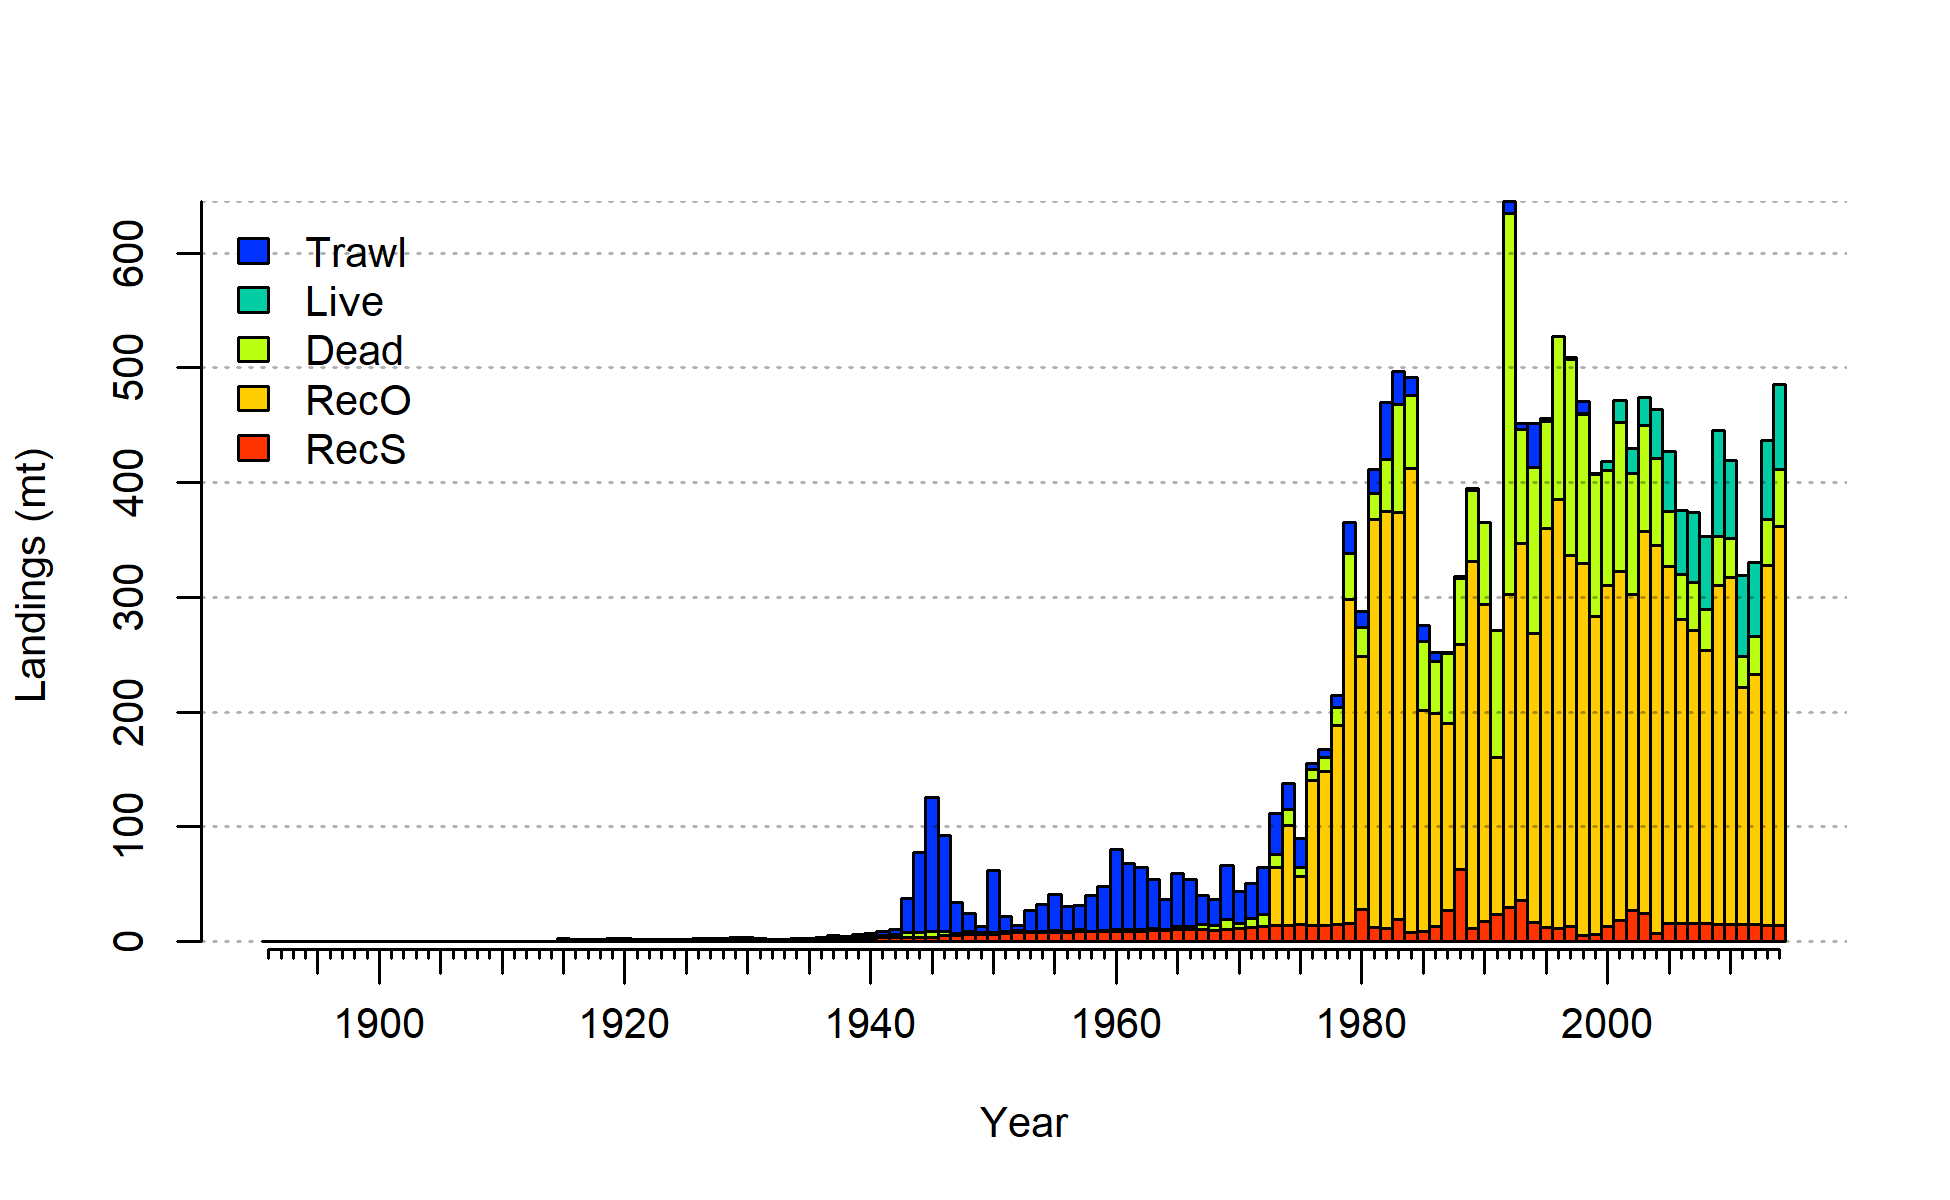
\includegraphics[width=1\textwidth,height=1\textheight]{C:/Users/Jason.Cope/Documents/Github/Sebastes_melanops_OR/Document/models/Reference model/plots/catch2 landings stacked.png}
\caption{Landings by fleet used in the reference model where catches in metric tons by fleet are stacked.\label{fig:es-catch}}
\end{figure}

\clearpage

\hypertarget{data-and-assessment}{%
\subsection*{Data and assessment}\label{data-and-assessment}}
\addcontentsline{toc}{subsection}{Data and assessment}

The first Black Rockfish stock assessment along the west coast of the United States that included the majority of Oregon waters was completed in 2007, covering the area south of Cape Falcon, Oregon to north of Point Piedros Blancos, California (\textbf{Sampson\_2007?}). In 2015, a subsequent assessment was completed that included Oregon waters only as one of three (also Washington and California) seperate assessment areas delineated by state lines (\textbf{Copeetal\_2015?}). Similarly, this assessment treats Oregon waters as a single assessment area. All of these assessments have used Stock Synthesis software. This assessment used Stock Synthesis version 3.30.21.00.

This assessment integrates data and information from multiple sources into one modeling framework. The stock assessment model for Black Rockfish is informed by catch data from two commercial fleets and two recreational fleets, six abundance indices, five sets of length composition data, and 3 sets of conditional age-at-length compositions. It also uses an ageing error matrix to incorporate ageing imprecision and applies fixed parameterizations of weight-at-length, maturity-at-length, and fecundity-at-length, the Beverton-Holt stock-recruitment steepness value and recruitment variability. Life history parameters were sex-specific (i.e., a two-sex model) with natural mortality fixed at external estimates and growth and recruitment parameters estimated. Additional parameters that were estimated include initial population scale (\(lnR_0\)), selectivity for each fishery and survey, and extra survey variance. The base model was tuned to account for the weighting of the length and age data and index variances (which was estimated), as well as the specification of the recruitment bias adjustments. Derived quantities include, among other things, the time series of spawning biomass, age and size structure, and current and projected future stock status. The model covers the years 1892 to 2022, with a 12 year forecast beginning in 2023.

Within model uncertainty is explicitly included in this assessment by parameter estimation uncertainty, while among model uncertainty is explored through sensitivity analyses addressing alternative input assumptions such as data treatment and weighting, and model specification sensitivity to the treatment of life history parameters, selectivity, recruitment, and survey catchability. A reference model was selected that best fit the observed data while concomitantly balancing the desire to capture the central tendency across those sources of uncertainty, ensure model realism and tractability, and promote robustness to potential model misspecification.

\hypertarget{stock-biomass-and-dynamics}{%
\subsection*{Stock biomass and dynamics}\label{stock-biomass-and-dynamics}}
\addcontentsline{toc}{subsection}{Stock biomass and dynamics}

Spawning output (in millions of eggs; meggs) instead of spawning biomass is used to report the functionally mature population scale because fecundity is nonlinearly related to body female weight. The estimated spawning output at the beginning of 2023 was 900 meggs (\textasciitilde95 percent asymptotic intervals: 855 to 944 meggs, Table \ref{tab:ssbES} and Figure \ref{fig:es-ssb}), which when compared to unfished spawning output (1,633) meggs gives a relative stock status level of 55 percent (\textasciitilde95 percent asymptotic intervals: 53 to 57 percent, Figure \ref{fig:es-depl}). Overall, spawning output declined with the onset of increasing commercial removals in the 1960s and continued to decline with the increase in recreational catches through the 1990s, even dropping below the target relative stock size from 1993 to 2008, before steadily increasing back above target since that time. The largest of the estimated recruitment pulses occurred in 2008 and was followed by several above average recruitment years in the early 2010s, which contributed to the increase in spawning output through the mid to late 2010s. The minimum relative stock size of 25 percent of unfished levels is estimated to have occurred in 1999. Accordingly, the stock has not been below the minimum stock size threshold (i.e., never overfished based on median estimates). Currently the stock is estimated above the management target of \(SO_{40\%}\) in 2023 and is estimated to have remained above the target since 2009 (Table \ref{tab:ssbES} and Figure \ref{fig:es-depl}).

\begingroup\fontsize{10}{12}\selectfont
\begingroup\fontsize{10}{12}\selectfont

\begin{longtable}[t]{r>{\centering\arraybackslash}p{1.57cm}>{\centering\arraybackslash}p{1.57cm}>{\centering\arraybackslash}p{1.57cm}>{\centering\arraybackslash}p{1.57cm}>{\centering\arraybackslash}p{1.57cm}>{\centering\arraybackslash}p{1.57cm}}
\caption{\label{tab:ssbES}Estimated recent trend in spawning output and the fraction unfished and the 95 percent intervals.}\\
\toprule
Year & Spawning Output & Lower Interval & Upper Interval & Fraction Unfished & Lower Interval & Upper Interval\\
\midrule
\endfirsthead
\caption[]{Estimated recent trend in spawning output and the fraction unfished and the 95 percent intervals. \textit{(continued)}}\\
\toprule
Year & Spawning Output & Lower Interval & Upper Interval & Fraction Unfished & Lower Interval & Upper Interval\\
\midrule
\endhead

\endfoot
\bottomrule
\endlastfoot
2005 & 810.95 & 788.57 & 833.33 & 0.59 & 0.58 & 0.60\\
2006 & 807.26 & 784.84 & 829.68 & 0.59 & 0.58 & 0.59\\
2007 & 808.45 & 785.98 & 830.91 & 0.59 & 0.58 & 0.59\\
2008 & 810.93 & 788.42 & 833.44 & 0.59 & 0.58 & 0.60\\
2009 & 816.26 & 793.70 & 838.81 & 0.59 & 0.59 & 0.60\\
2010 & 813.90 & 791.32 & 836.49 & 0.59 & 0.58 & 0.60\\
2011 & 814.31 & 791.69 & 836.94 & 0.59 & 0.58 & 0.60\\
2012 & 822.04 & 799.37 & 844.72 & 0.60 & 0.59 & 0.60\\
2013 & 829.99 & 807.28 & 852.70 & 0.60 & 0.60 & 0.61\\
2014 & 829.72 & 806.98 & 852.46 & 0.60 & 0.60 & 0.61\\
2015 & 823.86 & 801.10 & 846.63 & 0.60 & 0.59 & 0.61\\*
\end{longtable}
\endgroup{}
\endgroup{}


\begin{figure}
\centering
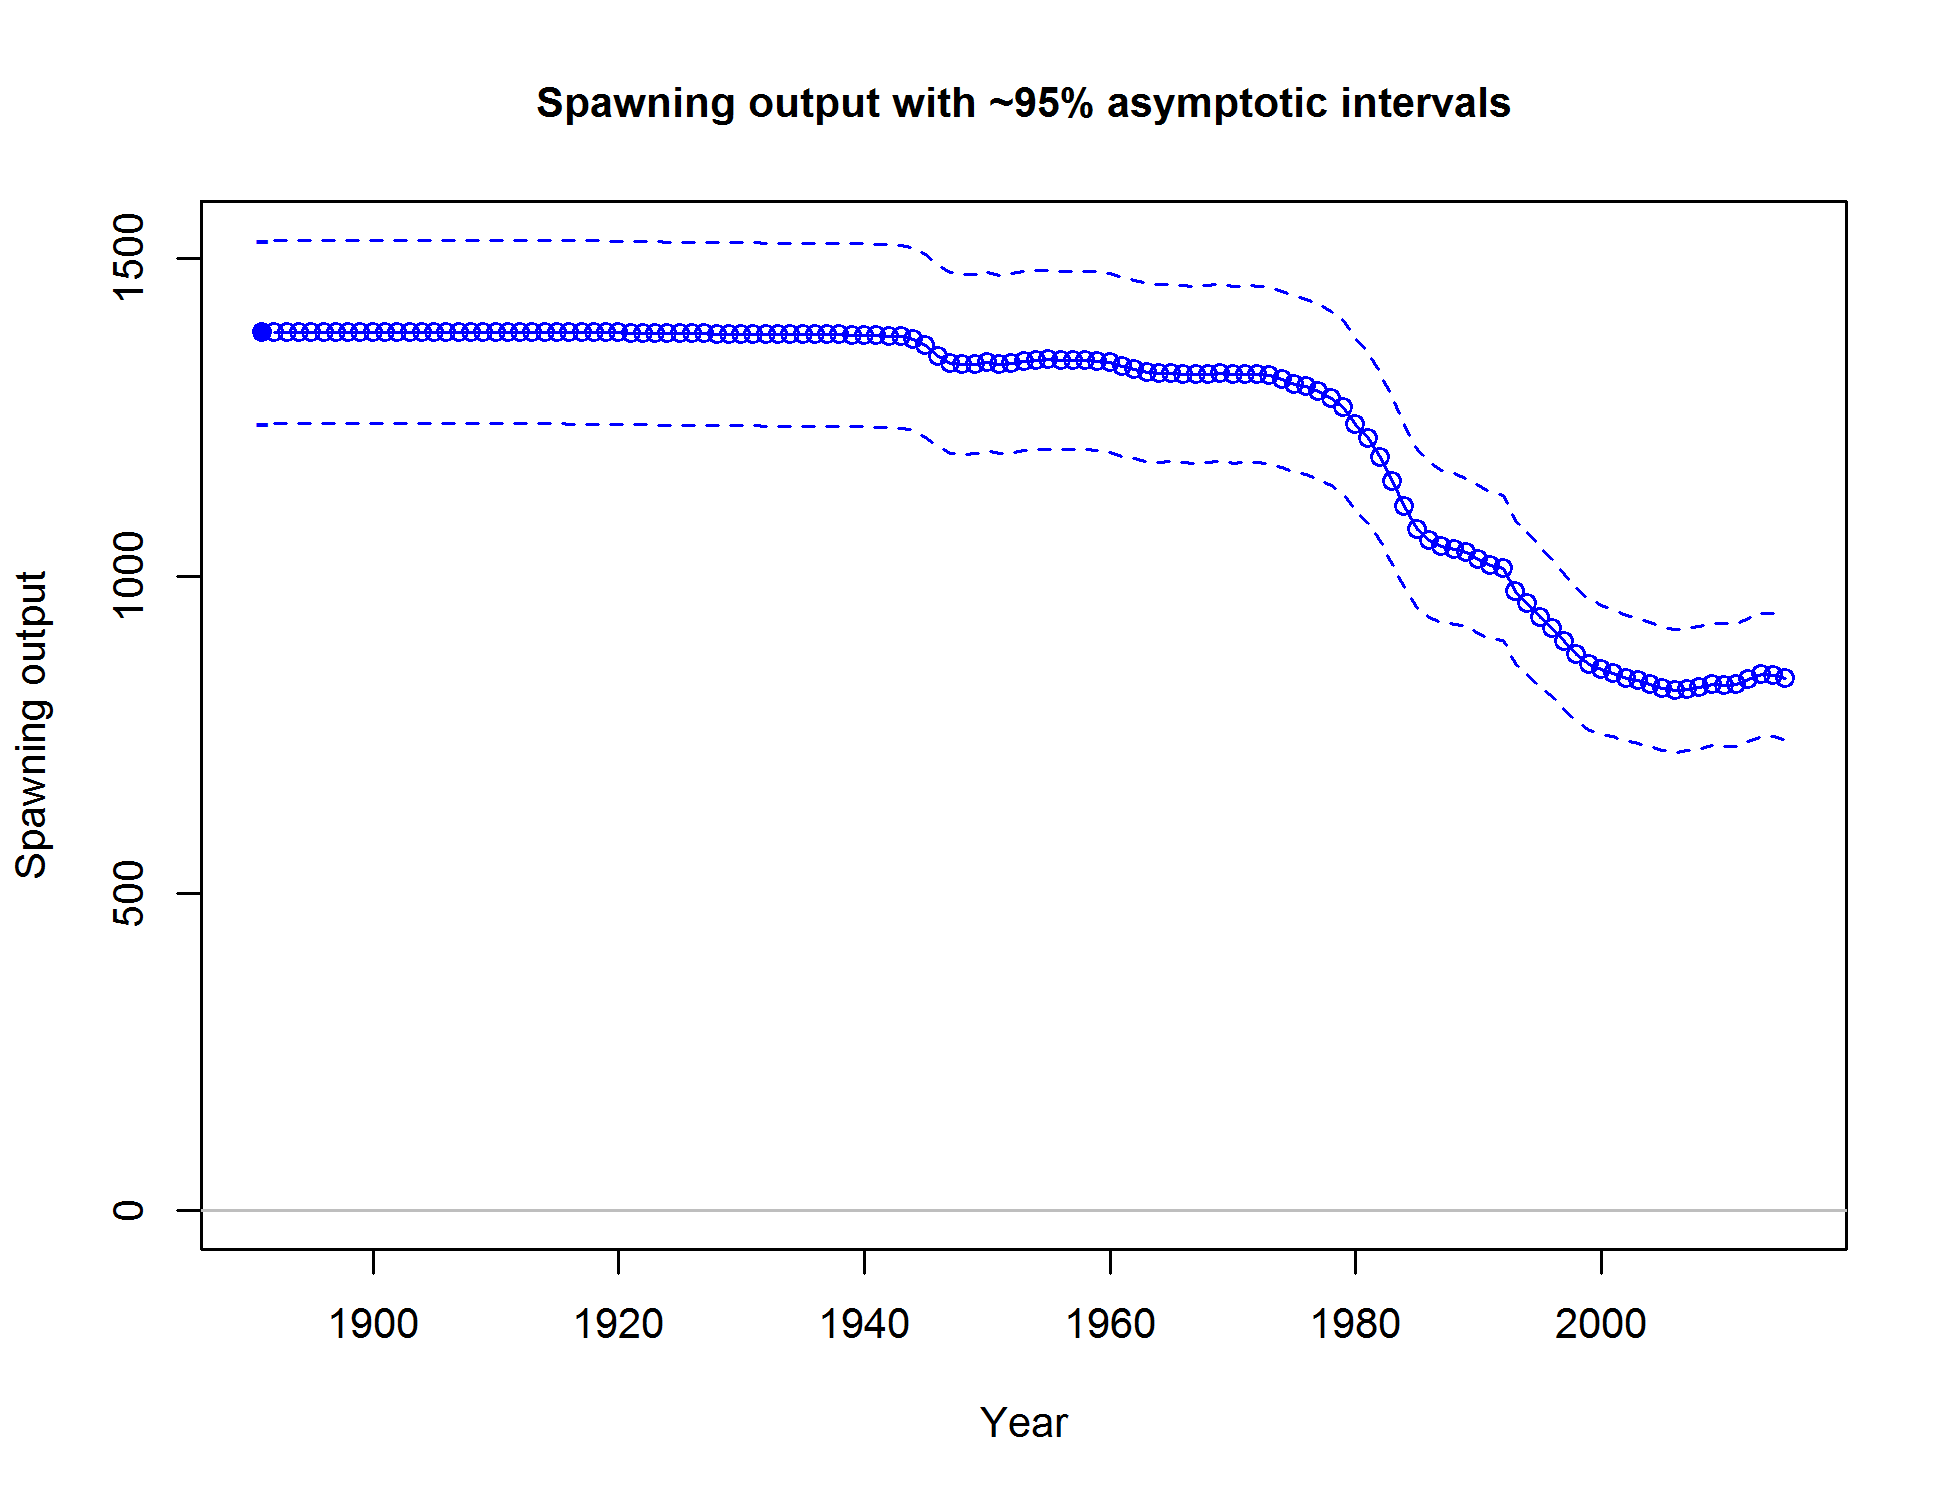
\includegraphics[width=1\textwidth,height=1\textheight]{C:/Users/Jason.Cope/Documents/Github/Sebastes_melanops_OR/Document/models/Reference model/plots/ts7_Spawning_output_with_95_asymptotic_intervals_intervals.png}
\caption{Estimated time series of spawning output (circles and line: median; light broken lines: 95 percent intervals) for the base model.\label{fig:es-ssb}}
\end{figure}

\begin{figure}
\centering
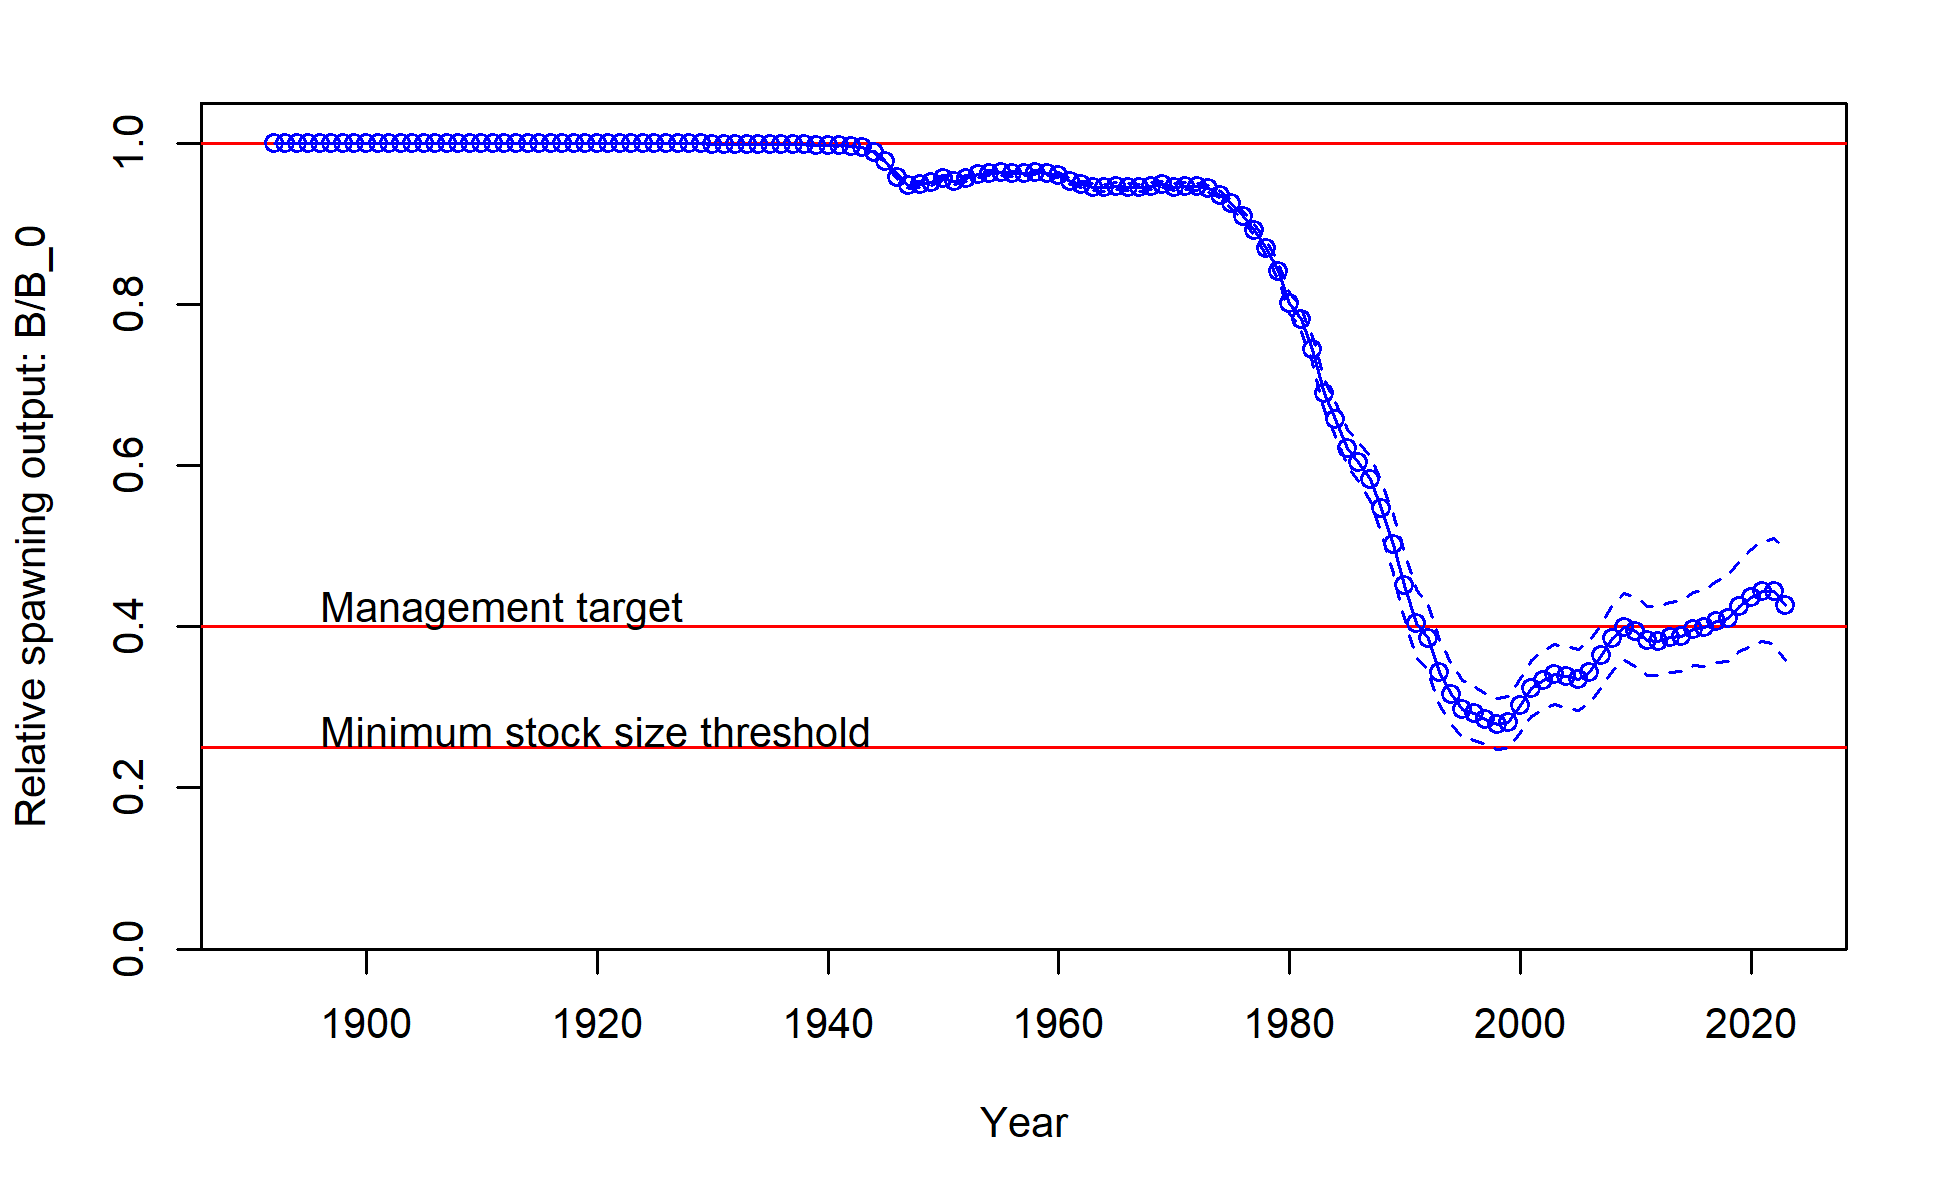
\includegraphics[width=1\textwidth,height=1\textheight]{C:/Users/Jason.Cope/Documents/Github/Sebastes_melanops_OR/Document/models/Reference model/plots/ts9_Relative_spawning_output_intervals.png}
\caption{Estimated time series of fraction of unfished spawning output (circles and line: median; light broken lines: 95 percent intervals) for the base model.\label{fig:es-depl}}
\end{figure}

\clearpage

\hypertarget{recruitment}{%
\subsection*{Recruitment}\label{recruitment}}
\addcontentsline{toc}{subsection}{Recruitment}

Recruitment is informed by the data from 1980 to 2017 (Table \ref{tab:recrES} and Figure \ref{fig:es-recruits}). The highest recruitment years occurred in 1999, 2000, 2008, 2013, and 2016. The large 2008 and 2016 year classes, as well as several above average year classes in the early 2010s, contributed to the recent increase in Black Rockfish biomass. Recruitment is informed by composition data and six relative abundance indices. The 2015 stock assessment did not estimate deviations from the stock-recruitment curve. While the Black Rockfish stock has been reduced to levels that theoretically would provide some information on how recruitment compensation changes across spawning biomass levels (i.e., inform the steepness parameter), the assessment model could not adequately estimate a reasonable steepness parameter. Thus, recruitment is based on a fixed assumption about steepness (\(h\) = 0.72) and recruitment variability (\(\sigma_R\) = 0.6).

\begingroup\fontsize{10}{12}\selectfont
\begingroup\fontsize{10}{12}\selectfont

\begin{longtable}[t]{r>{\centering\arraybackslash}p{2.2cm}>{\centering\arraybackslash}p{2.2cm}>{\centering\arraybackslash}p{2.2cm}>{\centering\arraybackslash}p{2.2cm}}
\caption{\label{tab:recrES}Estimated recent trend in recruitment (1,000s) and recruitment deviations and the 95 percent intervals for the model area.}\\
\toprule
Year & Recruitment (1,000s) & Interval & Recruitment Deviations & Interval\\
\midrule
\endfirsthead
\caption[]{Estimated recent trend in recruitment (1,000s) and recruitment deviations and the 95 percent intervals for the model area. \textit{(continued)}}\\
\toprule
Year & Recruitment (1,000s) & Interval & Recruitment Deviations & Interval\\
\midrule
\endhead

\endfoot
\bottomrule
\endlastfoot
2013 & 3,895 & 3,283–4,620 & 0.47 & 0.326–0.614\\
2014 & 3,481 & 2,880–4,207 & 0.36 & 0.196–0.522\\
2015 & 1,587 & 1,197–2,106 & -0.43 & -0.692–-0.167\\
2016 & 3,886 & 3,079–4,904 & 0.47 & 0.259–0.673\\
2017 & 1,009 & 623–1,637 & -0.93 & -1.401–-0.456\\
2018 & 2,906 & 2,695–3,133 & 0.00 & 0.000–0.000\\
2019 & 2,928 & 2,715–3,158 & 0.00 & 0.000–0.000\\
2020 & 2,946 & 2,730–3,179 & 0.00 & 0.000–0.000\\
2021 & 2,958 & 2,739–3,195 & 0.00 & 0.000–0.000\\
2022 & 2,962 & 2,737–3,204 & 0.00 & 0.000–0.000\\
2023 & 2,942 & 2,709–3,195 & 0.00 & 0.000–0.000\\*
\end{longtable}
\endgroup{}
\endgroup{}


\begin{figure}
\centering
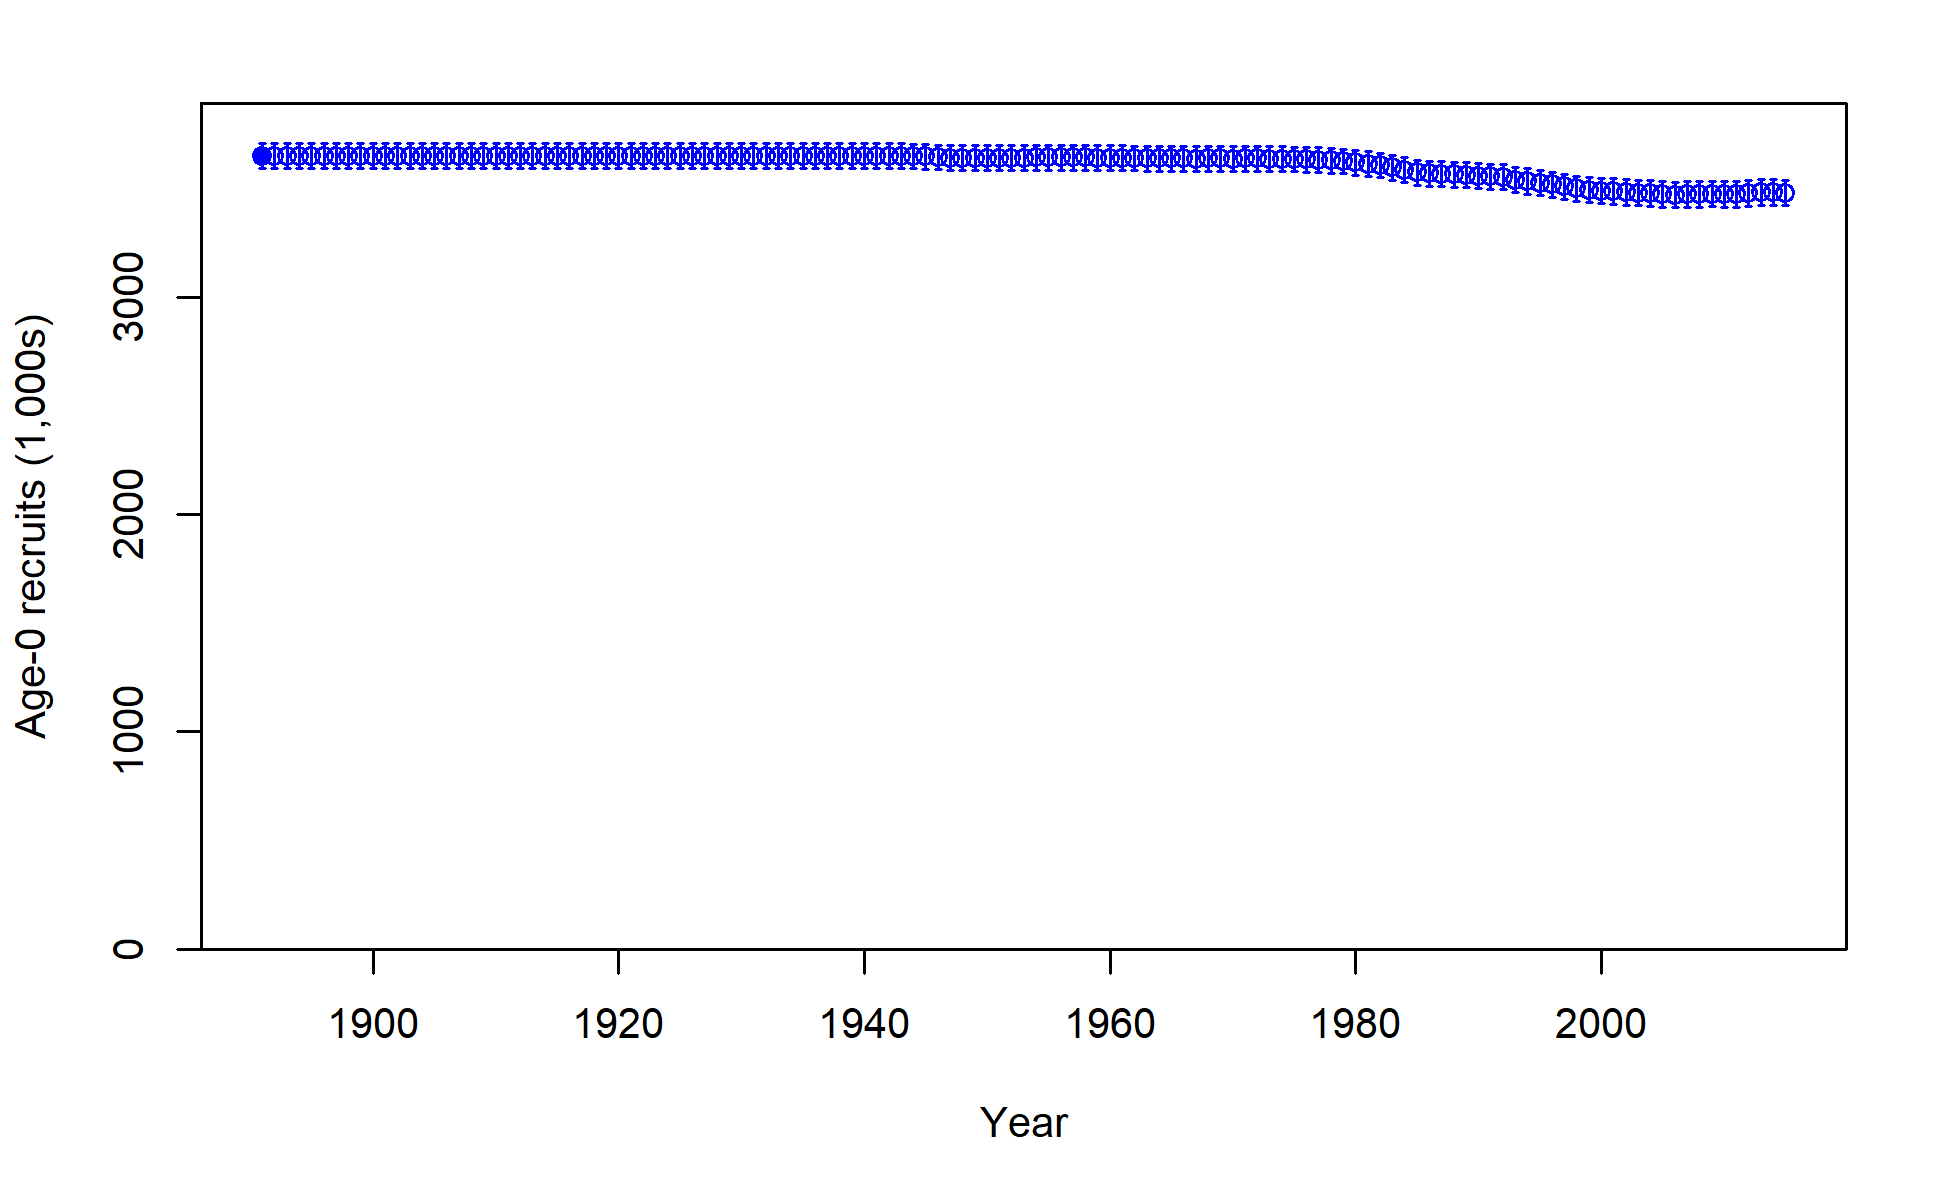
\includegraphics[width=1\textwidth,height=1\textheight]{C:/Users/Jason.Cope/Documents/Github/Sebastes_melanops_OR/Document/models/Reference model/plots/ts11_Age-0_recruits_(1000s)_with_95_asymptotic_intervals.png}
\caption{Estimated time series of age-0 recruits (1000s) for the base model with 95 percent intervals.\label{fig:es-recruits}}
\end{figure}

--- Three dashes at start/end comments this section out, hopefully\ldots{}

\hypertarget{estimated-time-series-of-recruitment-deviations.}{%
\subsection{\texorpdfstring{\protect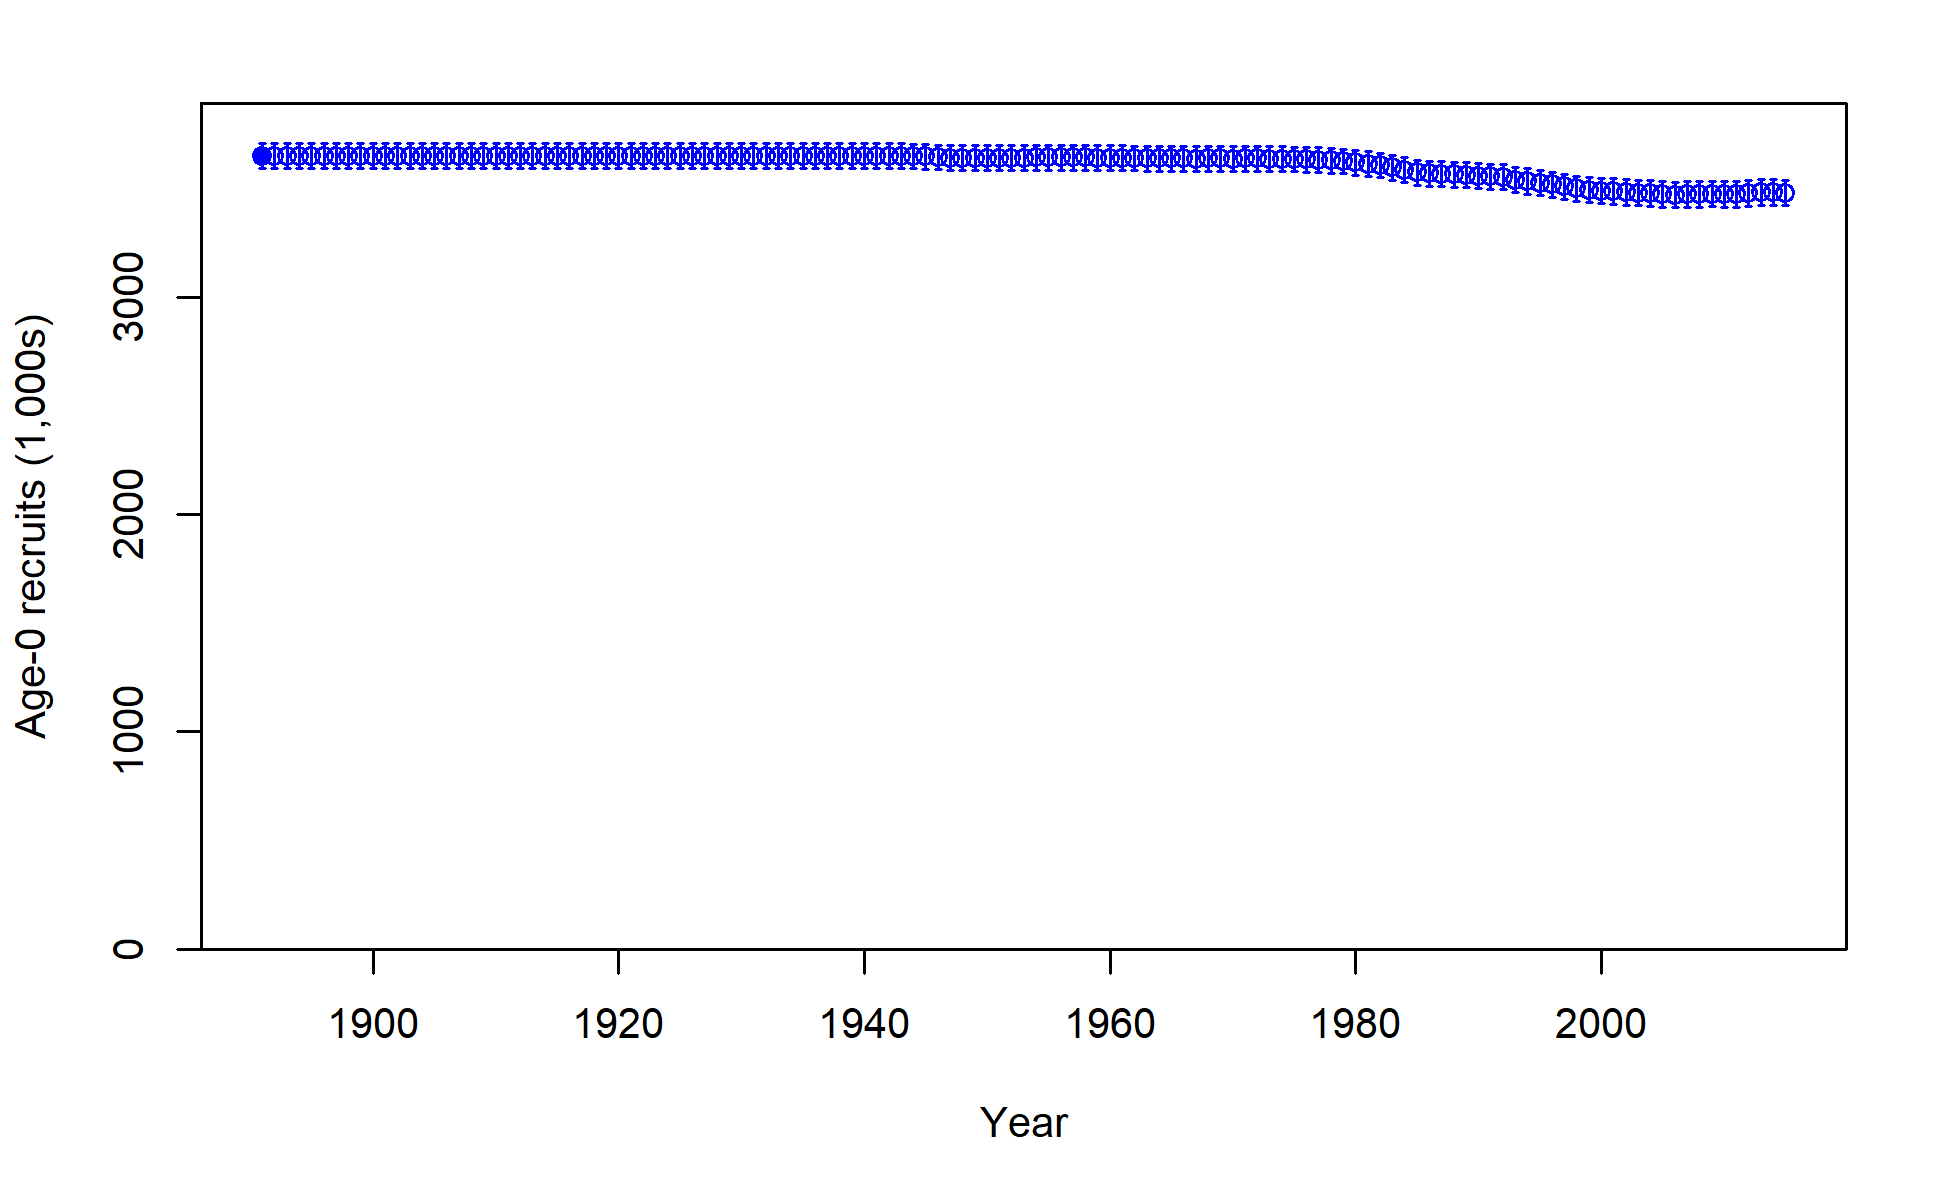
\includegraphics[width=1\textwidth,height=1\textheight]{C:/Users/Jason.Cope/Documents/Github/Sebastes_melanops_OR/Document/models/Reference model/plots/ts11_Age-0_recruits_(1000s)_with_95_asymptotic_intervals.png}}{Estimated time series of recruitment deviations.}}\label{estimated-time-series-of-recruitment-deviations.}}

\hypertarget{exploitation-status}\)) since 1980. Fishing was at or above the target rate from 1989 to 2005 and is slightly below it over the past 5 years (Table \ref{tab:exploitES} and Figures \ref{fig:es-1-spr} and \ref{fig:es-phase}), though the steepness value (0.72) indicates a lower value of SPR (or equivalently a higher fishing intensity than \(\text{SPR}_{50\%}\)) would be consistent with the biomass-based target of (\(\text{SO}_{40\%}\)) for sustainable removals. Trends in fishing intensity largely mirrored that of landings until the 1990s when recruitment pulses countered the catches somewhat to lower overall fishing intensity (Figure \ref{fig:es-1-spr}). The maximum fishing intensity was 0.7 in 1992, above the target SPR-based harvest rate of 0.50. The current level of 0.42 for 2022 is near the fishing limit. Fishing intensity over the past decade has ranged between 0.4 and 0.56 and the exploitation rate (0.04 - 0.08, Table \ref{tab:exploitES}) has come down since the time series high of 0.12 in 1992. Current estimates indicate that Black Rockfish spawning output is greater than than the target biomass level (\(\text{SO}_{40\%}\)), though fishing intensity remains near the target \(F_{MSY}\) proxy harvest rate of 1 - \(\text{SPR}_{50\%}\) (Figure \ref{fig:es-phase}).

\begingroup\fontsize{10}{12}\selectfont
\begingroup\fontsize{10}{12}\selectfont

\begin{longtable}[t]{r>{\centering\arraybackslash}p{1.57cm}>{\centering\arraybackslash}p{1.57cm}>{\centering\arraybackslash}p{1.57cm}>{\centering\arraybackslash}p{1.57cm}>{\centering\arraybackslash}p{1.57cm}>{\centering\arraybackslash}p{1.57cm}}
\caption{\label{tab:exploitES}Estimated recent trend in the 1-SPR where SPR is the spawning potential ratio the exploitation rate, and the  95 percent intervals.}\\
\toprule
Year & 1-SPR & Lower Interval & Upper Interval & Exploitation Rate & Lower Interval & Upper Interval\\
\midrule
\endfirsthead
\caption[]{Estimated recent trend in the 1-SPR where SPR is the spawning potential ratio the exploitation rate, and the  95 percent intervals. \textit{(continued)}}\\
\toprule
Year & 1-SPR & Lower Interval & Upper Interval & Exploitation Rate & Lower Interval & Upper Interval\\
\midrule
\endhead

\endfoot
\bottomrule
\endlastfoot
2005 & 0.39 & 0.39 & 0.40 & 0.05 & 0.05 & 0.05\\
2006 & 0.36 & 0.35 & 0.36 & 0.05 & 0.05 & 0.05\\
2007 & 0.35 & 0.35 & 0.36 & 0.05 & 0.05 & 0.05\\
2008 & 0.34 & 0.33 & 0.34 & 0.04 & 0.04 & 0.04\\
2009 & 0.40 & 0.40 & 0.41 & 0.05 & 0.05 & 0.06\\
2010 & 0.38 & 0.38 & 0.39 & 0.05 & 0.05 & 0.05\\
2011 & 0.31 & 0.31 & 0.32 & 0.04 & 0.04 & 0.04\\
2012 & 0.32 & 0.31 & 0.32 & 0.04 & 0.04 & 0.04\\
2013 & 0.39 & 0.38 & 0.40 & 0.05 & 0.05 & 0.05\\
2014 & 0.42 & 0.42 & 0.43 & 0.06 & 0.06 & 0.06\\*
\end{longtable}
\endgroup{}
\endgroup{}


\begin{figure}
\centering
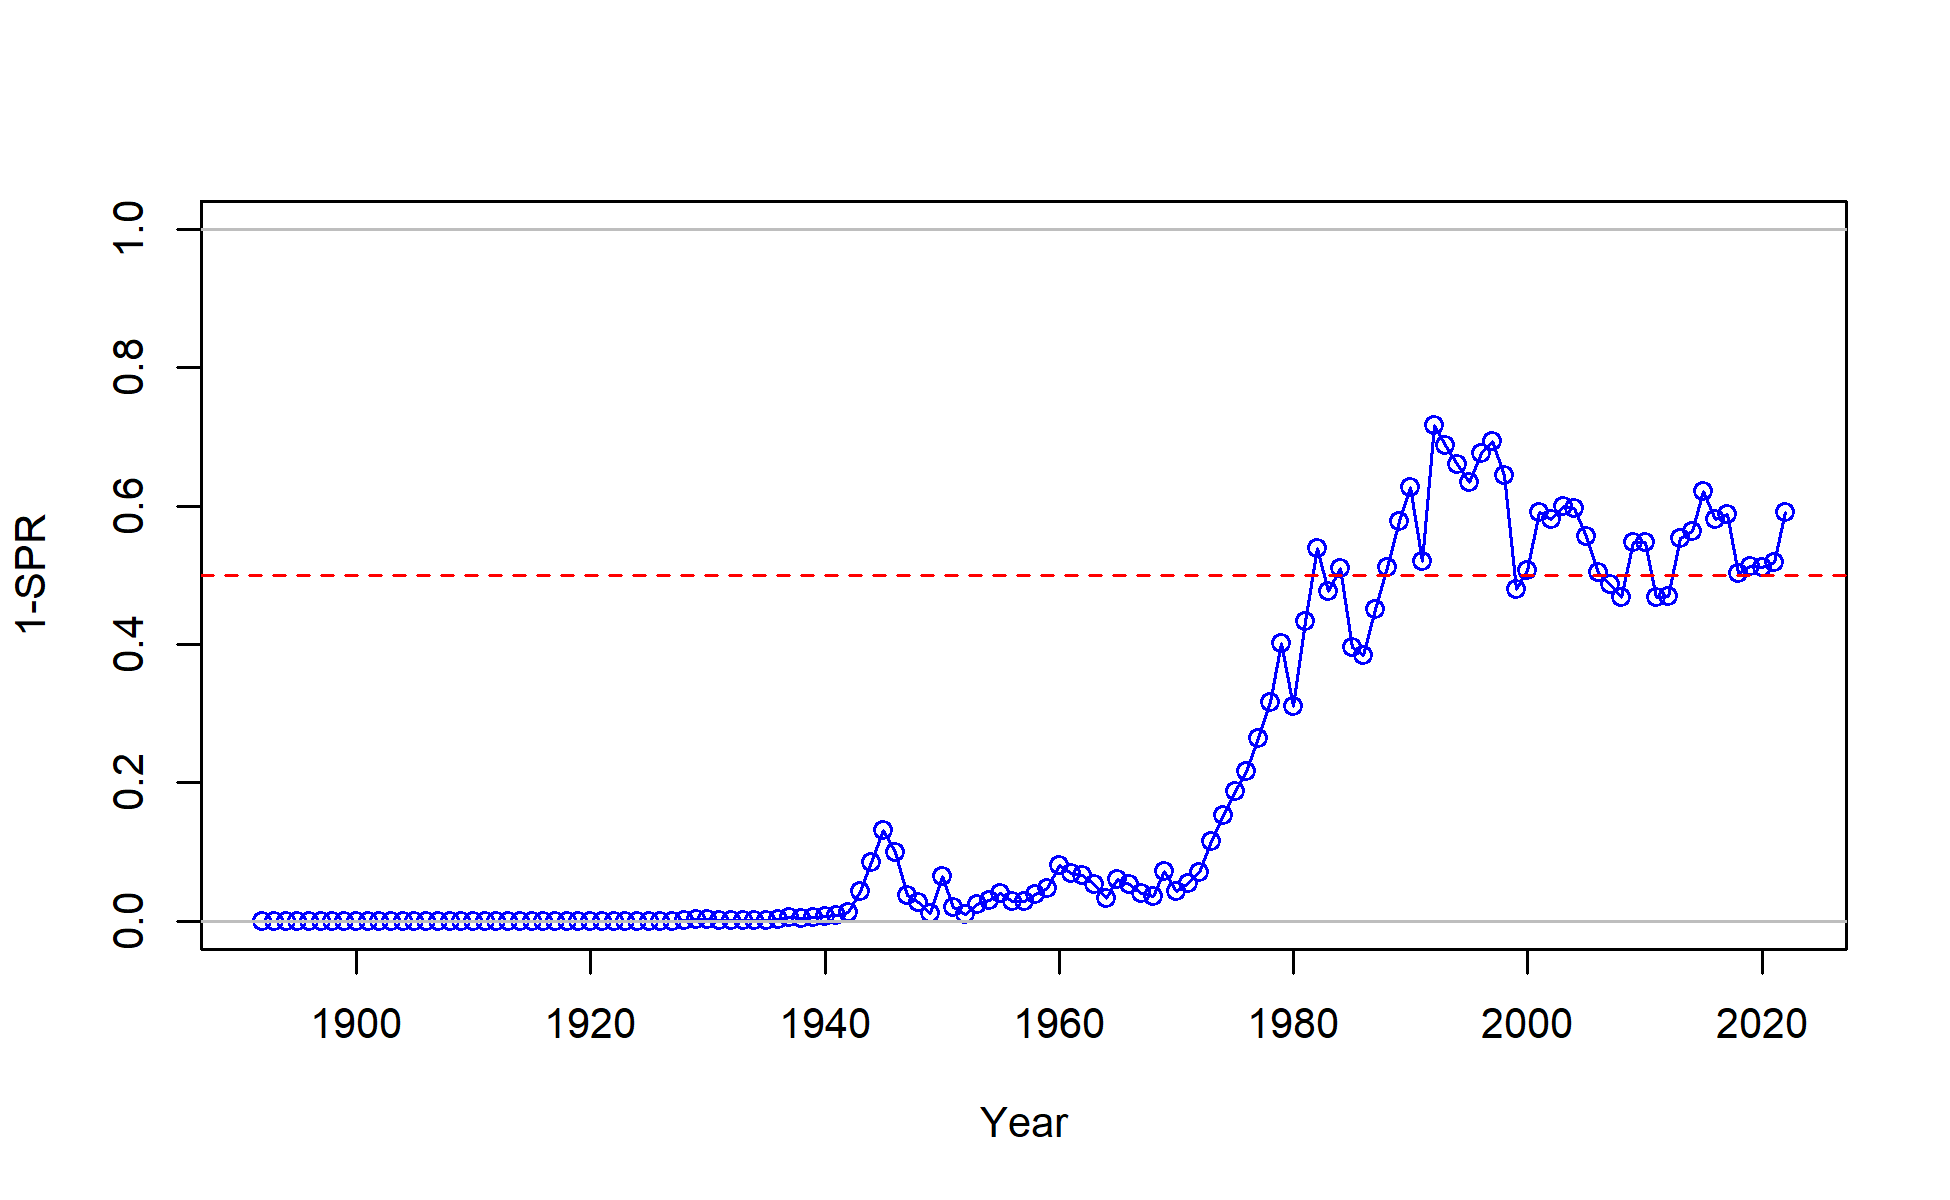
\includegraphics[width=1\textwidth,height=1\textheight]{C:/Users/Jason.Cope/Documents/Github/Sebastes_melanops_OR/Document/models/Reference model/plots/SPR2_minusSPRseries.png}
\caption{Estimated 1 - relative spawning ratio (SPR) by year for the base model. The management target is plotted as a red horizontal line and values above this reflect harvest in excess of the proxy harvest rate.\label{fig:es-1-spr}}
\end{figure}

\clearpage

\hypertarget{ecosystem-considerations}{%
\subsection*{Ecosystem considerations}\label{ecosystem-considerations}}
\addcontentsline{toc}{subsection}{Ecosystem considerations}

This stock assessment does not explicitly incorporate trophic interactions, habitat factors or environmental factors into the assessment model. More predation, diet and habitat work, and mechanistic linkages to environmental conditions would be needed to incorporate these elements into the stock assessment and should remain a priority. McClure et al. (2023) report the climate vulnerability for several west coast groundfishes, including Black Rockfish. Black Rockfish demonstrated both high biological sensitivity and high climate exposure risk, to give it an overall high vulnerability score to climate change. This result should also be considered with the fact that like many rockfishes, periods of low productivity is not unusually to Black Rockfish and their extended longevity has historically allowed them to wait for advantageous productivity periods. Additional stressors such as fishing and climate change that possibly truncate longevity could bring significant challenges to population sustainability.

\hypertarget{reference-points}\)), target relative biomass (40\%), and estimated selectivity and catch for each fleet (Table \ref{tab:referenceES}). The Black Rockfish population in Oregon at the start of 2023 is estimated to be 1.38 times (above) the target biomass, and fishing intensity during 2022 is estiamted to be 0.96 times (below) the fishing intensity target (Figure \ref{fig:es-phase}). The yield values are lower than the previous assessment for similar reference points due to updated life history estimates. The proxy MSY values of management quantities are the most conservative compared to the estimated MSY and MSY relative to 40\% biomass. Sustainable total yield, removals, using the proxy \(\text{SPR}_{50\%}\) is 455 mt. The spawning output equivalent to 40 percent of the unfished spawning output (\(\text{SO}_{40\%}\)) calculated using the SPR target (\(\text{SPR}_{50\%}\)) was 728.5 meggs. Recent removals have been close to the point estimate of potential long-term yields calculated using an \(\text{SPR}_{50\%}\) reference point, though the population size has continued to increase over recent years due to several above average recruitments. The equilibrium estimates of yield relative to biomass based on a steepness value fixed at 0.72 are provided in Figure \ref{fig:es-yield}, where vertical dashed lines indicate the estimate of fraction unfished at the start of 2023 (current) and the estimated management targets calculated based on the relative target biomass (B target), the SPR target, and the maximum sustainable yield (MSY).

The 2023 spawning biomass relative to unfished equilibrium spawning biomass, based on the 2022 fishing year, is above the management target of 40 percent of unfished spawning output (55\%). The relative biomass and the ratio of the estimated SPR to the management target (\(\text{SPR}_{50\%}\)) across all model years are shown in Figure \ref{fig:es-phase} where warmer colors (red) represent early years and colder colors (blue) represent recent years. There have been periods where the stock status has decreased below the target and fishing intensity has been higher than the target fishing intensity based on \(\text{SPR}_{50\%}\).

\begin{figure}
\centering
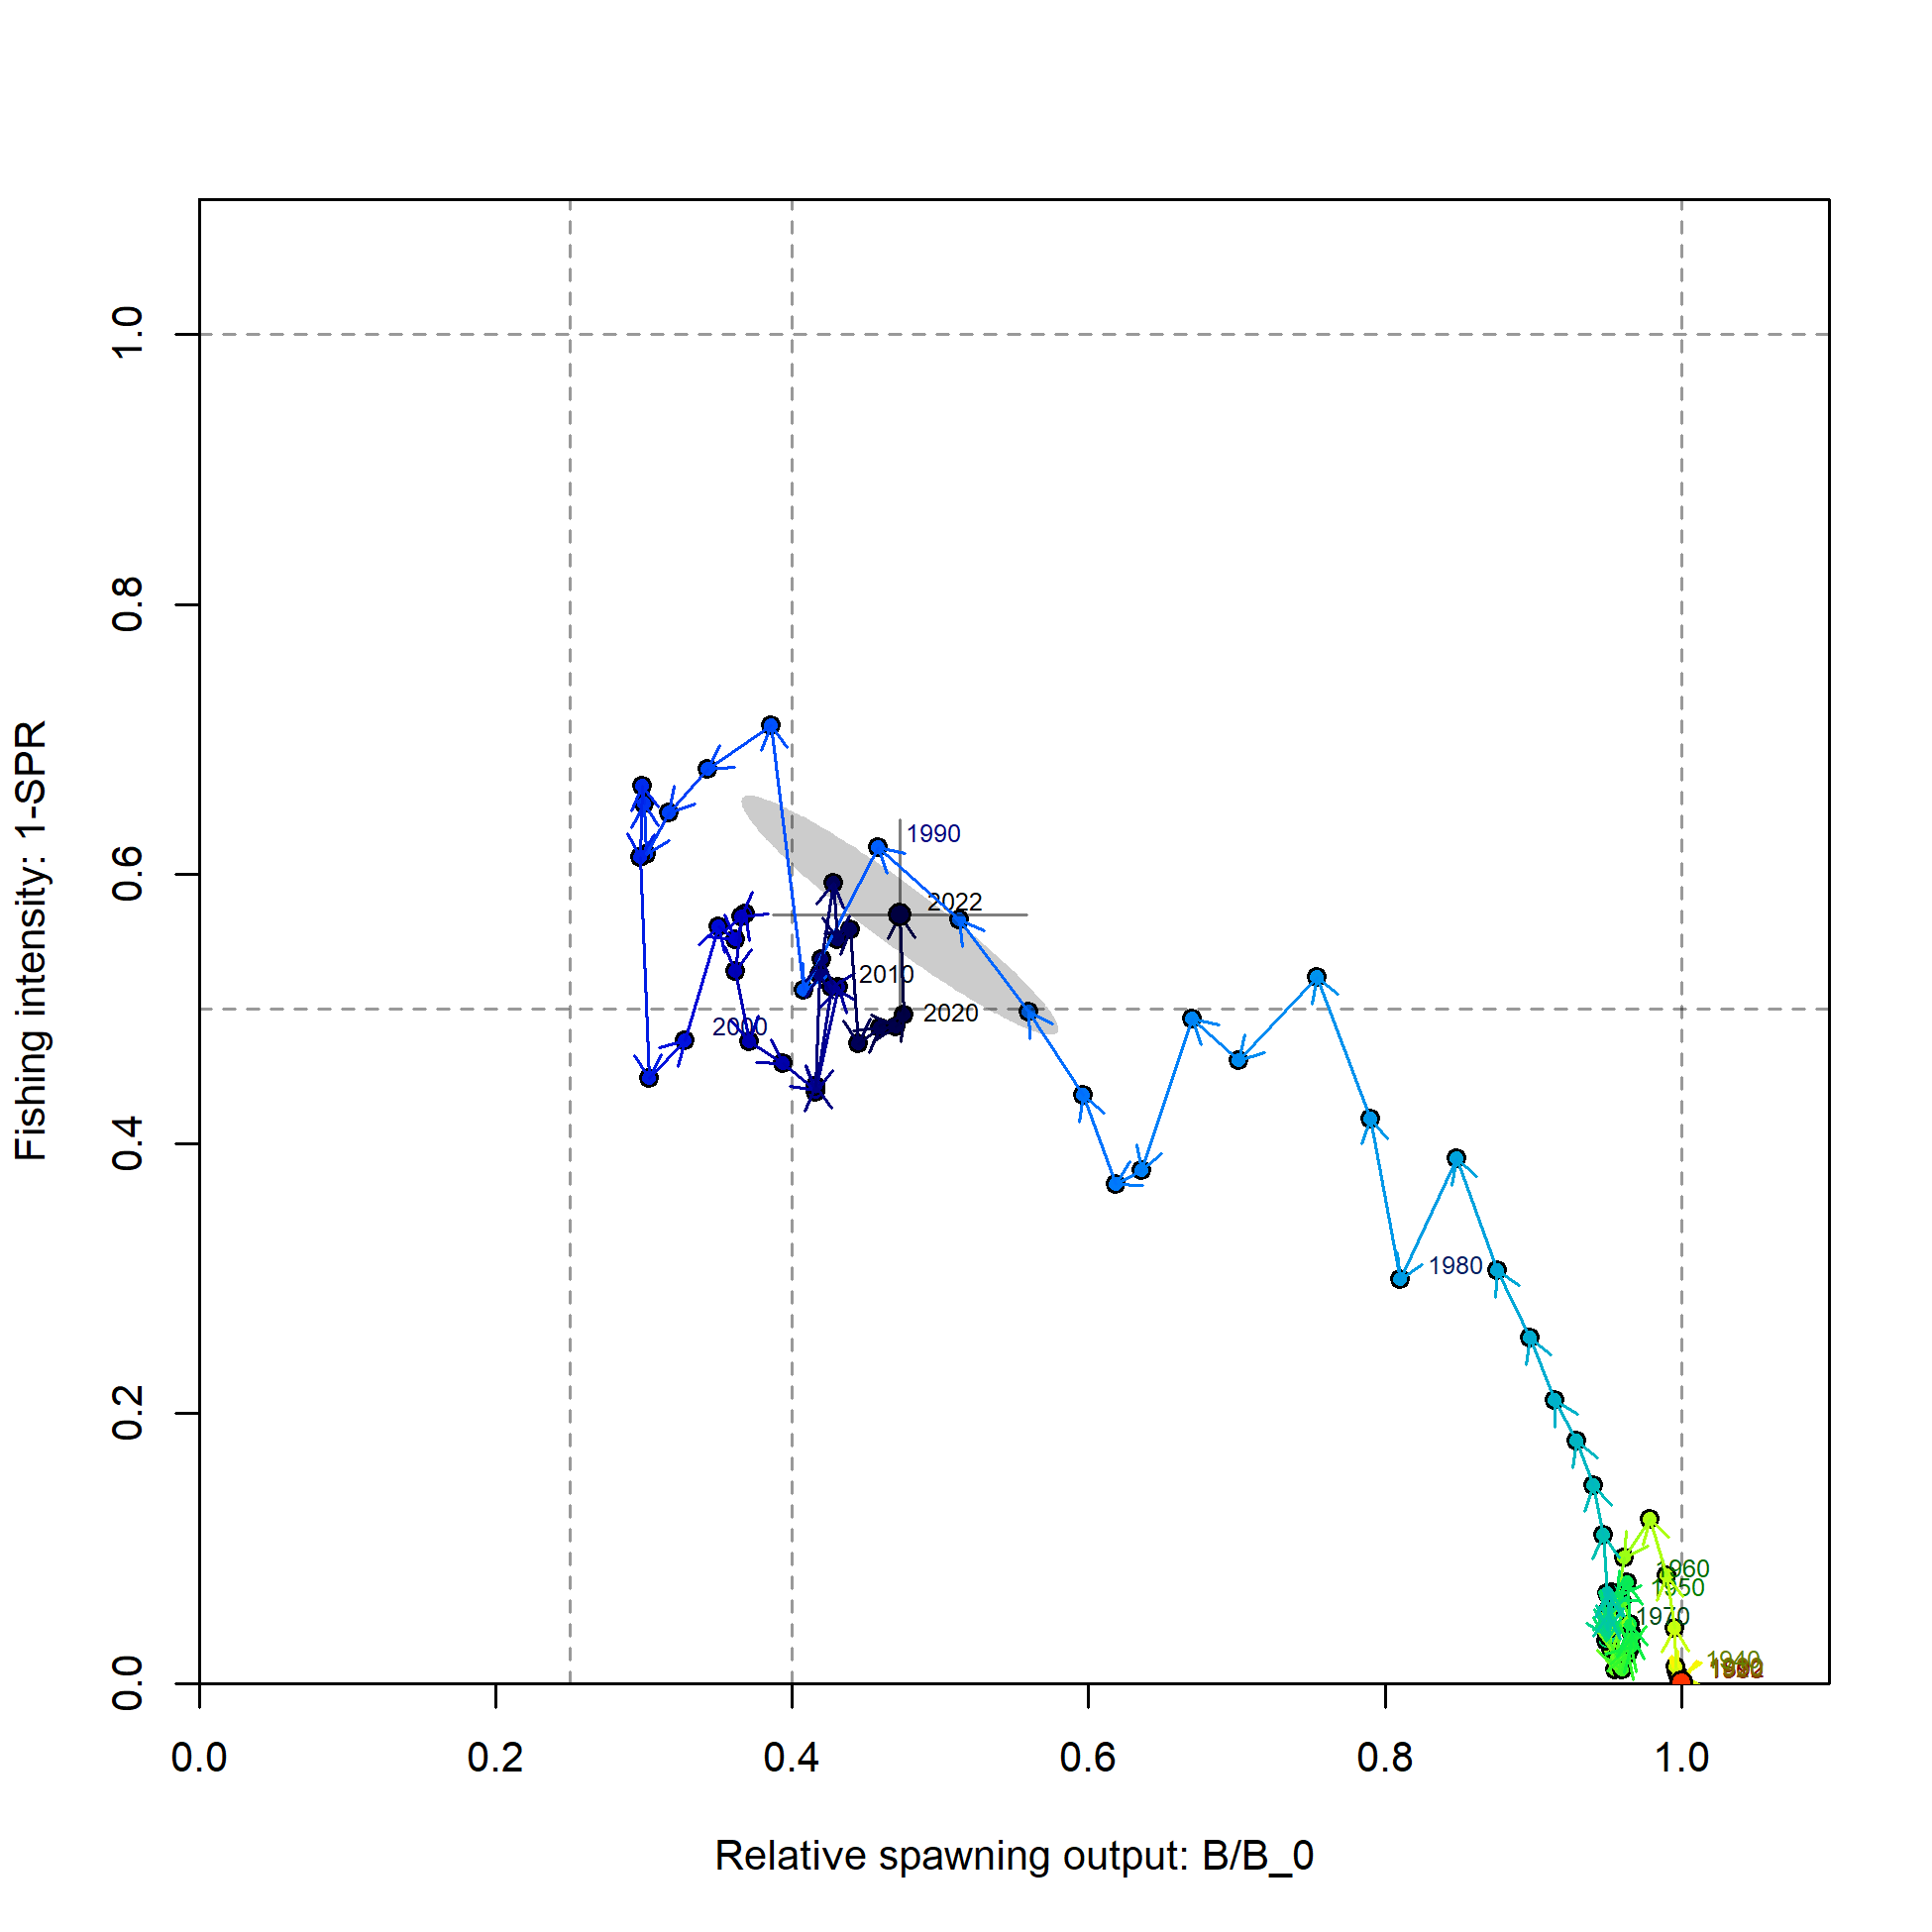
\includegraphics[width=1\textwidth,height=1\textheight]{C:/Users/Jason.Cope/Documents/Github/Sebastes_melanops_OR/Document/models/Reference model/plots/SPR4_phase.png}
\caption{Phase plot of estimated 1-SPR versus fraction unfished for the base model.\label{fig:es-phase}}
\end{figure}

\begin{figure}
\centering
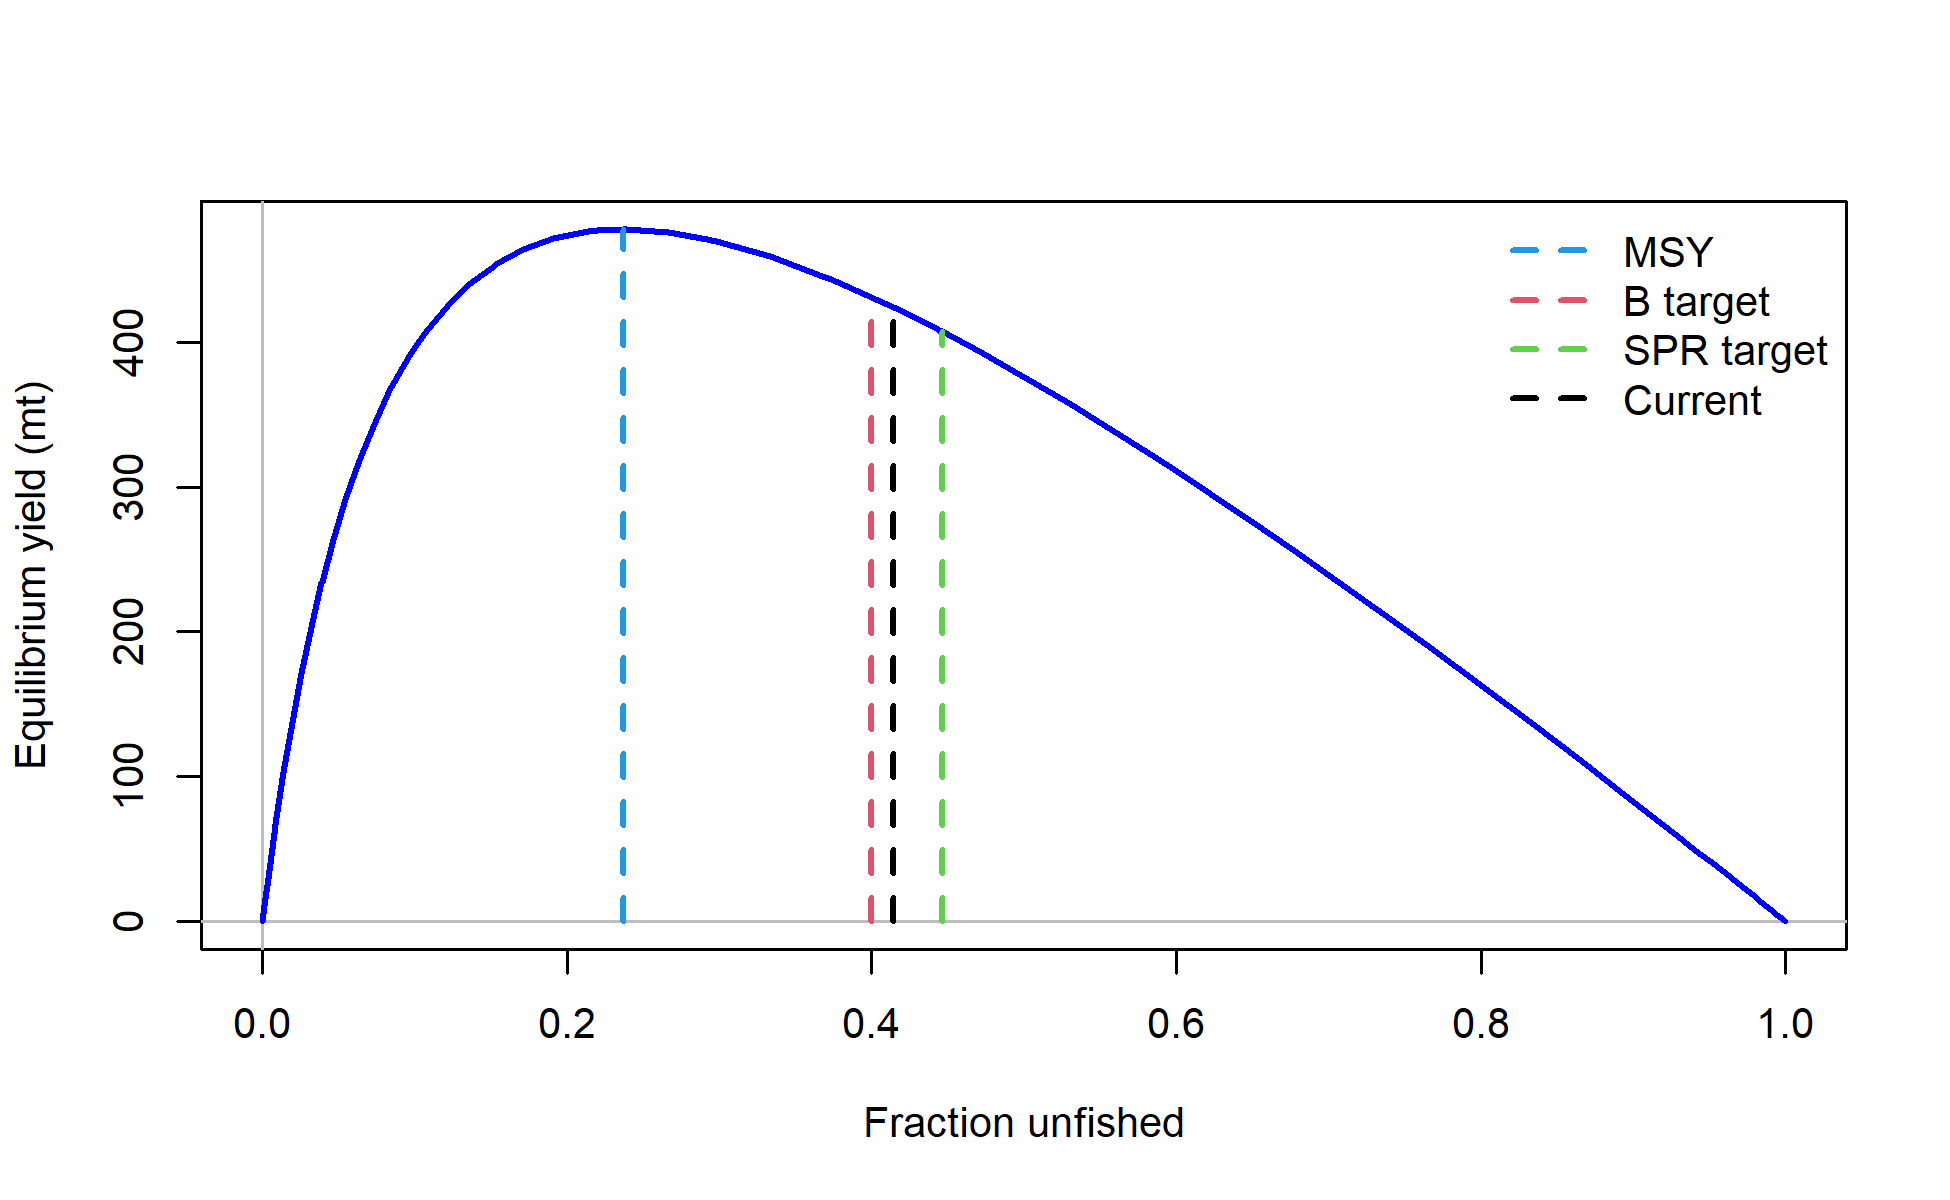
\includegraphics[width=1\textwidth,height=1\textheight]{C:/Users/Jason.Cope/Documents/Github/Sebastes_melanops_OR/Document/models/Reference model/plots/yield2_yield_curve_with_refpoints.png}
\caption{Equilibrium yield curve for the base case model. Values are based on (the time invariant) fishery selectivities and with steepness fixed at 0.72.\label{fig:es-yield}}
\end{figure}

\begingroup\fontsize{10}{12}\selectfont
\begingroup\fontsize{10}{12}\selectfont

\begin{longtable}[t]{r>{\centering\arraybackslash}p{2cm}>{\centering\arraybackslash}p{2cm}>{\centering\arraybackslash}p{2cm}}
\caption{\label{tab:referenceES}Summary of reference points and management quantities, including median estimates and associated 95 percent intervals.}\\
\toprule
 & Estimate & Lower Interval & Upper Interval\\
\midrule
\endfirsthead
\caption[]{Summary of reference points and management quantities, including median estimates and associated 95 percent intervals. \textit{(continued)}}\\
\toprule
 & Estimate & Lower Interval & Upper Interval\\
\midrule
\endhead

\endfoot
\bottomrule
\endlastfoot
Unfished Spawning Output & 1632.81 & 1577.19 & 1688.43\\
Unfished Age 0+ Biomass (mt) & 11576.10 & 11142.20 & 12010.00\\
Unfished Recruitment (R0) & 3807.86 & 3678.16 & 3937.56\\
Spawning Output (2023) & 899.77 & 855.05 & 944.49\\
Fraction Unfished (2023) & 0.55 & 0.53 & 0.57\\
Reference Points Based SB40\textbackslash{}\% & - & - & -\\
Proxy Spawning Output SB40\textbackslash{}\% & 653.12 & 630.88 & 675.37\\
SPR Resulting in SB40\textbackslash{}\% & 0.46 & 0.46 & 0.46\\
Exploitation Rate Resulting in SB40\textbackslash{}\% & 0.07 & 0.07 & 0.07\\
Yield with SPR Based On SB40\textbackslash{}\% (mt) & 481.51 & 464.00 & 499.03\\
Reference Points Based on SPR Proxy for MSY & - & - & -\\
Proxy Spawning Output (SPR50) & 728.48 & 703.67 & 753.30\\
SPR50 & 0.50 &   &  \\
Exploitation Rate Corresponding to SPR50 & 0.06 & 0.06 & 0.07\\
Yield with SPR50 at SB SPR (mt) & 454.96 & 438.30 & 471.63\\
Reference Points Based on Estimated MSY Values & - & - & -\\
Spawning Output at MSY (SB MSY) & 386.95 & 373.08 & 400.83\\
SPR MSY & 0.31 & 0.31 & 0.31\\
Exploitation Rate Corresponding to SPR MSY & 0.11 & 0.11 & 0.11\\
MSY (mt) & 533.65 & 514.71 & 552.60\\*
\end{longtable}
\endgroup{}
\endgroup{}


\clearpage

\hypertarget{management-performance}{%
\subsection*{Management performance}\label{management-performance}}
\addcontentsline{toc}{subsection}{Management performance}

Removals have been below the equivalent ABC-ACL since the prior assessment (Table ES-6), but those specified ABCs from the 2007 assessments are higher than those coming from the current assessment models. Removals over the last few years have or may have exceeded the newly estimated ABC-ACL values in some years. The differences in the treatment of natural mortality between the previous and current assessments are the biggest reason for this discrepancy.

Exploitation on Black Rockfish increased starting around 1960 and reached a high in the early 1990s. Since that time, catch has mostly fluctuated between 5 and 10 mt per year, with some years exceeding 10 mt, particularly in the last 4 years. The last ten years of the vermilion rockfish component acceptable biological catch (ABC) and annual catch limit (ACL) (which are equivalent) of the Minor Shelf Rockfish North Complex has been set, by definition, below the overfishing limit (OFL) (Table \ref{tab:ofl-es}). The Black Rockfish component OFL for this Complex has been exceeded by the Oregon removals in the most recent 4 years.

\#```\{r, results = `asis'\} \#yrs = hist = 2011:endyr \#nfleets = 2 \#catch = dead = est.dead = input.catch = 0 \#for (i in 1:nfleets)\{ \# name = paste0(``retain(B):\_``,i) \# input.catch = model\(timeseries[model\)timeseries\$Yr \%in\% yrs, name{]} \# catch = cbind(catch, input.catch)

\hypertarget{name-paste0deadb_i}{%
\section{name = paste0(``dead(B):\_``,i)}\label{name-paste0deadb_i}}

\hypertarget{est.dead-modeltimeseriesmodeltimeseriesyr-in-yrs-name}{%
\section{\texorpdfstring{est.dead = model\(timeseries[model\)timeseries\$Yr \%in\% yrs, name{]}}{est.dead = modeltimeseries{[}modeltimeseries\$Yr \%in\% yrs, name{]}}}\label{est.dead-modeltimeseriesmodeltimeseriesyr-in-yrs-name}}

\hypertarget{dead-cbinddead-est.dead}{%
\section{dead = cbind(dead, est.dead)}\label{dead-cbinddead-est.dead}}

\#\} \#total.catch \textless- round(apply(catch, 1, sum),1) \#total.dead \textless- round(apply(dead, 1, sum), 1)

\#man = read.csv(``C:/Users/Jason.Cope/Documents/Github/Vermilion rockfish OR WA assessment 2021/OR/write\_up/tables/\#vermilion\_man\_for\_doc.csv'') \#man = man{[}man\$Year \%in\% yrs, {]} \#out = cbind(man, total.catch, total.dead)

\#col\_names = c(``Year'', ``OFL'', ``ABC'', ``ACL'', ``Landings'', ``Est. Total Mortality'')

\#table\_format(x = out, \# caption = ``The OFL, ABC, ACL, landings, and the estimated total mortality in metric tons.'', \# label = ``ofl-es'', \# align = `l', \# col\_names = col\_names) \#```

\hypertarget{unresolved-problems-and-major-uncertainties}{%
\subsection*{Unresolved problems and major uncertainties}\label{unresolved-problems-and-major-uncertainties}}
\addcontentsline{toc}{subsection}{Unresolved problems and major uncertainties}

The most significant uncertainty for all models is the treatment and value of natural mortality and the form of fleet selectivity (e.g., length-based asymptotic vs.~age-based dome-shaped selectivity). Data-driven selection between the extreme ``kill'' (using a ramping of M) or ``hide'' hypotheses are not currently resolvable. The current California and Washington base models instead use a form of the ``kill'' hypothesis by not implementing the age-based selectivity (``hide'' hypothesis) and estimating female and male natural mortality, thus avoiding a fixing natural mortality as was necessary in the Oregon model. The Oregon model also contained a step in female natural mortality, a specification not used in the California or Washington models. Another important issue is the highly uncertain historical time-series of removals in all states, which needs further consideration. The development of fishery-dependent indices of abundance still requires further attention. Steepness, while fixed, is still highly uncertain for rockfishes and currently is mismatched to the MSY proxy. And while the steepness profile shows low sensitivity in several derived quantities, steepness strongly defines the yield capacity of stocks, and therefore could cause major uncertainty in the recommended management quantities. Stock structure and its relationship to the current political/management boundaries are also not fully understood, both within U.S. jurisdiction and between the U.S. and Canada. While this is a common challenge faced in most west coast stock assessments, further improvement on this topic will likely rely on black rockfish-specific data.

\hypertarget{scientific-uncertainty}{%
\subsection*{Scientific uncertainty}\label{scientific-uncertainty}}
\addcontentsline{toc}{subsection}{Scientific uncertainty}

The model-estimated uncertainty around the 2023 spawning biomass was \(\sigma\) = 0.03 and the uncertainty around the OFL was \(\sigma\) = 0.01. This is likely an underestimate of overall uncertainty because of the necessity to fix some parameters such as steepness, as well as a lack of explicit incorporation of model structural uncertainty.

\hypertarget{harvest-projections-and-decision-table}{%
\subsection*{Harvest Projections and Decision Table}\label{harvest-projections-and-decision-table}}
\addcontentsline{toc}{subsection}{Harvest Projections and Decision Table}

Black rockfish assessments for California and Washington have a preliminary distinction as category 1 stock assessments, thus harvest projections and decision tables are based on using P\emph{=0.45 and sigma = 0.36, resulting in a multiplier on the OFL of 0.956. The Oregon black rockfish assessment is a category 2 assessment, with a P}=0.45 and sigma = 0.72 with a multiplier of 0.913 applied to the OFL. These multipliers are also combined with the rockfish MSY proxy of FSPR=50\% MSY and the 40-10 harvest control rule to calculate OFLs, ABCs and ACLs. Projections for each state are provided in Table ES-7 to Table ES-9.

Uncertainty in management quantities for the base model of each state was characterized by exploring various model specifications in a decision table. Initial exploration included natural mortality and steepness values, and uncertainty in historical trawl catches for the WA and CA models. OR explored the scale factor coming from the value of the tagging catchability (Q) parameter, as well as M values. For the CA and WA models, there was very little sensitivity to steepness and trawl catches, but natural mortality produced sensitive results of predicted population scale and status. Discussion with the STAR panel resulted in high and low states of nature +/- 0.03 from the base case natural mortality values for females and males. High and low catch streams (rows) were determined by the forecasts, as described above, for each state of nature. Thus the low catch stream is based on the forecast from the low state of nature. The OR model demonstrated little sensitivity to M, but high sensitivity to the tagging survey Q. High and low states of nature, respectively, were based on a fixed tag of Q = 0.125 and Q estimated by the model. Resultant decision tables are provided in Table ES-10 to Table ES-12.

A ten year (2023-2032) projection of the reference model with removals in 2021 and 2022 provided by the Groundfish Management Team for each fleet under the category 1 (sigma=0.5) time-varying buffer using \(P^*\) = 0.45 and 40-10 ABC control rule is provided in Table \ref{tab:project_ES}.

\begingroup\fontsize{9}{11}\selectfont
\begingroup\fontsize{9}{11}\selectfont

\begin{longtable}[t]{c>{\centering\arraybackslash}p{1.38cm}>{\centering\arraybackslash}p{1.38cm}>{\centering\arraybackslash}p{1.38cm}>{\centering\arraybackslash}p{1.38cm}>{\centering\arraybackslash}p{1.38cm}>{\centering\arraybackslash}p{1.38cm}>{\centering\arraybackslash}p{1.38cm}}
\caption{\label{tab:project-ES}Projections of potential OFLs (mt), ABCs (mt), the buffer (ABC = buffer x OFL), estimated total biomass, spawning output, and fraction unfished.}\\
\toprule
Year & Predicted OFL & ABC Catch & Buffer & Summary Biomass & Spawning Output & Fraction Unfished\\
\midrule
\endfirsthead
\caption[]{Projections of potential OFLs (mt), ABCs (mt), the buffer (ABC = buffer x OFL), estimated total biomass, spawning output, and fraction unfished. \textit{(continued)}}\\
\toprule
Year &  Predicted OFL & ABC Catch & Buffer & Summary Biomass & Spawning Output & Fraction Unfished\\
\midrule
\endhead

\endfoot
\bottomrule
\endlastfoot
2023	&	541.9	&	496.5	&	1.00	&	7981.8	 &	899.8	&	0.55\\
2024	&	-	&	-	&	-	&	-	 &	-	&	-\\
2025	&	-	&	-	&	-	&	-	 &	-	&	-\\
2026	&	-	&	-	&	-	&	-	 &	-	&	-\\
2027	&	-	&	-	&	-	&	-	 &	-	&	-\\
2028	&	-	&	-	&	-	&	-	 &	-	&	-\\
2029	&	-	&	-	&	-	&	-	 &	-	&	-\\
2030	&	-	&	-	&	-	&	-	 &	-	&	-\\
2031	&	-	&	-	&	-	&	-	 &	-	&	-\\
2032	&	-	&	-	&	-	&	-	 &	-	&	-\\
2033	&	-	&	-	&	-	&	-	 &	-	&	-\\
2034	&	-	&	-	&	-	&	-	 &	-	&	-\\*
\end{longtable}
\endgroup{}
\endgroup{}


The decision table (Table \ref{tab:es-dec-tab}) was constructed using female and male natural mortality to define the low and high states of nature. The multi-parameter likelihood profile was used to find the low (Female M = 0.07092; Male M= 0.06525) and high (Female M = 0.08527; Male M = 0.07845) female and male natural mortality values that produce -log likeliehood values +0.66 units from the reference -log likelihood value. These correspond to the 12.5\% and 87.5\% quantiles (standard quantiles used in west coast decision tables). The catch rows in the table were based on three proposed catch streams: 1. P* = 0.45, sigma = 0.5 2. P* = 0.40, sigma = 0.5 3. An equilibrium catch based on the \(F_{MSY}\) proxy using SPR = 0.5.

Across all states of natures and catch streams, vermilion rockfish relative stock size never falls below the target relative stock size of 40\%. Both P* approaches lower the stock status from the high relative stock size values, while the \(F_{MSY}\) proxy does not. The mismatch in the corresponding steepness value (\(h=0.6\)) that matches MSY at SPR = 0.5 with the steepness value in the stock assessment (\(h=0.72\)) that correpsonds to an MSY SPR of 0.35 explains why this constant catch will maintain the stock at very high relative stock status levels.

\clearpage

\begingroup\fontsize{9}{11}\selectfont
\begingroup\fontsize{9}{11}\selectfont

\begin{longtable}[t]{l>{\raggedright\arraybackslash}p{0.08\linewidth}>{\raggedright\arraybackslash}p{0.08\linewidth}>{\raggedright\arraybackslash}p{0.1\linewidth}>{\raggedright\arraybackslash}p{0.09\linewidth}>{\raggedright\arraybackslash}p{0.1\linewidth}>{\raggedright\arraybackslash}p{0.09\linewidth}>{\raggedright\arraybackslash}p{0.1\linewidth}>{\raggedright\arraybackslash}p{0.09\linewidth}}
\caption{\label{tab:es-dec-tab}Decision table summary of 10 year projections beginning in 2023 for alternative states of nature based on an axis of uncertainty related to model structure relative to the reference model (i.e., estimate catchability, Q, associated with the acoustic-visual survey and no estimation of recruitment deviations) . Columns range over low (12.5 quantile), mid (reference model), and high states (87.5 quantile) of nature and rows range over different catch level assumptions. Values in italics indicate years where the stock size prevented the full catch removals.}\\
\toprule
\multicolumn{3}{c}{ } & \multicolumn{2}c{Estimate Q} & \multicolumn{2}c{Reference Model} & \multicolumn{2}c{No Rec Devs} \\
\cmidrule(l{3pt}r{3pt}){4-5} \cmidrule(l{3pt}r{3pt}){6-7} \cmidrule(l{3pt}r{3pt}){8-9}
  & Year & Catch & Spawning Output & Fraction Unfished & Spawning Output & Fraction Unfished & Spawning Output & Fraction Unfished\\
\hline
	&	2023	&	-	&	 - 	&	-	&	 - 	&	-	&	 - 	&	-\\	
	&	2024	&	-	&	 - 	&	-	&	 - 	&	-	&	 - 	&	-\\	
	&	2025	&	-	&	 - 	&	-	&	 - 	&	-	&	 - 	&	-\\
	&	2026	&	-	&	 - 	&	-	&	 - 	&	-	&	 - 	&	-\\
	&	2027	&	-	&	 - 	&	-	&	 - 	&	-	&	 - 	&	-\\
P*=0.45	&	2028	&	-	&	 - 	&	-	&	 - 	&	-	&	 - 	&	-\\
sigma=0.5	&	2029	&	-	&	 - 	&	-	&	 - 	&	-	&	 - 	&	-\\
	&	2030	&	-	&	 - 	&	-	&	 - 	&	-	&	 - 	&	-\\
	&	2031	&	-	&	 - 	&	-	&	 - 	&	-	&	 - 	&	-\\
	&	2032	&	-	&	 - 	&	-	&	 - 	&	-	&	 - 	&	-\\
	&	2033	&	-	&	 - 	&	-	&	 - 	&	-	&	 - 	&	-\\
	&	2034	&	-	&	 - 	&	-	&	 - 	&	-	&	 - 	&	-\\
\hline																
	&	2023	&	-	&	 - 	&	-	&	 - 	&	-	&	 - 	&	-\\
	&	2024	&	-	&	 - 	&	-	&	 - 	&	-	&	 - 	&	-\\
	&	2025	&	-	&	 - 	&	-	&	 - 	&	-	&	 - 	&	-\\
	&	2026	&	-	&	 - 	&	-	&	 - 	&	-	&	 - 	&	-\\
	&	2027	&	-	&	 - 	&	-	&	 - 	&	-	&	 - 	&	-\\
P*=0.4	&	2028	&	-	&	 - 	&	-	&	 - 	&	-	&	 - 	&	-\\
sigma=0.5	&	2029	&	-	&	 - 	&	-	&	 - 	&	-	&	 - 	&	-\\
	&	2030	&	-	&	 - 	&	-	&	 - 	&	-	&	 - 	&	-\\
	&	2031	&	-	&	 - 	&	-	&	 - 	&	-	&	 - 	&	-\\
	&	2032	&	-	&	 - 	&	-	&	 - 	&	-	&	 - 	&	-\\
	&	2033	&	-	&	 - 	&	-	&	 - 	&	-	&	 - 	&	-\\
	&	2034	&	-	&	 - 	&	-	&	 - 	&	-	&	 - 	&	-\\
\hline																
	&	2023	&	-	&	 - 	&	-	&	 - 	&	-	&	 - 	&	-\\
	&	2024	&	-	&	 - 	&	-	&	 - 	&	-	&	 - 	&	-\\
	&	2025	&	-	&	 - 	&	-	&	 - 	&	-	&	 - 	&	-\\
	&	2026	&	-	&	 - 	&	-	&	 - 	&	-	&	 - 	&	-\\
Equilibrium	&	2027	&	-	&	 - 	&	-	&	 - 	&	-	&	 - 	&	-\\
yield from	&	2028	&	-	&	 - 	&	-	&	 - 	&	-	&	 - 	&	-\\
FMSY proxy	&	2029	&	-	&	 - 	&	-	&	 - 	&	-	&	 - 	&	-\\
of SPR=0.5	&	2030	&	-	&	 - 	&	-	&	 - 	&	-	&	 - 	&	-\\
	&	2031	&	-	&	 - 	&	-	&	 - 	&	-	&	 - 	&	-\\
	&	2032	&	-	&	 - 	&	-	&	 - 	&	-	&	 - 	&	-\\
	&	2033	&	-	&	 - 	&	-	&	 - 	&	-	&	 - 	&	-\\
	&	2034	&	-	&	 - 	&	-	&	 - 	&	-	&	 - 	&	-\\*
\hline
\end{longtable}
\endgroup{}
\endgroup{}


\clearpage

\hypertarget{research-and-data-needs}{%
\subsection*{Research and data needs}\label{research-and-data-needs}}
\addcontentsline{toc}{subsection}{Research and data needs}

Recommended avenues for research to help improve future black rockfish stock assessments:

\begin{enumerate}
\def\labelenumi{\arabic{enumi}.}
\tightlist
\item
  Further investigation into the movement and behavior of older (\textgreater{} age 10) females to reconcile their absence in fisheries data. If the females are currently inaccessible to fishing gear, can we find where they are?
\item
  Appropriate natural mortality values for females and males. This will help resolve the extent to which dome-shaped age-based selectivity may be occurring for each.
\item
  All states need improved historical catch reconstructions. The trawl fishery catches in particular require particular attention. Given the huge historical removals of that fleet in each state, the assessment is very sensitive to the assumed functional form of selectivity. A synoptic catch reconstruction is recommended, where states work together to resolve cross-state catch issues as well as standardize the approach to catch recommendations.
\item
  Identifying stanzas or periods of uncertainty in the historical catch series will aid in the exploration of catch uncertainty in future assessment sensitivity runs.
\item
  The ODFW tagging study off Newport should be continued and expanded to other areas. To provide better prior information on the spatial distribution of the black rockfish stock, further work should be conducted to map the extent of black rockfish habitat and the densities of black rockfish residing there.
\item
  An independent nearshore survey should be supported in all states to avoid the reliance on fishery-based CPUE indices.
\item
  Stock structure for black rockfish is a complicated topic that needs further analysis. How this is determined (e.g., exploitation history, genetics, life history variability, biogeography, etc.) and what this means for management units needs to be further refined. This is a general issue for all nearshore stocks that likely have significant and small scale stock structure among and within states, but limited data collections to support small-scale management.
\end{enumerate}

\vspace{500cm}

\pagebreak
\setlength{\parskip}{5mm plus1mm minus1mm}
\pagenumbering{arabic}
\setcounter{page}{1}
\renewcommand{\thefigure}{\arabic{figure}}
\renewcommand{\thetable}{\arabic{table}}
\setcounter{table}{0}
\setcounter{figure}{0}

\hypertarget{introduction}{%
\section{Introduction}\label{introduction}}

\hypertarget{basic-information}{%
\subsection{Basic Information}\label{basic-information}}

Black Rockfish (\emph{Sebastes melanops}) are an important component of the recreational fisheries in the nearshore waters off central and northern California, Oregon, and Washington, as well as the non-trawl commercial fisheries in California and Oregon. They range as far north as Amchitka and Kodiak islands in Alaska and are considered uncommon south of central California (Milton S. Love, Yoklavich, and Thorsteinson 2002).

A first assessment of Black Rockfish off considered the population off Oregon and California (S. Ralston and Dick 2003) and reviewed the evidence supporting genetic stock structure for Black Rockfish and other rockfish off the U.S. West Coast and concluded that the Oregon and California populations of Black Rockfish are probably not genetically heterogeneous. That assessment treated the Black Rockfish off California and Oregon as a unit stock. Previous assessments of Black Rockfish off Washington (F. R. Wallace, Hoffman, and Tagart 1999; Y. W. Wallace F. R. aand Cheng and Tsou 2007) describe a study of coastal Black Rockfish genetic structure using 10 sampled sites collected from northern California to southern British Columbia t 1995-97. Results of that study support the notion of separate genetic stocks north and south of Cape Falcon. However, a later study (Baker 1999) of Black Rockfish collected from eight sites along the northern Oregon coast concluded that Black Rockfish from north and south of Cape Falcon were genetically very similar.

Although a stock boundary line at the Columbia River seems reasonable for Black Rockfish, both because it is a state fishery management boundary and because the Columbia River plume is likely to be a natural barrier to the north-south exchange of Black Rockfish adults and larvae, the 2007 assessment of Black Rockfish off Oregon and California (Sampson 2007) differed slightly from Ralston and Dick (2003) in placing the northern boundary at Cape Falcon rather than at the Columbia River. The boundary was changed to avoid overlap with the separate northern assessment (Y. W. Wallace F. R. aand Cheng and Tsou 2007) and to simplify the process of assembling historical commercial landings data, which are largely available in terms of Pacific Marine Fisheries Commission (PMFC) statistical areas. The northern boundary of PMFC Area 2C is at Cape Falcon (Figure 1). Given the spatial resolution of the historical commercial fishery data, it is very problematic to estimate the catch of Black Rockfish taken north of Cape Falcon but south of the Columbia River.

During a preliminary workshop in April 2015 (Council 2015), to discuss approaches for assessing Black Rockfish, China rockfish (\emph{S. nebulosus}), and kelp greenling (\emph{Hexagrammos decagrammus}), it was agreed that the assessments for these nearshore species should at a minimum be spatially stratified with boundaries at the CA/OR border (42\textdegree00' N latitude) and the OR/WA border (46\textdegree16' N latitude). Such a spatial stratification would be consistent with two ideas: (a) these nearshore species do not exhibit much adult movement and (b) exploitation and management histories have varied significantly among the three states. Together these features would likely create appreciable state-to-state differences in age composition for each of the three species. Stock assessment teams were advised that they could use geographic strata that were finer than the state level if there were data to support such an approach (Figure 1).

At the same nearshore stock assessment workshop, it was agreed that recreational catch histories for the stocks of Black Rockfish should be assembled on the basis of port of landing rather than location of fish capture, even though fishing vessels landing their catches into a port in one state might have captured fish in waters off a neighboring state.

Accounting for location of capture is very problematic for recreationally caught fish and for commercial catches taken with non-trawl types of gear (e.g., hook-and-line), for which there are no or very limited logbooks that report fishing location. For these regional assessments the commercially caught Black Rockfish were apportioned to assessment region based on the port of landing, with the exception of trawl caught fish landed into Astoria, OR. Most of these fish were assumed to have been caught off Washington and most of the trawl landings into Astoria were therefore included with the catch history for the Washington assessment region. Details are provided below in Section 2.1.1.1 The PacFIN Era (1981 to 2014).

\hypertarget{life-history}{%
\subsection{Life History}\label{life-history}}

Adults tend to occur in schools over rocky structure at depths less than 40 fathoms, and sometimes feed actively on or near the surface. They feed on a wide variety of prey including zooplankton, krill, mysids, sand lance, and juvenile rockfish, and are subject to predation by lingcod and marine mammals (Milton S. Love, Yoklavich, and Thorsteinson 2002).

Although tagging studies have documented some individuals moving long distances (several hundreds of miles), the vast majority of recaptured individuals were found close to the areas of initial capture and tagging (Culver 1987; Ayres 1988; F. R. Wallace et al. 2010; Starr and Green 2007). Results from a 2004-05 study off Newport, OR of 42 Black Rockfish implanted with acoustic tags indicated that all but seven fish remained within range of a 3 x 5 km array of acoustic receivers during one full year of monitoring and had relatively small home ranges that did not vary seasonally (S. J. Parker et al. 1995). Green and Starr (2011) report similar findings from a study in Carmel Bay, CA of 23 acoustically tagged Black Rockfish. The extensive Washington state tagging study also supported low movements for most individuals, with some exceptional movements recorded (F. R. Wallace et al. 2010).

Like all members of the genus Sebastes, Black Rockfish have internal fertilization and bear live young approximately two months after insemination. Black Rockfish are quite fecund, with a six-year-old female annually producing about 300,000 embryos and a 16-year-old producing about 950,000 embryos (S. J. Bobko and Berkeley 2004). Recent studies have demonstrated that the relative number and quality of larvae increase with age in female Black Rockfish (S. A. Berkeley, Chaoman, and Sogard 2004; Hixon, Johnson, and Sogard 2014a). Parturition of larvae occurs during winter (Echeverria 1987) and larvae and small juveniles are pelagic for several months to a year (Boehlert and Yoklavich 1983). Settlement occurs in estuaries, tide-pools, and in the nearshore at depths less than 20 m (Stein and Hassler 1989).

Black Rockfish begin recruiting to nearshore fisheries at 3-4 years of age, corresponding to a fork length of about 25-30 cm, and 50\% of females attain maturity at about 6-8 years, corresponding to a fork length of about 38-42 cm. Adult female Black Rockfish grow 3-5 cm larger than males, with a few females attaining fork lengths greater than 55 cm.

\hypertarget{ecosystem-considerations-1}{%
\subsection{Ecosystem Considerations}\label{ecosystem-considerations-1}}

The prominent position of black rockfish as both a major predator (adult stage) and prey (larvae to juvenile stages) in mostly nearshore areas suggest it to be a notable player in the nearshore ecosystem. The California Current is a highly variable and dynamic system, and it has been recognized for years that rockfishes are subject to large swings in recruitment that are tied to environmental conditions. It is believe to be one of the reasons rockfishes exhibit long lives and the ability to go years without significant recruitment, but can produce large recruitment events when conditions are favorable (a phenomenon known as the ``storage effect'').

Black rockfish off central Oregon have recently been shown to exhibit changes in larval and juvenile growth rates that correlate with prey abundance and water temperature, to name just a few of the factors (Fennie, Grorud-Colvert, and Sponaugle 2023). Settlement rates exhibited a dome-shaped relationship, demonstrating a ``window'' of good growth conditions for successful settlement. We also note that this assessment does use a functional maturity relationship

No formal (e.g., inclusion of environmental indices) ecosystem considerations have been made given the lack of data for such an undertaking. McClure et al. (2023) report the climate vulnerability for several west coast groundfishes, including black rockfish. Black rockfish demonstrated both high biological sensitivity and high climate exposure risk, to give it an overall high vulnerability score to climate change. This result should also be considered with the fact that like many rockfishes, periods of low productivity is not unusually to black rockfish and their extended longevity has historically allowed them to wait for advantageous productivity periods. Additional stressors such as fishing and climate change that possibly truncate longevity could bring significant challenges to population sustainability.

\hypertarget{historical-and-current-fishery-information}{%
\subsection{Historical and Current Fishery Information}\label{historical-and-current-fishery-information}}

Black Rockfish are harvested by a wide variety of fishing methods including trawling, trolling, and hook-and-line fishing with jigs and long-lines. Although Black Rockfish have never been a dominant component of any commercial fisheries, they are important as incidental catch in the troll fishery for salmon and the troll and jig fisheries for groundfish. With the decline of salmon fishing opportunities in the late 1970s and early 1980s Black Rockfish became a vital target of marine recreational fisheries in Oregon and Washington, especially during periods of restricted or slack fishing for salmon, halibut, and tuna.

Black Rockfish are also an important component of the recreational fisheries in northern California but are of less significance south of Cape Mendocino due to their reduced prevalence compared to other species. Since 1990 annual recreational harvests of Black Rockfish have averaged 229.6 tons off California, 304.4 tons off Oregon, and 272.5 tons off Washington. Commercial annual harvests by non-trawl gear types during the same period averaged 44.6 tons in California, 62.0 tons in Oregon, and 14.7 tons in Washington. Harvests by trawl on average during this period have been less than 19.3 tons annually for all three states combined.

Removal histories have been a significant axis of uncertainty in the past assessments of Black Rockfish. Because of concerns about the effects of initial equilibrium assumptions on the level of depletion estimated in the preliminary base model, the 2003 Stock Assessment Review (STAR) panel worked with the Stock Assessment Team (STAT) to develop a catch history that avoided the need to assume historical catch and equilibrium conditions in the first year of the assessment. The assumed catch reconstruction began in 1946, ramping up from zero in 1945 and all prior years. In hindsight, this may not have been a good assumption, as indicated by the following text from (Cleaver 1965) that describes catches of rockfish from 1941 to 1949 in Oregon.

``The rockfish are caught by otter trawl and long-line gear. The principal species caught by the otter trawl are the Black Rockfish (\emph{Sebastodes melanops}); green or yellowtail rockfish (\emph{S. flavidus}); red or orange rockfish (\emph{S. pinniger}); and rosefish (\emph{S. alutus}). The landings of rockfish (all species) rose rapidly during the war from 1,301,400 pounds in 1941 to a peak of over 17,000,000 in 1945. Subsequently the landings fell rapidly because of decreased demand and leveled off at about 4,000,000 per year in 1949.

Cleaver (1965) also states, in an introductory section on Bottom Fisheries, that the ``otter trawl fishery accounts for at least 95 percent by weight of the bottom fish landings.''

That Black Rockfish is one of only four species that Cleaver (1965) identifies as composing the large landings of rockfish in Oregon (most of which was actually taken off of Washington waters) during WWII suggests that Black Rockfish were not a trivial fraction of the large catches taken during the 1940s. One might also suppose that the otter trawl fishery took a large portion of the landings of Black Rockfish. Cleaver's statements are certainly at odds with the catch reconstruction developed in the previous assessments.

It seems that Black Rockfish were also landed in appreciable quantities in California during the 1940s. Black Rockfish was identified by scientific name as one of the ``half-dozen of the larger and more abundant species {[}that{]} make up over half of the annual California commercial poundage landed'' (Anon. 1949).

A major task for the 2007 assessments of Black Rockfish in was developing a plausible reconstruction of historical landings of Black Rockfish and exploring the consequences of those landings. For the current set of assessments catch histories from the past assessments have been reconsidered. Formal catch reconstructions have been conducted in California (Stephen Ralston et al. 2010) and Oregon (Karnowski, Gertseva, and Stephens 2014), but even those relatively newer attempts were reconsidered in light of contributions from state agencies. For this assessment, Washington provided a first step in an approach to provide a reconstructed historical catch time series for a stock, something needed for all species in the state's waters.

\hypertarget{summary-of-management-history-and-performance}{%
\subsection{Summary of Management History and Performance}\label{summary-of-management-history-and-performance}}

Prior to 2000 the Pacific Fishery Management Council (PFMC or Council) managed the fishery for Black Rockfish as part of the Sebastes complex, with no separate Acceptable Biological Catch (ABC) or Optimum Yield (OY) for Black Rockfish. In 2000 the Council established an ABC of 1,200 mt for Black Rockfish caught north of Cape Mendocino (in the Eureka, Columbia, and Vancouver INPFC statistical areas), but left Black Rockfish south of Cape Mendocino as part of the ``other rockfish'' category. For 2001 through 2003 the ABC for Black Rockfish caught north of Cape Mendocino was 1,115 mt annually, and Black Rockfish south of Cape Mendocino remained part of the ``other rockfish'' category and without a separate ABC or OY.

Regulation of the Black Rockfish fisheries by the PFMC prior to 2004 was accomplished primarily by trip limits for commercial fisheries and bag limit restrictions for recreational fisheries, with different limits applying in different geographic regions (see Table 1 in S. Ralston and Dick (2003)). Some other important regulations include the following.

\begin{itemize}
\tightlist
\item
  1953: California prohibited trawling within three miles of shore.
\item
  1995: The commercial hook-and-line fishing in Washington state waters (0-3 miles) was closed to preserve recreational fishing opportunities and avoid localized depletion; the closure was extended to trawlers in 1999. Oregon established Black Rockfish management areas with reduced daily commercial fishery trip limits in area near ports with large recreational fisheries.
\item
  2000: Black Rockfish began to be managed by the Council as a minor nearshore species. Commercial trip limits were significantly reduced, with specific restrictions applying to Black Rockfish. California instituted seasonal closures for commercial and recreational fisheries inside 20 fathoms, reduced the bag limit for rockfish from 15 to 10 fish, and limited recreational gear to one line with three hooks.
\item
  2002: California adopted a Nearshore Fishery Management Plan and began more active management of nearshore fisheries including the use of seasonal, regional, and depth-specific closures. Oregon adopted an Interim Nearshore Fishery Management Plan in anticipation of increased pressure on nearshore stocks due to reduced fishing opportunities for groundfish in federal waters. Regulations included fishing-sector specific caps on retained harvests, set approximately at the levels attained in 2000.
\item
  2003: The Council established Rockfish Conservation Areas (RCAs) to control catches of overfished rockfish species, and large portions of the shelf were closed to fishing. Differential trip limits were applied north and south of a management boundary at 40\textdegree10' N. latitude for nearshore Sebastes species. Nearshore permittees in California became subject to depth restrictions consistent with the shoreward non-trawl RCA boundary. In California the commercial and recreational fisheries for rockfish were closed early.
\item
  In 2004 and 2005: the sport fishery in Oregon closed in September 2004 due to early attainment of the state's limit for sport-caught Black Rockfish. This was the first time that the sport rockfish fishery in Oregon had not been open all year. In 2005 it closed early again.
\item
  In 2008 the groundfish trawl fishery was closed in Washington from the seaward RCA boundary to the shore north of 48\textdegree10' N. latitude to address increased encounters with yelloweye rockfish and canary rockfish.
\end{itemize}

In recent years California, Oregon and Washington regulations for the marine sport fisheries, which has been the major source of mortality on Black Rockfish, have become quite complicated and variable through time. Tools for regulating the sport fishery include closed areas, depth restrictions, seasonal closures, and bag limits.

California had no recreational bag limit for rockfish until 1990 when a 15 fish per day per angler limit was implemented. In 2000 the limit was reduced to 10 fish per day for each angler's combined bag of rockfish, cabezon and greenling. The fishing season was year-round prior to 2000 and since then has been variable by state management area. There were no gear restrictions prior to 2000. In 2000 anglers were limited to fishing one line with three hooks. Since 2001 they have been restricted to one line with two hooks. There is no minimum size limit for Black Rockfish.

Oregon had no recreational bag limits for marine fishes until 1976 when the state established a 25-fish limit. In 1978 the state established a daily limit of 15 fish for each angler's combined bag of rockfish, cabezon and greenling, which stayed in effect until 1994 when the state established a 10-fish-per-angler daily bag limit specifically for Black Rockfish. Following the early closure of the fishing season for Black Rockfish in 2004, the daily bag limit for Black Rockfish was dropped to 5 fish at the start of 2005 but was increased in-season to 6 fish. The per-angler daily bag limit was 6 fish during 2006 and 2007, 5 fish at the start of 2008 and increased in-season to 6 fish, 6 fish at the start of 2009 and increased in-season to 7 fish where it has remained since.

The goal of Oregon's sport fishery management is to maintain year-round fishing opportunities. In-season adjustments to regulations can be made more restrictive or less restrictive, depending on circumstances and the prospects for early attainment of harvest caps. Seasonal depth restrictions (e.g., inside 30 fathoms April 1 to September 30) are one tool used regularly in recent years to control the fishery, driven largely by the need to avoid bycatch of the primary rebuilding species, canary rockfish and yelloweye rockfish.

Washington had a recreational daily bag limit for rockfish (all species) of 15 fish per day from 1961 to 1991, 12 fish per day from 1992 to 1994, and 10 fish per day from 1995 to 2015. The bag limit for blue rockfish plus Black Rockfish in Marine Area 4B (Neah Bay) has been 6 fish per day since 2010. Fishing seasons for groundfish species are structured to provide year-round fishing opportunities, if possible. Depth restrictions vary by state management area, being more restrictive in the north compared to the south due to higher encounter rates with overfished yelloweye rockfish and canary rockfish. There is no minimum size limit for Black Rockfish.

In 2004 the coastwide ABC established for Black Rockfish was based on the projected yields derived from separate northern {[}wallace\_status\_1999{]} and southern {[}ralston\_status\_2003{]} stock assessments (Table 1). The northern assessment covered the Washington coast and the northernmost portion of Oregon, from Cape Falcon to the WA/OR border at the Columbia River. The southern assessment covered the entire Oregon coast and the California coastline north of Point Arena.

To account for the spatial overlap of the two assessment areas, 12\% of the projected yield from the northern assessment was transferred to the southern region when deriving the coastwide ABC and OY values of 1,315 mt for 2004. State-by-state harvest guidelines were established: 326 mt for California, 450 mt for Oregon, and 540 mt for Washington. A similar approach was taken in 2005 and 2006 and the OY for the area south of the Columbia River was apportioned to harvest guidelines for California and Oregon based on a 42:58 split. The basis for this apportionment is unclear was to support separate harvest guidelines for each state. The catches were apportioned by the average catch share by state in the 1985-2002 period (Council 2004).

In all years when there has been an OY specified for Black Rockfish the estimated catch has been less than the OY, except for 2003 when the estimated coastwide catch exceeded the ABC for north of Cape Mendocino. In 2003 the estimated coastwide catch exceeded the OY by 183 mt for the region north of Cape Mendocino, but 290 mt of this coastwide catch was recreational harvest taken south of Cape Mendocino.

\hypertarget{canadian-and-alaska-fisheries}{%
\subsection{Canadian and Alaska fisheries}\label{canadian-and-alaska-fisheries}}

Black Rockfish is a ``Non-Quota'' species in the Department of Fisheries and Oceans Management Plan, and is not formally assessed in nearshore Canada waters (Fisheries and Canada 2014).

Add Alaska assessment text here.

\hypertarget{data-and-model-inputs}{%
\section{Data and Model Inputs}\label{data-and-model-inputs}}

A description of each data source is provided below (Figure \ref{fig:data-plot}).

\hypertarget{fishery-dependent-data}{%
\subsection{Fishery-Dependent Data}\label{fishery-dependent-data}}

\hypertarget{commercial}{%
\subsubsection{Commercial}\label{commercial}}

\hypertarget{landings}{%
\paragraph{Landings}\label{landings}}

\hypertarget{background}{%
\subparagraph{Background}\label{background}}

The previous black rockfish assessment (Cope et al.~2015) used a number of sources of information to most accurately compile commercial catches of black rockfish. A comprehensive historical commercial catch reconstruction (Karnowski et al.~2014) had just been completed prior to the 2015 black rockfish assessment that provided gear-specific landings starting in 1892, but ODFW staff noted high year to year variability and unreasonably high magnitude in black rockfish trawl landings, primarily from the port of Astoria on the northern border with Washington and during the early years of the development of the trawl fishery (approximately 1940s -- 1980s). Further, the Karnowski reconstruction did not account for fish captured outside of Oregon waters but landed in Oregon, as is the case with the majority of trawl landings for black rockfish in Astoria. As an alternative to the Karnowski reconstruction, ODFW reconstructed rockfish trawl landings in PFMC Area 3A, which includes both Oregon and Washington fishing grounds. These rockfish category landings utilized data sources with finer spatial delineation to separate landings among PFMC areas in Oregon than were used in the comprehensive reconstruction (Karnowski et al.~2014). These include: FSUS reports for the Columbia River district (1940 -- 1955), PFMC reports for Area 3A (1956 -- 1977), ODFW estimated Astoria trawl landings documented in Douglas 1998 (1978 -- 1982) and ODFW landing receipts from Astoria (1983 -- 1986). To separate black rockfish from rockfish market category landings in 3A, an aggregated proportion of black rockfish were used from trawl-specific species compositions available in Douglas 1998. From 1940 to 1975, an aggregated proportion from 1963 -- 1975 was applied to rockfish landings (14.1\%) and for 1976 -- 1986, an aggregated proportion from 1976 -- 1986 was used (6.8\%). Finally, black rockfish in 3A were apportioned north and south of the OR-WA border using ODFW species composition data that provide the state area of the catch. This resulted in 98.6\% of 3A black rockfish apportioned to WA during 1940 -- 1986.

\hypertarget{current-methodology-trawl-landings-1892---2022}{%
\subparagraph{Current Methodology: Trawl Landings (1892 - 2022)}\label{current-methodology-trawl-landings-1892---2022}}

While the above methodology was acceptable for the 2015 black rockfish assessment, there was a desire for a more equitable approach between Oregon and Washington for the current assessment. To that end, ODFW provided reconstructed 3A rockfish category landings to WDFW staff that were apportioned north and south of the OR-WA border using the above methodology for 1940 - 1986. This allowed each state to utilize a separate approach to delineate black rockfish-specific landings.

For Oregon-specific trawl 3A landings, the previous aggregated proportion of black rockfish were applied to the apportioned 3A rockfish landings (14.1\% for 1940 -- 1975 and 6.8\% from 1976 -- 1986). There are no other sources of information on historic trawl rockfish compositions and aggregating data across years increases available samples, though it does assume that compositions do not vary widely across time. This approach best utilizes the available species composition data from this time period. These 3A black rockfish landings were added to the reconstructed landings using an identical methodology for the other Oregon PFMC areas (2A, 2B and 2C) developed for the previous assessment for the complete trawl landings during the historical time period.

Trawl landings for black rockfish from 1892 -- 1939 and from 1987 forward were not included in the previous reconstruction. These values are available from the Karnowski reconstruction for 1892 -- 1939 and are identical to those used in the 2015 assessment. PacFIN black rockfish were used from 1987 -- 2022. In addition to PacFIN landings, ODFW also reconstructed the URCK and POP categories in PacFIN from 1987 -- 1999. This reconstruction was not available for the previous assessment.

\hypertarget{current-methodology-non-trawl-landings-1892---2022}{%
\subparagraph{Current Methodology: Non-Trawl Landings (1892 - 2022)}\label{current-methodology-non-trawl-landings-1892---2022}}

Non-trawl landings were provided by ODFW and by PacFIN, depending on the time period. Non-trawl landings from 1892 -- 1986 area available from the Karnowski reconstruction and are identical to the 2015 assessment. Again, a combination of ODFW's URCK/POP reconstruction and PacFIN landings were used to estimate landings from 1987 -- 1999. From 2000 -- 2022, PacFIN landings were used exclusively.

\hypertarget{foreign-fishery-catches-of-black-rockfish---nuy}{%
\paragraph{Foreign Fishery Catches of Black Rockfish - NUY}\label{foreign-fishery-catches-of-black-rockfish---nuy}}

Rogers (2003) developed catch reconstructions for removals by foreign trawlers operating off the U.S. West Coast during the late 1960s to mid-1970s. Although this study reports that Japanese vessels operating in the Columbia and Eureka statistical areas (Oregon and northern California) caught substantial amounts of black rockfish, with cumulative catches of more than 500 mt over 10 years, it seems very unlikely that foreign vessels could have operated sufficiently close to shore to catch appreciable amounts of black rockfish. This assessment does not include Rogers' estimates of foreign fleet removals of black rockfish.

\hypertarget{recreational}{%
\subsubsection{Recreational}\label{recreational}}

Comparisons of the catch in each recreational fishery for the current and previous assessments are in Figure 81.

\hypertarget{historic-ocean-boat-landings-and-discards-1973---2000}{%
\paragraph{Historic Ocean Boat Landings and Discards (1973 - 2000)}\label{historic-ocean-boat-landings-and-discards-1973---2000}}

Recently, the Oregon Department of Fish and Wildlife (ODFW) undertook an effort to comprehensively reconstruct all marine fish recreational ocean boat landings prior to 2001 (Whitman 2023, in review). Reconstructed catch estimates from the Oregon Recreational Boat Survey (ORBS) improve upon estimates from the federal Marine Recreational Fisheries Statistical Survey (MRFSS), which have known biases related to effort estimation and sampling (Van Voorhees et al.~2000) that resulted in catch estimates considered implausible by ODFW. However, the ORBS sample estimates are known to lack the comprehensive spatial and temporal coverage of MRFSS. Addressing this coverage issue is a major part of this reconstruction. In general, the base data and methodology for these reconstructed estimates are consistent with recent assessments for other nearshore species (Cope and Whitman 2021; Langseth et al.~2021; Taylor et al.~2021; Wetzel et al.~2021).

Prior to 2001, ORBS monitored marine species in both multi-species categories, such as rockfish, flatfish, and other miscellaneous fishes, and as individual species, such as lingcod or halibut. For this comprehensive reconstruction, four species categories were selected to reconstruct, including rockfish, lingcod, flatfish and miscellaneous, which constitute the bulk of the managed marine fish species. Black rockfish are a component of the rockfish species category.

Category-level estimates were expanded to account for gaps in sampling coverage in two separate pathways. First, estimates from five major ports were expanded to include unsampled winter months in years lacking complete coverage. Expansions were based on available year-round sampling data and excluded years where regulations may have impacted the temporal distribution of catch. Second, all other minor port estimates were expanded to include seasonal estimates in years lacking any sampling based on the amount of minor port catch as compared to all major port estimates. A subset of landings were sampled by ORBS for species compositions within these categories. Once category-level landings were comprehensive in space and time, species compositions were applied for the three multi-species categories, including rockfish, flatfish and miscellaneous fish. Borrowing rules for species compositions were specific to the category and determined based on a series of regression tree analyses that detailed the importance of each domain (year, month, port and fishing mode) to variability in compositions.

Ocean boat estimates from 1979 -- 2000 in numbers of fish of black rockfish from the above described methods were converted to biomass using biological samples from MRFSS (pers. comm. A. Whitman, ODFW). MRFSS biological data are available from 1980 -- 1989 and 1993 -- 2000. An annual average weight was applied to the total annual number of fish to obtain an annual biomass estimate of the landings. Several years missing biological data (1979, 1990 -- 1992) were filled in using neighboring years or interpolation. These landings in biomass were provided by ODFW and do not include an estimate of discarded fish. Landings during this time period average 309.9 mt and are of similar magnitude to the previous assessment (Cope et al.~2015). Landings from 1973 to 1978 were initiated at zero in 1973 and ramped up to the initial biomass estimate from 1979. Bag limits in the recreational fishery during this time period (prior to 2001) are generally liberal and ODFW staff recommended that no additional mortality of discarded fish be included.

\hypertarget{modern-ocean-boat-landings-and-discards-2001---2022}{%
\paragraph{Modern Ocean Boat Landings and Discards (2001 - 2022)}\label{modern-ocean-boat-landings-and-discards-2001---2022}}

Recreational landings for ocean boat modes from 2001 -- 2022 are available from RecFIN. Both retained and released estimates of mortality are included, though retained mortality contributes the vast majority to total mortality. Release mortality is estimated from angler-reported release rates and the application of discard mortality rates from the PFMC. The average proportion of black rockfish discarded was 0.92\% from 2001 -- 2022. From 2001 -- 2022, total landings averaged 307.6mt, ranging from 198.7 to 458.6 mt. In 2022, estimated ocean boat landings were 374.3 mt.

\hypertarget{shore-and-estuary-boat-landings-1892---2022}{%
\paragraph{Shore and Estuary Boat Landings (1892 - 2022)}\label{shore-and-estuary-boat-landings-1892---2022}}

ODFW provided reconstructed estimates of shore and estuary landings for black rockfish from 1892 -- 2022, using methodology similar to recent assessments (Taylor et al.~2021; Langseth et al.~2021; Wetzel et al.~2021). Data sources include MRFSS and the Oregon Shore and Estuary Boat Survey (SEBS). Numbers of fish were provided by MRFSS from 1980 -- 1989 and 1993 -- June 2003, and by SEBS from July 2003 -- June 2005. An annual mode-specific average weight was applied to numbers of black rockfish from 1980 -- 1989 and 1993 -- 2005. Separate weights were calculated for shore and estuary boat modes, and excluded extreme outliers and imputed values. This reconstruction also applied two scaling factors to remove bias towards freshwater sampling and underestimation of estuary boats, as detailed in Dick et al.~(2018). To estimate black rockfish landings from July -- December 2005, an expansion was developed using the three year average of the ratio between the first six months of the year and the total annual landings from MRFSS and SEBS landings from 2002 - 2004. Separate expansions were developed for shore mode and estuary boat modes.

Unlike the ocean boat recreational fishery, which developed during the 1970s, it was assumed that some shore and estuary fishing for black rockfish has occurred for many decades. As a result, the previous black rockfish assessment used fishing licenses to scale shore and estuary landings (Cope et al.~2015). However, the link of black rockfish landings to fishing license sales is not well supported (pers. comm. A. Whitman, ODFW) and this assessment assumes a simple linear ramp from zero catch in 1892 to the estimated shore/estuary biomass of 28.1 mt in 1980, which produces a similar trajectory in catches. Additionally, the ODFW does not currently sample shore and estuary boat fishing trips, and so a ten year average landing (1996 -- 2005; 13.3 mt/year) was used to estimate shore and estuary boat landings during 2006 -- 2022. Again, this methodology differed from the previous assessment and did not use fishing license sales to scale the removals but still produces a similar trajectory and magnitude of removals as the 2015 assessment shore/estuary removals. Shore and estuary boat landings for black rockfish were minor compared to recreational ocean boat removals but consistent. Shore and estuary boat landings average 17.2 mt annually from 1980 -- 2003. To obtain an estimate of discarded fish for the shore and estuary fleet, the ocean boat proportion of discarded fish from RecFIN (0.92\%; 2001 -- 2022) was applied to the estimated shore and estuary landings during 2001 -- 2022. As with the ocean boat fleet, discard mortality was not estimated for shore and estuary landings prior to 2001, as bag limits were relatively high and discarding was assumed to be very limited.

\hypertarget{alternate-historical-catch-series---not-updated}{%
\paragraph{Alternate Historical Catch Series - NOT UPDATED}\label{alternate-historical-catch-series---not-updated}}

The exploration of alternative removal histories was limited before, during and after the STAR panel. After consulting with state representatives it was apparent that more formal catch history reconstructions with the intent on characterizing stanzas of catch uncertainty is generally needed to specify alternative catch histories that reflect the underlying uncertainty in the catch reconstructions. Sensitivities to 50\% and 150\% catch times series, as well as using the former catch history in the Washington model were explore and demonstrated little sensitivity to such changes. More work in the future is thus needed to formalize either alternative catch series or explicitly incorporating catch uncertainty into model specification.

\hypertarget{estimated-discards---need-to-update-commercial-paragraph}{%
\subsubsection{Estimated Discards - NEED TO UPDATE COMMERCIAL PARAGRAPH}\label{estimated-discards---need-to-update-commercial-paragraph}}

In the previous assessment, commercial discards were not accounted for due to the information provided by the West Coast Groundfish Observer Program (WCGOP) at that time, showing about a 1\% discard rate in their survey. We evaluated the WCGOP estimates of black rockfish discards from 2002-2013, which showed a total of 32.2 mt in estimated discards and total landings of 2042.5 mt coastwide, resulting in a rough discard rate estimate of 1.58\%. This amount of discards was included in the CA HKL non-live fishery landings, going back to 1916, and in the OR HKL non-live fishery landings to 1892. Given the minimal amount of discards, no further depth-dependent mortality estimates were evaluated for Oregon and California and this discard rate was added to the total commercial removals. Parker et al (2006) concluded that semi-pelagic, vertically mobile species, such as black rockfish, show less barotrauma; hence these estimates could be slightly overestimated.

As noted above, recreational discard mortality for the ocean boat fleet was included from RecFIN from 2001 - 2022. Based on these landings data, an average discard rate of 0.92\% was applied to the shore and estuary boat fleet to account for discarded fish from 2001 - 2022. No recreational discards were accounted for prior to 2001, based on ODFW recommendation that bag limits for black rockfish were high and discards were likely extremely low. There are no data that can speak to discard rates in the recreational fishery prior to 2001.

\hypertarget{size-and-age-composition-data---nuy}{%
\subsection{Size and Age Composition Data - NUY}\label{size-and-age-composition-data---nuy}}

Fish length measurements, from both the commercial and recreational fishery, are one of the major sources of data for this assessment. Length composition data from the commercial and recreational fisheries in Oregon were included, as were age composition data from the commercial and recreational fisheries in Oregon.

A large proportion of the length composition data were from the Marine Recreational Fishery Statistics Survey (MRFSS), which is a federally funded program operating since 1980 that collects information on the marine sport fisheries. The MRFSS program includes an intercept survey in which sport anglers are interviewed as they return from fishing trips, and where samplers can identify and measure the retained catches. The MRFSS sampling is intended to cover all forms of marine recreational fishing, including shore-based activities from beaches, jetties, and piers. In contrast the ORBS program that operates only in Oregon interviews and samples anglers operating from boats. The MRFSS length data, which are housed in the RecFIN database, generally do not indicate the sex of individual fish that were measured. Similarly, the length data collected by the ORBS program does not generally indicate gender. In Oregon, a separate and independent sampling program from ORBS, the Marine Non-Salmonid Recreational Fishery Study (MNSRFS), collects length, age and gender data from recreational anglers operating from boats. The length and age data collected by the MNSRFS program are the only recreational data used in the assessment where gender is recorded.

\hypertarget{length-and-age-sample-sizes---nuy}{%
\subsubsection{Length and Age Sample Sizes - NUY}\label{length-and-age-sample-sizes---nuy}}

The level of commercial fishery sampling for black rockfish has been erratic, with almost no samples taken in Oregon until the early 1990s (Figure 80). In California there was a shift from trawl to non-trawl samples, which in part reflects the growing importance of hook-and-line fishing in the nearshore areas and the development of a live-fish fishery. Sampling of the recreational fisheries in Oregon and California by the MRFSS program has been reasonably consistent except for the hiatus during 1990-92 when the program was not funded. The standard MRFSS sampling program stopped in 2003 in Oregon and in 2004 in California, around which time the states assumed larger roles in sampling their recreational fisheries. This resulted in some loss of continuity in the sampling processes.

\hypertarget{multinomial-sample-sizes---nuy}{%
\paragraph{Multinomial Sample Sizes - NUY}\label{multinomial-sample-sizes---nuy}}

Initial input values for the multinomial samples sizes determine the relative weights applied in fitting the annual composition data within the set of observations for each fishery. The initial input values in this assessment were based on the following equation developed by I. Stewart and S. Miller (NWFSC), and presented at the 2006 Stock Assessment Data and Modeling workshop. Neff = Ntrips + 0.138 * Nfish if Nfish/Ntrips \textless{} 44 Neff = 7.06 * Ntrips if Nfish/Ntrips ? 44

Tuning of the assessment model involved multiplying the input sample sizes for each fishery by an adjustment factor to achieve a better balance between how well the model fit the set of composition data and how well it should have fit the data given the sample sizes underlying the data.

\hypertarget{length-compositions---nuy}{%
\paragraph{Length Compositions - NUY}\label{length-compositions---nuy}}

The length data for the assessment model were tabulated into 2-cm length bins ranging from 10 cm to 64 cm, with accumulator bins at each end.

The length composition data indicate some general differences between the three fishery types, with the trawl fisheries producing the largest fish, the recreational fisheries producing the smallest fish, and the non-trawl fisheries producing fish of intermediate length. There is little evidence in any of the length composition data of distinct modes or successions of modes from one year to the next that might represent strong year-classes.

The recreational fishery length composition data from Oregon are generally quite symmetrically distributed, whereas the recreational fishery length composition data from California are often quite asymmetric, with an extended shoulder having modest numbers of large fish. However, the data for the first few years of the California series are similar in general shape to the Oregon recreational length composition data.

Sample length composition data from the California sport fishery for 1999 and 2000 were excluded from the assessment model because they had very narrow distributions and were extremely different from adjacent years. Close examination of the raw data did not indicate any obvious reason for the odd appearance of these length compositions.

\hypertarget{oregon-length-compositions}{%
\subparagraph{Oregon Length Compositions}\label{oregon-length-compositions}}

Commercial - NUY

The biological data for the commercial fishery were extracted from PacFIN on April 24th, 2015. These data are from trawl and non-trawl (hook-and-line) dead and live-fish fisheries from ports south of Astoria. The PacFIN dataset contains records for Oregon landings into Astoria; however, these are believed to have been landed in Washington waters and are used in the Washington model. Length composition data are reported either in fork length or total length (Table 27). Fork lengths are preferred; where they are missing the total length is used. These data are expanded to reduce the effect of non-uniform sampling effort. The expansions are by weight, catch/sampled catch; first on a per-trip level, and then on a per-year, per-fishery level. Expansion factors have a minimum value of 1, and are capped at their 90th percentile value. The final sample size is the product of the two expansion factors, which is then capped at its 90th percentile value. The data were stratified by gender and fishery (Table 27). The final sample sizes were stratified and summed by length bin (10 cm to 60 64 cm bins, 2 cm in width), and an effective sample size is computed from the number of trips and number of fish each stratum represents, according to the Stewart and Miller method for multinomial fishery data (See page 56). A small number of unsexed fish were present in the data; as these did not represent a distinct length distribution, they were excluded from the model.

Recreational

Recreational length samples were obtained from two primary sources: MRFSS and RecFIN (ORBS). ODFW special project sampling data were considered but given the high sample sizes available from standard sampling, these data were not utilized. From 1980 -- 1989 and from 1993 -- 2000, the MRFSS program collected samples from both ocean and inland (estuary) areas (n = 46,656). ODFW provided MRFSS samples with the addition of a column that flagged length values imputed from weights to allow for selection of directly measured values (n = 32,130). From 1980 -- 1989, total lengths (mm) were collected by MRFSS, which were converted to fork length. From 1993 -- 2000, fork length (mm) was collected. Length samples from 2001 -- 2022 from the ORBS sampling program are available on RecFIN (n = 197,216). All ORBS samples are by fork length (mm). The vast majority (95.5\%) of these samples are from ocean trips (n = 188,372). Table X details sample sizes by year and recreational fleet.

\hypertarget{tagging-data---nuy}{%
\subparagraph{Tagging data - NUY}\label{tagging-data---nuy}}

The Washington Department of Fish and Wildlife provided sampled length data from the tagging survey for sexed and unsexed samples for years 1981-2014 (Table 54). Unsexed and sexed data were generally available in different years. Like the recreational data, composition data were used as collected (i.e., not expanded) and effective sample sizes were based on unique ``sequence'' sizes, which is roughly equivalent to a trip.

\hypertarget{age-compositions---nuy}{%
\paragraph{Age Compositions - NUY}\label{age-compositions---nuy}}

\hypertarget{oregon-age-compositions---nuy}{%
\subparagraph{Oregon Age Compositions - NUY}\label{oregon-age-compositions---nuy}}

The fishery data for the assessment model consisted of otolith age-readings, mostly from the recreational fishery (Table 30 to Table 32). Age composition data were a subset of the length data, 41,212 records in total. The age composition data for the assessment model were tabulated into 1-yr age bins from 1 to 40 years. For the data tabulation provided in this document, the accumulator bins were extended to compress and simplify display of the data.

The age composition data generally do not show much evidence of distinct year-classes that can be easily tracked from one year to the next, which suggests that that there is not much recruitment variability from year-to-year or that age-reading error is sufficient to mask the appearance of strong year-classes. As for the length comps, the unsexed fish (139 samples) were treated as a separate dataset.\\
Age-at-length compositions were not expanded; the final sample sizes were set to 1 before tallying. For all three models, the ages were modeled as conditional age-at-length.

\hypertarget{mean-weights}{%
\paragraph{Mean weights}\label{mean-weights}}

TBD by ADW

\hypertarget{abundance-indices---nuy}{%
\subsubsection{Abundance Indices - NUY}\label{abundance-indices---nuy}}

Age and length composition data by themselves do not provide sufficient information to reliably determine trends in stock abundance and biomass. Most assessments of U.S. West Coast groundfish stocks rely on estimates of stock biomass from research trawl surveys to provide information on biomass trends, but black rockfish are very infrequently caught in any of the bottom trawl surveys, which have a limited coverage of shallow nearshore waters (none of the surveys have ever been conducted in waters shallower than 55 m). The primary tuning indices available for these assessments are based on recreational catch-per-unit-effort (CPUE), although a series of estimates of absolute abundance, based on an ODFW tagging study, are available for a portion of the stock off Oregon.

The regional assessments for California and Oregon use an approach similar to that used in the 2007 assessment for deriving standardized indices of abundance, and uses the same basic data: dockside interview data from Marine Recreational Fisheries Statistics Survey (MRFSS Type-3 records) in both states, dockside interview data from Ocean Recreational Boat Survey (ORBS) in Oregon; and at-sea observer data from observers aboard commercial passenger fishing vessels (CPFVs) off central California and Oregon. Dockside interview data are available for Washington from the WDFW OSP.

Given the reliance of all three regional assessments on recreational fishery CPUE data, all three assessments used similar approaches to develop their CPUE indices. Because sport anglers target a wide variety of species, many fishing trips are very unlikely to ever encounter a black rockfish. The lack of any catch of black rockfish on these trips provides no information on the relative abundance of black rockfish, and these trips were not included in a catch-rate analysis in these assessments.

To restrict the sets of ORBS and MRFSS data (respectively) to trips that are likely to have encountered black rockfish, the multispecies analysis developed by Stephens and MacCall (2004) was used to select a subset of the data for developing the CPUE indices. The analysis applies a logistic regression to trip-level data on the presence or absence of the target species (black rockfish) based on presence or absence data for a suite of other species that occur with reasonable frequency in the catch and effort data set.

The resulting logistic regression coefficients for each of the other species provide a measure of the likelihood of catching the target species, given that the other species were caught. Positive coefficients imply a greater likelihood of catching the target species. Separate analyses were done for the dockside MRFSS and ORBS data, and only data from ocean charter boats were used. Data from private boats were excluded because it seemed likely that private anglers would have less consistent fishing patterns than charter boat operators, and would therefore provide noisier information. A summary of indices considered in each assessment model and general the influence each has on the base models (i.e., rank) is give in Table 5.

\hypertarget{oregon-on-board-observer-programs}{%
\paragraph{Oregon On-board Observer Programs}\label{oregon-on-board-observer-programs}}

The onboard observer programs in Oregon collect drift-specific information at each fishing stop on an observed trip. At each fishing stop recorded information includes start and end times, start and end location (latitude/longitude), start and end depth, number of observed anglers (a subset of the total anglers), and the catch (retained and discarded) by species of the observed anglers. Data for the onboard observer indices used in these black rockfish assessments for the recreational CPFV fleet are from several sampling programs.

The ODFW initiated an onboard observer program in 2001, which became a yearly sampling program in 2003 (Monk et al.~2013). Both California and Oregon provided onboard sampling data through 2014. Data were analyzed at the drift level and catch was taken to be the sum of observed retained and discarded fish.

We created separate indices in California for the 1987-1999 and 2000-2014 datasets due to the number of regulation changes occurring throughout the time period (see Appendix A for regulations history). In 1987, trips were only observed in Monterey, and are therefore excluded from the analysis.

\hypertarget{data-filtering}{%
\subparagraph{Data Filtering}\label{data-filtering}}

Prior to any analyses, preliminary data filters were applied. Trips/drifts from the CDFW 1988-1998 meeting the following criteria were excluded from analyses:

\begin{enumerate}
\def\labelenumi{\arabic{enumi}.}
\tightlist
\item
  Drift associated with a fishing location code that was not assigned to a reef.
\item
  Drifts identified as having possible erroneous location, observed anglers, or time data
\item
  Trips encountering \textless50\% groundfish species. Trips/drifts from the ODFW, CDFW 1999-2014, and Cal Poly databases meeting the following criteria were excluded from analyses:
\item
  ODFW halibut-targeted trips were excluded.
\item
  Trips encountering \textless50\% groundfish species.
\item
  Drifts within the current Stonewall Bank Yelloweye Rockfish Conservation Area.
\item
  Drifts within Arcata Bay, Humboldt Bay, South Bay, or San Francisco Bay.
\item
  Drifts missing a starting location (latitude/longitude).
\item
  Drifts identified as having possible erroneous location or time data.
\item
  Drifts missing both starting and ending depths.
\item
  Drifts within the habitat data occurring farther than 83 m from a reef in Oregon and 34 m in California (see Appendix B for details on reef filtering).
\item
  Drifts outside the habitat data in California occurring farther than 141 m from reef (see Appendix B for details on reef filtering).
\item
  Drifts occurring on a reef with \textless3 positive encounters of black rockfish.
\item
  Drifts occurring on a reef in which black rockfish was observed in \textless25\% of years the reef was visited.
\end{enumerate}

\hypertarget{oregon-commercial-fishery-indices}{%
\paragraph{Oregon Commercial Fishery Indices}\label{oregon-commercial-fishery-indices}}

Only one abundance index is available from the Oregon commercial fisheries, one derived from a nearshore logbook CPUE time-series from a fixed gear fleet that operates coastwide.

\hypertarget{the-nearshore-logbook-index}{%
\subparagraph{The Nearshore Logbook Index}\label{the-nearshore-logbook-index}}

The ODFW has required nearshore commercial fishers (both nearshore permitted vessels and open access vessels) to submit fishing logbooks since 2004. Compliance is generally high, averaging around 80\%, but has varied through time ranging from 65\% in 2007 to greater than 90\% in recent years. Although required to provide all requested information in the logbook per fishing gear set, there has been substantial variation in the quantity and quality of information reported in logbooks. The logbook database contains information on catch by species (number or pounds of retained and released fish), effort (hook hours), sample location (port), date, vessel, fishing depth, fishing gear, fishing permit, number of fishers, and harvest trip limits.

Logbook information went through multiple data quality filters to attain the best possible consistent and representative data set through time to estimate a relative abundance trend (Table @ref(tab:Black\_NSlog\_filters). Individual observations of catch and effort were at the trip level, where multi-set trips were aggregated to the trip level. CPUE was calculated for each trip, where total catch was defined as the total of all reported retained catch (in pounds) and total effort was defined by hook-hours (number of hooks used multiplied by the number of hours fished). Previous iterations of this index utilized both released and retained fish; however, released fish were converted to weight by applying a median catch weight. This was deemed an unnecessary uncertainty for a Black Rockfish index, as few boats release substantial amounts of black rockfish. Encounter rates are relatively high in this dataset with Black Rockfish. In general, data filters that were applied included eliminating records with missing or unrealistic values, including permitted trips using only hook and line jig gear from ports with appreciable data, and using only vessels that fished in at least three years over the logbook history. Vessel operators may have changed through time as the filter was tied to the vessel name only. Gear type was restricted to hook-and-line only (excluding longline gear) because this gear type accounts for the majority of trips for Black Rockfish (approximately 90.3\% of unfiltered dataset). These filters are consistent with the most recent Black Rockfish assessment (J. M. Cope et al. (2016)) and, where applicable, other recent assessments that utilize the nearshore logbook index ((\textbf{cope\_assessing\_2019?}); (\textbf{taylor\_status\_2021?})).

Covariates evaluated included year, month, port, depth, number of people onboard and the two-month Black Rockfish catch limit. A negative binomial model was fit to the trip-level data (catch with a log offset for hook hours). This full model was selected as the best fit model by AIC Table @ref(tab:model\_selection\_NSlog). However, when fit using the sdmTMB R package (version 0.3.0), this model had unacceptably large standard errors for the fixed parameters. Acceptable diagnostics were achieved by excluding the two-month trip limit covariate. The final model included all of the covariates of the full model with the exception of the two-month trip limit.

\hypertarget{oregon-recreational-indices}{%
\paragraph{Oregon Recreational Indices}\label{oregon-recreational-indices}}

The four recreational fishery abundance indices available for the Oregon regional assessment are summarized in Table 35 and Figure 95. The sections below describe the underlying data and derivations of the indices.

\hypertarget{on-board-observer-cpue-for-oregon-2001-and-2003-to-2014}{%
\subparagraph{On-Board Observer CPUE for Oregon, 2001 and 2003 to 2014}\label{on-board-observer-cpue-for-oregon-2001-and-2003-to-2014}}

The filtered dataset included 10,738 drifts, of which 6,410 (60\%) drifts with positive encounters. Only eight samples occurred in the 60-79 m depth range, and we therefore removed drifts from this depth range from the analysis. ODFW does not sample in Wave 1 (January/February).

The selected data contained categorical variables for Year (13 levels), Wave (4 levels), two Regions (north and south of Florence), and three depth bins (Depth: 0-19 m, 20-39 m, and 40-59 m). Model selection via AIC selected a lognormal model with Year, Wave, Depth, Region, Depth:Region, and Year:Region, while a binomial with Year, Depth, Region, and Year:Region. There was enough data to explore a difference in the CPUE trends between regions. The region south of Florence comprised 72\% of the area where black rockfish were encountered, with the remaining 28\% north of Florence. There is no discernable difference, except for 2001, in the indices between the regions (Figure 90). The trends between the main effects model and the area-weighted mean model are very similar (Figure 90).

In the lognormal submodel, stepwise BIC retained the Year, Depth, Region and the Depth:Region interaction, but did not include any interactions with Year. In the binomial model, stepwise BIC retained Year and Depth. The final Year effects are shown in Table 35 and Figure 95.

\hypertarget{mrfss-dockside-cpue-for-oregon-1980-to-2000}{%
\subparagraph{MRFSS Dockside CPUE for Oregon, 1980 to 2000}\label{mrfss-dockside-cpue-for-oregon-1980-to-2000}}

For the RecFIN data from Oregon, the logistic regression analysis to select likely black rockfish trips was based on data from 6,165 charter-boat trips and a suite of 23 species (excluding black rockfish). The analysis generally produced large positive coefficients for shallow-water species that one would expect to co-occur with black rockfish (e.g., copper rockfish and blue rockfish), and large negative coefficients for deep-water or pelagic species that one would not expect to co-occur with black rockfish (e.g., Pacific halibut and coho salmon). Those trips having an estimated probability of producing a black rockfish that exceeded the cut-off value of 0.758 were selected for the CPUE analysis.

This cut-off value was chosen to balance the false-positives against the false-negatives and resulted in some trips that were estimated to be false positives, where black rockfish were caught, but should not have been, given the other species caught during those trips. These probably represent trips that fished in multiple locations, and thus caught a mix of shallow- and deep-water species. The screening also resulted in the inclusion of trips (false negatives) that should have caught black rockfish (given the other species), but did not. A total of 5,261 trips were selected for the CPUE analysis.

The MRFSS dockside standardized CPUE index for Oregon (Figure 95) was developed from the selected subset of the catch and effort data using GLMs, with a binomial model to estimate the probability of catching at least one black rockfish and a gamma model to estimate the magnitude of the positive catches per angler-fishing-hour. In all cases, the structural models had three main effects for the factors Year, Wave (bimonthly period) and Region (southern versus northern OR), and there were no interaction terms.

The annual index values were derived as the product of two components: predicted values for the probability of catching a black rockfish during a trip, and predicted values for the number of black rockfish caught by an angler per hour of fishing, given that at least one black rockfish was caught. This CPUE index for Oregon has a high amount of inter-annual variation, particularly in the early part of the time-series. The index shows a fairly steady upward trend starting from 1987.

\hypertarget{orbs-dockside-cpue-for-oregon-2001-to-2014}{%
\subparagraph{ORBS Dockside CPUE for Oregon, 2001 to 2014}\label{orbs-dockside-cpue-for-oregon-2001-to-2014}}

The ORBS data series for most years does not include full species composition information, and therefore the analysis of these data was restricted to the years 2001-2014, when species composition of the catch is available. Further, in order to be certain that the characteristics of a trip were comparable, the analysis was restricted to charter boat trips (37,951 records). The hourly effort associated with these trips can be confounded with travel time, so the travel time was subtracted from the hours fished. Travel time for charter boats was calculated as 13 mph multiplied by twice the distance between the port of origin and the reef fished (Table 37). The adjusted hours were multiplied by the number of anglers, and CPUE is expressed in terms of fish per angler-hour.

The species associated with the charter trips were analyzed for inclusion in a Stephens and MacCall (2004) logistic regression analysis; ``rare species'', those occurring in less than 1\% of trips, were excluded from consideration as covariates in the analysis. The regression was run and 21,999 trips predicted to have a likelihood of catching black rockfish above a threshold value of 0.36 were selected as the basis for an index developed in a delta-GLM analysis. Coefficients for predictive species in the analysis are provided in Figure 91.

To develop a standardized CPUE index from the ORBS series, the selected CPUE observations (aggregated catch over aggregated effort) were fitted with a gamma model with main effects for Year, Month, Port, MarBagLim, GF\_OpenDepth and ReefFished, with no interactions.

Model selection based on AIC was used to choose the model with the most support within error distributions (Table 36). AIC was not used to choose between error distributions for the positive catches. This was instead done using quantile-quantile plots (Figure 92 and Figure 93). The full model with lognormal distribution was chosen (Figure 93) and a bootstrap analysis (N=500) was used to estimate the standard errors and CVs of the year effects (Figure 94).

\hypertarget{fishery-independent-data}{%
\subsection{Fishery-Independent Data}\label{fishery-independent-data}}

\hypertarget{abundance-indices}{%
\subsubsection{Abundance Indices}\label{abundance-indices}}

\hypertarget{tagging-study-estimates-of-abundance-off-newport-or-2002-to-2013}{%
\paragraph{Tagging Study Estimates of Abundance off Newport, OR, 2002 to 2013}\label{tagging-study-estimates-of-abundance-off-newport-or-2002-to-2013}}

In a study that started in 2002 and concluded in 2014, the ODFW used Passive Integrated Transponder (PIT) tags to mark 2,500 to 4,000 black rockfish annually off Newport, OR. Marked fish are recovered from recreational fishery landings, with sampling focused on the charter vessel fleet. Approximately 80\% of the annual landings are sampled for marked fish, resulting in the recovery of 3,263 marked fish to date.

The multi-stage mark-recovery model used to estimate annual survival and recovery rates for the black rockfish population off Newport was similar to ``Model 0'', as described in Brownie et al.~(1985), except that the recovery rates after the initial year at liberty were held constant (Table 38). This particular tagging model configuration was selected because it provided a better AIC score than other models that were evaluated. It allows direct (first-year) recovery rates to differ from recovery rates of previously marked cohorts, which appeared to be the case in the black rockfish mark-recovery data. Model 0 parameters were then used to calculate annual exploitation rates, which were then applied to the annual landings to estimate annual abundance.

Details for the tagging study are available in Buell and Hannah , which is included as Appendix E to this assessment. During the 13 years of the study the following minor changes occurred in the study's protocols. It seems unlikely that these would have had any large effect on the consistency of the results.

\begin{itemize}
\tightlist
\item
  The PIT tags used changed twice as manufacturers introduced updated products. Specifications listed in the document (Hz and size) did not change and we verified detection rates (always near 100\%) each time.
\item
  The report in Appendix E lists week 11(mid-March) as the earliest that annual tagging effort commenced. In the later years this was as early as week 8 (mid-February) but more often the tagging season did not begin until March.
\item
  There was one tagging trip in July in 2007, but this was excluded from the analysis.
\item
  The definition of the ``recovery period'' for the analysis was changed from week 26 (year\_1) through week 25 (year 2) to July 1 (year 1) through June 30 (year 2). This results in a shift of 5 to 12 days for when the recovery period is considered to have started. While this is a minor difference, it accounts for the differences in the recovery matrix shown in AppendixE versus the one in Table 38.
\end{itemize}

The method for deriving the estimates of annual abundance and their corresponding standard errors differs slightly from what is described in Appendix E. The basic approach is to estimate the numbers of fish from the equation Ny= Cy/uy, where Cy is the catch (in numbers of fish) in year\_y, Ny is the population abundance at the start of the year, and uy is the exploitation rate. As described in Appendix E, uy can be estimated from the ratio of the estimated recovery rate ((f\_y )?) times Cy divided by the number of fish sampled for marks (csy). The Cy appearing in the numerator of the equation for Ny cancels with the Cy in the numerator of the equation for (u\_y )?, leaving as the following estimator for (N\_y )?=?cs?\_y?(u\_y )?. Note that csyis the number of fish checked for marks, which is known without error in this study. Approximate estimates of variance for the (N\_y )? values were derived from the delta method. var{[}(N\_y )? {]}?{[}(?cs?\_y )\^{}2?((f\_y )? )\^{}4 {]}*var{[}(f\_y )? {]}

\hypertarget{spatial-coverage-of-the-oregon-tagging-study-off-newport}{%
\subparagraph{Spatial Coverage of the Oregon Tagging Study off Newport}\label{spatial-coverage-of-the-oregon-tagging-study-off-newport}}

One feature of the Oregon assessment model that is somewhat unique is the use of a prior probability distribution for the catchability parameter associated with the tagging study estimates of abundance of exploitable black rockfish off Newport. Based on estimates of habitat area by port coupled with port-specific estimates of black rockfish densities, a lognormal prior distribution was developed for the tagging study catchability coefficient (Tag-Q). The prior developed for the July STAR and subsequent Mop-up STAR was based on catch-per-unit-effort data (CPUE, catch numbers per angler-fishing-hour) from the MRFSS sampling program for the years 1980 to 2003. The Mop-up STAR Panel requested that the prior distribution be revised using CPUE data that were more contemporaneous with the tagging study. A revised prior distribution was developed based on CPUE data from the ORBS sampling program for the period 2001 to 2014. The analysis of habitat area coupled with CPUE fish densities indicates that on average 12.7\% of the exploitable portion of the black rockfish population off Oregon reside in the waters off Newport (Table 39). The lognormal prior distribution (Figure 96) was assumed to have a standard deviation of 0.5, which is more than double the between-port variability calculated from the available CPUE data (CV=0.157). Although trip-level variability in CPUE is typically much larger than 50\%, most of the variation in CPUE is due to variability in catchability rather variability in the abundance of the fish.

\hypertarget{nearshore-acoustic-visual-survey}{%
\paragraph{Nearshore Acoustic-Visual Survey}\label{nearshore-acoustic-visual-survey}}

Oregon conducted the first statewide combined acoustic-visual survey of nearshore semi-pelagic rockfish in 2021 (L. Rasmuson et al. 2022). Background details on survey design, data processing, and analyses can be found Rasmuson et al. (2022) and Rasmuson et al. (2022), including an independent validation of survey methodology (i.e., test area population estimates from the combined acoustic-visual survey were similar to estimates from the overlapping Black Rockfish pit tagging experiment (Krutzikowksy, D. W. Wagman, and Davis 2019)). A brief overview of the survey design and the analysis of acoustic data are provided below.

Survey sampling was designed using a systematic sampling layout with parallel transects. Parallel (perpendicular to the north south axis) transects were evenly spaced in Oregon, starting from the Washington border in the north extending to the California border in the south, after random selection of the location for the most northerly transect. Transects were identified as ``full'' (spaced every 15 km and extending from the 80 m contour shoreward to the surf zone, \textasciitilde0 m contour) and ``rock'' transects (spaced every 1 km where ``hard'' bottom habitat had previously been identified; see L. Rasmuson et al. (2022)). The length of each rock transect was equal to the east to west length of each hard habitat cluster plus a 0.5 km buffer applied around the cluster.

The primary survey vessel was the RV Pacific Surveyor, a 17 m retired commercial fishing vessel converted for research purposes. The secondary vessel, used for shallow water applications, was the RV Arima, a 4.9 m recreational fishing vessel converted for nearshore research in depths shallower than the primary vessel could achieve. Acoustic data were collected using two downward-facing, pole-mounted transducers (BioSonics DT-X split beam Scientific Echosounders: 38 and 201 kHz). Acoustic data were informed using video collected with the Benthically Anchored Suspended Stereo Camera (BASSCam). Video deployment locations were selected in situ by the scientist monitoring the acoustic data in real-time. Twice daily hook and line sampling was also conducted.

A linked \href{https://www.arcgis.com/apps/mapviewer/index.html?webmap=49e8f3a8079448c29a21d4384d2b50dd}{Online Map} of the survey is available showing locations of all sampling events. A total of 595 acoustic transects were conducted and paired with 496 video drops and 48 fishing stations from 1 August to 9 September 2001. A total of 35,839 fish were identified in the video and 869 fish captured using hook and line. Acoustic target-strength to length conversions were conducted using an aggregate of all video data from the survey. Video drops conducted \textgreater50 m from acoustically observed fish were used to predict how many fish were missed by the acoustics. Fish counts were converted to biomass using the length-weight relationship from the hook and line data.

Acoustic data were analyzed using both echo integration and echo counting. Echo integration conversions were done using a combination of target-strength length relationships from the literature (following recommendations from the PFMC Science and Statistical Committee, SSC, review). Acoustic data within 1 m of the bottom (acoustic exclusion zone) were corrected for using data from above the deadzone. Schools of fish were observed over rocky habitats at all of the major nearshore reefs. Additional small patch reefs were also observed interspersed throughout the survey area.

A simple design-based population abundance estimate was generated by averaging the echo integration density of the acoustics in each habitat type (rock, gravel and sand) and multiplying it by the total area of each of those habitat types in three area-based strata (North, Central, and South) spanning the Oregon coast from the Washington border to the California border. Biomass in each area was then calculated by multiplying the estimated abundance by the proportion of fish in each 1 cm bin length class and then converting those length bins to weight using the length to weight relationship obtained from the hook and line data. After summing by region, the result is an independent estimate of coastwide abundance (and biomass) in Oregon waters in 2021. The coefficient of variation of the biomass estimate was also calculated, and it was used to generate the standard error for the assumed lognormal error structure of this data when integrated into candidate stock assessment models.

\hypertarget{section}{%
\subsubsection{\texorpdfstring{\acrlong{s-wcgbt}}{}}\label{section}}

The \Gls{s-wcgbt} is based on a random-grid design; covering the coastal waters from a depth of 55-1,280 m (Bradburn, Keller, and Horness 2011). This design generally uses four industry-chartered vessels per year assigned to a roughly equal number of randomly selected grid cells and divided into two `passes' of the coast. Two vessels fish from north to south during each pass between late May to early October. This design therefore incorporates both vessel-to-vessel differences in catchability, as well as variance associated with selecting a relatively small number (approximately 700) of possible cells from a very large set of possible cells spread from the Mexican to the Canadian borders.

\hypertarget{biological-data-and-parameters}{%
\subsection{Biological Data and Parameters}\label{biological-data-and-parameters}}

The major biological inputs to the models are natural mortality, age and growth parameters, weight-length, maturity and stock-recruitment parameters. The following sections outline the treatment of each section.

\hypertarget{natural-mortality}{%
\subsubsection{Natural Mortality}\label{natural-mortality}}

Natural mortality is a critical parameter that drives much of the outcome of stock assessments. This value is not directly measured for black rockfish, so it either needs to be estimated or fixed in the model. Prior treatments have either used fixed ramps from lower to higher female natural mortality values (0.16 to 0.24 for females (2007 assessment); 0.17 to 0.2 (2015 assessment)) to constant male natural mortality value (0.16 in 2007; 0.17 in 2015). Females rapidly disappear from the population after 20 years of age, whereas whereas males can still be found in their 30 and 40s, with the oldest individuals along the coast aged at 56 years (M. S. Love 1957). Females are rarely found in their 30s and males in their 40s in Oregon.

The reason for the lack of females has been debated for many years. The ``hide them'' (using age-based selectivity curves to hide older females) or ``kill them'' (using the above mentioned ramps of death to account for no older females in samples) was specifically considered since the last assessment among researchers from California to Alaska, and it was agreed that the ``hide them'' hypothesis is the least feasible situation (see Rasmuson et al. (2023) for a specific study that went looking for old females). It was also agreed a constant natural mortality rate should be used for this assessment.

Determining reasonable natural mortality values is also challenging as the quick disappearance of females form the population after 20 years old challenges typical biological assumptions, especially since black rockfishes have been the focus species when developing the theory of big old fat fecund female contributions to spawning output (Stephen J. Bobko and Berkeley 2004; Hixon, Johnson, and Sogard 2014b). In a study confirming the advanced capacity for output of older females (S. A. Berkeley, Chapman, and Sogard 2008) the oldest aged females in the study were under 20 years, so the enhanced reproductive capacity, despite the loss of females after 20 years of age, is still intact.

Using the Hamel and Cope (2022) longevity-based estimator of natural mortality as implemented in the natural mortality tool (2022), the following M values correspond to the longevity estimates:

\begin{verbatim}
 *0.108 at 50 years
 *0.135 at 40 years
 *0.180 at 30 years
 *0.216 at 25 years
 *0.270 at 20 years
\end{verbatim}

These provide reasonable bookends for likely natural mortality values for black rockfish. For females, estimates based on the von Bertalanffy growth function range from 0.27-0.32 and for males, 0.34 to 0.38. Those estimates are on the very high side, and thus are not considered further.

Exploratory runs first attempted to estimate natural mortality with a high bound of 0.25, but this bound was always achieved. This consistent attribute of unconstrained models wanting high natural mortality rates argued for the need to fix natural mortality, as was done in the 2015 assessment. For this reason, the constant natural mortality values of 0.19 for females (within the ramp of 0.17 and 0.2 used in that assessment) and 0.17 for males (same as the last assessment) were used. A likelihood profile across the above mentioned range of natural mortality values, but maintaining the above ratio of female to male natural mortality, is included to explore model sensitivity and demonstrate the models desire to push the upper bounds of realistic values.

\hypertarget{growth-length-at-age}{%
\subsubsection{Growth (Length-at-Age)}\label{growth-length-at-age}}

\hypertarget{age-validation}{%
\paragraph{Age validation}\label{age-validation}}

Fish ages estimated for age-based stock assessment models need to be accurate and precise because ageing error can affect all model input data. Current protocol for ageing groundfish is to count growth marks on break-and-burn preparations of sagittal otoliths (\emph{Manual on Generalized Age Determination Procedures for Groundfish} 2006) but interpreting the growth marks can be challenging and lead to errors in ageing. To validate the break-and-burn ageing method for Black Rockfish off Oregon, researchers at ODFW and the University of Alberta used secondary ion mass spectroscopy (SIMS) to determine oxygen isotope ratios (δ18O) in Black Rockfish sagittal otoliths. Because an otolith is acellular, metabolically inert, and grows throughout the life of the fish, any elements accreted onto its surface are permanently retained (Campana 1999). Otolith oxygen isotopes exist in equilibrium with ambient seawater (Iacumin, G. Bianucci, and Longinelli 1992) and otolith δ18O is inversely related to water temperature and is a function of salinity (Høie, E. Otterlei, and Folkvord 2004); therefore, sequential δ18O measurements across the otolith are a proxy for seasonal temperature cycles experienced by the fish throughout its lifespan.

SIMS proved to be effective for producing detailed otolith δ18O chronologies with adequate temporal resolution for identification of seasonal trends in water temperatures. Locations of annuli counted during break-and-burn ageing of Black Rockfish sagittae generally corresponded to maxima in the δ18O chronologies, inferring formation during periods when water temperatures were relatively cold. Generally, chronologies were characterized as having one strong signal peak and trough between annuli; however, δ18O chronologies could be highly irregular and chaotic between maxima, inferring vertical and lateral movements known to occur in this species, as well as prolonged larval duration and settlement in shallow nearshore areas with short-term variation in water temperatures and salinities . The break-and-burn method of ageing was validated for Oregon Black Rockfish up to 12 years old (Terwilliger, L. Rasmuson, and Stern 2023).

\hypertarget{age-and-growth-relationship}{%
\paragraph{Age and growth relationship}\label{age-and-growth-relationship}}

The length-at-age was estimated for female and male Black Rockfish using data from collections sampling the commercial (trawl and non-trawl) and recreational fisheries off the coast of Oregon (Figure \ref{tab:len-age-data-sex} and Figure \ref{tab:len-age-sex-year}), with all lengths in fork length and all ages in years. Figure \ref{fig:len-age-fit} shows the predicted von Bertalanffy growth function (VBGF) fits to the data. Females grow larger than males and sex-specific growth parameters were estimated at the following values:

\begin{centering}

Females $L_{\infty}$ = 48.82 cm; $k$ = 0.18; $t_0$ = -2.00

Males $L_{\infty}$ = 44.88 cm; $k$ = 0.21; $t_0$ = -2.21

\end{centering}

\vspace{0.5cm}

The coefficient of variation of length by age fluctuated around 0.06 to 0.1 for the most well sampled ages and was similar for each sex (Figure \ref{tab:cv-lt-age}). When estimated in the models, these same values would often be produced, but it was ultimately determined it is more parsimonious to fix to 0.1 for both sexes.

The estimated VBGF parameters provided initial values for the estimation of growth in the model, as all age and length data are included in the model. The \(t_0\) value was fit to zero in the reference model in order to achieve more realistic \(L_{\infty}\) and \(k\) values. The resultant growth curves estimated by the model are presented in Figure \ref{fig:len-age-ss}. Sensitivity to fixing the growth parameters to the external values or estimating \(t_0\) are explored through sensitivity analyses.

\hypertarget{ageing-bias-and-precision}{%
\subsubsection{Ageing Bias and Precision}\label{ageing-bias-and-precision}}

Counting ages from ageing structures in long-lived, temparate fishes is challenging. Ages derived from these structures can be hard to reproduce within and between readers (i.e., imprecision), and may not contain the true age (i.e., bias). Stock assessment outputs can be affected by bias and imprecision in ageing, thus it is important to quantify and integrate this source of variability when fitting age data in assessments. In Stock Synthesis, this is done by including ageing error matrices that include the mean age (row 1) and standard deviation in age (row 2). Ageing bias is implemented when the inputted mean age deviates from the expected middle age for any given age bin (e.g., 1.75 inputted versus 1.5 being the true age); ageing imprecision is given as the standard deviation for each age bin (row 2).

The Oregon Department of Fish and Wildlife has a long history of ageing black rockfishes. Because of this long tenure, the main age reader has changed several times over the years. There are six distinct age readers, but the most current age reader has concluded a comparison among all of the other age readers. The most recent reader is considered the least biased. This assumption enables the construction of ageing error matrices relative to the most recent reader, thus resulting in 6 different ageing error matrices for each period:

\begin{itemize}
\tightlist
\item
  up to 2000: Reader 1 vs Readers 5 \& 6
\item
  2001: Reader 1 vs Reader 5
\item
  2002: Reader 1 vs Reader 4
\item
  2003 to 2009: Reader 1 vs Reader 3
\item
  2003 to 2016 (recreational only in 2016): Reader 1 vs Reader 2
\item
  2016 (commercial) to 2022: Reader 1 vs Reader 1
\end{itemize}

Estimation of ageing error matrices used the approach of Punt et al. (2008) and release 1.1.0 of the R package \href{https://github.com/nwfsc-assess/nwfscAgeingError}{nwfscAgeingError} (J. T. Thorson, Stewart, and Punt 2012). The ageing error matrix offers a way to calculate both bias and imprecision in age reads. Reader 1, the primary reader of the ages used in the stock assessment, is always considered unbiased, but may be imprecise. Several model configurations are available for exploration based on either the functional form (e.g., constant CV, curvilinear standard deviation, or curvilinear CV) of the bias in the second read or reader or in the precision of the readers. Model selection uses AIC corrected for small sample size (AICc), which converges to AIC when sample sizes are large. Bayesian Information Criterion (BIC) was also considered when selecting a final model. Table \ref{tab:ageing_error_mods} provides model selection results.

Age bias plots are provided in Figure \ref{fig:Age1_1plots}. The calculated bias relationships from the best fit model are shown in Figure \ref{fig:age-error-bias} and show only small biases between readers. Figure \ref{fig:age-error-bias} show the imprecision estimates of the best fit models. In the cases where two models were similarly selected, the least extreme form (i.e., drastic drops or increases in imprecision) were chosen for the final matrix. Each ageing error matrix was then applied to the appropriate time and fleet combination.

\hypertarget{length-weight-relationship}{%
\subsubsection{Length-Weight Relationship}\label{length-weight-relationship}}

The length(cm)-weight(kg) relationship for Black Rockfish was estimated outside the model using biological data available from the Oregon commercial and recreational fisheries (Figure \ref{fig:len-weight-data}). The resultant relationship is very similar for both males and females, and is very close also to what is seen in the state of Washington (Figure \ref{fig:len-weight-or-wa}). The estimated length-weight relationship for female fish was \(W\)=2.54537e-05\(L\)\textsuperscript{2.9} and males at \(W\)=2.56318e-05\(L\)\textsuperscript{2.89}.

\hypertarget{maturation-and-fecundity}{%
\subsubsection{Maturation and Fecundity}\label{maturation-and-fecundity}}

The black rockfish maturity is assumed to be based on length, as assumed in past assessments. A notable difference in our approach in these assessments is the use of functional maturity instead of sexual maturity (the typical application). Functional maturity is a more stringent definition of maturity as compared to sexual maturity. Instead of just using the presence of yolk as a measure of sexual maturity, functional maturity takes into account both the presence of strict spawning individuals and the level of atresia or skipped spawning. Such an approach yields length at 50\% maturity estimates larger than the standard sexual maturity application. Melissa Head of the Northwest Fisheries Science Center provided estimates of both functional and sexual maturity from black rockfish sampled in the months of July to January (deemed the best time for identifying mature individuals) off Oregon and Washington waters combined. The logistic fit to those the functional and sexual maturity values are found in Table 4. The functional maturity values were sampled from individuals from one year, which happened to be the year of the ``warm blob''. It is therefore unknown how this may have affected the estimate of functional maturity, particularly the levels of mass atresia in older individuals. Discussion in the STAR panel lead to the decision to assume all individuals above 45cm to be mature in the functional maturity data set in order to be conservative on the estimate of the effect of atresia on maturity estimation. The functional maturity values from this modified data set are used for all states, but sensitivities to the new sexual maturity estimate, as well as the respective area values from the previous assessments and the unmodified functional maturity data set are explored.

Similarly, this assessment, like previous assessments, assumes that weight-specific fecundity is linearly related to female body weight. Values for the slope and intercept were taken from Dick (2009) and are found in the parameterization tables (Table 18 (CA); Table 40 (OR); Table 63 (WA)).

\hypertarget{stock-recruitment-function-and-compensation}{%
\subsubsection{Stock-recruitment function and compensation}\label{stock-recruitment-function-and-compensation}}

The Beverton-Holt stock-recruit model (Beverton and Holt 1957) has been the traditional recruitment function for rockfishes and is assumed for black rockfish. Specifically, the re-parameterized Beverton-Holt that uses a steepness parameter defined as the proportion of average recruitment for an unfished population expected for a population at 20\% of unfished spawning output (Mace and Doonan) was used in these assessments. This is a notoriously difficult parameter to estimate, thus several attempts to derive a prior of steepness have been attempted (Myers, Bridson, and Barrowman 1995; Dorn 2002). The Thorson-Dorn rockfish prior (developed for use West Coast rockfish assessments) was reviewed and endorsed by the Scientific and Statistical Committee (SSC) in 2017, and is the primary source of information on steepness for west coast rockfishes. The prior (\(h\); beta distribution with \(\mu\)=0.72 and \(\sigma\)=0.15) is used in this assessment, but attempts to estimate steepness were not successful, so it is fixed and its influence is explored via a likelihood profile.

\hypertarget{sex-ratio}{%
\subsubsection{Sex Ratio}\label{sex-ratio}}

No information on the sex ratio at birth was available so it was assumed to be 50:50.

\hypertarget{environmental-and-ecosystem-data}{%
\subsection{Environmental and Ecosystem Data}\label{environmental-and-ecosystem-data}}

\hypertarget{assessment-model}{%
\section{Assessment Model}\label{assessment-model}}

\hypertarget{summary-of-previous-assessments-and-reviews}{%
\subsection{Summary of Previous Assessments and Reviews}\label{summary-of-previous-assessments-and-reviews}}

\hypertarget{history-of-modeling-approaches-used-for-this-stock}{%
\subsubsection{History of Modeling Approaches Used for this Stock}\label{history-of-modeling-approaches-used-for-this-stock}}

\hypertarget{black-rockfish-south-of-cape-falcon}{%
\paragraph{Black Rockfish South of Cape Falcon}\label{black-rockfish-south-of-cape-falcon}}

The first stock assessment of black rockfish off Oregon (Stewart 1993), which was limited in geographic scope to the northern portion of Oregon, was a Cohort Analysis based on age composition data collected from fish landed at Garibaldi. The first comprehensive analysis of the black rockfish stock off Oregon and California was by Ralston and Dick (2003), who developed a statistical catch-at-age model using Stock Synthesis. Sampson (2007) used a similar model configuration and approach.

In the 2007 assessment model the data were organized into three basic gear-types (Hook-and-Line, Trawl, and Recreational), the data from Oregon and California were kept separate, and the tuning indices were recreational angler CPUE series based on the same or similar data sources (MRFSS for both states, ORBS for Oregon, and CPFV surveys for California). Fishing effort was measured in terms of angler-days rather than the angler-hours metric used in the current California and Oregon regional assessment models. The 2007 assessment used the ODFW tagging study estimates of black rockfish abundance off Newport as a relative abundance index. Those data were unavailable for the 2003 assessment. The 2007 assessment also used a juvenile rockfish pre-recruit index, which was unavailable for the previous assessment.

The landings data series in the 2007 assessment differed quite substantially from the series developed by Ralston and Dick for the 2003 assessment. Neither of those assessments attempted to account for discards, instead assuming that discards were negligible.

\hypertarget{black-rockfish-north-of-cape-falcon}{%
\paragraph{Black Rockfish North of Cape Falcon}\label{black-rockfish-north-of-cape-falcon}}

Three full assessments for black rockfish, conducted in 1994, 1999, and 2007, modeled the black rockfish population found in coastal waters between Cape Falcon, Oregon and north to the U.S./Canadian border (F. R. Wallace and Tagart 1994; F. R. Wallace, Hoffman, and Tagart 1999, 1999; Y. W. Wallace F. R. aand Cheng and Tsou 2007). There have been no update assessments for black rockfish resources.

The 1994 assessment utilized a Stock Synthesis model configuration, with two auxiliary data sets as black rockfish abundance indicators, one based on tagging CPUE and one on based coastal recreational bottomfish directed effort (F. R. Wallace and Tagart 1994).

Wallace et al (1999) constructed an assessment model by using the AD Model Builder software (ADMB; (Fournier 1997)) to assess black rockfish abundance. Three key features of the 1999 model were (1) the parameterization of the expected catches at age, (2) the definitions of the sampling units for the different types of data inputs, and (3) the integration of tagging data explicitly. The parameterization chosen mostly affected parameter bias whereas the sampling unit designation mostly affected estimator variance. Both bias and variance were components of overall parameter uncertainty. The parameterization and the sampling unit definitions were both designed to conform to the actual sampling protocol used, thereby propagating sampling uncertainty through to the final biomass estimates.

The 2007 assessment (Y. W. Wallace F. R. aand Cheng and Tsou 2007) employed Stock Synthesis 2. Unlike the 1999 assessment, CPUE from the tag release trips and Petersen tagging study abundance estimates were included as relative abundance indices.

\hypertarget{california-oregon-and-washington-assessments}{%
\paragraph{California, Oregon, and Washington Assessments}\label{california-oregon-and-washington-assessments}}

The 2015 assessment defined three distinct stocks for assessment. Each stock matched the state boundaries of California, Oregon and Washington. All assessments used the Stock Synthesis 3 version 3.24V. The Oregon model had five fisheries (three commercial and two recreational) and considered five surveys. A research fleet was also designated in order to use ages for growth estimation. There were four primary data likelihood components for survey indices, mean weights, lengths and ages. Fits to catches also contribute to the total likelihood, but is typically very small. The models was tuned using the Francis (2011) method for biological compositions and added variance for survey indices. Mean weights were not tuned. Recruitment deviations were not estimated. Natural mortality was treated as constant for males and used a step function (with a breakpoint at age 10) for females that was also constant over years. Age-based dome-shaped selectivity in the ocean boat-based recreational fishery was also implemented for females.

Results for the Oregon assessment of black rockfish in 2015 estimated stock status in that year at 60.4\%, and never showed a decline below the target biomass. This assessment was highly constrained by the choice to treat the catchability of the tagging index as known, thus the uncertainty in the assessment is very low.

\hypertarget{most-recent-star-panel-and-ssc-recommendations}{%
\subsubsection{Most Recent STAR Panel and SSC Recommendations}\label{most-recent-star-panel-and-ssc-recommendations}}

The STAR panel identified the following issues as sources of major uncertainty:

\begin{itemize}
\tightlist
\item
  Natural mortality, especially in females. There is no data to differentiate whether the missing older females are dying or are avoiding capture. The choice between using a constant (as used in the California and Washington assessments) or step function (used in Oregon) is also an point of uncertainty.
\item
  The level of cryptic biomass. This is a result of using dome-shaped selectivity to explain the absence of old females.
\item
  Uncertainty in historical catch, especially in the historical trawl fishery.
\item
  Acknowledging that there remains uncertainty in the stock-recruit relationship parameters (particularly the Beverton-Holt steepness parameter).
\end{itemize}

The Oregon model faced many challenges and ultimately was re-evaluated in a secondary review panel. That panel noted the following issues and recommendations (in addition to those above).

\begin{itemize}
\tightlist
\item
  The lack of recruitment estimation should be re-evaluated despite the last assessment indicating no apparent information contained in the biological data as to notable recruitment deviations. There was concern recruitment was being driven by catch rather than biological signals.
\item
  The tagging data q was fixed and strongly dictated scaling in the assessment. The tagging study data and subsequent constraint in q values needs further consideration.
\item
  Continued ageing and age validation of black rockfish samples
\item
  A fishery-independent nearshore survey was recommended
\end{itemize}

Most of the above recommendations were included in the 2015 assessment research recommendations. Additionally, stock structure for black rockfish was highlighted as a topic for further consideration.

\hypertarget{model-description}{%
\subsection{Model description}\label{model-description}}

\hypertarget{modelling-platform}{%
\subsubsection{Modelling Platform}\label{modelling-platform}}

Stock Synthesis version 3.30.21 was used as the statistical catch-at-age modelling framework. This framework allows the integration of a variety of data types and model specifications. The SS-DL tool (\url{https://github.com/shcaba/SS-DL-tool}) was used for model exploration, likelihood profiling, and sensitivity analyses. The companion R package r4ss (version 1.38.0) along with R version 4.0.5 were used to investigate and plot model fits.

\hypertarget{bridging-the-assessment-model-from-stock-synthesis-3.24-to-3.30}{%
\subsubsection{Bridging the assessment model from Stock Synthesis 3.24 to 3.30}\label{bridging-the-assessment-model-from-stock-synthesis-3.24-to-3.30}}

Since several years have passed from the last assessment model, the Stock Synthesis (SS) modelling framework has undergone many changes. While the specific changes in the model can be found in the model \href{https://github.com/nmfs-stock-synthesis/stock-synthesis/blob/v3.30.19/Change_log_for_SS_3.30.xlsx?raw=true}{change log}, here we simply update the model from the older 3.24V version to the newer 3.30.20 version. The point here is to present any differences in the model outputs when using the same information. This was first done by migrating the data and parameter specifications from the former files to the newer files. This migration was assisted using the \href{https://github.com/shcaba/SS-DL-tool}{SS-DL tool}. Once the old data was transferred to the SS 3.30.20 file, two versions of the model were run.

\begin{enumerate}
\def\labelenumi{\arabic{enumi})}
\tightlist
\item
  fixing all parameter values to the values found in the 2015 model.
\item
  Allowing the same parameters estimation specification as in the 2015 model
\end{enumerate}

Results are similar between models when all parameters are fixed from the 2015 model in the updated SS files, while there are slight scale differences (Figure \ref{fig:ssb_bridge_comps}), but little relative stock status differences (Figure \ref{fig:deps_bridge_comps}), when the new SS version is allowed to estimate the same parameters as estimated in the 2015 version. Theses model comparisons are adequate to move ahead using the newest version of SS 3.30.20 without expecting large differences in reference models being due to versions of SS.

\hypertarget{model-structure-and-assumptions}{%
\subsection{Model Structure and Assumptions}\label{model-structure-and-assumptions}}

\hypertarget{model-changes-from-the-last-assessment-not-required-for-an-update-assessment}{%
\subsubsection{Model Changes from the Last Assessment (not required for an update assessment)}\label{model-changes-from-the-last-assessment-not-required-for-an-update-assessment}}

\hypertarget{modeling-platform-and-structure}{%
\subsubsection{Modeling Platform and Structure}\label{modeling-platform-and-structure}}

\hypertarget{fleet-and-survey-designations}{%
\subsubsection{Fleet and survey designations}\label{fleet-and-survey-designations}}

The Oregon model is structured to track several fleets and include data from several surveys:

\begin{itemize}
\tightlist
\item
  Fleet 1: Trawl commercial fishery
\item
  Fleet 2: Non-Trawl live fish commercial fishery
\item
  Fleet 3: Non-Trawl commercial fishery: mainly hook-and line fishery
\item
  Fleet 4: Recreational ocean fishery
\item
  Fleet 5: Recreational shore fishery
\item
  Survey 1: Onboard CPFV CPUE survey
\item
  Survey 2: Tagging abundance survey
\item
  Survey 3: MRFSS CPUE survey
\item
  Survey 4: ORBS CPUE survey
\item
  Survey 5: Commercial logbook CPUE survey
\item
  Survey 6: Research survey: small fish
\end{itemize}

The Washington model is structured to track several fleets and include data from several surveys:

\begin{itemize}
\tightlist
\item
  Fleet 1: Trawl commercial fishery
\item
  Fleet 2: Non-Trawl commercial fishery: mainly hook-and line fishery
\item
  Fleet 3: Recreational fishery
\item
  Survey 1: Dockside CPUE survey
\item
  Survey 2: Tagging CPUE survey
\end{itemize}

\hypertarget{model-likelihood-components}{%
\subsubsection{Model likelihood components}\label{model-likelihood-components}}

There are four primary likelihood components for each assessment model: 1. Fit to survey indices of abundance. 2. Fit to length composition samples. 3. Fit to age composition samples (all fit as conditional age-at-length).\\
4. Penalties on recruitment deviations (specified differently for each model).

Indices of abundance are assumed to have lognormal measurement errors. Additional variance to the inputted log-standard deviation is estimated in the base case (Washington). Length compositions and conditional age at length samples are all assumed to follow a multinomial sampling distribution, where the sample size is fixed at the input sample size calculated during compositional example, and where this input sample size is subsequently reweighted to account for additional sources of overdispersion (see Section 2.3.3 below). Recruitment deviations are assumed to follow a lognormal distribution, where the standard deviation of this distribution is tuned as explained below.

\hypertarget{data-weighting}{%
\subsubsection{Data Weighting}\label{data-weighting}}

The reference model estimates additional variance on the Oregon recreational survey data to allow the model to balance model fit to that data while acknowledging that variances may be underestimated in the index standardization. The input CVs range from 1\%-7\%, which is very small (Table \ref{tab:OR_vermilion_ORBSindex}). A sensitivity was run with no extra variance estimated, as well as removal of the index data.

Initial sample sizes for the commercial and recreational length and conditional age-at-length compositions were based on the number of fish sampled. The method of Francis (2011, equation TA1.8) was then used to balance the length and conditional age-at-length composition data among other inputs and likelihood components. The Francis method treats mean length and age as indices, with effective sample size defining the variance around the mean. If the variability around the mean does not encompass model predictions, the data should be down-weighted until predictions fit within the intervals. This method accounts for correlation in the data (i.e., the multinomial distribution), but can be sensitive to years that are outliers, as the amount of down-weighting is applied to all years within a data source, and are not year-specific. Sensitivities were performed examining different data-weighting treatments: 1) the Dirichlet-Multinomial approach (James T. Thorson et al. 2017), 2) the McAllister-Ianelli Harmonic Mean approach (McAllister and Ianelli 1997), or 3) no data-weighting of lengths.

\hypertarget{model-parameters}{%
\subsubsection{Model Parameters}\label{model-parameters}}

\hypertarget{key-assumptions-and-structural-choices}{%
\subsubsection{Key Assumptions and Structural Choices}\label{key-assumptions-and-structural-choices}}

All life history parameters are estimated except the CV at length at \(t_0\). Estimated parameters in the model are natural mortality (\(M\)) and all growth parameters (\(L_{\infty}\), \(k\), \(t_0\), CV at \(L_{\infty}\); length CV at \(t_0\) was fixed as it had little impact on the model) were estimated, as were the two selectivity parameters for each fleet and the survey, the log of the initial recruitment (\(logR_0\)), and recruitment deviations. Length at maturity, fecundity-weight, and length-weight relationshop, steepness (\(h\)) and recruitment variance were all fixed. Sensitivity scenarios and likelihood profiles were used to explore uncertainty in the values of the natural mortality and growth parameters. When estimating parameters, the prior for natural mortality was assumed lognormal with a standard deviation of 0.438 (based on the prior developed using the Natural Mortality Tool (see Biology section for more details); growth parameters were estimated with no priors.

OREGON: While the step in M is similar in concept to the past models use of a ramp in M, the magnitude of that step is much smaller (step from 0.17 to 0.20, rather than a ramp from 0.16 to 0.24). Selectivity also differs from the last model, as well as from the California and Washington models, in the use of both sex-specific length- and age-based selectivity forms. Selectivity for the ascending portion of the selection curves for all five of the fleets was modeled using length-based selection with no differences in length selection by sex. The trawl fishery assumed asymptotic for both sexes, but with the allowance of a female offset to male selectivity. The live fish fishery selectivity was shared by both sexes (dome-shaped), but the dead fish fishery was modeled as a female offset in the dome-shaped parameters. The recreational ocean fishery used an age-based selectivity offset on the descending limb for females relative to males, which were assumed fully-selected at all ages (length-selectivity was used to describe the active male selectivity in this fishery). Similar to the live fish fishery, the recreational shore was dome-shaped and shared for both sexes. Finally, the catchability parameter for the tagging study was fixed to 0.25.

WASHINGTON: The most dramatic model specification in these models, in relation to past assessments, is the choice to estimate sex-specific natural mortality rather than assuming dramatic changes (i.e.~a ramp) in natural mortality. This adjustment has major implications on stock productivity and necessitates the exploration of alternative runs that assume the former treatment of ramping natural mortality for females as well as the possibility that female cryptic biomass exists via age-based dome-shaped selectivity. The performance of each state model with the removal of each data type is also provided to give support for the final choice of the base models, which try to balance the realism (i.e., do the results makes sense?) with parsimony (i.e., are we trying to do too much with the model?).

\hypertarget{model-selection-and-evaluation}{%
\subsection{Model Selection and Evaluation}\label{model-selection-and-evaluation}}

The base assessment model for Oregon Black Rockfish was developed to balance parsimony and realism, and the goal was to estimate a spawning output trajectory and realtive stock status for the population of Black Rockfish in state and federal waters off Oregon. The model contains many assumptions to achieve parsimony and uses different data types and sources to estimate reality. A series of investigative model runs were done to achieve the final base model. These include considerations of model structure, data and parameter treatment, estimation phasing, and jittered starting values to achieve a converged and balanced model that provides sensible parameter estimates and derived quantities.

\hypertarget{reference-model-diagnostics-and-results}{%
\subsection{Reference Model Diagnostics and Results}\label{reference-model-diagnostics-and-results}}

\hypertarget{model-convergence-and-acceptability}{%
\subsubsection{Model Convergence and Acceptability}\label{model-convergence-and-acceptability}}

While there is no definitive measure of model convergence, several measures are routinely applied. These criteria include a low maximum gradient (\ensuremath{4.69204\times 10^{-4}}), inversion of the Hessian (passed), acceptable fits to data (passed), and reasonable parameter values (passed).

Model efficiency was explored by doing a short run Bayesian analysis using the Random Walk Metropolis with 4 chains of 2000 draws, keeping all the draws and examining the fast mixing parameters. Those estimated parameters that do not move much from the initial values slow the model down and are recommended to be fixed at the starting value (Monnahan et al. 2019). This resulted in the fixing of 3 selectivity parameters (Figure \ref{fig:pairs_plot_fast}).

An extra effort was given to ensure the model did not rest on a local likelihood minimum. This was done by starting the minimization process from dispersed parameter values away from the maximum likelihood estimates to determine if the approach found a better model fit (i.e., minimum negative log-likelihood value). Starting parameters used a jitter shift value of 0.001. This was repeated 100 times with 17 out of 100 runs returned to the reference model likelihood (Figure \ref{fig:jitter}). A better fit, lower negative log-likelihood model was not found in any of remaining 96 runs. The model did not experience convergence issues when provided reasonable starting values. Through the jittering and likelihood profiles, the present reference model represents the best fit to the data given the assumptions made.

\hypertarget{base-model-results}{%
\subsection{Base Model Results}\label{base-model-results}}

\hypertarget{fits-to-the-data}{%
\paragraph{Fits to the Data}\label{fits-to-the-data}}

\hypertarget{lengths}{%
\subparagraph{Lengths}\label{lengths}}

Fits to the length data are examined based on the Pearson residuals-at-length, the annual mean lengths, and aggregated length composition data for the commercial and recreational fleets. Fits to the annual length composition are shown in \protect\hyperlink{app_a}{Appendix A}.

Pearson residuals of fits to the fishery and MPA survey length data are reasonably small with no distinct patterns (Figure \ref{fig:lt-pearson-resids}), though the shore-based fishery lengths, which are small samples, show a possible recruitment in 1985 that is not seen in the recruitment residuals.

Model fits to the mean lengths, assuming Francis data-weighting, do not follow the dynamics in means lengths in the relatively small trawl fishery (Figure \ref{fig:trawl-mean-len-fit}). The mean lengths are bit fit in the larger and better sampled non-trawl (Figure \ref{fig:nontrawl-mean-len-fit}) and ocean boat (Figure \ref{fig:ocean-mean-len-fit}) fisheries. Note the poor fit to the MRFSS-era (pre-2003) mean lengths in the ocean boat fishery. Those length are consistently fit higher than the mean, but the samples are much lower than in the ORBS era sampling. A time block in selectivity was attempted when exploring potential model specifications, but the fits were not improved. The shore-based, also poorly sampled, are not fit well and miss what could be a potential recruitment in the mid-1980s (Figure \ref{fig:shore-mean-len-fit}). Fits to the mean length in the MPA length data are generally good (Figure \ref{fig:mpa-mean-len-fit}). All length weighting are near the value of 1 as is expected when using the Francis weighting method. One thing to note is the general lack of contrast in the data over the past two decades.

Aggregate fits over year by fleet are shown in Figure \ref{fig:agg-len-fit}. The two main fisheries (non-trawl and ocean) and the MPA survey show good fits to the aggregated data. The trawl fishery, which requires the asymptotic size of the populations to be much higher than is expected given the age and growth data, is fit less well. But the trawl data does demonstrate that mostly large individuals are present in the deeper trawl fishery, suggesting less availability of those sizes in the shallower non-trawl and recreational fisheries. This is instructive to the fact that the trawl fishery is catching only the largest individuals in the population, thus possibly over representing those length classes in the population, and indicating that the non-trawl and ocean fishery is missing some of those bigger fish (i.e., a dome-shaped selectivity). The shore-based fishery is also being fit poorly, but the fishery is so small it makes little difference to model performance.

\hypertarget{conditional-age-at-length}{%
\subparagraph{Conditional Age at Length}\label{conditional-age-at-length}}

Fits to the mostly sex-specific conditional age at length data are examined based on the age-at-length Pearson residuals, the annual mean ages, and mean age at length by year for the trawl, non-trawl and ocean boat fishery samples. The maximum size of the Pearson residuals for each fleets was fairly small (maximum = 13.44, 12.48, and 13.12 for the trawl, non-trawl and ocean boat samples, respectively; \protect\hyperlink{app_b}{Appendix B}). The biggest residuals were limited, as most of the residuals were small and unnoteworthy and demonstrate the expected shape of the growth curve. There is more contrast in the age data, as the mean age by year increased for all fleets through the most recent years (Figures \ref{fig:trawl-mean-caal}, \ref{fig:nontrawl-mean-caal}, and \ref{fig:ocean-mean-caal}). The mean age for the trawl fishery was between 10-15 years, whereas the mean ages for the non-trawl and ocean boat fishery was between 8 and 10 years. Fits to the mean ages by length bins show acceptable fits consistent with model expectations \protect\hyperlink{app_c}{Appendix C}.

\hypertarget{marginal-age-compositions}{%
\subparagraph{Marginal Age compositions}\label{marginal-age-compositions}}

Marginal age compositions are not fit in the model, but they are included in order to see how well they fit the reference model without influencing the likelihood \protect\hyperlink{app_d}{Appendix D}. Marginal length and age composition cannot be used in the same model ginve the overlap of the same fish in both samples. This is why ages conditioned on lengths are often used with the length compositions. But it still stands that age compositions, instead of lengths, could be used. So adding the marginal age compositions passively (i.e., not contributing to the overall likelihood of the model) can offer insight into how consistent they are with the current model fit. Overall the fits are very good, and in an exploratory model run the length compositions were replaced with the age compositions and a very similar model result was obtained. Thus the conditional age at length compositions coupled with either length or age compositions provide similar results. This is likely due to the fact that the conditional ages capture the underlying age structure sufficiently to following the age structure over time.

\hypertarget{fits-to-indices-of-abundance}{%
\subparagraph{Fits to Indices of Abundance}\label{fits-to-indices-of-abundance}}

The fits to the five available indices of abundance (not including the acoustic-visual survey which the model was predefined to fit with a lnq=0.6) are generally weak. The best fit index is found for the commercial non-trawl fishery (Figure \ref{fig:nontrawl-index-fit}), with a very good fit of an upward trend in the contemporary time series. In an interesting contrast is the ocean boast survey that covers the same years and shows a very similar selectivity, but shows an opposing downward trend (Figure \ref{fig:nontrawl-index-fit}). The earlier time series for the recreational fishery is also not well fit to the dynamics of the model, and requires high additional variance to fit (Figure \ref{fig:nrfss-index-fit}).

The two fishery independent surveys, the MPA (Figure \ref{fig:mpa-index-fit}) and the tagging survey (Figure \ref{fig:tag-index-fit}) are also not well fit. Despite this, the estimated catchability for the tagging survey is 0.3, not far from the assumed value of 0.25 in the 2015 assessment.

\hypertarget{reference-model-outputs}{%
\subsubsection{Reference Model Outputs}\label{reference-model-outputs}}

\hypertarget{parameter-estimates}{%
\paragraph{Parameter Estimates}\label{parameter-estimates}}

A total of five population parameters, five survey variances and sixteen selectivity parameters were estimated, along with thirty-eight recruitment deviations. The reference model parameter estimates along with asymptotic standard errors are shown in Table \ref{tab:model-param} and the likelihood components are shown in Table \ref{tab:likes}. Estimates of derived reference points and approximate 95 percent asymptotic confidence intervals are provided in Table \ref{tab:referenceES}.

The estimates of sex-specific growth parameters showed some differences from the externally estimated starting values (Table \ref{tab:model-param} and Figure \ref{fig:len-age-ss}). The estimated \(L_{\infty}\) and \(k\) for females and males were slightly greater than the values estimated externally (0.182 for females and 0.227 yr\textsuperscript{-1} for males). The majority of female and male Black Rockfish growth occurs at younger ages, reaching near maximum length by age 20-25, depending upon sex, with female Black Rockfish reaching larger maximum lengths (Figure \ref{fig:len-age-ss}).

The time series of estimated recruitment deviations and annual recruitment deviations are shown in Figures \ref{fig:recruits} and \ref{fig:rec-devs}. Years with major recruitment deviations were estimated to have occurred around 1994, 1999-2000, 2008, and 2016. These years are very similar to recruitment deviations seen in other rockfishes. One curious signal is the string of positive deviations from 2010-2014, though this is consistently apparent most model runs. The variance check on the recruitment deviations indicates well informed recruitments from 1985 to 2017, providing justification for the estimation of recruitment (Figure \ref{fig:varcheck}). Recruitment deviations after 2017 are relatively uninformed and are not estimated. The recruitment bias adjustment applied within the model across years is shown in Figure \ref{fig:bias-adj}. The Beverton-Holt stock-recruitment relationship compared to the recruitment deviations are given in Figure \ref{fig:bh-curve}.

Estimated selectivity curves for each fleet and survey (Figure \ref{fig:fleet_selectivity}) look plausible (i.e., as a model convergence check for realism, the selectivity curves must look plausible). The trawl fishery is highly right shifted indicating only the largest individuals are taken by that fishery. Both the non-trawl and the recreational ocean-based fleet (the MRFSS fleet is mirrored to this fleet) demonstrate dome-shaped selectivity and are very similar though the recreational fishery is expected to take more larger individuals. The estimate of the peak size of selectivity for the two biggest removal sources (non-trawl = 42.63 cm; recreational ocean boat = 41.84 cm) are above the size of 50\% functional maturity (40 cm).

\hypertarget{population-trajectory}{%
\paragraph{Population Trajectory}\label{population-trajectory}}

The predicted spawning output (in millions of eggs) is provided in Table \ref{tab:timeseries} and plotted in Figure \ref{fig:ssb}. Estimated spawning output shows a large decline starting in the late 1970s when the recreational fishery begins in earnest. This decline is consistent until the late 1990s when it then rebounds due to several strong recruitments consistent with other rockfish stock assessments. The estimate of total biomass over time, which tracks that of spawning output, is shown in Figure \ref{fig:tot-bio}.

Relative spawning output declined below the management target (\(SB_{40\%}\)) by the 1990s, but rebounded to above the target in the 2010s (Figure \ref{fig:depl}). The relative stock status at the start of 2023 (0.53) is estimated to be above the rockfish relative biomass target of 0.4. Uncertainty intervals are extremely small and unbelievable, thus emphasizing alternative model specifications (mainly in the treatment of catchability) to capture uncertainty. The strong recruitment events are responsible for the dramatic increase and elevated stock status. Numbers of age-0 individuals indicate those years of particularly strong recruitment (Figure \ref{fig:recruits}).

This current estimate shows a higher overall biomass (Figure \ref{fig:comp_ssb}), but similar relative stock status, as the 2015 stock assessment.

\hypertarget{characterizing-uncertainty}{%
\subsection{Characterizing uncertainty}\label{characterizing-uncertainty}}

\hypertarget{sensitivity-analyses}{%
\subsubsection{Sensitivity Analyses}\label{sensitivity-analyses}}

Sensitivity analyses were conducted to evaluate model sensitivity to alternative data treatment and model specifications.

\hypertarget{data-treatment-sensitivities}{%
\paragraph{Data treatment sensitivities}\label{data-treatment-sensitivities}}

Data treatments explored were as follows:

\begin{itemize}
\tightlist
\item
  Data removal (fixed life history, no recruitment estimation)

  \begin{enumerate}
  \def\labelenumi{\arabic{enumi}.}
  \tightlist
  \item
    Fishery length data only (no catches)
  \item
    Catch and lengths only
  \item
    Catch, lengths, and ages with Francis weighting
  \item
    Catch, length, age, and indices with Francis weighting
  \item
    Catch, length, age, and indices with Francis weighting and extra index variance
  \item
    Catch, length, age, and indices with Francis weighting, estimate life history
  \end{enumerate}
\item
  Data weighting

  \begin{enumerate}
  \def\labelenumi{\arabic{enumi}.}
  \setcounter{enumi}{7}
  \tightlist
  \item
    Dirichlet data-weighting
  \item
    McAllister-Ianelli data weighting
  \item
    No data-weighting
  \end{enumerate}
\item
\item
  Length treatment

  \begin{enumerate}
  \def\labelenumi{\arabic{enumi}.}
  \setcounter{enumi}{11}
  \tightlist
  \item
    Use option sex = 3 to maintain sex ratio in commercial data
  \end{enumerate}
\end{itemize}

Likelihood values and estimates of key parameters and derived quantities from each sensitivity are available in Table \ref{tab:data_sensis}. Derived quantities relative to the reference model are provided in Figure \ref{fig:sensi-data-RE}. Time series of spawning output and relative spawning output are shown in Figures \ref{fig:sensi-data-ssb} and \ref{fig:sensi-data-depl}.

Deterministic length-based (with or without catches) models with fixed life history values view the stock scale and status to be below that of the reference model, though above the limit reference point. Bringing in the age data, while still fixing life history and not estimating recruitment, significantly raises the stock scale to above the reference model, though the stock status is similar to the reference model. Introduction of the index made little difference to the relative stock status. Estimating the life history values, even without estimating recruitment, brought the scale back in line with the reference model. The other data treatments, including data weighting options, did very little to change the results from the reference model.

\hypertarget{model-specification-sensitivities}{%
\paragraph{Model specification sensitivities}\label{model-specification-sensitivities}}

Model specifications looked at the estimation of indiviual and combinations of life history parameters, the estimation of recruitment, and the treatment of fecundity and selectivity. All scenarios match the reference model specifications in all other aspects unless otherwise stated.

\begin{itemize}
\tightlist
\item
  Life history estimation

  \begin{itemize}
  \tightlist
  \item
    Fix natural mortality (\(M\))

    \begin{enumerate}
    \def\labelenumi{\arabic{enumi}.}
    \tightlist
    \item
      Fix \(M\)
    \item
      Fix \(M\) and \(CV_{old}\)
    \item
      Fix \(M\), \(t_0\) and \(CV_{old}\)
    \item
      Fix \(M\), \(k\), \(t_0\) and \(CV_{old}\)
    \end{enumerate}
  \item
    Fix growth parameters

    \begin{enumerate}
    \def\labelenumi{\arabic{enumi}.}
    \setcounter{enumi}{4}
    \tightlist
    \item
      Fix all growth parameters
    \item
      Fix \(L_{\infty}\), \(k\), and \(t_0\)
    \item
      Fix \(k\), and \(CV_{old}\)
    \item
      Fix \(L_{\infty}\) and \(CV_{old}\)
    \item
      Est \(L_{\infty}\) for females only
    \item
      Est \(L_{\infty}\) for males only
    \item
      5 growth platoons instead of one
    \end{enumerate}
  \item
    Recruitment estimation and variability (\(\sigma_R\)). All years are estimated with bias correction applied.

    \begin{enumerate}
    \def\labelenumi{\arabic{enumi}.}
    \setcounter{enumi}{11}
    \tightlist
    \item
      No recruitment estimation
    \item
      No recruitment esimation and fixed life history parameters
    \item
      Estimate recruitment for all years in the model
    \item
      \(\sigma_R\) = 0.45
    \item
      \(\sigma_R\) = 0.75\\
    \end{enumerate}
  \end{itemize}
\item
  Miscellaneous

  \begin{enumerate}
  \def\labelenumi{\arabic{enumi}.}
  \setcounter{enumi}{16}
  \tightlist
  \item
    Fecundity proportional to weight
  \item
    Estimate dome-shaped selectivity
  \item
    Estimate dome-shaped selectivity after 2003 for recreational fishery
  \end{enumerate}
\end{itemize}

\hypertarget{likelihood-profiles}{%
\subsubsection{Likelihood Profiles}\label{likelihood-profiles}}

Likelihood profiles were conducted for the acoustic-visual survey catchability (q) in natural log-space (ln(\(q\))), steepness (\(h\)), and female and male natural mortality (\(M\)) varying together with a constant ratio matching the reference model (0.19/0.17, female and male values respectively). Likelihood profiles were conducted by fixing the featured parameter(s) at specific values across a range of values and estimating all remaining parameters. A likelihood profile offers insight into model sensitivity to changing model parameter values, while providing an additional way to describe uncertainty in the parameter by indentifying the range of parameters within 1.96 likelihood units of the reference model.

The profile on the assumption of the acoustic-visual survey catchaility demonstrates the expected scaling up and down of the population with the decrease and increase of the catchability, respectively (Figure \ref{fig:sAVq-profile}). The change in the current spawning output is steeper than the initial spawning output, leading to a steep decline in relative biomass as ln(\(q\)) gets larger. As the ln(\(q\)) approaches 1.5, the stock approaches the overfished limit reference point. The most supported value of the ln(\(q\)) is found near 1.17 with a very tight support interval. The most prominent length data (in samples and associated fisheries) support larger ln(\(q\)) values, while age compositions support smaller ln(\(q\)) values near the value used in the reference model. The less informed survey indices support larger ln(\(q\)) values on the strength of the best fit index (non-trawl CPUE index).

The steepness profile showed little information content for this parameter (Figure \ref{fig:steepness-profile}) as the best fit value went towards the bound of 1. Changing steepness mostly changed the estimate of initial stock size, with a higher initial stock size needed to make up for the lower recruitment compensation. Overall, the relative stock size changed little across a large range of steepness values. The the biological compositions pushed the steepness to the highest value, whereas the index data indicated a mixed signal for the lowest and highest steepness values (Figure \ref{fig:steepness-profile-components}).

The combined profile that varies female and male \(M\) while maintaining the reference model offset demonstrated what had be seen in the model development, that when freely estimated, the model wants natural mortality values to be unreasonably high (Figure \ref{fig:M-multiprofile-combo}). Given the highly constrained model specification (i.e., a fix q on a survey), the range of reasonable natural mortality values adjust the scale of the population in order to match the value fixed in 2021. Similar to the steepness profile, the lower natural mortality values lead to lower productivity, and thus the need for a higher initial biomass, which changes quicker than the current, more pinned down, current biomass value. While the scale does change substantially, the current relative stock status is fairly stable and always above the target level.

\hypertarget{retrospective-analysis}{%
\subsubsection{Retrospective Analysis}\label{retrospective-analysis}}

A ten-year retrospective analysis was conducted by running the model and sequentially removing one year of data up through minus 10 years. Retrospective spawning output (Figure \ref{fig:retro-ssb}) and relatives stock status (Figure \ref{fig:retro-depl}) estimates show a large shift away from a growing population once the acoustic-visual survey is removed from the population. The scale shifts downward and the population status show a declining population at or below the unfished level. This shows the weight of the treatment choice in the acoustic survey, as well as the more recent data that confirm a recent recruitment.

\begin{longtable}[t]{llll}
\caption{\label{tab:RetroMohnsrho}The magnitude of retrospective pattern (Mohn's rho; Mohn, 1999) given the removal of ten years of data for fishing intensity (\emph{F}), fraction unfished (Figure \ref{fig:RetroFractionunfished}),  recruitment, and spawning stock biomass (\emph{SSB}; Figure \ref{fig:RetroSsb}). Columns are a derivation of Mohn's rho (Hurtado-Ferro et al. 2015) used by the Alaska Fisheries Science Center (AFSC), as originally described in Mohn (1999), and a derivation of Mohn's rho (Woods Hole Mohn's rho; Legault 2009) used by the Northeast Fisheries Science Center (NEFSC).}\\
\toprule
Quantity & AFSC & Mohn & NEFSC\\
\midrule
\emph{F} & 1.733824 & 17.33824 & 4.591969\\
Fraction unfished & -0.4494829 & -4.494829 & -0.4856366\\
Recruitment & -0.5536441 & -5.536441 & -2.727355\\
\emph{SSB} & -0.6081382 & -6.081382 & -3.459641\\
\bottomrule
\end{longtable}

\hypertarget{unresolved-problems-and-major-uncertainties-1}{%
\subsubsection{Unresolved Problems and Major Uncertainties}\label{unresolved-problems-and-major-uncertainties-1}}

The biggest uncertainty and unresolved conflict is trying to reconcile the signal in the biological data (which want a lower population size and status) versus the acoustic and tag surveys (which want high stock sizes and status). This is the major issue the current assessment is confronting. Another acoustic-visual survey data point could help resolve how much uncertainty there is in the estimate. The lack of contrast in the biological data, despite large sample sizes, is another barrier to interpreting the current conditions, though given models using only biological data, the signal seems clear that the population could be at a lower stock status.

\hypertarget{management}{%
\section{Management}\label{management}}

\hypertarget{reference-points-1}{%
\subsection{Reference Points}\label{reference-points-1}}

OREGON: Spawning output declined as it tracks quickly rising recreational catches in the late 1970s, then stabilizes (Figure 151) Stock status is above the target reference point (SB40\%) at 60\% (59\%-62\% 95\% asymptotic intervals; Table 45). Unfished spawning output was measured at 1385 (1212-1557 95\% asymptotic intervals; Table 45) and spawning output at the beginning of 2015 was estimated to be 838 (740-936 95\% asymptotic intervals). According to this model specification, there is no time in which the stock was below the target or limit reference point, but is currently pointed downward. Fishing intensity has been less than the SPR50\% rate the whole time series (Figure 173). The phase plot shows the interaction of fishing intensity and biomass targets (Figure 174). The equilibrium curve is shifted left, as expected from the high fixed steepness, showing a more productive stock than SPR50\% would suggest (Figure 175). The target stock size based on the biomass target (SB40\%) is 554 (millions of eggs), which gives a catch of 556 mt. Equilibrium yield at the proxy FMSY harvest rate corresponding to SPR50\% is 518 mt (Table 45).

WA: Spawning output declined over a large extent of the time series, with an increasing and or more stable population prevailing since the late 1980s (Figure 221) Stock status is above the target reference point (40\%) at 43\% (36\%-50\% 95\% asymptotic intervals; Figure 222). Unfished spawning output was measured at 1356 (1228-1483 95\% asymptotic intervals; Table 67) and spawning output at the beginning of 2015 was estimated to be 582 (467-698 95\% asymptotic intervals) There seems to be no time in which the stock was below the limit reference point and has only fluctuated above the target reference point. Recruitment has fluctuated regularly over the last 25 years (Figure 223 and Figure 224). Despite being above the target biomass, fishing intensity has been above the SPR50\% rate in the last couple of years (Figure 237). The phase plot shows the interaction of fishing intensity and biomass targets (Figure 238). The equilibrium curve is shifted left, as expected from the high fixed steepness, showing a more productive stock than SPR50\% would suggest (Figure 239). The target stock size based on the biomass target (SB40\%) is 542 (millions of eggs), which gives a catch of 337 mt. Equilibrium yield at the proxy FMSY harvest rate corresponding to SPR50\% is 311 mt (Table 67).

From Vermilion: Reference points were calculated using the estimated fishery selectivity and removals in the most recent year of the model (2022, Table \ref{tab:referenceES}). Sustainable total yields were 454.96 mt when using an \(SPR_{50\%}\) reference harvest rate. The spawning output equivalent to 40 percent of the unfished spawning output (\(SB_{40\%}\)) was 728.48 meggs.

The 2023 spawning output relative to unfished equilibrium spawning output is above the Black Rockfish relative biomass target of 40 percent (Figure \ref{fig:depl}). The fishing intensity, \(1-SPR\), of recent years was near or above the harvest rate limit (\(SPR_{50\%}\)) for most of the 1980s and 1990s. Recent years also show near target fishing levels (Table \ref{tab:timeseries} and Figure \ref{fig:1-spr}), highlighting how the sustainability of current fishing levels are very sensitive to incoming recruitment. Table \ref{tab:referenceES} shows the full suite of estimated reference points for the base model and Figure \ref{fig:yield} shows the equilibrium curve based on a steepness value fixed at 0.72.

\hypertarget{unresolved-problems-and-major-uncertainties-2}{%
\subsection{Unresolved Problems and Major Uncertainties}\label{unresolved-problems-and-major-uncertainties-2}}

\hypertarget{harvest-projections-and-decision-tables}{%
\subsection{Harvest Projections and Decision Tables}\label{harvest-projections-and-decision-tables}}

A ten year (2023-2032) projection of the reference model with removals in 2021 and 2022 provided by the Groundfish Management Team for each fleet under the category 1 (sigma=0.5) time-varying buffer using \(P^*\) = 0.45 and 40-10 ABC control rule is provided in Table \ref{tab:project}.

\hypertarget{evaluation-of-scientific-uncertainty}{%
\subsection{Evaluation of Scientific Uncertainty}\label{evaluation-of-scientific-uncertainty}}

The estimated uncertainty in the base model around the 2023 spawning output is \(\sigma\) = 0.03 and the uncertainty in the base model around the 2023 OFL is \(\sigma\) = 0.01. The estimated model uncertainty was less than the category 1 groundfish data moderate assessment default value of \(\sigma\) = 0.5.

\hypertarget{research-and-data-needs-1}{%
\subsection{Research and Data Needs}\label{research-and-data-needs-1}}

\hypertarget{acknowledgments}{%
\section{Acknowledgments}\label{acknowledgments}}

Here are all the mad props! We thank\ldots{}

\clearpage

\hypertarget{references}{%
\section{References}\label{references}}

\hypertarget{refs}{}
\begin{CSLReferences}{1}{0}
\leavevmode\vadjust pre{\hypertarget{ref-ayres_tag_1988}{}}%
Ayres, D. L. 1988. {``Black Rockfish Investigations: A Summary of 1986 and 1987 Black Rockfish Tagging Studies.''} Progress Report No. 263. Washington Department of Fish; Wildlife.

\leavevmode\vadjust pre{\hypertarget{ref-baker_genetic_1999}{}}%
Baker, B. M. 1999. {``Genetic Analysis of Eight Black Rockfish Collections from Northern Oregon.''} Washington Department of Fish; Wildlife.

\leavevmode\vadjust pre{\hypertarget{ref-berkeley_etal_2004}{}}%
Berkeley, S. A., C. Chaoman, and S. M. Sogard. 2004. {``Maternal Age as a Determinant of Larval Growth and Survival in a Marine Fish, Sebastes Melanops.''} \emph{Ecology} 85: 1258-\/-1264.

\leavevmode\vadjust pre{\hypertarget{ref-berkeley_maternal_2008}{}}%
Berkeley, S. A, C. Chapman, and S. M Sogard. 2008. {``Maternal Age as a Determinant of Larval Growth and Survival in a Marine Fish, Sebastes Melanops.''}

\leavevmode\vadjust pre{\hypertarget{ref-beverton_holt_1957}{}}%
Beverton, R. J. H., and S. J. Holt. 1957. \emph{On the Dynamics of Exploited Fish Populations}. Fishery {Investigations} {Series II} {Volume XIX}. Berkeley: Ministry of Agriculture, Fisheries; Food.

\leavevmode\vadjust pre{\hypertarget{ref-bobko_berkeley_2004}{}}%
Bobko, S. J., and S. A. Berkeley. 2004. {``Maturity, Ovarian, Cycle, Fecundity, and Age-Specific Parturition of Black Rockfish (Sebastes Melanops).''} \emph{NOAA Fishery Bulletin} 102: 418-\/-429.

\leavevmode\vadjust pre{\hypertarget{ref-bobko_maturity_2004}{}}%
Bobko, Stephen J., and Steven A. Berkeley. 2004. {``Maturity, Ovarian Cycle, Fecundity, and Age-Specific Parturition of Black Rockfish (Sebastes Melanops).''} \emph{Fishery Bulletin} 102 (3): 418--29. \url{http://aquaticcommons.org/15063/}.

\leavevmode\vadjust pre{\hypertarget{ref-boehlert_yoklavich_1983}{}}%
Boehlert, G. W., and M. M. Yoklavich. 1983. {``Effects of Temperature Ration and Fish Size on Growth of Juvenile Black Rockfish, Sebastes Melanops.''} \emph{Environmental Biology of Fishes} 8 (1): 17-\/-28.

\leavevmode\vadjust pre{\hypertarget{ref-bradburn_2003_2011}{}}%
Bradburn, M. J., A. A Keller, and B. H. Horness. 2011. {``The 2003 to 2008 {US} {West} {Coast} Bottom Trawl Surveys of Groundfish Resources Off {Washington}, {Oregon}, and {California}: Estimates of Distribution, Abundance, Length, and Age Composition.''} US Department of Commerce, National Oceanic; Atmospheric Administration, National Marine Fisheries Service.

\leavevmode\vadjust pre{\hypertarget{ref-buell_hannah_2007}{}}%
Buell, T., and B. Hannah. {``Estimation of Black Rockfish (Sebastes Melanops) Population Parameters from Recreational Fisheries Mark-Recapture Data Off Newport, Oregon.''} Oregon Department of Fish; Wildlife.

\leavevmode\vadjust pre{\hypertarget{ref-campana_1999}{}}%
Campana, S. E. 1999. {``Chemistry and Composition of Fish Otoliths: Pathways, Mechanisms and Applications.''} \emph{Marine Ecology Progress Series} 188. \url{https://doi.org/10.3354/meps188263}.

\leavevmode\vadjust pre{\hypertarget{ref-cleaver_1951}{}}%
Cleaver, F. C. 1965. {``Fisheries Statistics of Oregon.''} Oregon Fish Comm. Contr 16.

\leavevmode\vadjust pre{\hypertarget{ref-cope_assessments_2016}{}}%
Cope, J. M., David B. Sampson, Andi Stephens, Meisha Key, Patrick P. Mirick, Megan M. Stachura, Tien-Shui Tsou, et al. 2016. {``Assessments of {California}, {Oregon}, and {Washington} Stocks of Black Rockfish (\emph{{Sebastes} Melanops}) in 2015.''} Pacific Fishery Management Council, 7700 Ambassador Place NE, Suite 200, Portland, OR 97220: Pacific Fishery Management Council.

\leavevmode\vadjust pre{\hypertarget{ref-cope_NMT_2022}{}}%
Cope, Jason M., and Owen S. Hamel. 2022. {``Upgrading from m Version 0.2: An Application-Based Method for Practical Estimation, Evaluation and Uncertainty Characterization of Natural Mortality.''} \emph{Fisheries Research} 256 (December): 106493. \url{https://doi.org/10.1016/j.fishres.2022.106493}.

\leavevmode\vadjust pre{\hypertarget{ref-pfmc_abc_2004}{}}%
Council, Pacific Fishery Management. 2004. {``Acceptable Biological Catch and Optimum Yield Specification and Management Measures for the 2005-2006 Pacific Coast Groundfish Fishery.''} Vol. Final environmental impact statement and regulatory analyses. 7700 Ambassador Place NE, Suite 200, Portland, OR: Pacific Fishery Management Council.

\leavevmode\vadjust pre{\hypertarget{ref-pfmc_safe_2015}{}}%
---------. 2015. {``Report on the Nearshore Stock Assessments Workshop.''} Vol. Council Briefing Book, Agenda Item D.8, Attachment 10. 7700 Ambassador Place NE, Suite 200, Portland, OR: Pacific Fishery Management Council.

\leavevmode\vadjust pre{\hypertarget{ref-culver_1987}{}}%
Culver, B. N. 1987. \emph{Results of Tagging Black Rockfish (Sebastes Melanops) Off the Washington and Northern Oregon Coast}. Proceedings of the International Rockfish Symposium, ak-sg-87-02. University of Alaska Sea Grant.

\leavevmode\vadjust pre{\hypertarget{ref-dick_modeling_2009}{}}%
Dick, Edward Joseph. 2009. \emph{Modeling the {Reproductive} {Potential} of {Rockfishes} (\emph{Sebastes} {Spp}.).} PhD Thesis, University of Californai at Santa Cruz.

\leavevmode\vadjust pre{\hypertarget{ref-dorn_advice_2002}{}}%
Dorn, Martin W. 2002. {``Advice on {West} {Coast} Rockfish Harvest Rates from {B}ayesian Meta-Analysis of Stock-Recruit Relationships.''} \emph{North American Journal of Fisheries Management} 22 (1): 280--300.

\leavevmode\vadjust pre{\hypertarget{ref-wyllie_echeverria_1987}{}}%
Echeverria, T. Wyllie. 1987. {``Thirty-Four Species of California Rockfishes: Maturity and Seasonality of Reproduction.''} \emph{Fishery Bulletin} 85 (2): 229--50.

\leavevmode\vadjust pre{\hypertarget{ref-fennie_larval_2023}{}}%
Fennie, H. William, Kirsten Grorud-Colvert, and Su Sponaugle. 2023. {``Larval Rockfish Growth and Survival in Response to Anomalous Ocean Conditions.''} \emph{Scientific Reports} 13 (1): 4089. \url{https://doi.org/10.1038/s41598-023-30726-5}.

\leavevmode\vadjust pre{\hypertarget{ref-dfo_fmp_2014}{}}%
Fisheries, Department of, and Oceans Canada. 2014. {``Pacific Region Integrated Fisheries Management Plan: Groundfish.''} \url{http://www.dfo-mpo.gc.ca/fm-gp/peches-fisheries/ifmp-gmp/index-eng.htm}.

\leavevmode\vadjust pre{\hypertarget{ref-fournier_1997}{}}%
Fournier, D. 1997. {``An Introduction to AD Model Builder for Use in Nonlinear Modeling and Statistics.''} Otter Research Ltd. PO Box 2040, Sidney, B.C. V8L 3S3 Canada. \url{http://www.dfo-mpo.gc.ca/fm-gp/peches-fisheries/ifmp-gmp/index-eng.htm}.

\leavevmode\vadjust pre{\hypertarget{ref-francis_data_2011}{}}%
Francis, R. I. C. Chris, and R. Hilborn. 2011. {``Data Weighting in Statistical Fisheries Stock Assessment Models.''} \emph{Canadian Journal of Fisheries and Aquatic Sciences} 68 (6): 1124--38. \url{https://doi.org/10.1139/f2011-025}.

\leavevmode\vadjust pre{\hypertarget{ref-green_starr_2007}{}}%
Green, K. M., and R. M. Starr. 2011. {``Movements of Small Adult Black Rockfish: Implications for the Design of MPAs.''} \emph{Marine Ecology Progress Series} 14: 219--30.

\leavevmode\vadjust pre{\hypertarget{ref-hamel_Mprior_2022}{}}%
Hamel, Owen S., and Jason M. Cope. 2022. {``Development and Considerations for Application of a Longevity-Based Prior for the Natural Mortality Rate.''} \emph{Fisheries Research} 256 (December): 106477. \url{https://doi.org/10.1016/j.fishres.2022.106477}.

\leavevmode\vadjust pre{\hypertarget{ref-hixon_etal_1987}{}}%
Hixon, M. A., D. W. Johnson, and S. M. Sogard. 2014a. {``BOFFFFs: On the Importance of Conserving Old-Growth Age Structure in Fishery Populations.''} \emph{ICES Journal of Marine Science} 71 (8): 2171--85.

\leavevmode\vadjust pre{\hypertarget{ref-hixon_boffffs_2014}{}}%
---------. 2014b. {``{BOFFFFs}: On the Importance of Conserving Old-Growth Age Structure in Fishery Populations.''} \emph{{ICES} Journal of Marine Science} 71 (8): 2171--85. \url{https://doi.org/10.1093/icesjms/fst200}.

\leavevmode\vadjust pre{\hypertarget{ref-hoie_2004}{}}%
Høie, H, E. Otterlei, and A. Folkvord. 2004. {``Temperature-Dependent Fractionation of Stable Oxygen Isotopes in Otoliths of Juvenile Cod (Gadus Morhua l.).''} \emph{ICES Journal of Marine Science} 61. \url{https://doi.org/10.1016/j.icesjms.2003.11.006}.

\leavevmode\vadjust pre{\hypertarget{ref-iacumin_1992}{}}%
Iacumin, P, G. Bianucci, and A. Longinelli. 1992. {``Oxygen and Carbon Isotopic Composition of Fish Otoliths.''} \emph{Marine Biology} 113. \url{https://doi.org/10.1007/BF00349696}.

\leavevmode\vadjust pre{\hypertarget{ref-karnowski_historical_2014}{}}%
Karnowski, M., V. V. Gertseva, and Andi Stephens. 2014. {``Historical {Reconstruction} of {Oregon}'s {Commercial} {Fisheries} {Landings}.''} Oregon Department of Fish; Wildlife, Salem, OR.

\leavevmode\vadjust pre{\hypertarget{ref-Krutzikowksy_etal_2019}{}}%
Krutzikowksy, G., D. W. Wagman, and R. Davis. 2019. {``Population Status of Black Rockfish in Oregon Coastal Waters.''} Annual Progress Report F-186-R-10. Oregon Department of Fish; Wildlife.

\leavevmode\vadjust pre{\hypertarget{ref-love_2011}{}}%
Love, M. S. 1957. \emph{Certainly More Than You Want to Know about the Fisheries of the Pacific Coast: A Postmodern Experience}. Santa Barbara, CA: Really Big Press.

\leavevmode\vadjust pre{\hypertarget{ref-love_rockfishes_2002}{}}%
Love, Milton S., Mary Yoklavich, and Lyman Thorsteinson. 2002. \emph{The Rockfishes of the Northeast Pacific}. 1st Edition. Berkeley: University of California Press.

\leavevmode\vadjust pre{\hypertarget{ref-CARE_2006}{}}%
\emph{Manual on Generalized Age Determination Procedures for Groundfish}. 2006. Committee of Age Reading Experts. \url{https://care.psmfc.org/about/ageing-manual/}.

\leavevmode\vadjust pre{\hypertarget{ref-mcallister_bayesian_1997}{}}%
McAllister, M. K., and J. N. Ianelli. 1997. {``Bayesian Stock Assessment Using Catch-Age Data and the Sampling - Importance Resampling Algorithm.''} \emph{Canadian Journal of Fisheries and Aquatic Sciences} 54: 284--300.

\leavevmode\vadjust pre{\hypertarget{ref-mcclure_vulnerability_2023}{}}%
McClure, Michelle M., Melissa A. Haltuch, Ellen Willis-Norton, David D. Huff, Elliott L. Hazen, Lisa G. Crozier, Michael G. Jacox, et al. 2023. {``Vulnerability to Climate Change of Managed Stocks in the California Current Large Marine Ecosystem.''} \emph{Frontiers in Marine Science} 10. \url{https://www.frontiersin.org/articles/10.3389/fmars.2023.1103767}.

\leavevmode\vadjust pre{\hypertarget{ref-monnahan_overcoming_2019}{}}%
Monnahan, Cole C, Trevor A Branch, James T Thorson, Ian J Stewart, and Cody S Szuwalski. 2019. {``Overcoming Long Bayesian Run Times in Integrated Fisheries Stock Assessments.''} \emph{{ICES} Journal of Marine Science} 76 (6): 1477--88. \url{https://doi.org/10.1093/icesjms/fsz059}.

\leavevmode\vadjust pre{\hypertarget{ref-myers_etal_1995}{}}%
Myers, R. A., J. Bridson, and N. J. Barrowman. 1995. {``Summary of Worldwide Spawner and Recruitment Data.''} Canadian Technical Report of Fisheries and Aquatic Sciences. Department of Fisheries; Oceans Canada, Northwest Atlantic Fisheries Centre, St. Johns, Newfoundland.

\leavevmode\vadjust pre{\hypertarget{ref-parker_etal_2007}{}}%
Parker, S. J., P. S. Rankin, J. M. Olson, and R. W. Hannah. 1995. {``Movement Patterns of Black Rockfish Sebastes Melanops in Oregon Coastal Waters.''} In \emph{Biology, Assessment, and Management of North Pacific Rockfishes}, 51--72. Alaska Sea Grant, University of Alaska Fairbanks.

\leavevmode\vadjust pre{\hypertarget{ref-parker_buoyancy_2006}{}}%
Parker, Steven J., Howard I. McElderry, Polly S. Rankin, and Robert W. Hannah. 2006. {``Buoyancy Regulation and Barotrauma in Two Species of Nearshore Rockfish.''} \emph{Transactions of the American Fisheries Society} 135 (5): 1213--23. \url{https://doi.org/10.1577/T06-014.1}.

\leavevmode\vadjust pre{\hypertarget{ref-punt_quantifying_2008}{}}%
Punt, A. E., D. C. Smith, K. KrusicGolub, and S. Robertson. 2008. {``Quantifying Age-Reading Error for Use in Fisheries Stock Assessments, with Application to Species in {A}ustralia's Southern and Eastern Scalefish and Shark Fishery.''} \emph{Canadian Journal of Fisheries and Aquatic Sciences} 65 (9): 1991--2005. \url{https://doi.org/10.1139/F08-111}.

\leavevmode\vadjust pre{\hypertarget{ref-ralston_status_2003}{}}%
Ralston, S., and E. J. Dick. 2003. {``The Status of Black Rockfish \emph{{Sebastes} Melanops} Off Oregon and Northern California in 2003.''} 7700 Ambassador Place NE, Suite 200, Portland, OR: Pacific Fishery Management Council.

\leavevmode\vadjust pre{\hypertarget{ref-ralston_documentation_2010}{}}%
Ralston, Stephen, Don E. Pearson, John C. Field, and Meisha Key. 2010. {``Documentation of the {California} Catch Reconstruction Project.''} US Department of Commerce, National Oceanic; Atmospheric Adminstration, National Marine.

\leavevmode\vadjust pre{\hypertarget{ref-Rasmuson_etal_SSC_2022}{}}%
Rasmuson, L., M. T. O. Blume, K. A. Lawrence, E. J. Bailey, M. R. Terwilliger, S. A. Fields, P. S. Rankin, and A. J. Phillips. 2022. {``Oregon Nearshore Semi-Pelagic Rockfish Survey.''} Report to SSC methodology review September 2022. Oregon Department of Fish; Wildlife.

\leavevmode\vadjust pre{\hypertarget{ref-Rasmuson_noBOFFFs_2023}{}}%
Rasmuson, L., M. R. Terwilliger, E. J. Bailey, M. T. O. Blume, and M. T. O. Lawrence. 2023. {``Finding Oregon's Old Female Rockfish.''} Science Bulletin 2023-04. Oregon Department of Fish; Wildlife.

\leavevmode\vadjust pre{\hypertarget{ref-Rasmuson_etl_untrawlable_2022}{}}%
Rasmuson, S. A. Fields, L. K., and P. S. Rankin. 2022. {``Combined Video-Hydroacoustic Survey of Nearshore Semi-Pelagic Rockfish in Untrawlable Habitats.''} \emph{{ICES} Journal of Marine Science} 79: 100--116.

\leavevmode\vadjust pre{\hypertarget{ref-Rasmuson_etl_hydrovideo_2022}{}}%
Rasmuson, S. R. Marion, L. K., and P. S. Rankin. 2022. {``Influence of Near Bottom Fish Distribution on the Efficacy of a Combined Hydroacoustic Video Survey.''} \emph{{ICES} Journal of Marine Science} 79: 2069--83.

\leavevmode\vadjust pre{\hypertarget{ref-rogers_species_2003}{}}%
Rogers, J. B. 2003. {``Species Allocation of \emph{{Sebastes}} and \emph{Sebastolobus} Species Caught by Foreign Countries Off {Washington}, {Oregon}, and {California}, {U}.{S}.{A}. In 1965-1976.''} Unpublished document.

\leavevmode\vadjust pre{\hypertarget{ref-sampson_status_2007}{}}%
Sampson, D. B. 2007. {``The Status of Black Rockfish Off Oregon and California in 2007.''} 7700 Ambassador Place NE, Suite 200, Portland, OR: Pacific Fishery Management Council.

\leavevmode\vadjust pre{\hypertarget{ref-starr_green_2007}{}}%
Starr, R. M., and K. Green. 2007. {``Species Composition, Relative Abundance, and Movements of Important Nearshore Fish Species Along the North Central California Coast.''} Final report to the Pacific States Marine Fisheries Commission.

\leavevmode\vadjust pre{\hypertarget{ref-stein_hassler_1989}{}}%
Stein, D., and T. J. Hassler. 1989. {``Species Profiles: Life Histories and Environmental Requirements of Coastal Fishes and Invertebrates (Pacific Southwest): Brown Rockfish, Copper Rockfish, Black Rockfish.''} U.S. Fish and Wildlife Service Biological Report 82.

\leavevmode\vadjust pre{\hypertarget{ref-stephens_multispecies_2004}{}}%
Stephens, A., and A. MacCall. 2004. {``A Multispecies Approach to Subsetting Logbook Data for Purposes of Estimating {CPUE}.''} \emph{Fisheries Research} 70 (2): 299--310.

\leavevmode\vadjust pre{\hypertarget{ref-stewart_status_1993}{}}%
Stewart, E. M. 1993. {``Status of Black Rockfish Off the Northern Oregon Coast in 1993. In: Appendices to the Status of the Pacific Coast Groundfish Fishery Through 1993 and Recommended Acceptable Biological Catches for 1994.''} Stock Assessment and Fishery Evaluation. Pacific Fishery Management Council, 2130 SW Fifth Ave., Suite 224, Portland, OR.

\leavevmode\vadjust pre{\hypertarget{ref-terwilliger_2023}{}}%
Terwilliger, M, L. Rasmuson, and R. Stern. 2023. {``Age Validation of Black Rockfish, Copper Rockfish, and Cabezon Using Secondary Ion Mass Spectrometry (SIMS) to Elucidate Seasonal Patterns in Otolith Stable Oxygen Isotopes.''} \emph{Environmental Biology of Fishes} 106. \url{https://doi.org/10.1007/s10641-023-01392-3}.

\leavevmode\vadjust pre{\hypertarget{ref-thorson_nwfscageingerror:_2012}{}}%
Thorson, J. T., Ian J. Stewart, and A. E. Punt. 2012. {``{nwfscAgeingError}: A User Interface in {R} for the {P}unt \emph{Et Al}. (2008) Method for Calculating Ageing Error and Imprecision.''} \emph{Available from: Http://Github.com/Pfmc-Assessments/nwfscAgeingError/}.

\leavevmode\vadjust pre{\hypertarget{ref-thorson_model-based_2017}{}}%
Thorson, James T., Kelli F. Johnson, R. D. Methot, and I. G. Taylor. 2017. {``Model-Based Estimates of Effective Sample Size in Stock Assessment Models Using the {Dirichlet}-Multinomial Distribution.''} \emph{Fisheries Research} 192: 84--93. \url{https://doi.org/10.1016/j.fishres.2016.06.005}.

\leavevmode\vadjust pre{\hypertarget{ref-wallace_status_1999}{}}%
Wallace, F. R., A. Hoffman, and J. V. Tagart. 1999. {``Status of the Black Rockfish Resource in 1999.''} Vol. Appendix to the Status of the Pacific Coast Groundfish Fishery Through 1999 and Recommended Acceptable Biological Catches for 2000, Stock Assessment and Fishery Evaluation. 7700 Ambassador Place NE, Suite 200, Portland, OR: Pacific Fishery Management Council.

\leavevmode\vadjust pre{\hypertarget{ref-wallace_status_1994}{}}%
Wallace, F. R., and J. V. Tagart. 1994. {``Status of the Coastal Black Rockfish Stocks in Washington and Northern Oregon in 1994.''} Vol. Appendices to the Status of the Pacific Coast Groundfish Fishery Through 1994 and Recommended Acceptable Biological Catches for 1995, Stock Assessment and Fishery Evaluation. 7700 Ambassador Place NE, Suite 200, Portland, OR: Pacific Fishery Management Council.

\leavevmode\vadjust pre{\hypertarget{ref-wallace_tag_2010}{}}%
Wallace, F. R., T. S. Tsou, Y. W. Cheng, and L. Wargo. 2010. {``Summary of the Coastal Black Rockfish Tagging Program 1981-2008.''} Technical report No. FPT 11-02. State of Washington Department of Fish; Wildlife.

\leavevmode\vadjust pre{\hypertarget{ref-wallace_status_2007}{}}%
Wallace, Y. W., F. R. aand Cheng, and T. S. Tsou. 2007. {``Status of the Black Rockfish Resource North of Cape Falcon, Oregon to the u.s.-Canadian Border in 2006.''} Vol. Appendix: Status of the Pacific Coast Groundfish Fishery Through 2007 and Recommended Biological Catches for 2009: Stock Assessment and Fishery Evaluation. 7700 Ambassador Place NE, Suite 200, Portland, OR: Pacific Fishery Management Council.

\end{CSLReferences}

\clearpage

\hypertarget{tables}{%
\section{Tables}\label{tables}}

\clearpage

\hypertarget{figures}{%
\section{Figures}\label{figures}}

\begin{figure}
\centering
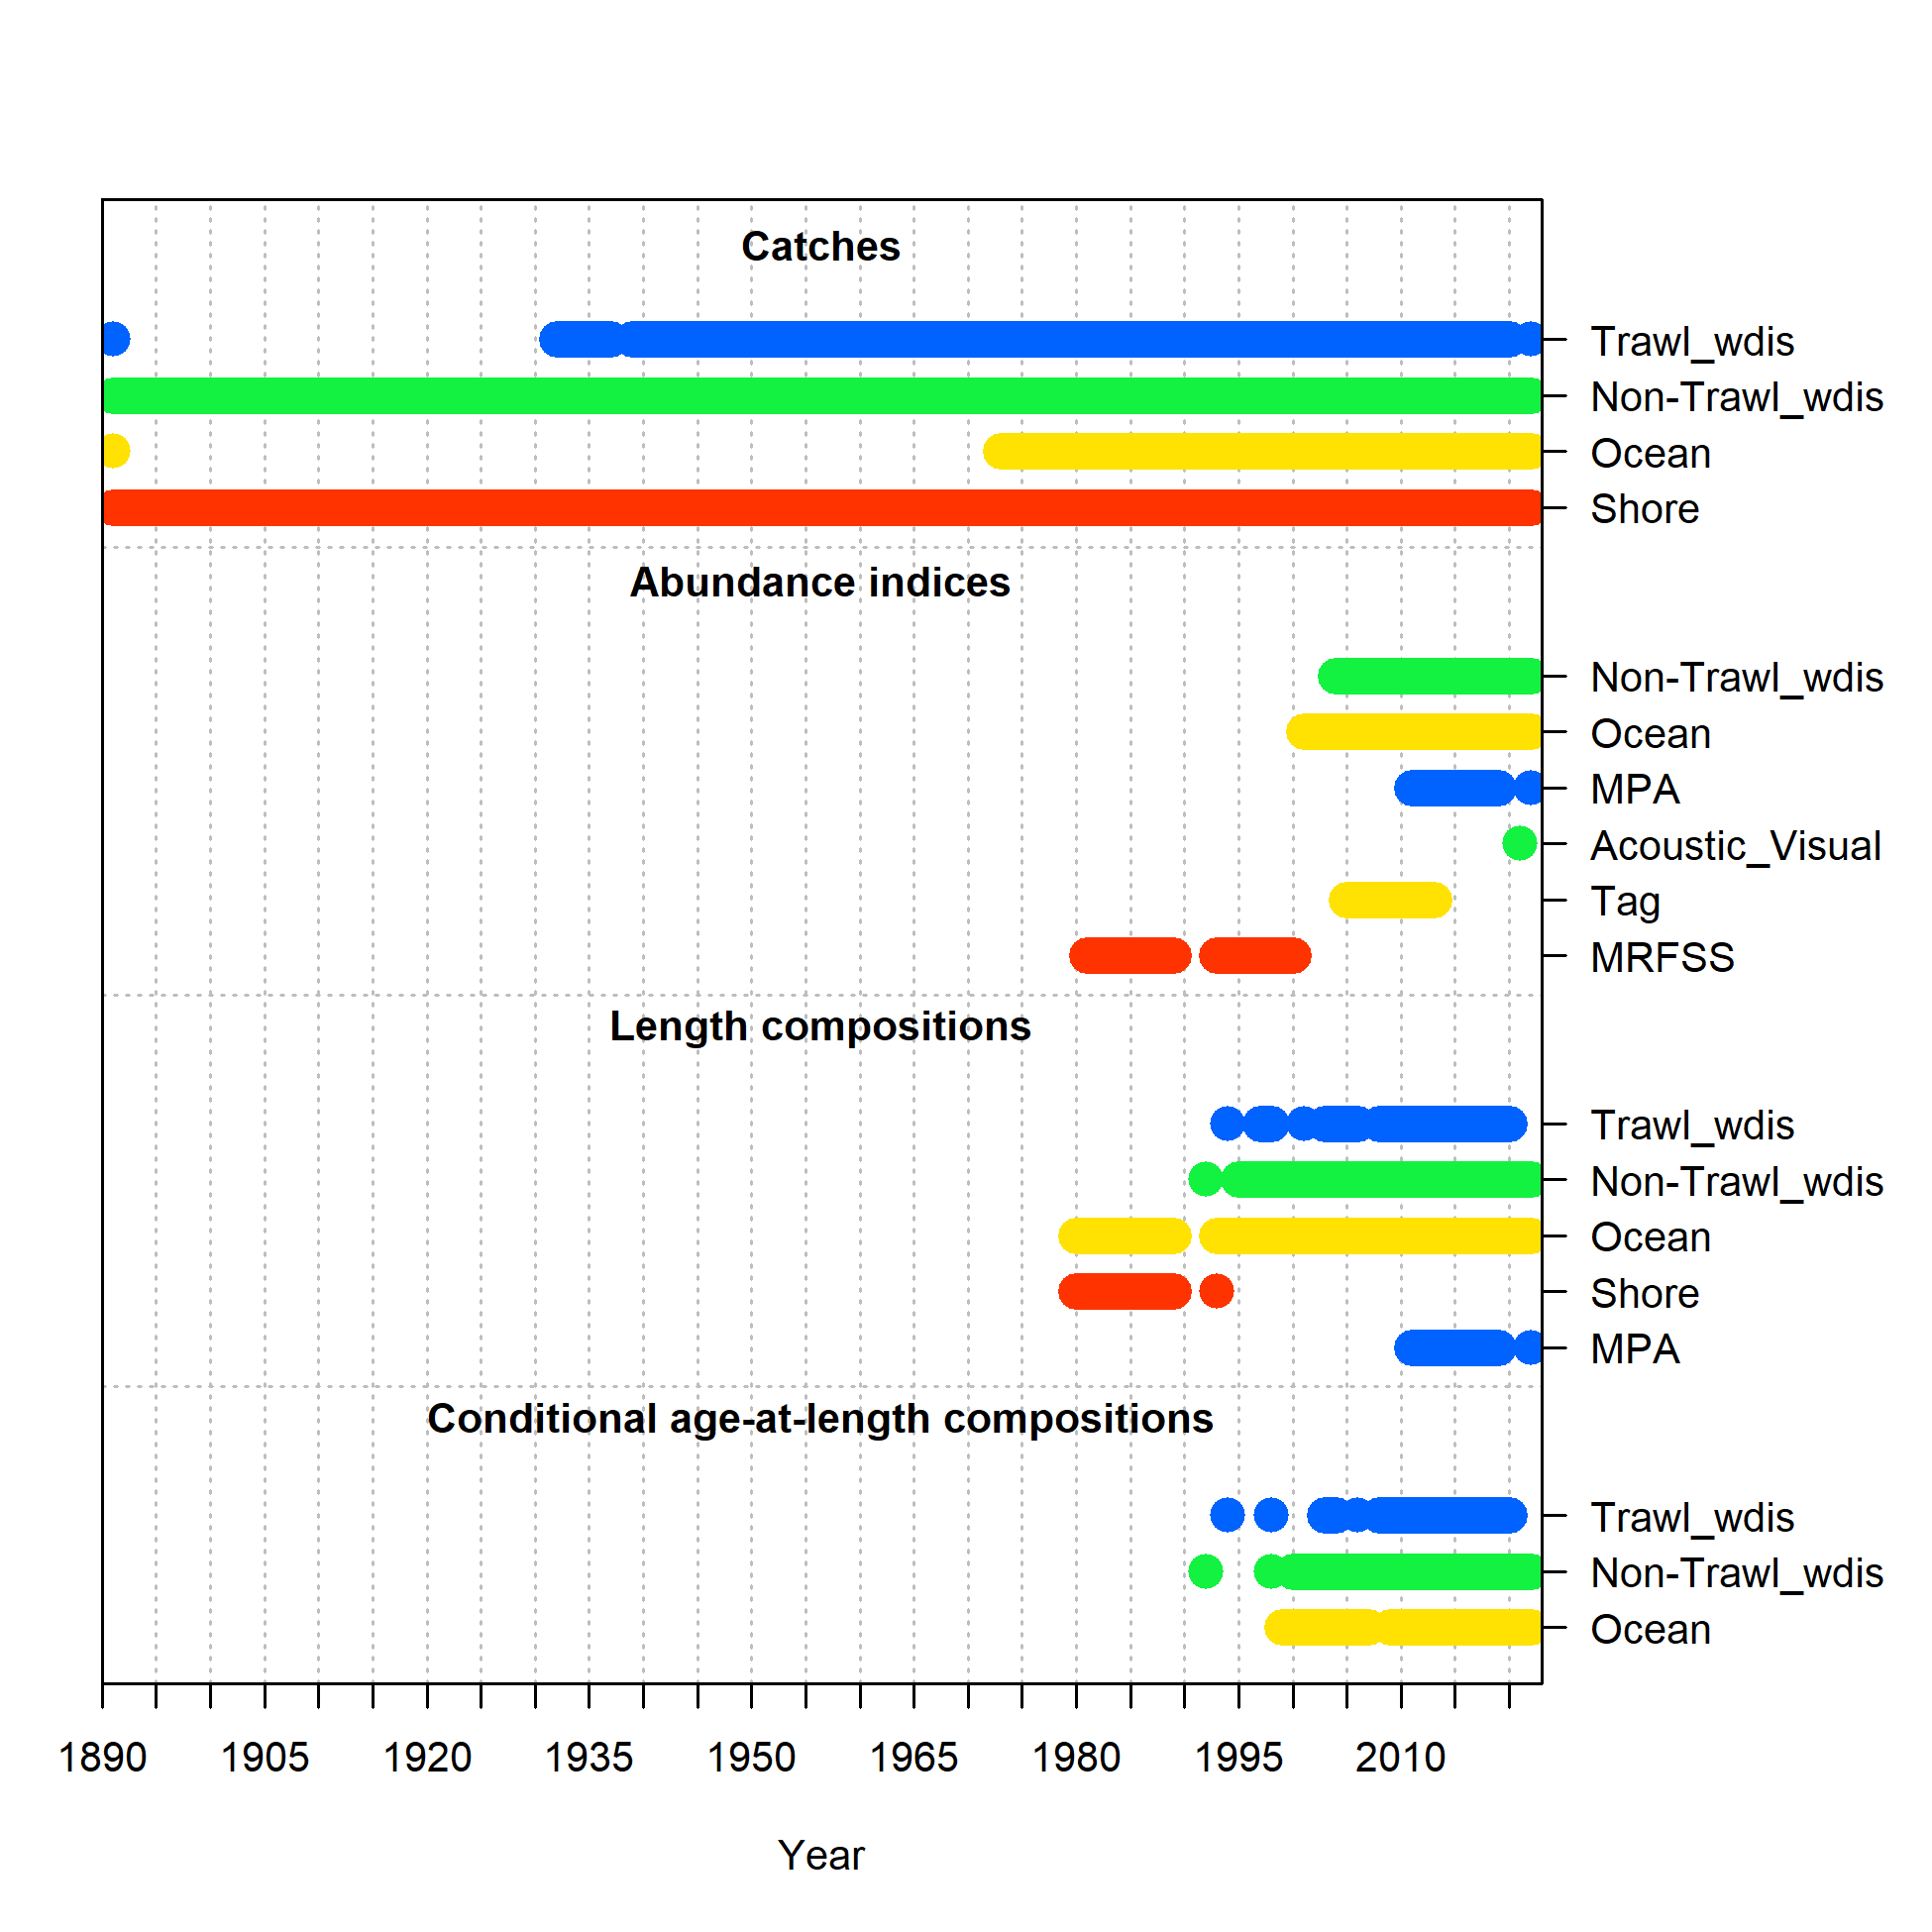
\includegraphics[width=1\textwidth,height=1\textheight]{C:/Users/Jason.Cope/Documents/Github/Sebastes_melanops_OR/Document/models/Reference model/plots/data_plot.png}
\caption{Summary of data sources used in the reference model.\label{fig:data-plot}}
\end{figure}

\begin{figure}
\centering
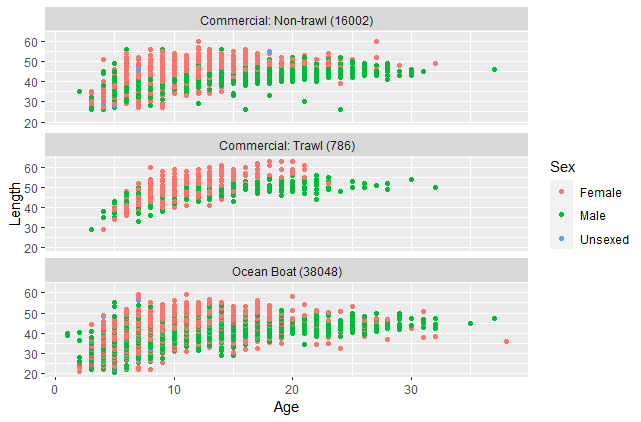
\includegraphics[width=1\textwidth,height=1\textheight]{C:/Users/Jason.Cope/Documents/Github/Sebastes_melanops_OR/Document/figures/biology_plots/OR_AG_Source_Sex.png}
\caption{Observed length-at-age by data source and sex.\label{fig:len-age-data-sex}}
\end{figure}

\begin{figure}
\centering
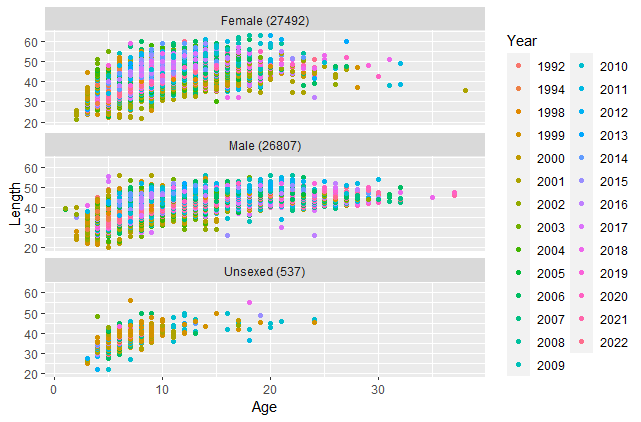
\includegraphics[width=1\textwidth,height=1\textheight]{C:/Users/Jason.Cope/Documents/Github/Sebastes_melanops_OR/Document/figures/biology_plots/OR_AG_Sex_Year.png}
\caption{Observed length-at-age by sex and year. Total samples are indicated in parentheses.\label{fig:len-age-sex-year}}
\end{figure}

\begin{figure}
\centering
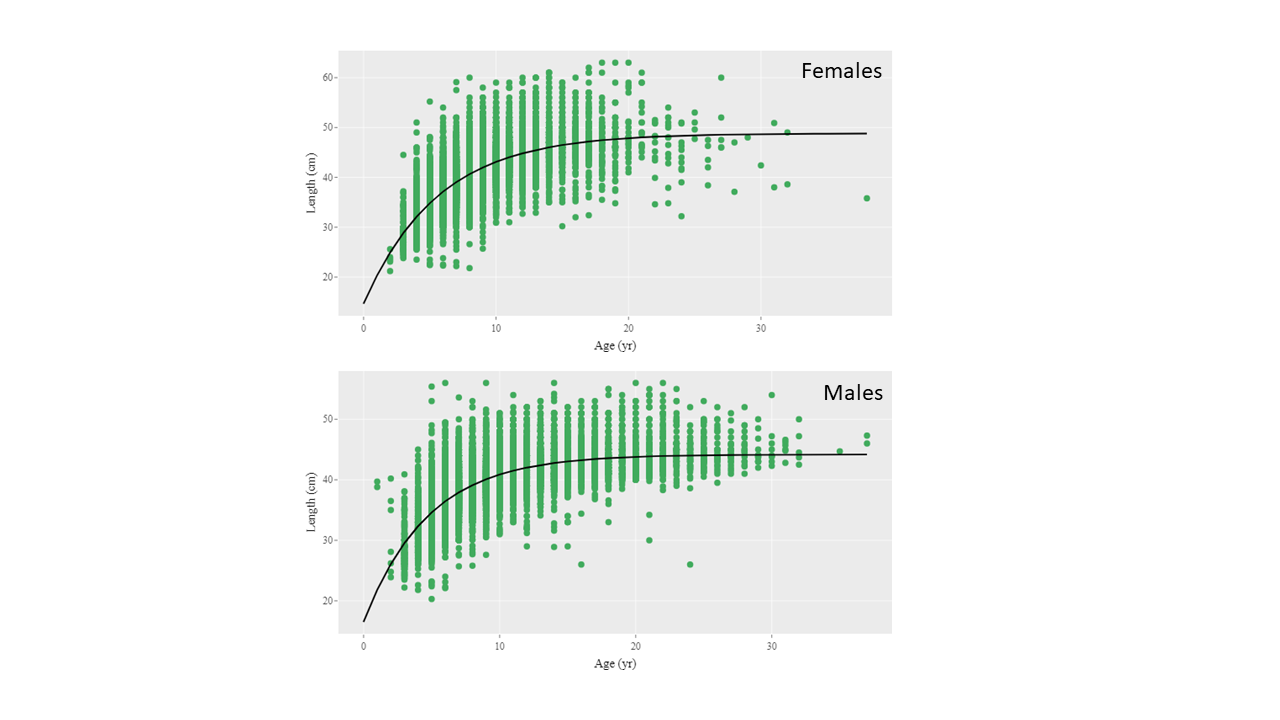
\includegraphics[width=1\textwidth,height=1\textheight]{C:/Users/Jason.Cope/Documents/Github/Sebastes_melanops_OR/Document/figures/biology_plots/OR_VBGF_fit.png}
\caption{External fits to the observed length-at-age by sex.\label{fig:len-age-fit}}
\end{figure}

\begin{figure}
\centering
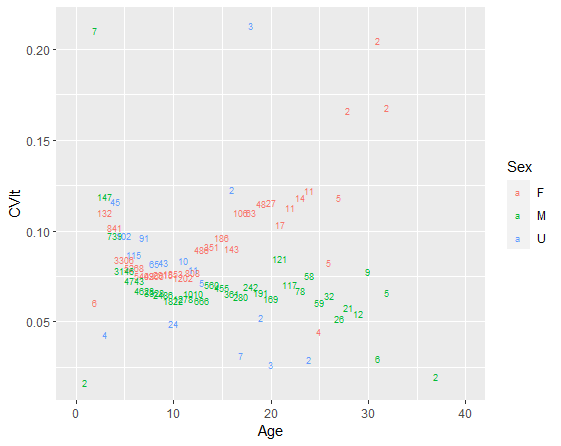
\includegraphics[width=1\textwidth,height=1\textheight]{C:/Users/Jason.Cope/Documents/Github/Sebastes_melanops_OR/Document/figures/biology_plots/OR_CV_Sex_plot.png}
\caption{Coefficient of variation of length by age by sex. Numbers indicate samples by age and colors indicate sex.\label{fig:cv-lt-age}}
\end{figure}

\begin{figure}
\centering
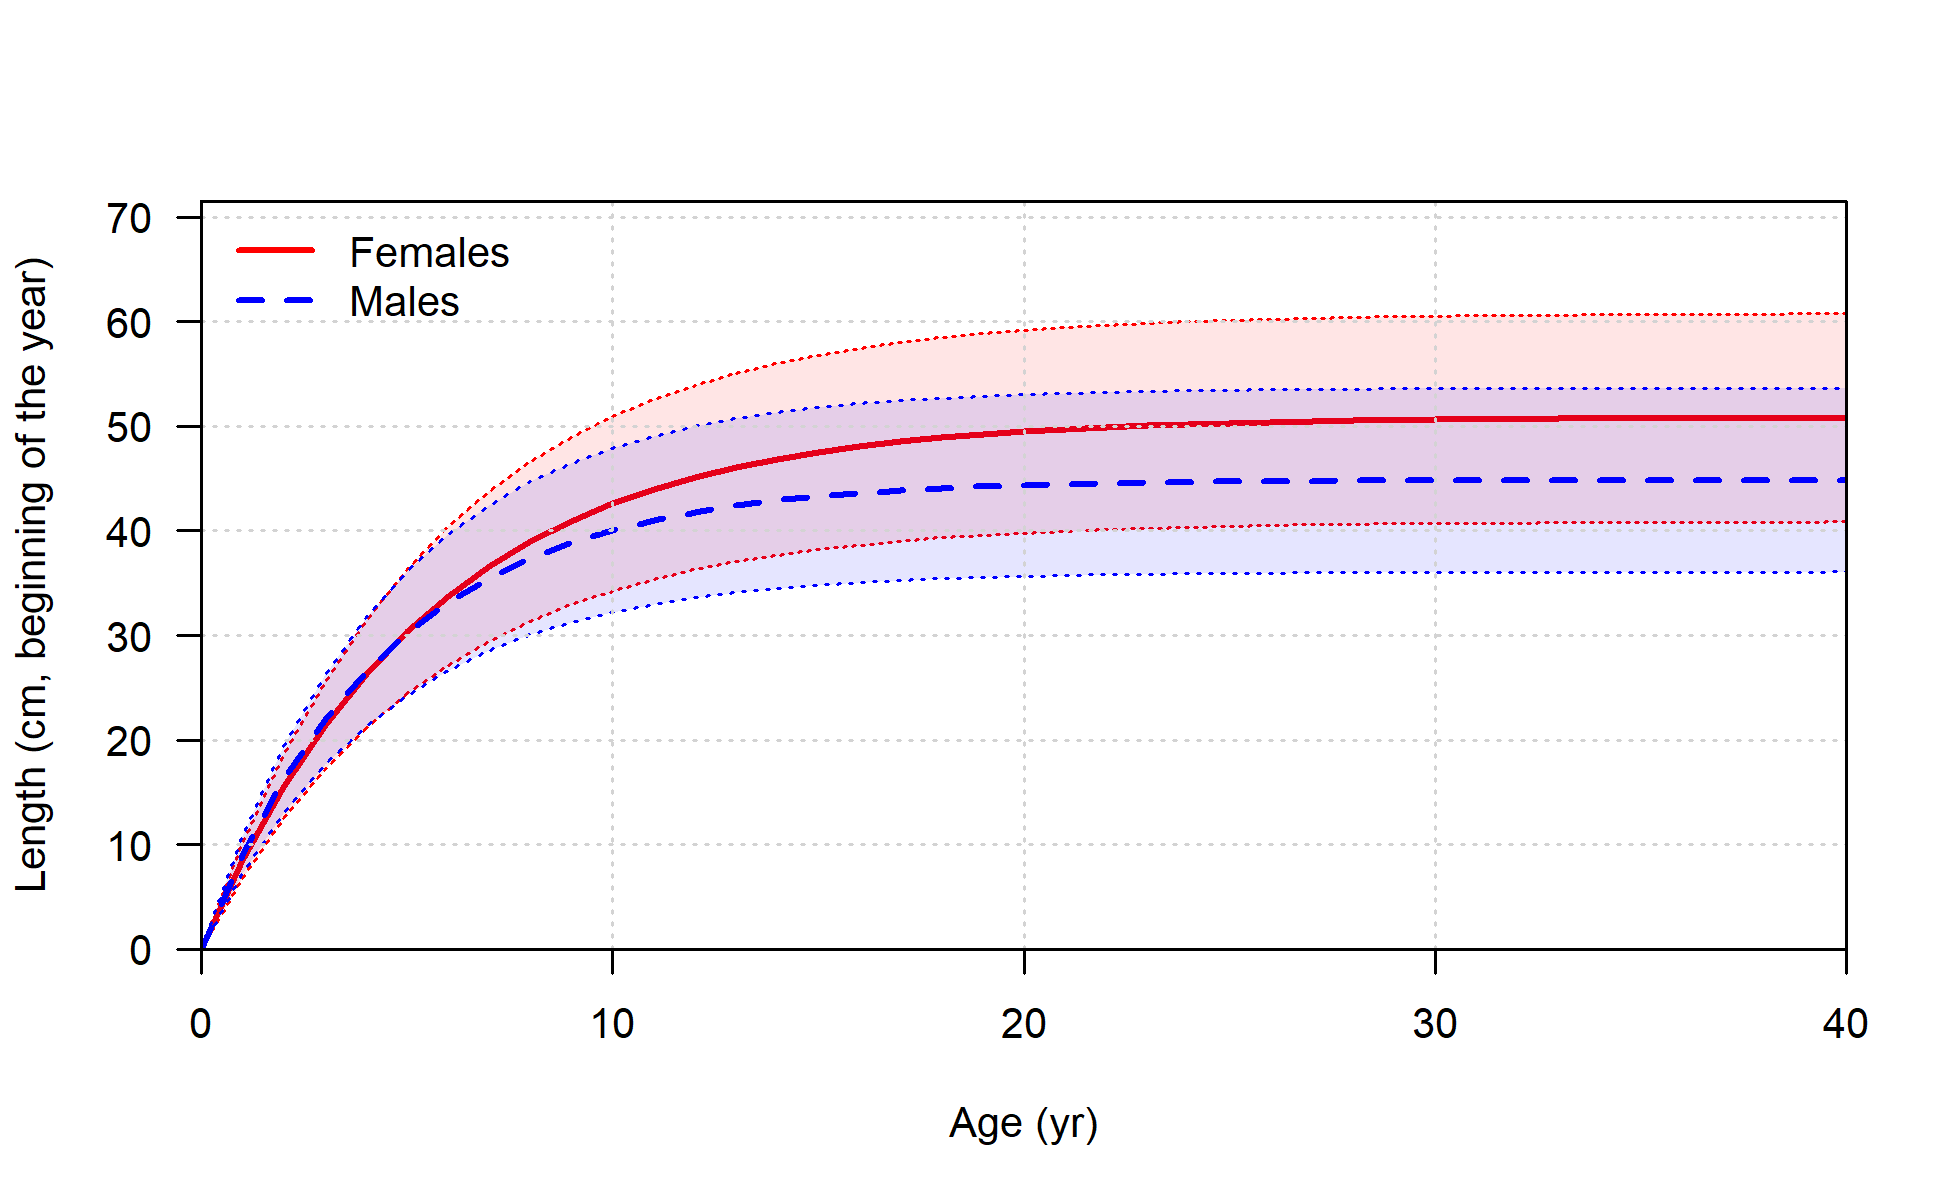
\includegraphics[width=1\textwidth,height=1\textheight]{C:/Users/Jason.Cope/Documents/Github/Sebastes_melanops_OR/Document/models/Reference model/plots/bio1_sizeatage.png}
\caption{Model estimated length-at-age. Shaded area indicates 95 percent distribution of length-at-age around the estimated growth curve.\label{fig:len-age-ss}}
\end{figure}

\clearpage

\begin{figure}
\centering
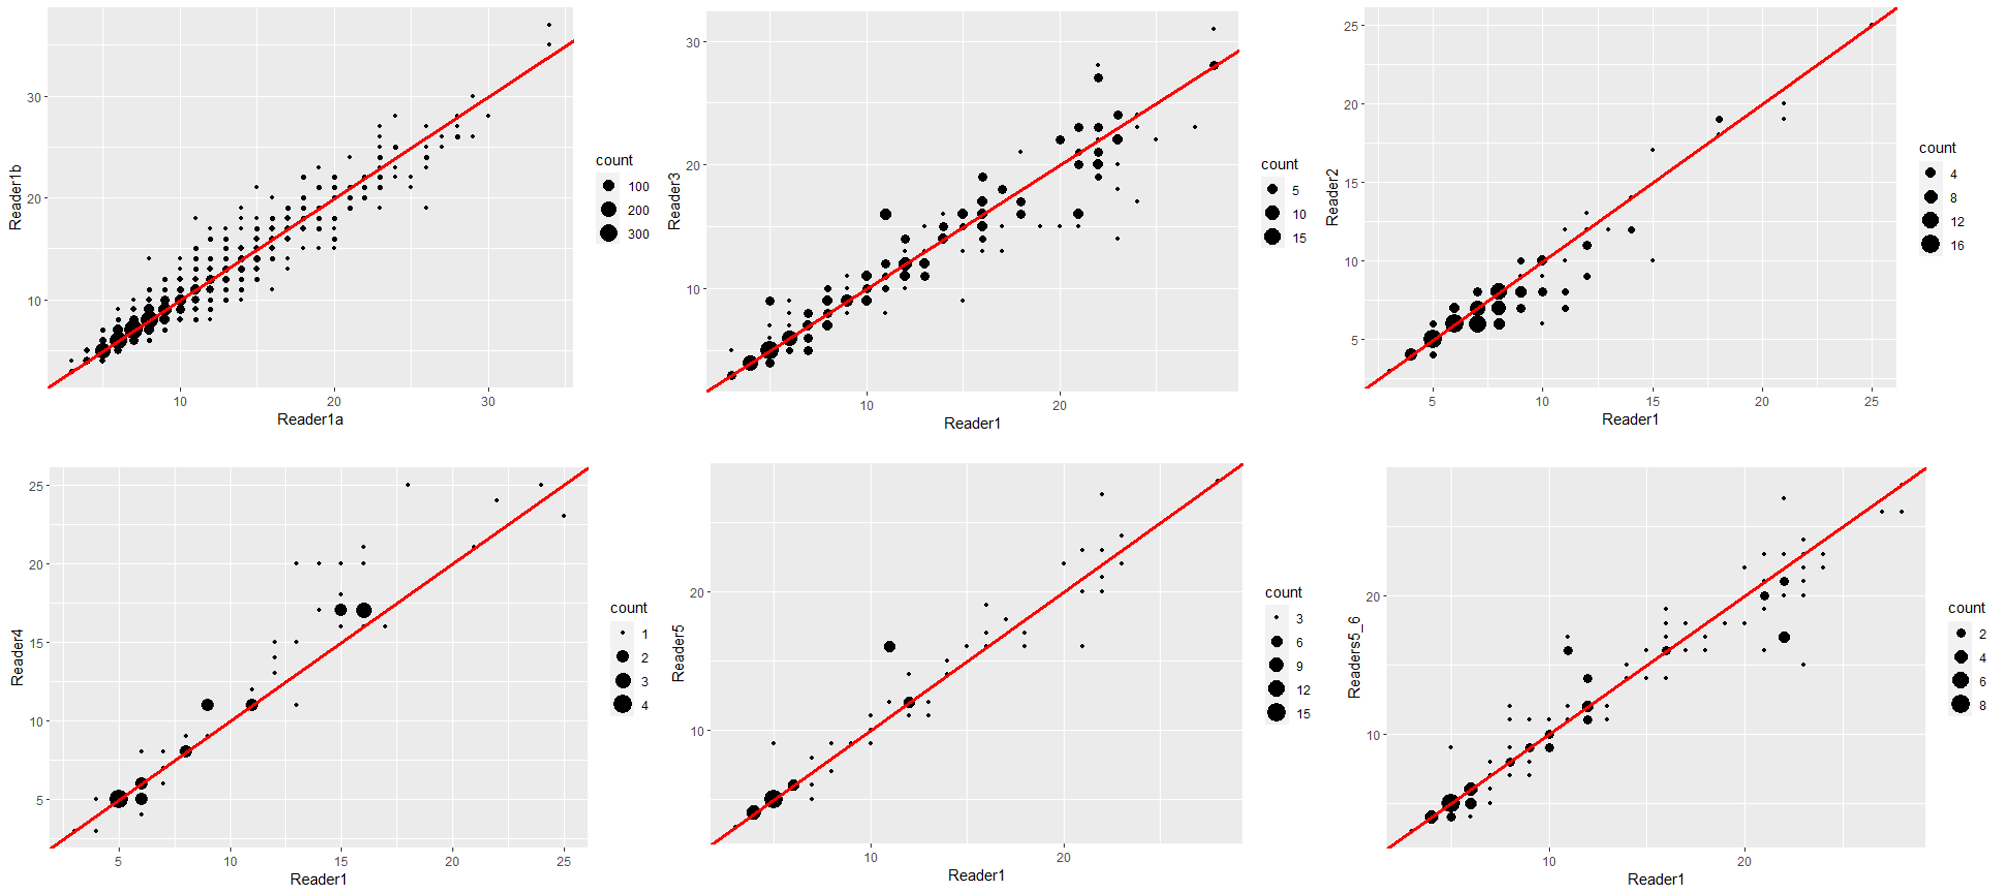
\includegraphics[width=1\textwidth,height=1\textheight]{C:/Users/Jason.Cope/Documents/Github/Sebastes_melanops_OR/Document/figures/biology_plots/Age1_1plots.png}
\caption{Ageing bias plots by reader comparisons.\label{fig:age-bias_plot}}
\end{figure}

\begin{figure}
\centering
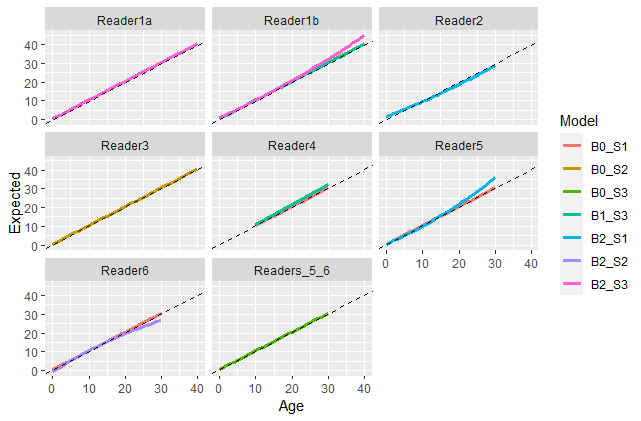
\includegraphics[width=1\textwidth,height=1\textheight]{C:/Users/Jason.Cope/Documents/Github/Sebastes_melanops_OR/Document/figures/biology_plots/OR_Reader_Bias_plot.png}
\caption{Estimated bias relationships for each considered matrix. Reader 1 is always considered unbiased. Reader 1a and 1b is an intra-reader comparison. B refers to the bias type and S refers to the imprecision type in the model selection for the ageing error matrix.\label{fig:age-error-bias}}
\end{figure}

\begin{figure}
\centering
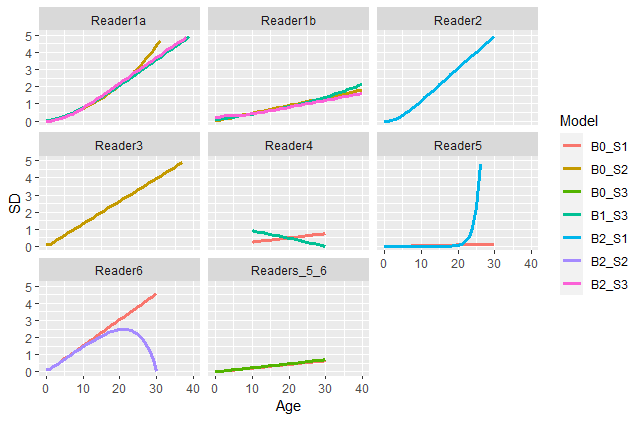
\includegraphics[width=1\textwidth,height=1\textheight]{C:/Users/Jason.Cope/Documents/Github/Sebastes_melanops_OR/Document/figures/biology_plots/OR_Reader_SD_plot.png}
\caption{Ageing error matrix standard deviation (SD) values by comparison. B refers to the bias type and S refers to the imprecision type in the model selection for the ageing error matrix.\label{fig:age-error-sd}}
\end{figure}

\begin{figure}
\centering
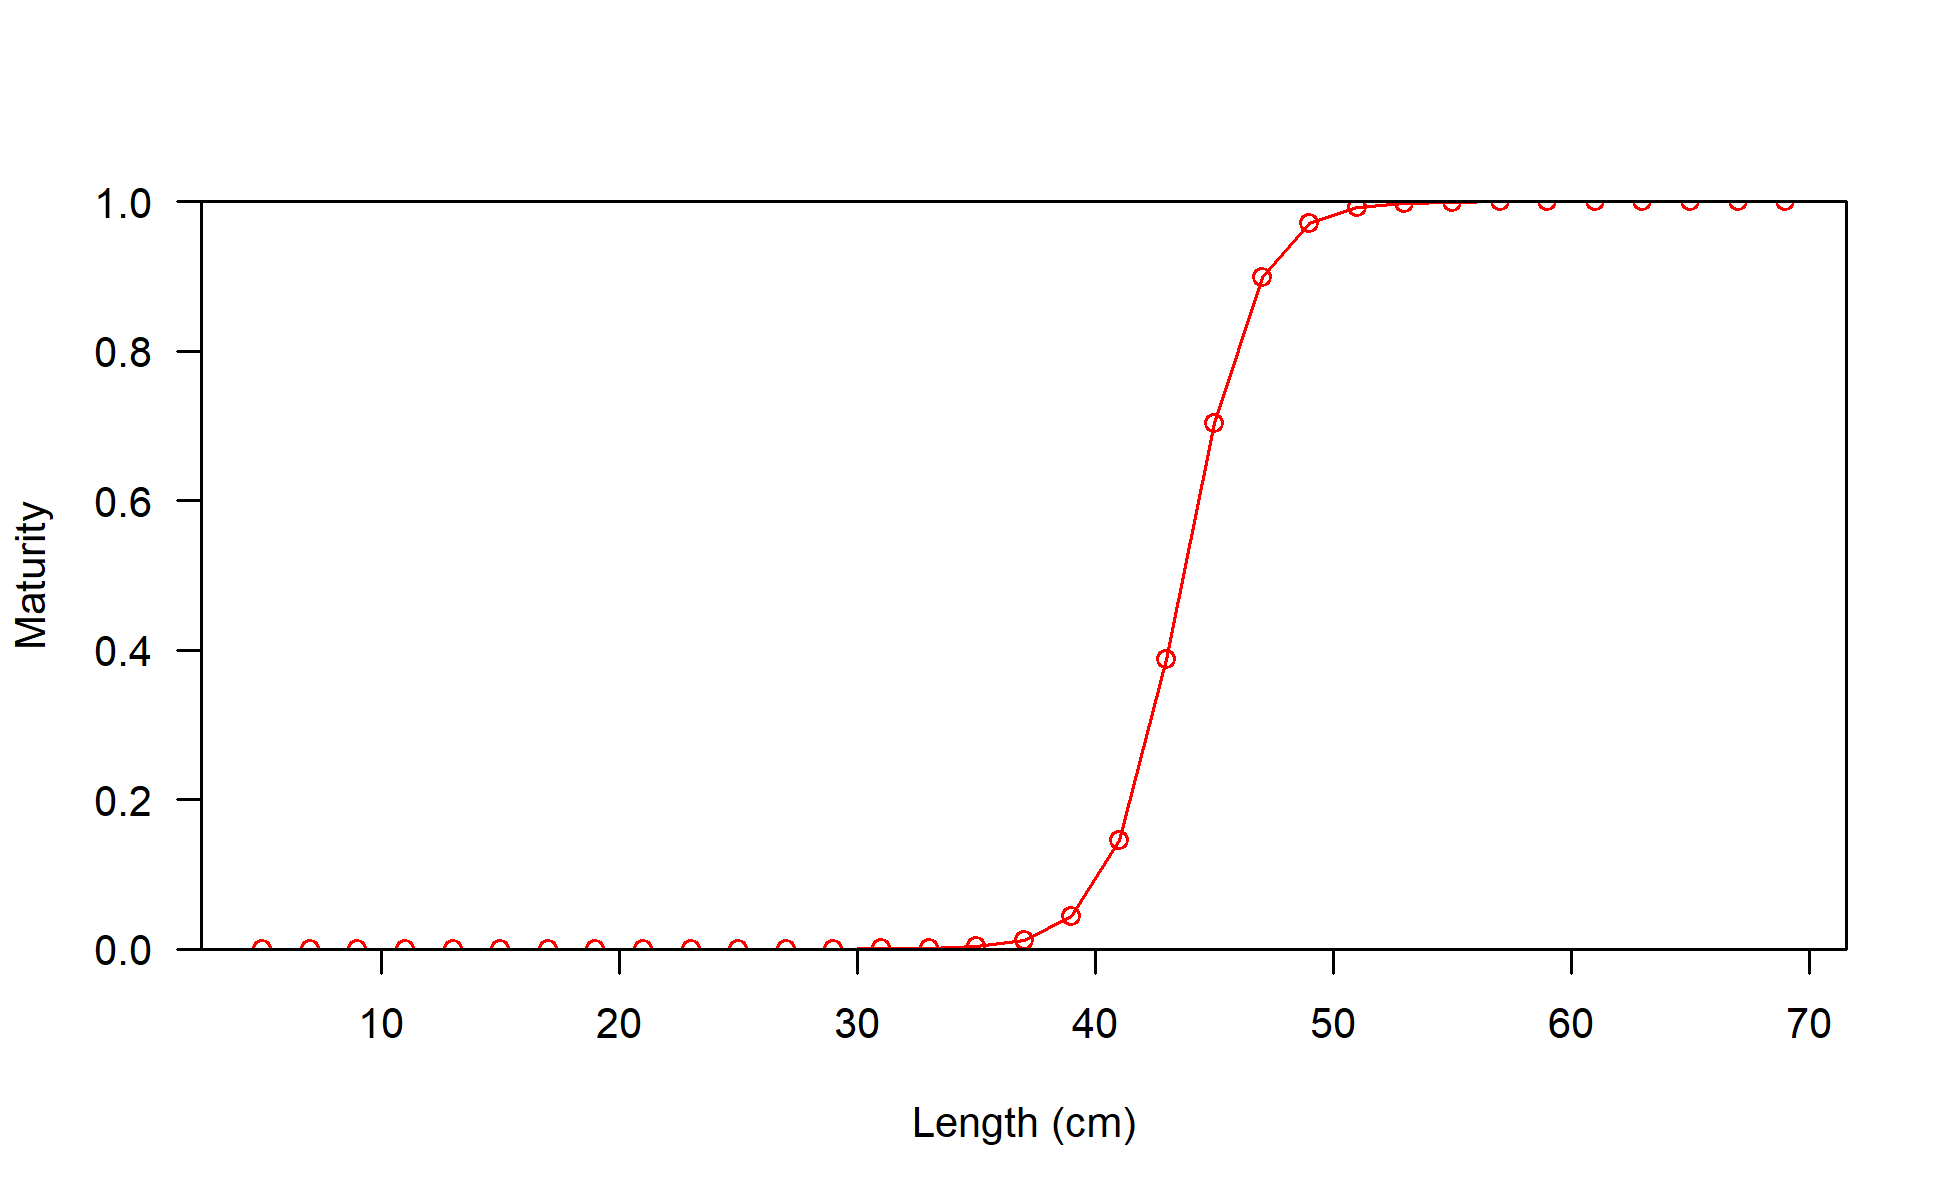
\includegraphics[width=1\textwidth,height=1\textheight]{C:/Users/Jason.Cope/Documents/Github/Sebastes_melanops_OR/Document/models/Reference model/plots/bio6_maturity.png}
\caption{Maturity as a function of length (cm).\label{fig:maturity}}
\end{figure}

\begin{figure}
\centering
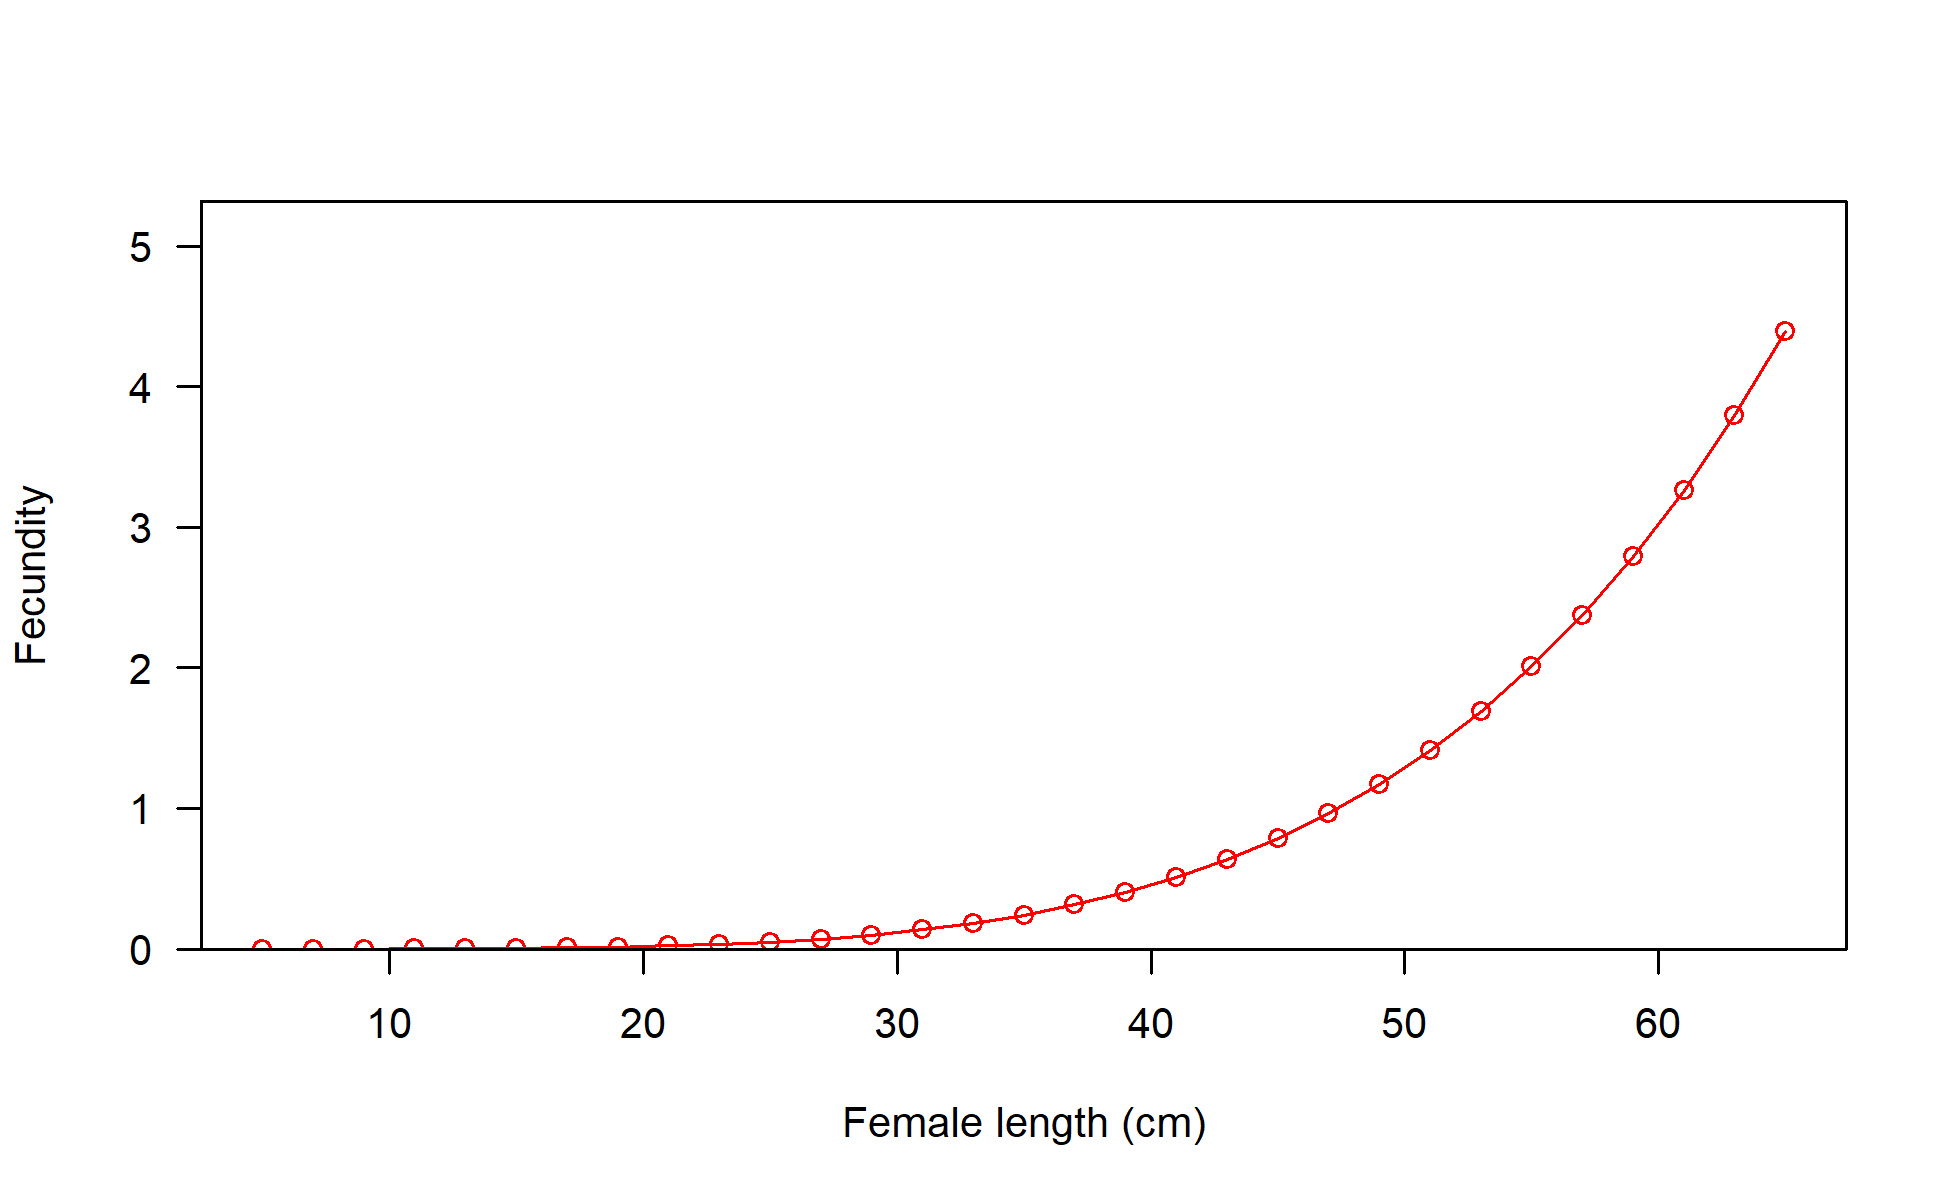
\includegraphics[width=1\textwidth,height=1\textheight]{C:/Users/Jason.Cope/Documents/Github/Sebastes_melanops_OR/Document/models/Reference model/plots/bio9_fecundity_len.png}
\caption{Fecundity (kg) as a function of length (cm).\label{fig:fecundity}}
\end{figure}

\begin{figure}
\centering
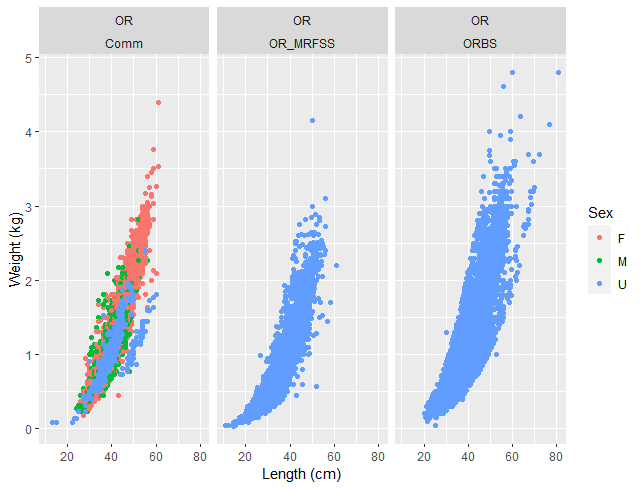
\includegraphics[width=1\textwidth,height=1\textheight]{C:/Users/Jason.Cope/Documents/Github/Sebastes_melanops_OR/Document/figures/biology_plots/LW_OR_State_Source_Sex.png}
\caption{Sex-specific length (cm)-weight (kg) data for Oregon black rockfish samples by source. MRFSS and ORBS are the ocean boat recreational fishery from early and late periods.\label{fig:len-weight-data}}
\end{figure}

\begin{figure}
\centering
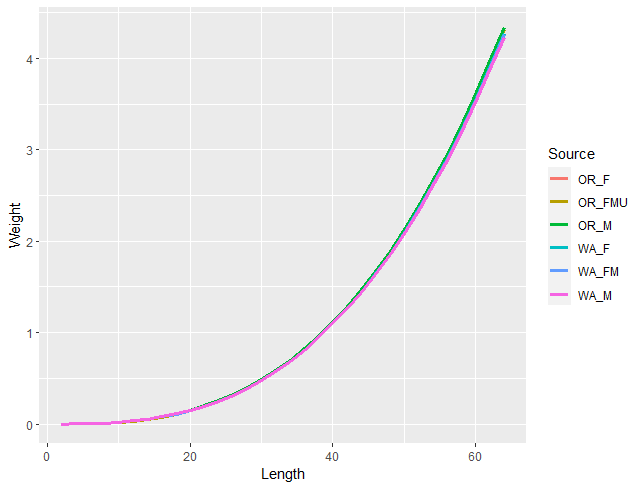
\includegraphics[width=1\textwidth,height=1\textheight]{C:/Users/Jason.Cope/Documents/Github/Sebastes_melanops_OR/Document/figures/biology_plots/LW_lines_States_Sex.png}
\caption{Sex-specific length (cm)-weight (kg) estimated power function relationships. Washington state estimate relationships are also provided for comparison.\label{fig:len-weight-or-wa}}
\end{figure}

\clearpage

\begin{figure}
\centering
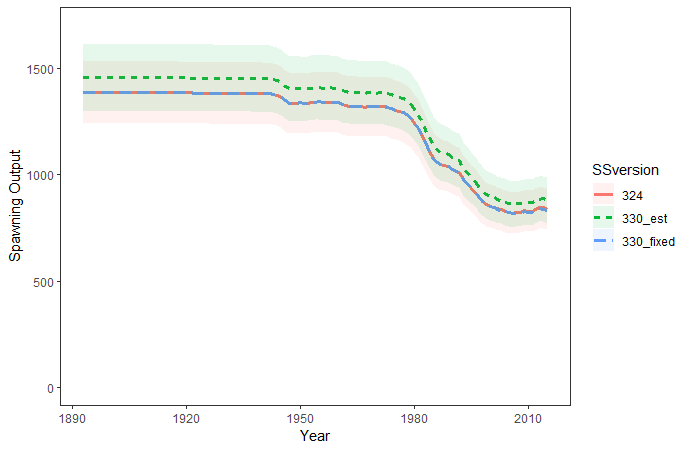
\includegraphics[width=1\textwidth,height=1\textheight]{C:/Users/Jason.Cope/Documents/Github/Sebastes_melanops_OR/Document/figures/Bridge/OR_SB_comp_plot.png}
\caption{Comparison of spawning output for black rockfish in waters off of Oregon between Stock Synthesis versions 3.24 and 3.30. Uncertainty envelops are 95\% confidence intervals.\label{fig:ssb_bridge_comps}}
\end{figure}

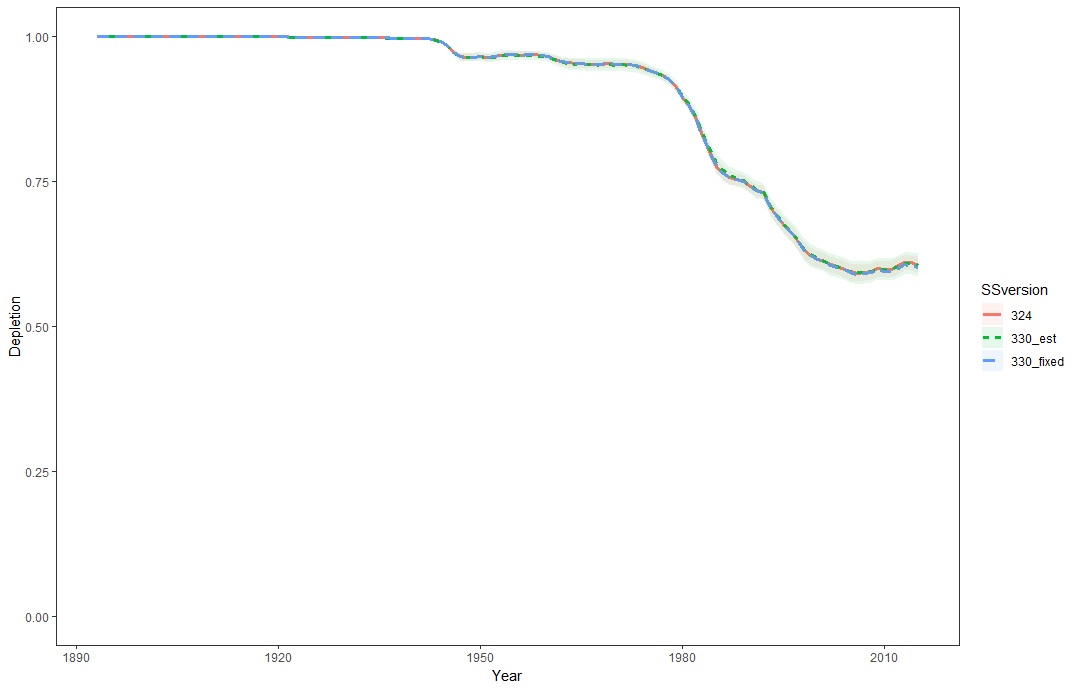
\includegraphics[width=1\textwidth,height=1\textheight]{C:/Users/Jason.Cope/Documents/Github/Sebastes_melanops_OR/Document/figures/Bridge/OR_Dep_comp_plot.png} \clearpage

\begin{figure}
\centering
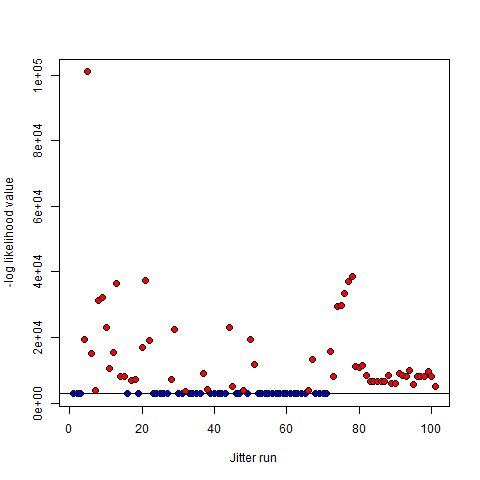
\includegraphics[width=1\textwidth,height=1\textheight]{C:/Users/Jason.Cope/Documents/Github/Sebastes_melanops_OR/Document/figures/modconverge/jitterplot.png}
\caption{Jitter runs for the black rockfish reference model, with jitter run number on the x-axis and -log likelihood value on the y-axis. Blue dot are models that match the likelihood value of the reference model, while red dots deviate from the reference model. All red dots are above the blue dots, indicating no better fit to the reference model was found.\label{fig:jitter}}
\end{figure}

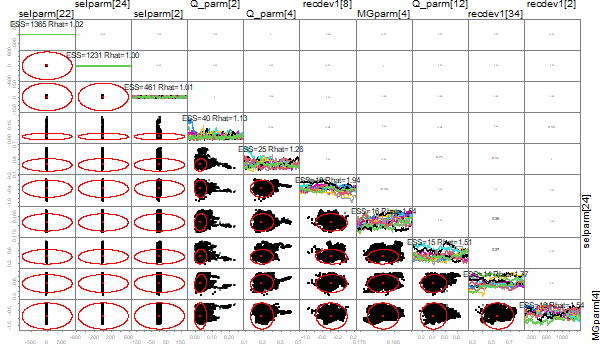
\includegraphics[width=1\textwidth,height=1\textheight]{C:/Users/Jason.Cope/Documents/Github/Sebastes_melanops_OR/Document/figures/modconverge/pairs_plot_fast.png} \clearpage

\begin{figure}
\centering
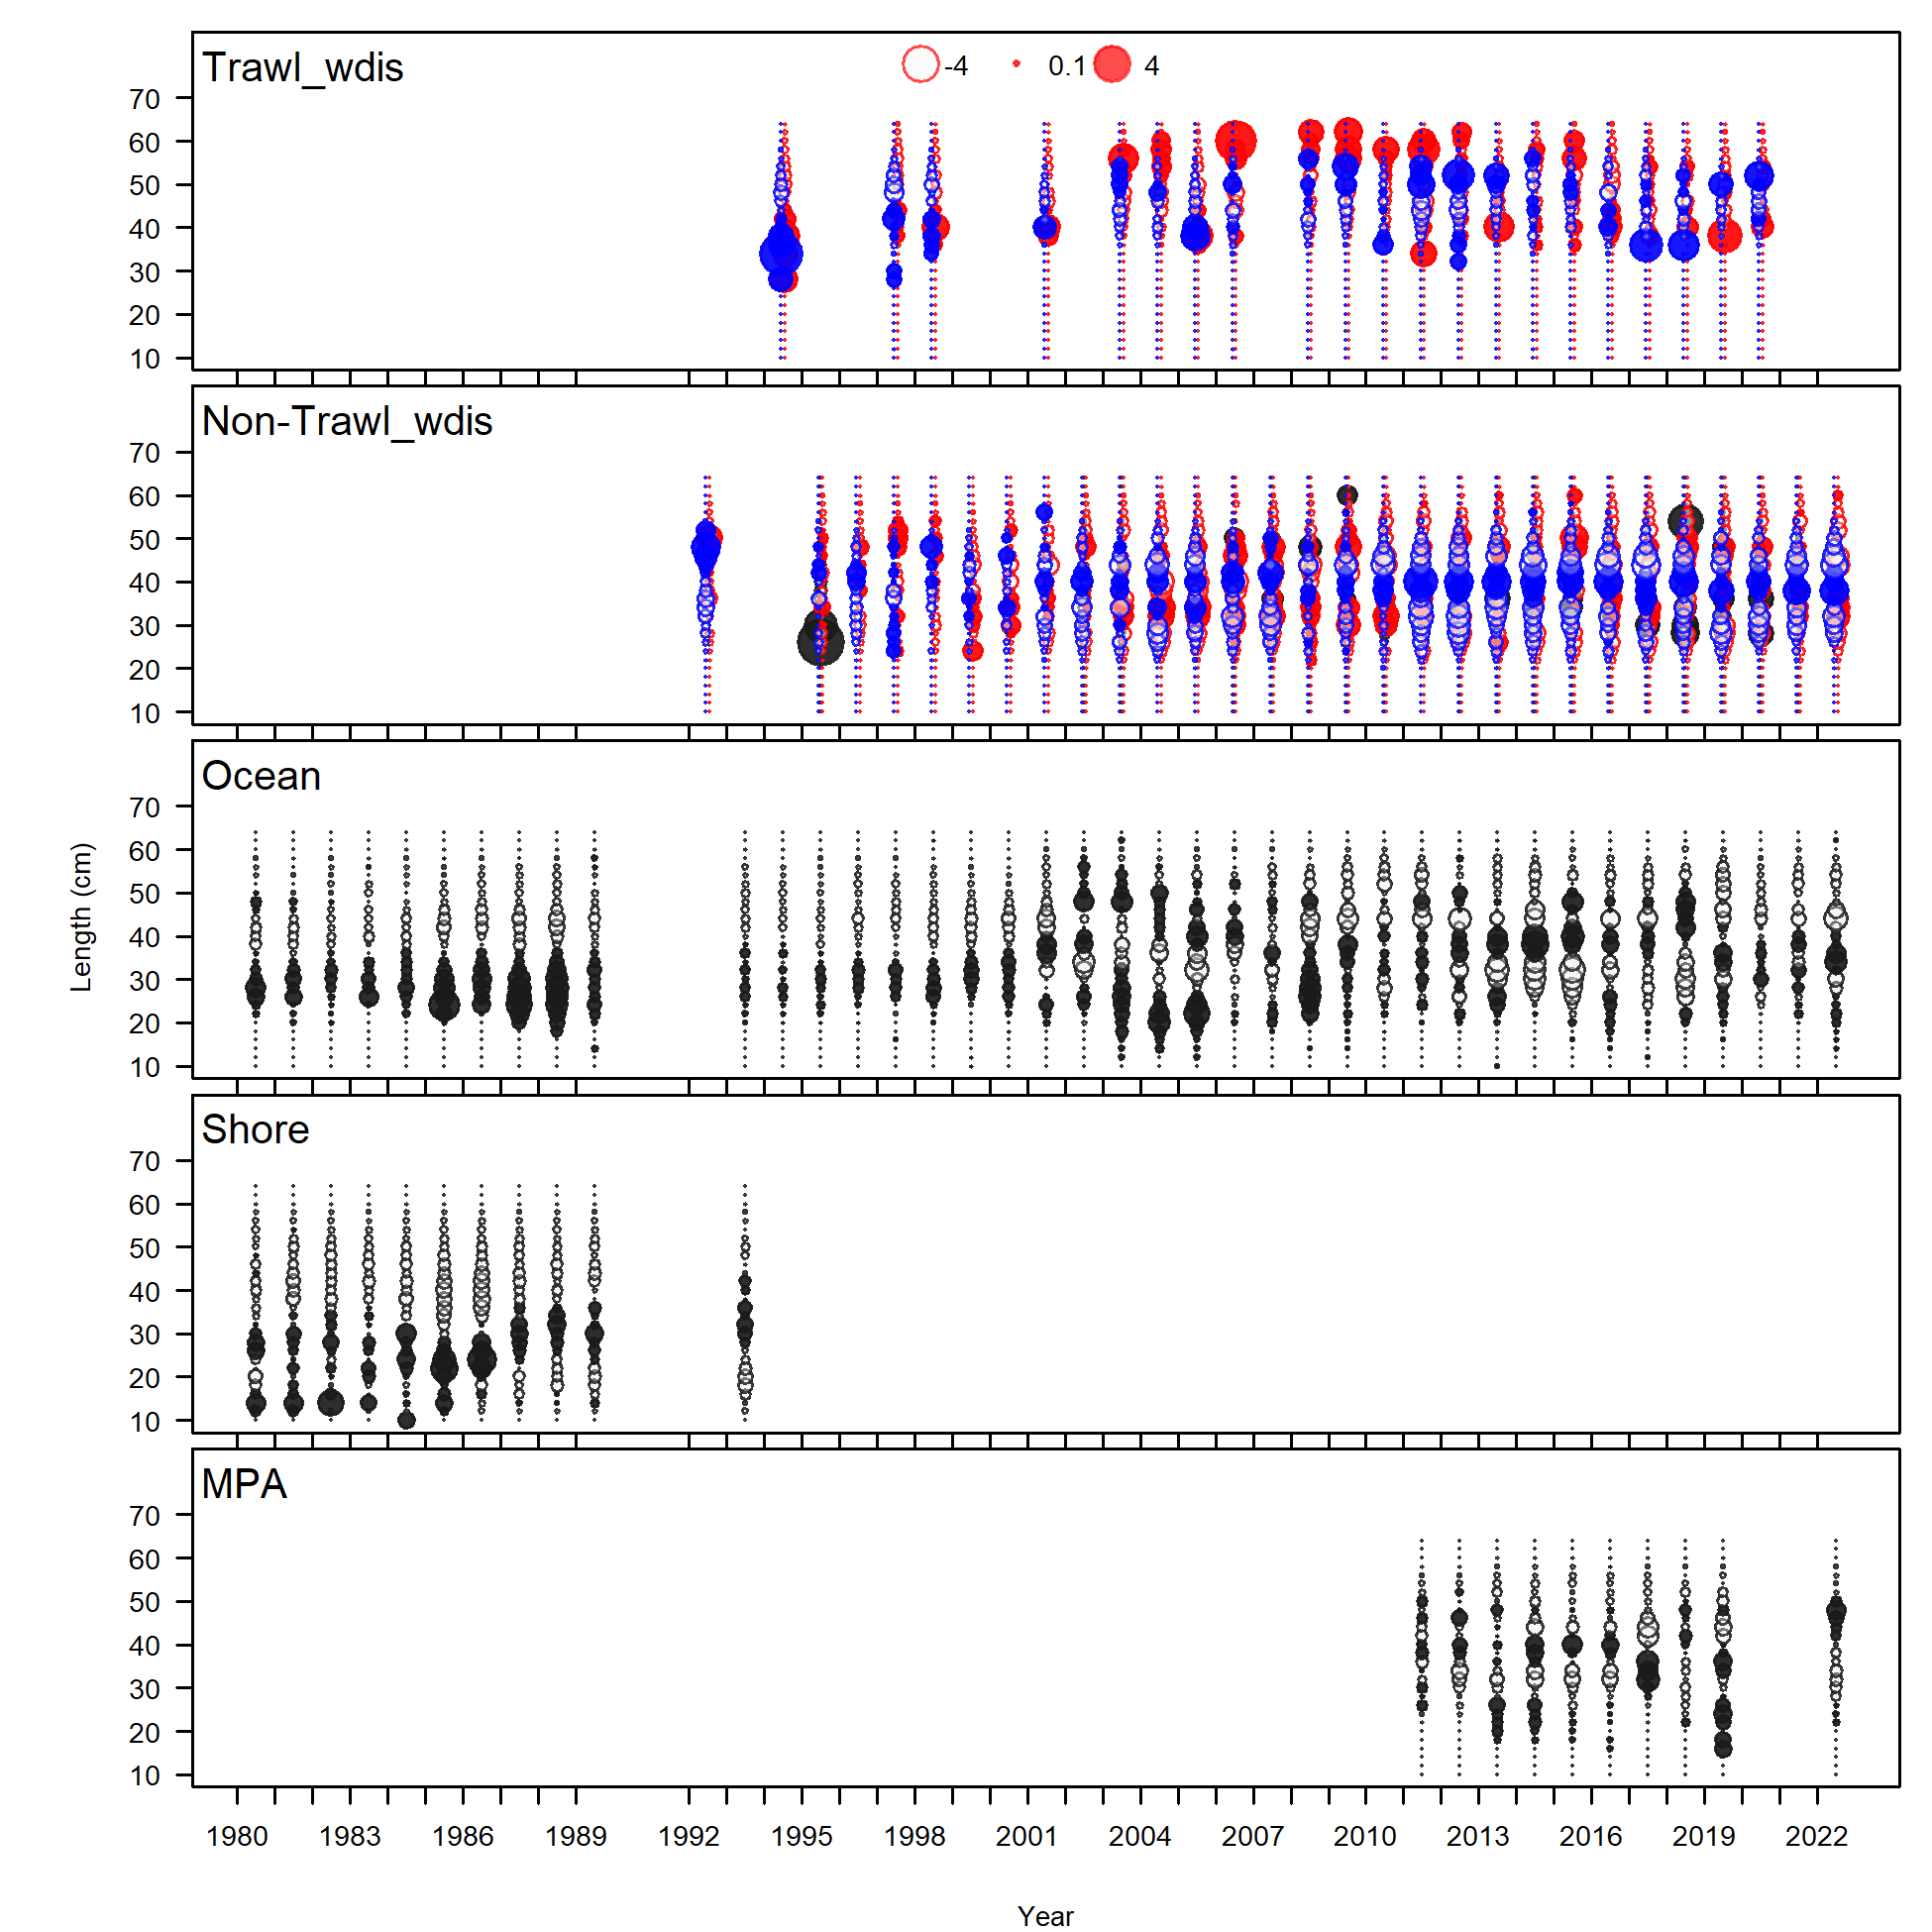
\includegraphics[width=1\textwidth,height=1\textheight]{C:/Users/Jason.Cope/Documents/Github/Sebastes_melanops_OR/Document/models/Reference model/plots/comp_lenfit__multi-fleet_comparison.png}
\caption{Pearson residuals for each fishing fleet and the MPA survey. Closed bubble are positive residuals (observed \textgreater{} expected) and open bubbles are negative residuals (observed \textless{} expected).\label{fig:lt-pearson-resids}}
\end{figure}

\begin{figure}
\centering
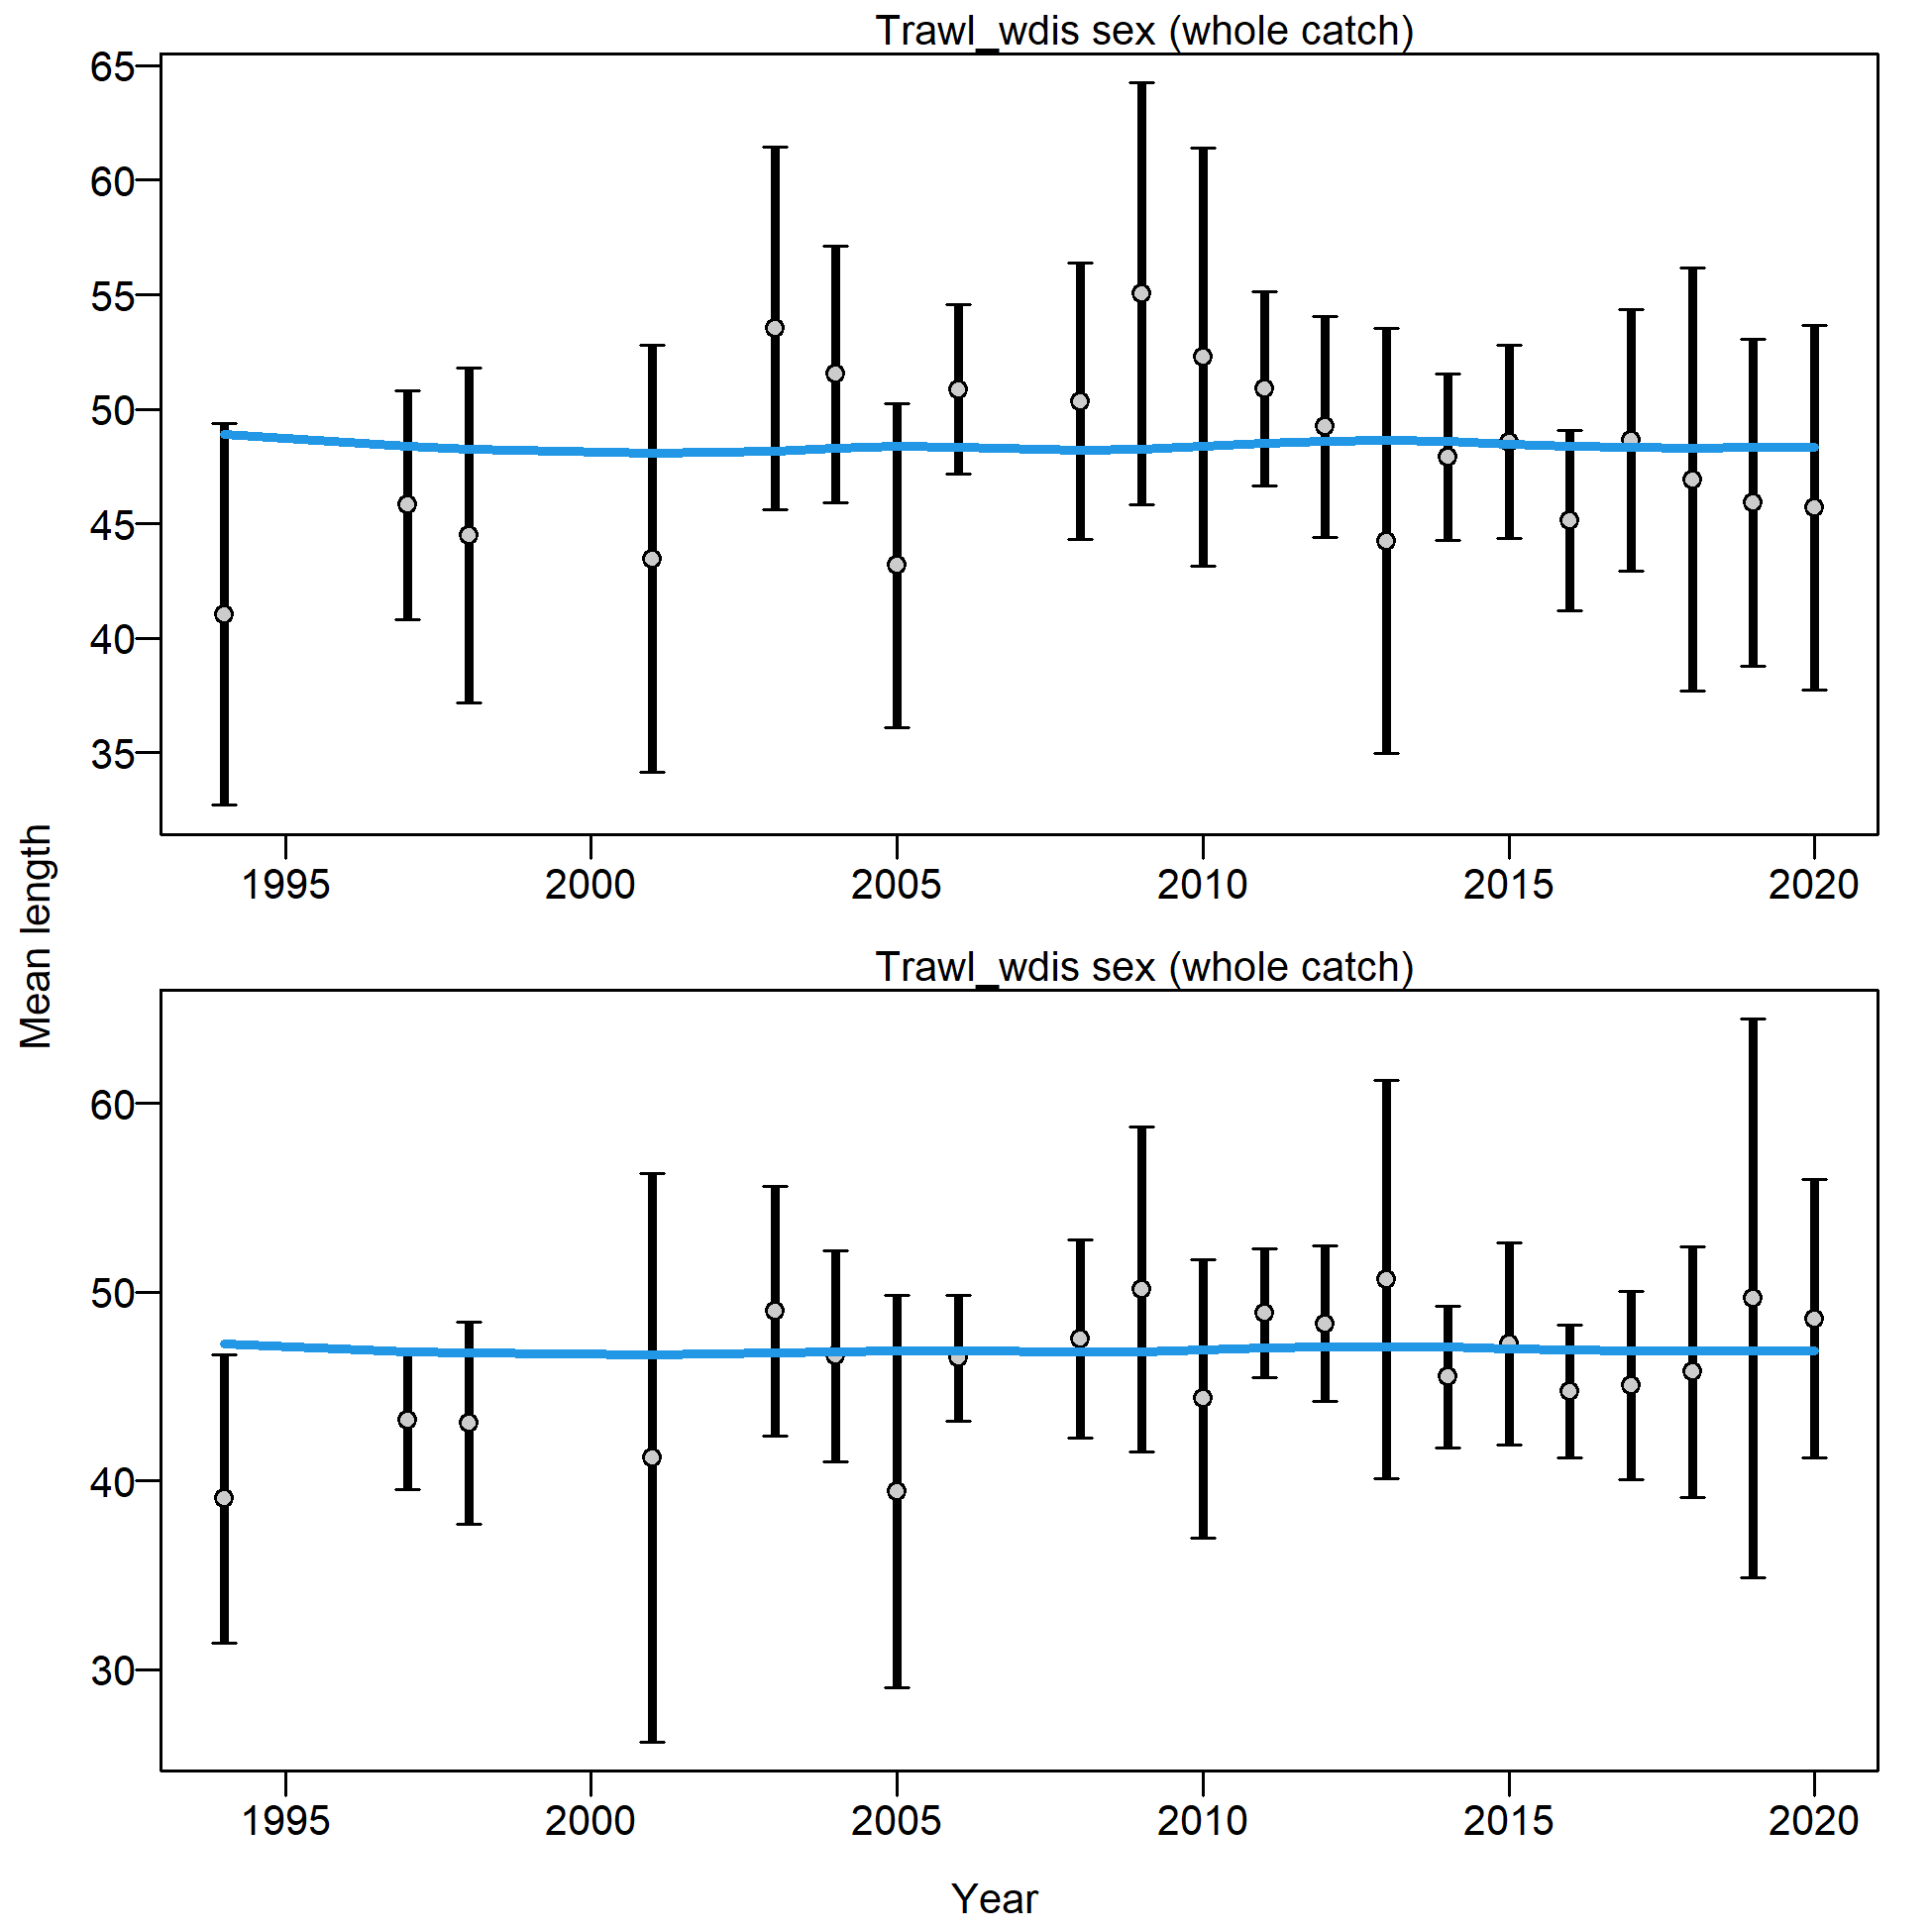
\includegraphics[width=1\textwidth,height=1\textheight]{C:/Users/Jason.Cope/Documents/Github/Sebastes_melanops_OR/Document/models/Reference model/plots/comp_lenfit_data_weighting_TA1.8_Trawl_wdis.png}
\caption{Mean length (cm) index from the trawl fishery with 95 percent confidence intervals based on sample sizes and data weighting.\label{fig:trawl-mean-len-fit}}
\end{figure}

\begin{figure}
\centering
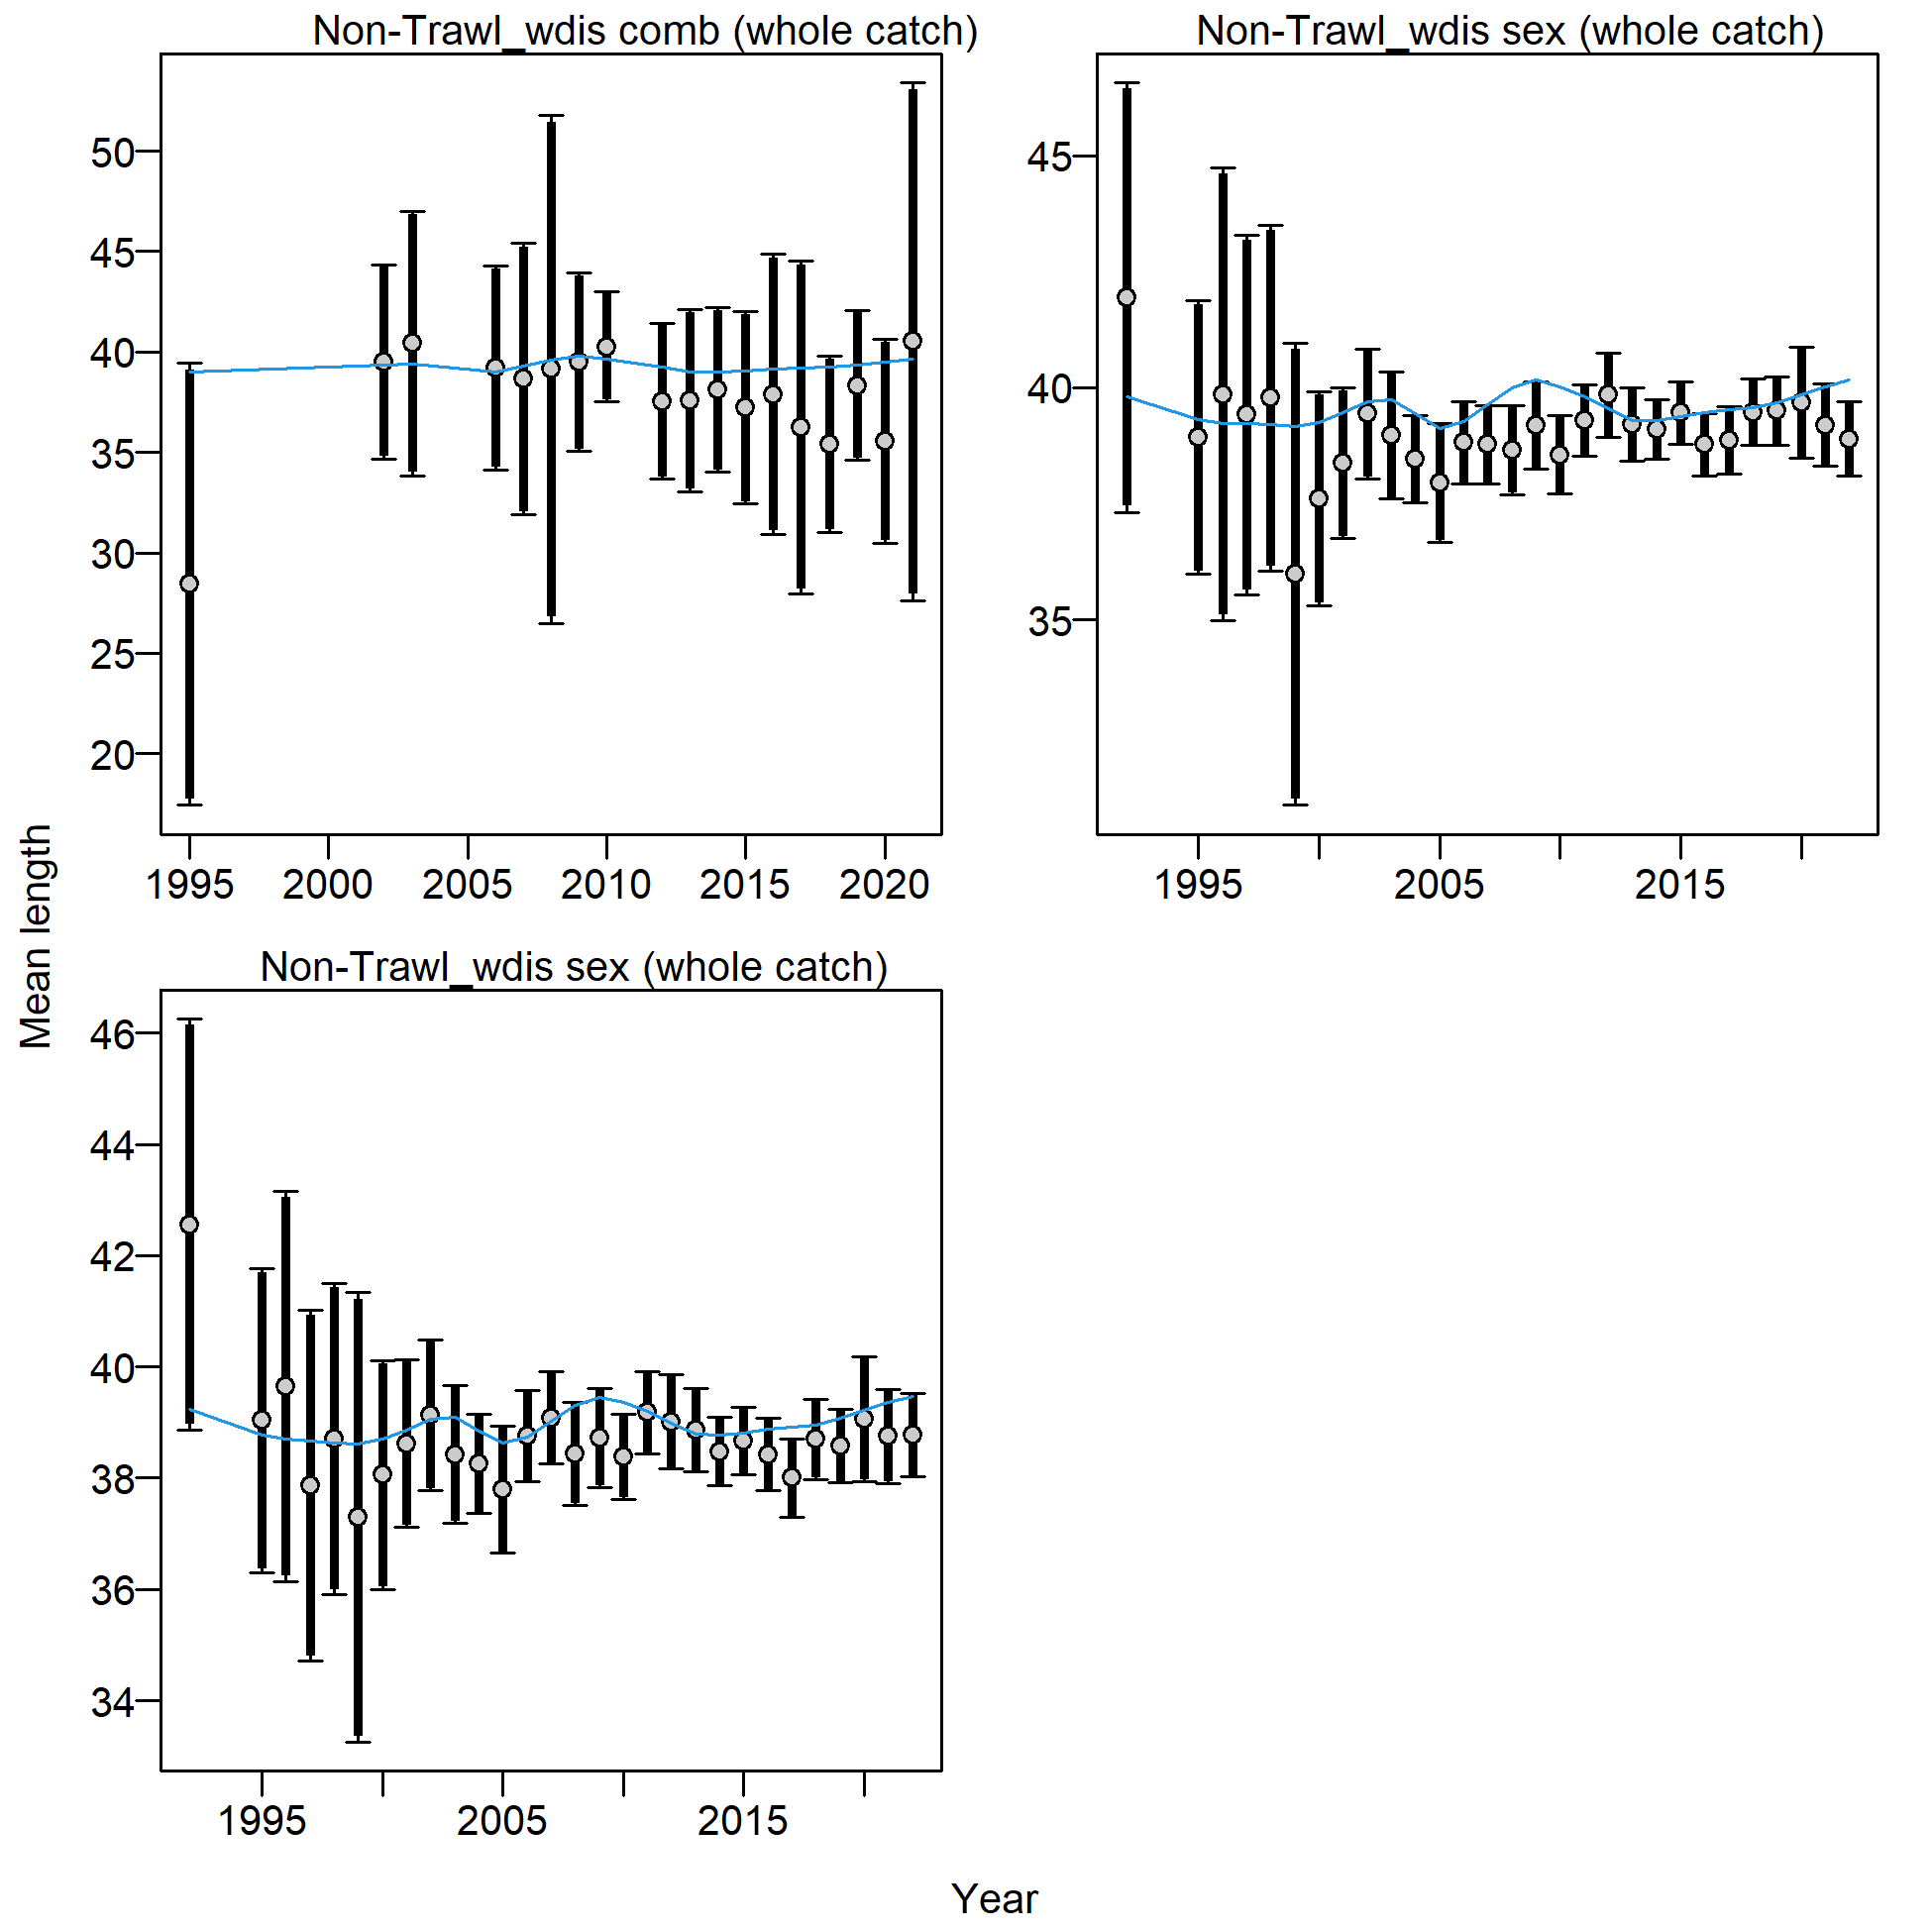
\includegraphics[width=1\textwidth,height=1\textheight]{C:/Users/Jason.Cope/Documents/Github/Sebastes_melanops_OR/Document/models/Reference model/plots/comp_lenfit_data_weighting_TA1.8_Non-Trawl_wdis.png}
\caption{Mean length (cm) index from the recreational fishery with 95 percent confidence intervals based on sample sizes and data weighting.\label{fig:nontrawl-mean-len-fit}}
\end{figure}

\begin{figure}
\centering
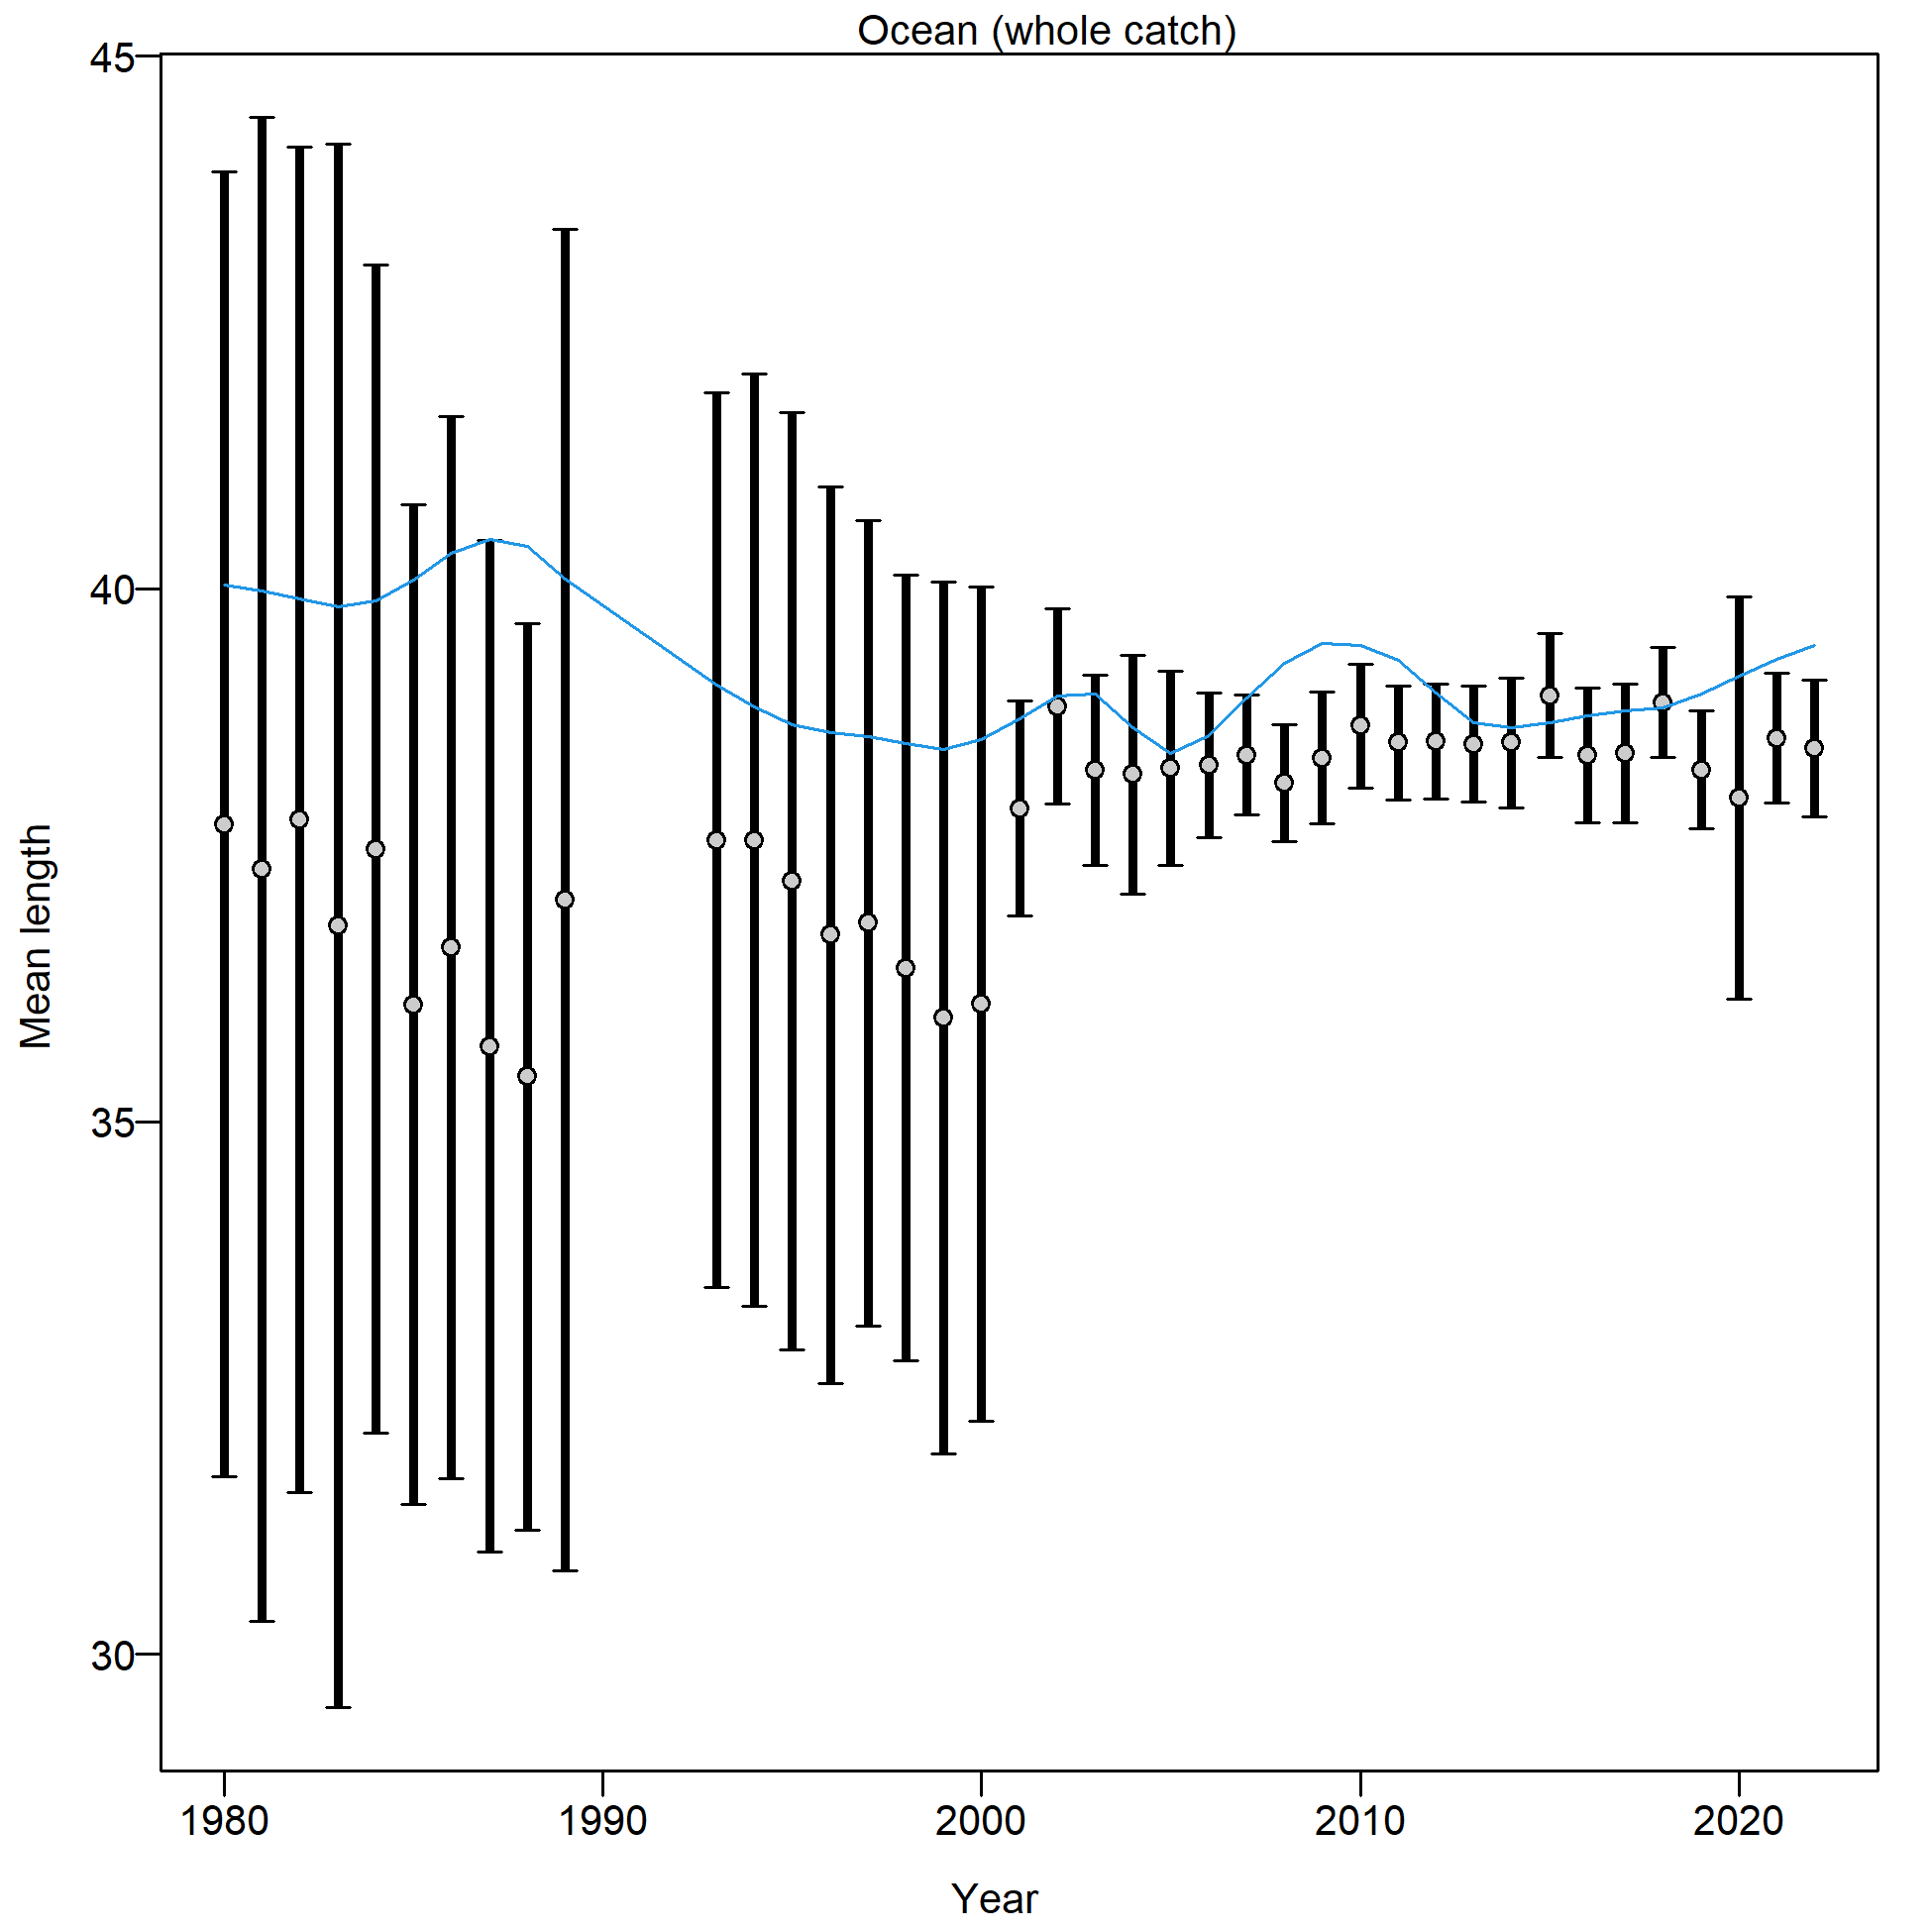
\includegraphics[width=1\textwidth,height=1\textheight]{C:/Users/Jason.Cope/Documents/Github/Sebastes_melanops_OR/Document/models/Reference model/plots/comp_lenfit_data_weighting_TA1.8_Ocean.png}
\caption{Mean length (cm) index from the recreational ocean boat fishery with 95 percent confidence intervals based on sample sizes and data weighting.\label{fig:ocean-mean-len-fit}}
\end{figure}

\begin{figure}
\centering
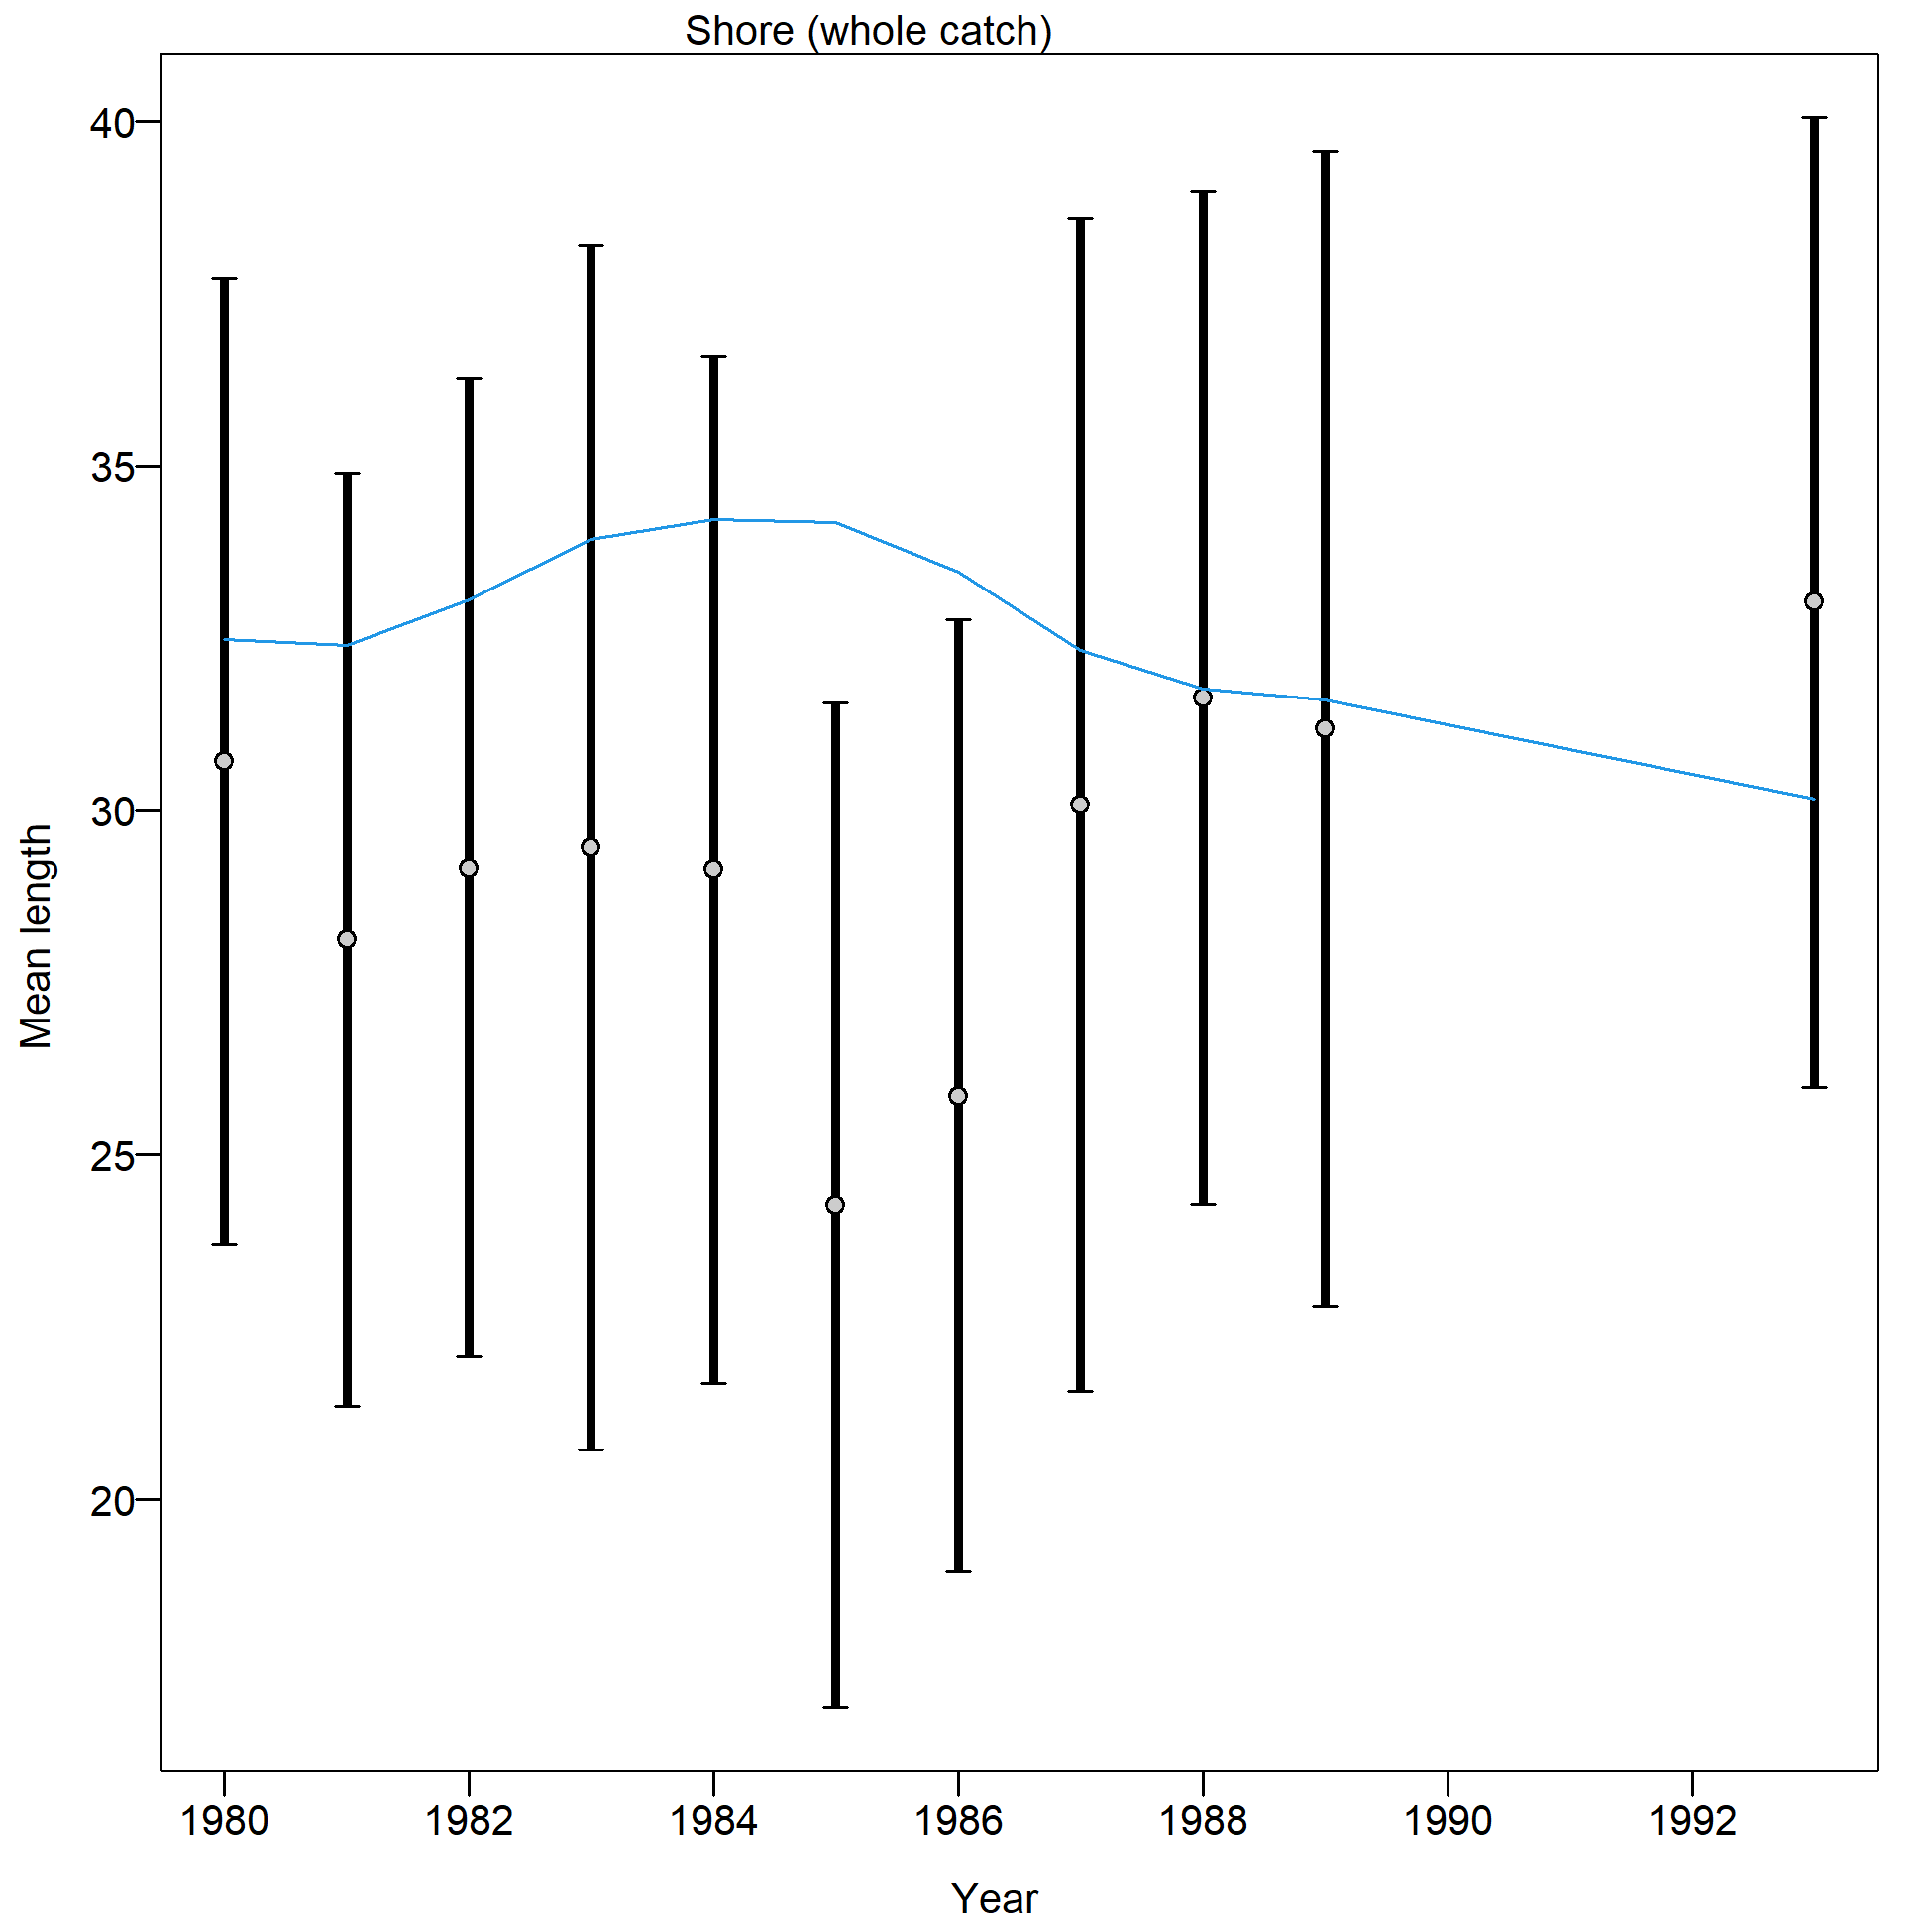
\includegraphics[width=1\textwidth,height=1\textheight]{C:/Users/Jason.Cope/Documents/Github/Sebastes_melanops_OR/Document/models/Reference model/plots/comp_lenfit_data_weighting_TA1.8_Shore.png}
\caption{Mean length (cm) index from the recreational shore-based fishery with 95 percent confidence intervals based on sample sizes and data weighting.\label{fig:shore-mean-len-fit}}
\end{figure}

\begin{figure}
\centering
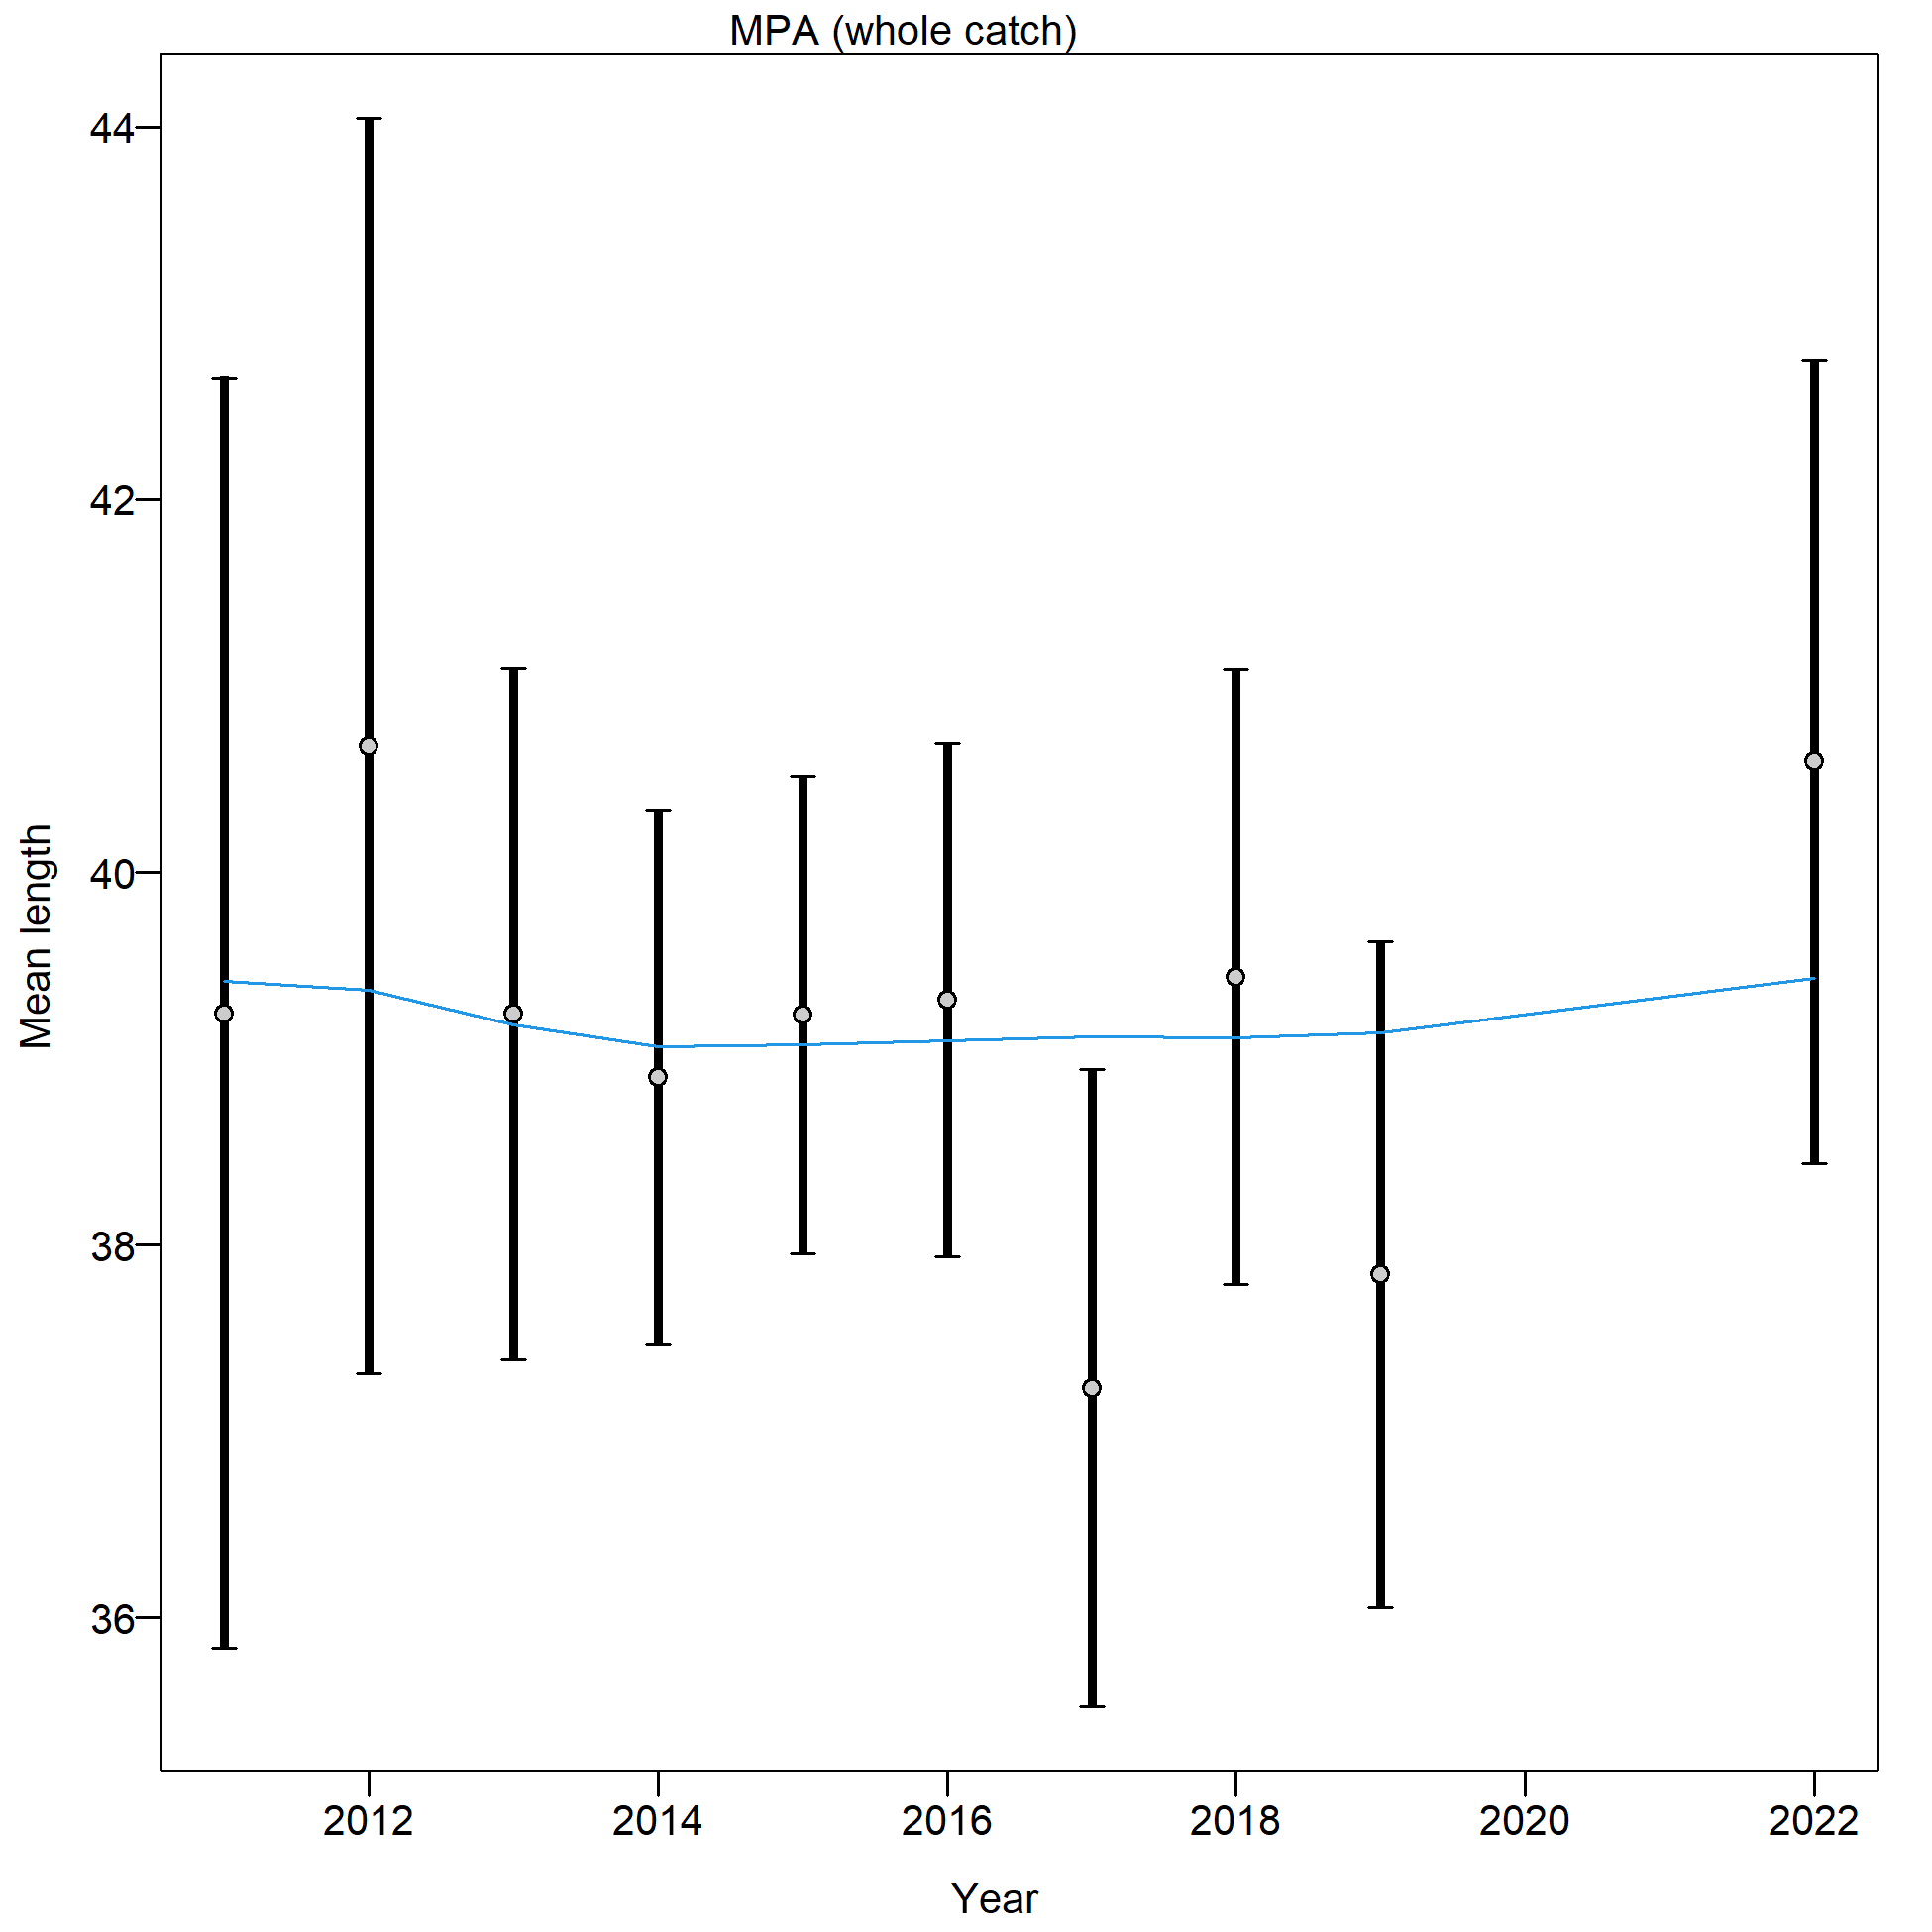
\includegraphics[width=1\textwidth,height=1\textheight]{C:/Users/Jason.Cope/Documents/Github/Sebastes_melanops_OR/Document/models/Reference model/plots/comp_lenfit_data_weighting_TA1.8_MPA.png}
\caption{Mean length (cm) index from the MPA survey with 95 percent confidence intervals based on sample sizes and data weighting.\label{fig:mpa-mean-len-fit}}
\end{figure}

\begin{figure}
\centering
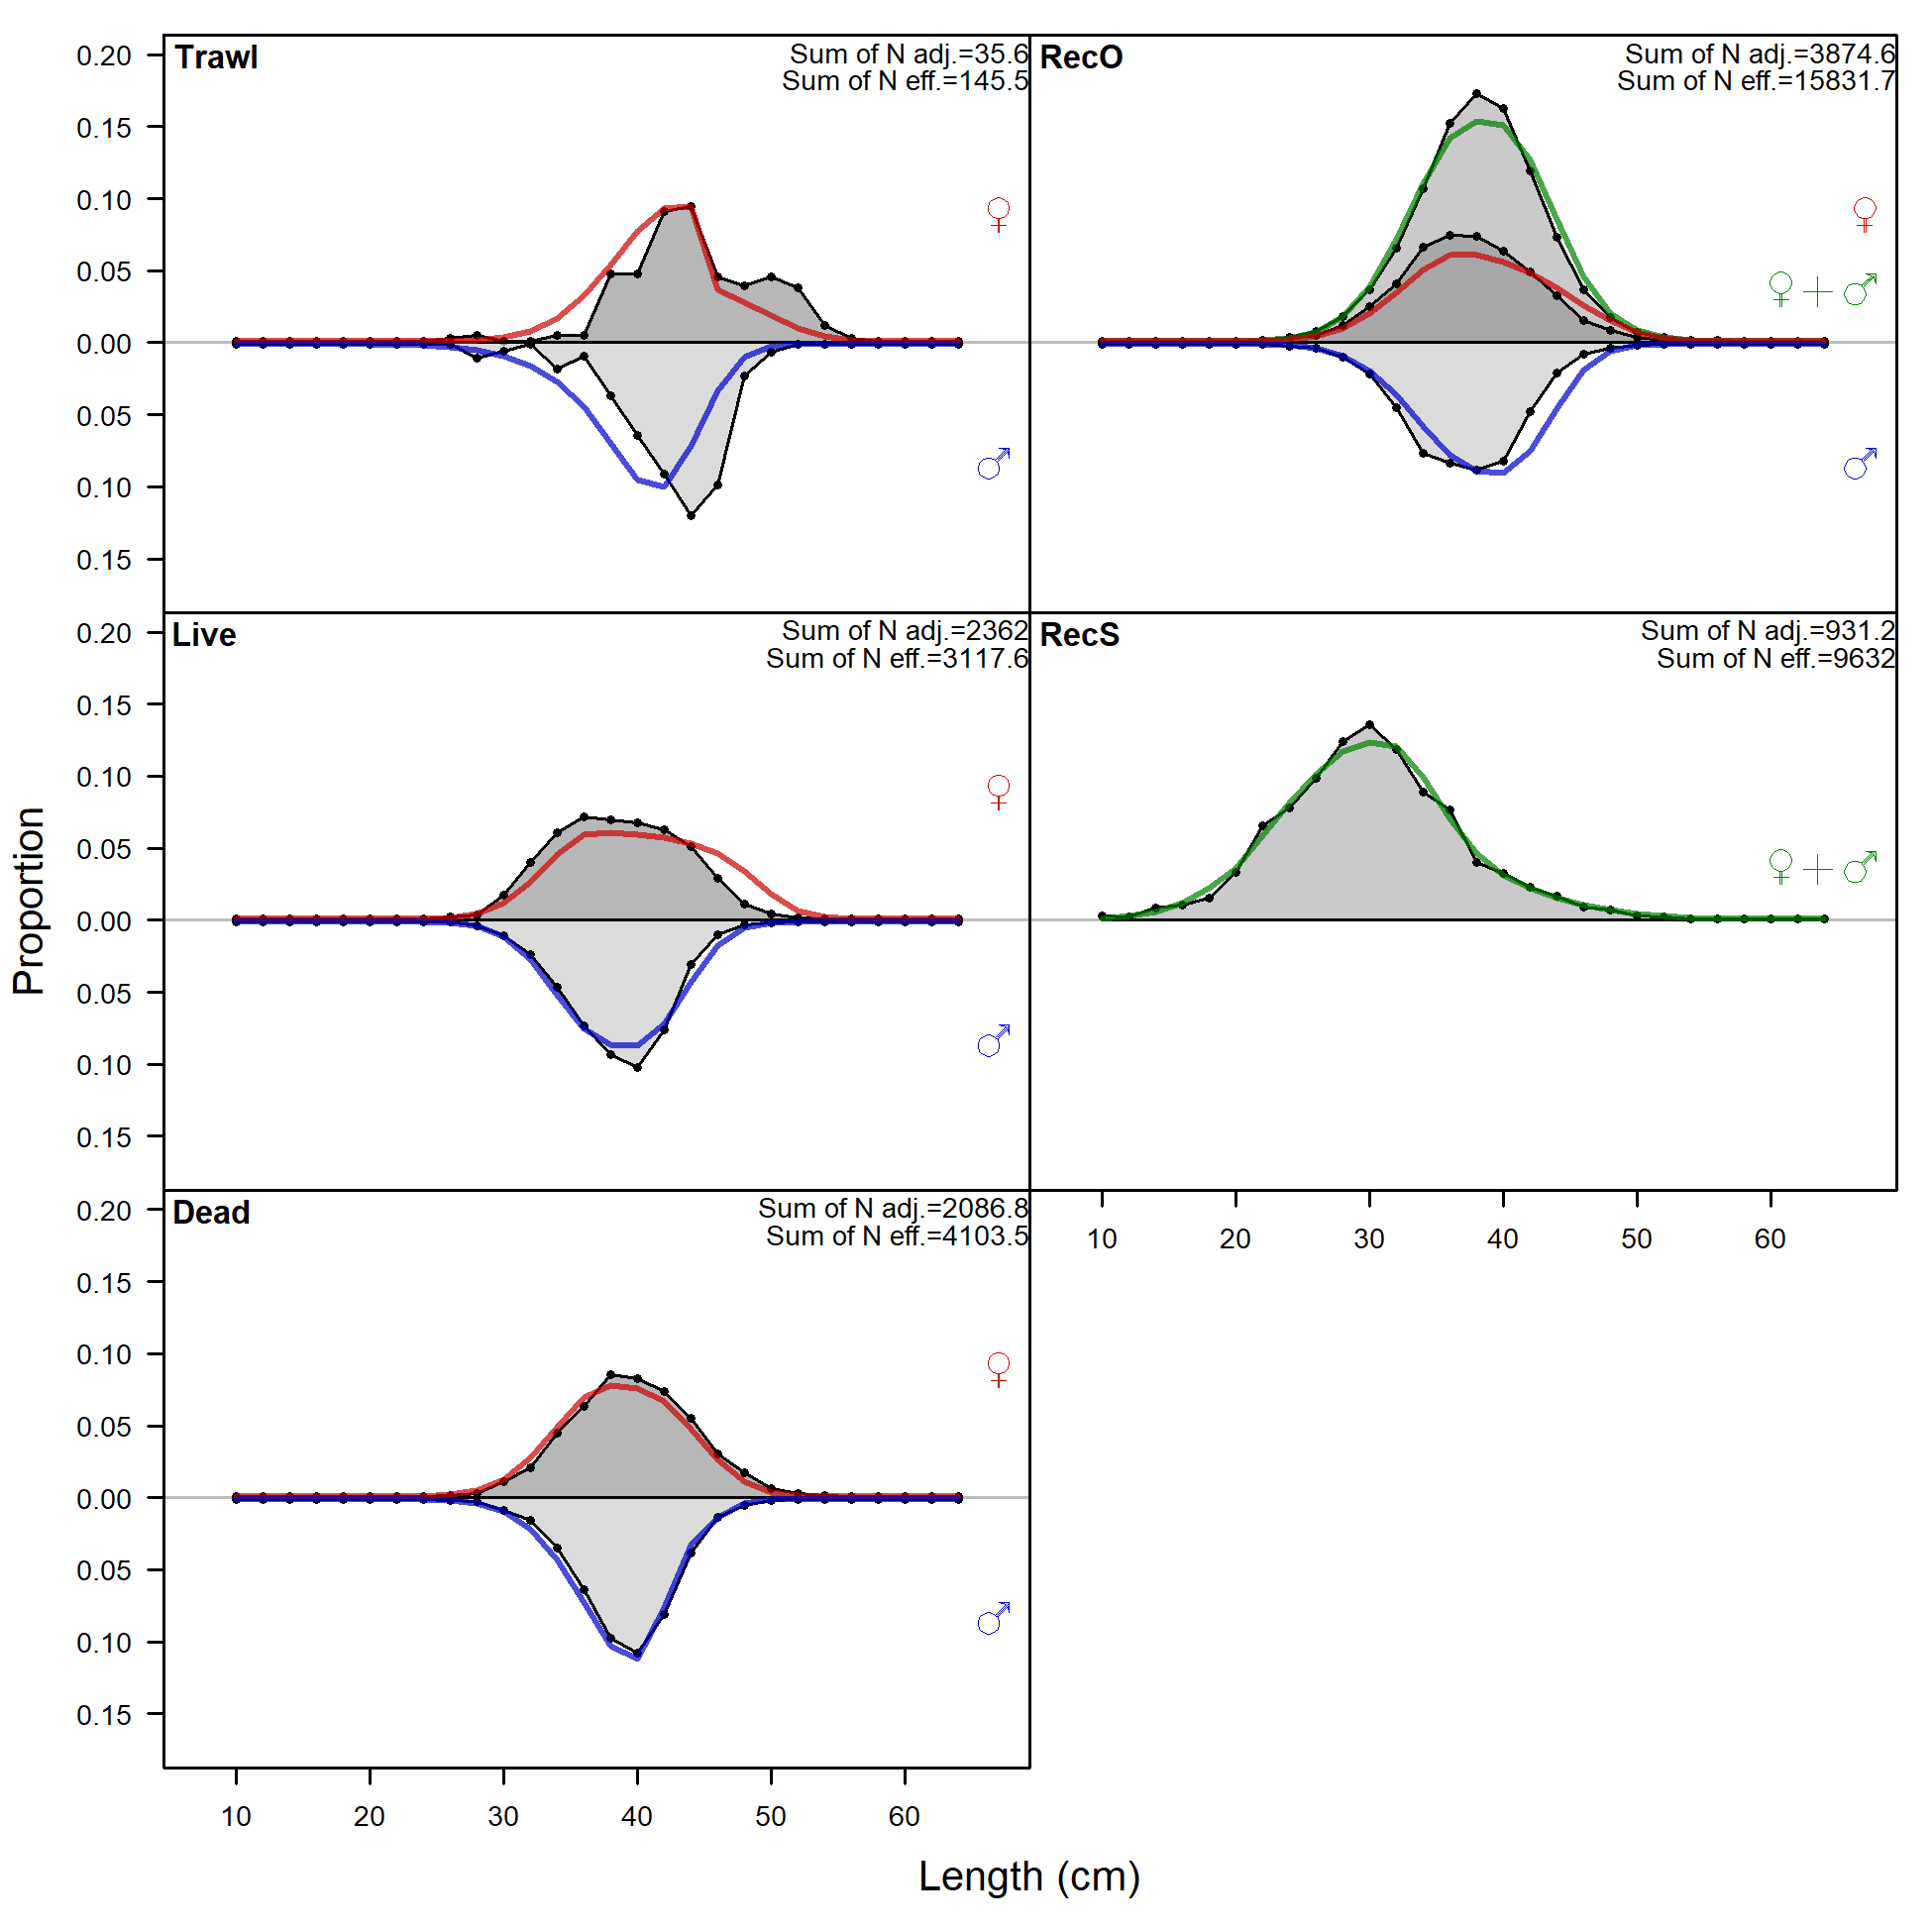
\includegraphics[width=1\textwidth,height=1\textheight]{C:/Users/Jason.Cope/Documents/Github/Sebastes_melanops_OR/Document/models/Reference model/plots/comp_lenfit__aggregated_across_time.png}
\caption{Aggregated length (cm) compositions over all years.\label{fig:agg-len-fit}}
\end{figure}

\begin{figure}
\centering
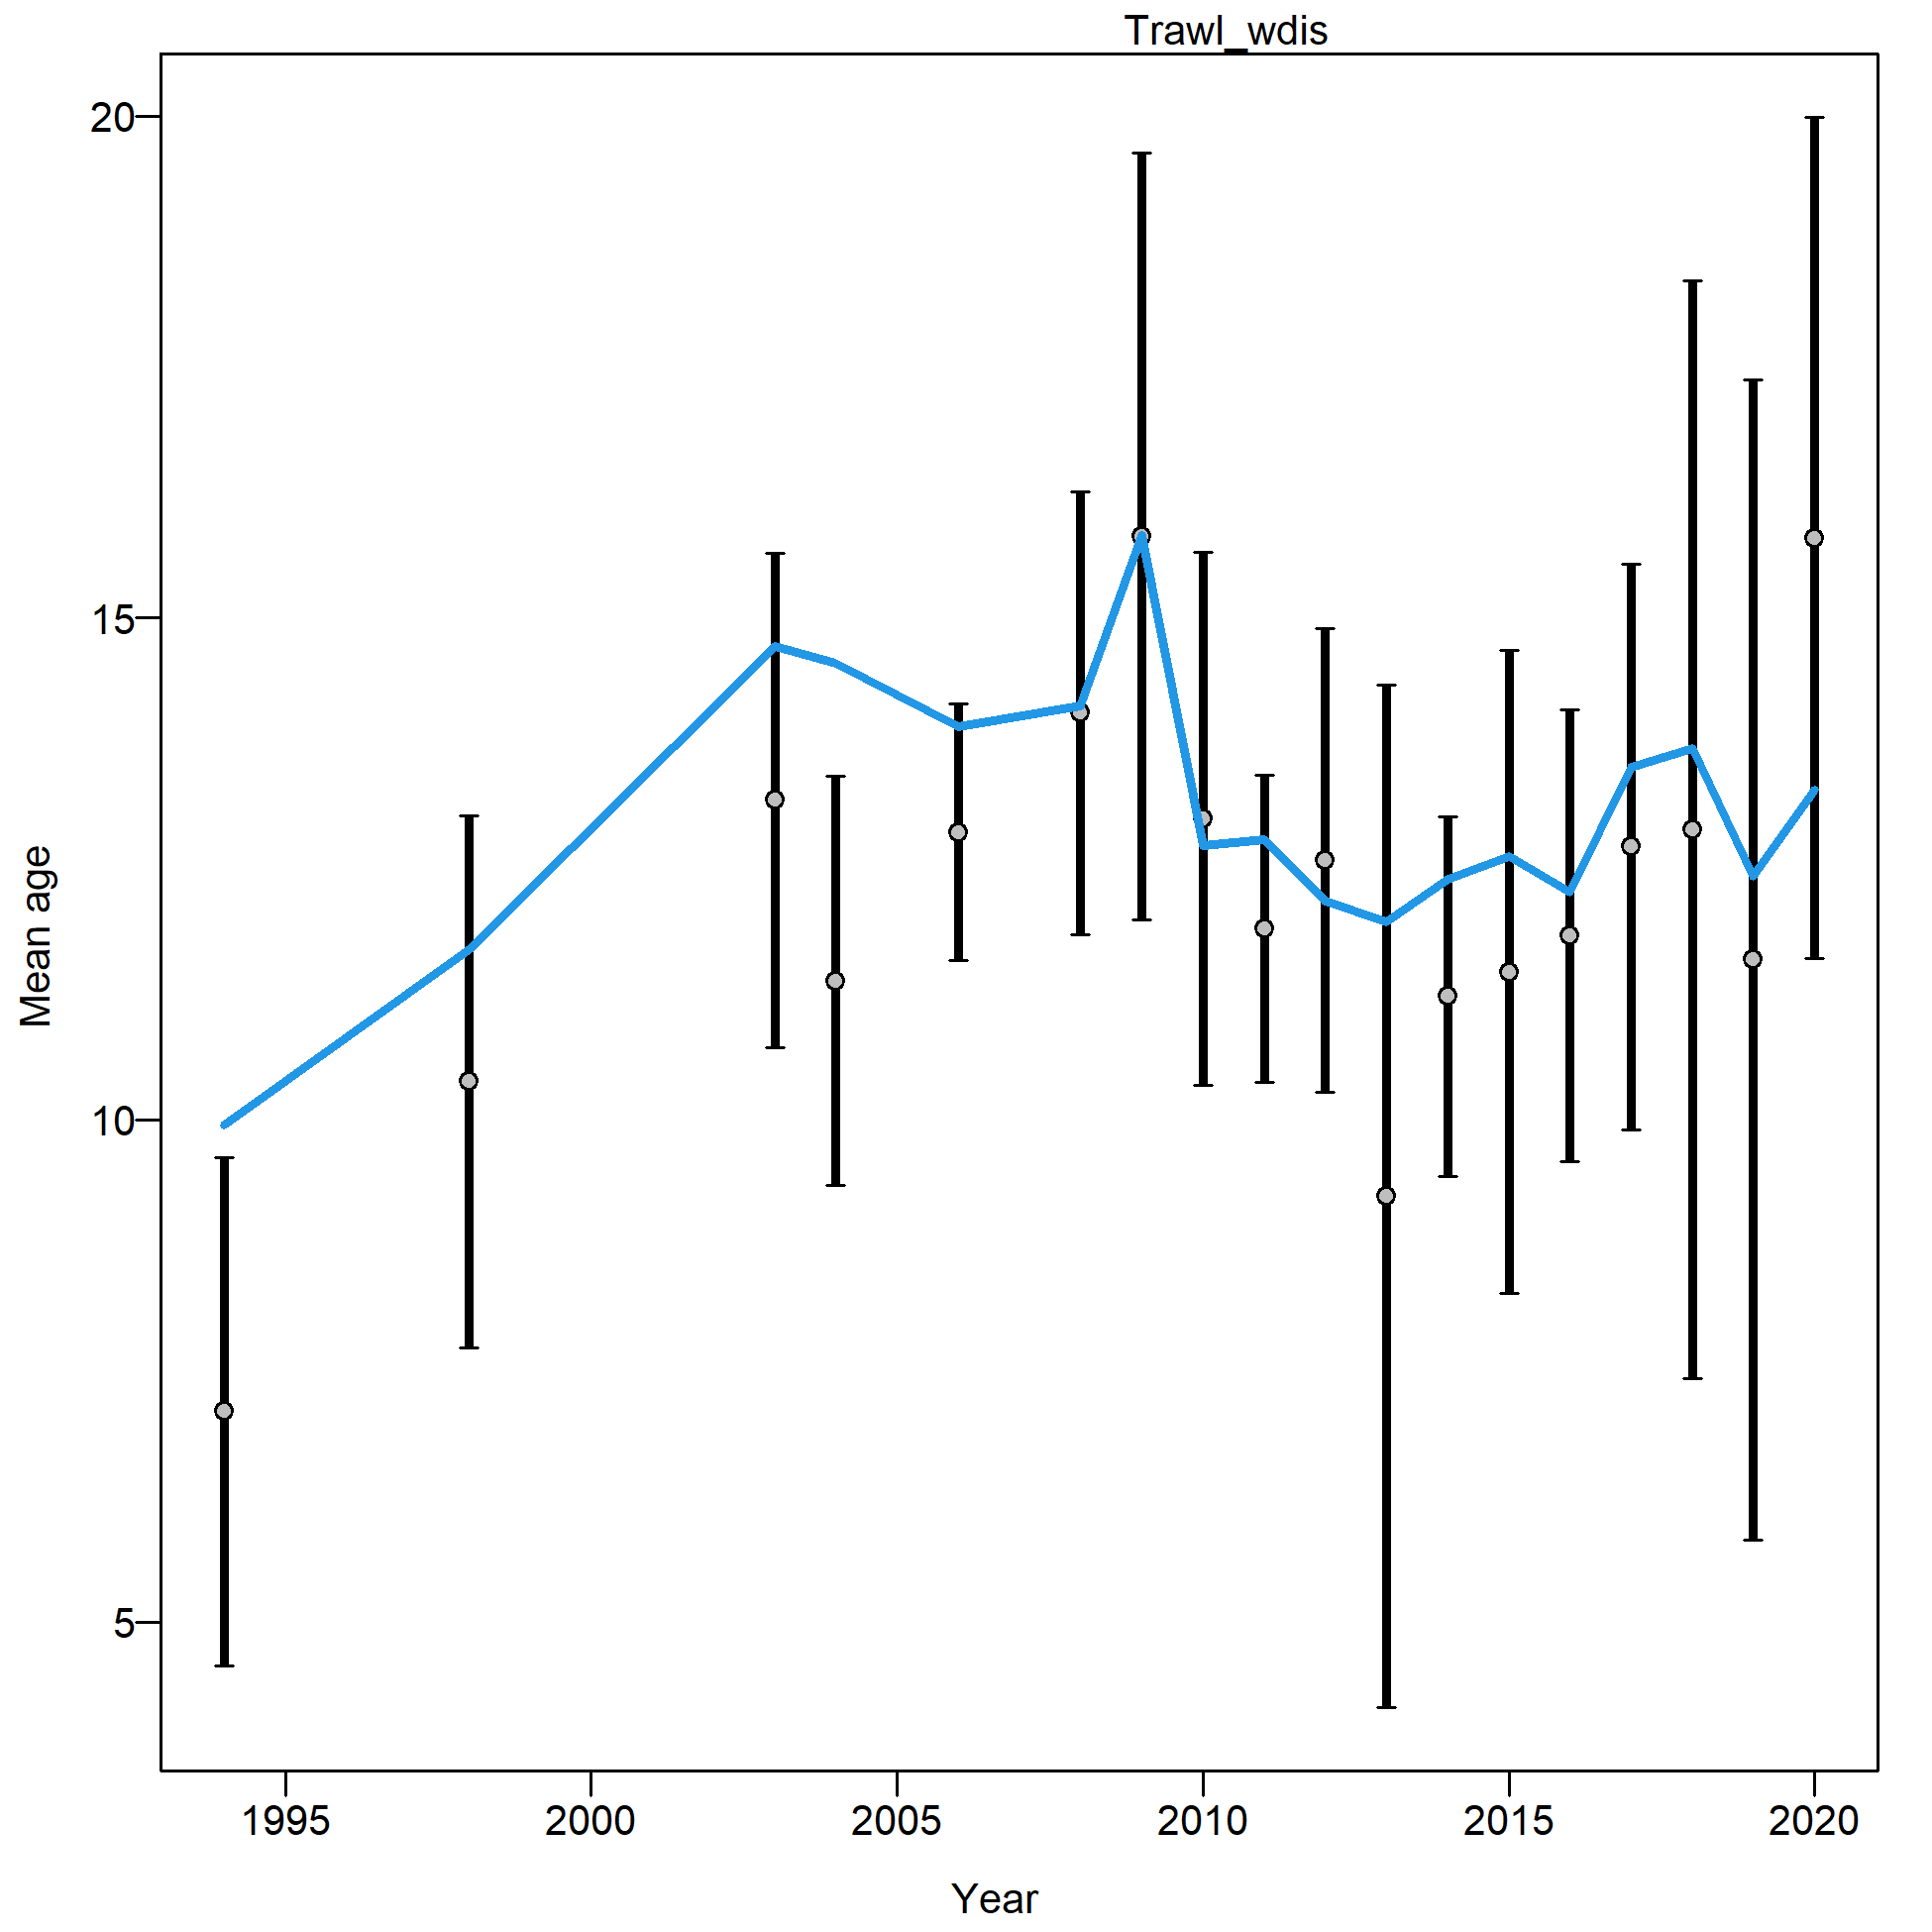
\includegraphics[width=1\textwidth,height=1\textheight]{C:/Users/Jason.Cope/Documents/Github/Sebastes_melanops_OR/Document/models/Reference model/plots/comp_condAALfit_data_weighting_TA1.8_condAgeTrawl_wdis.png}
\caption{Mean age from conditional age-at-length data for the commercial trawl fishery.\label{fig:trawl-mean-caal}}
\end{figure}

\begin{figure}
\centering
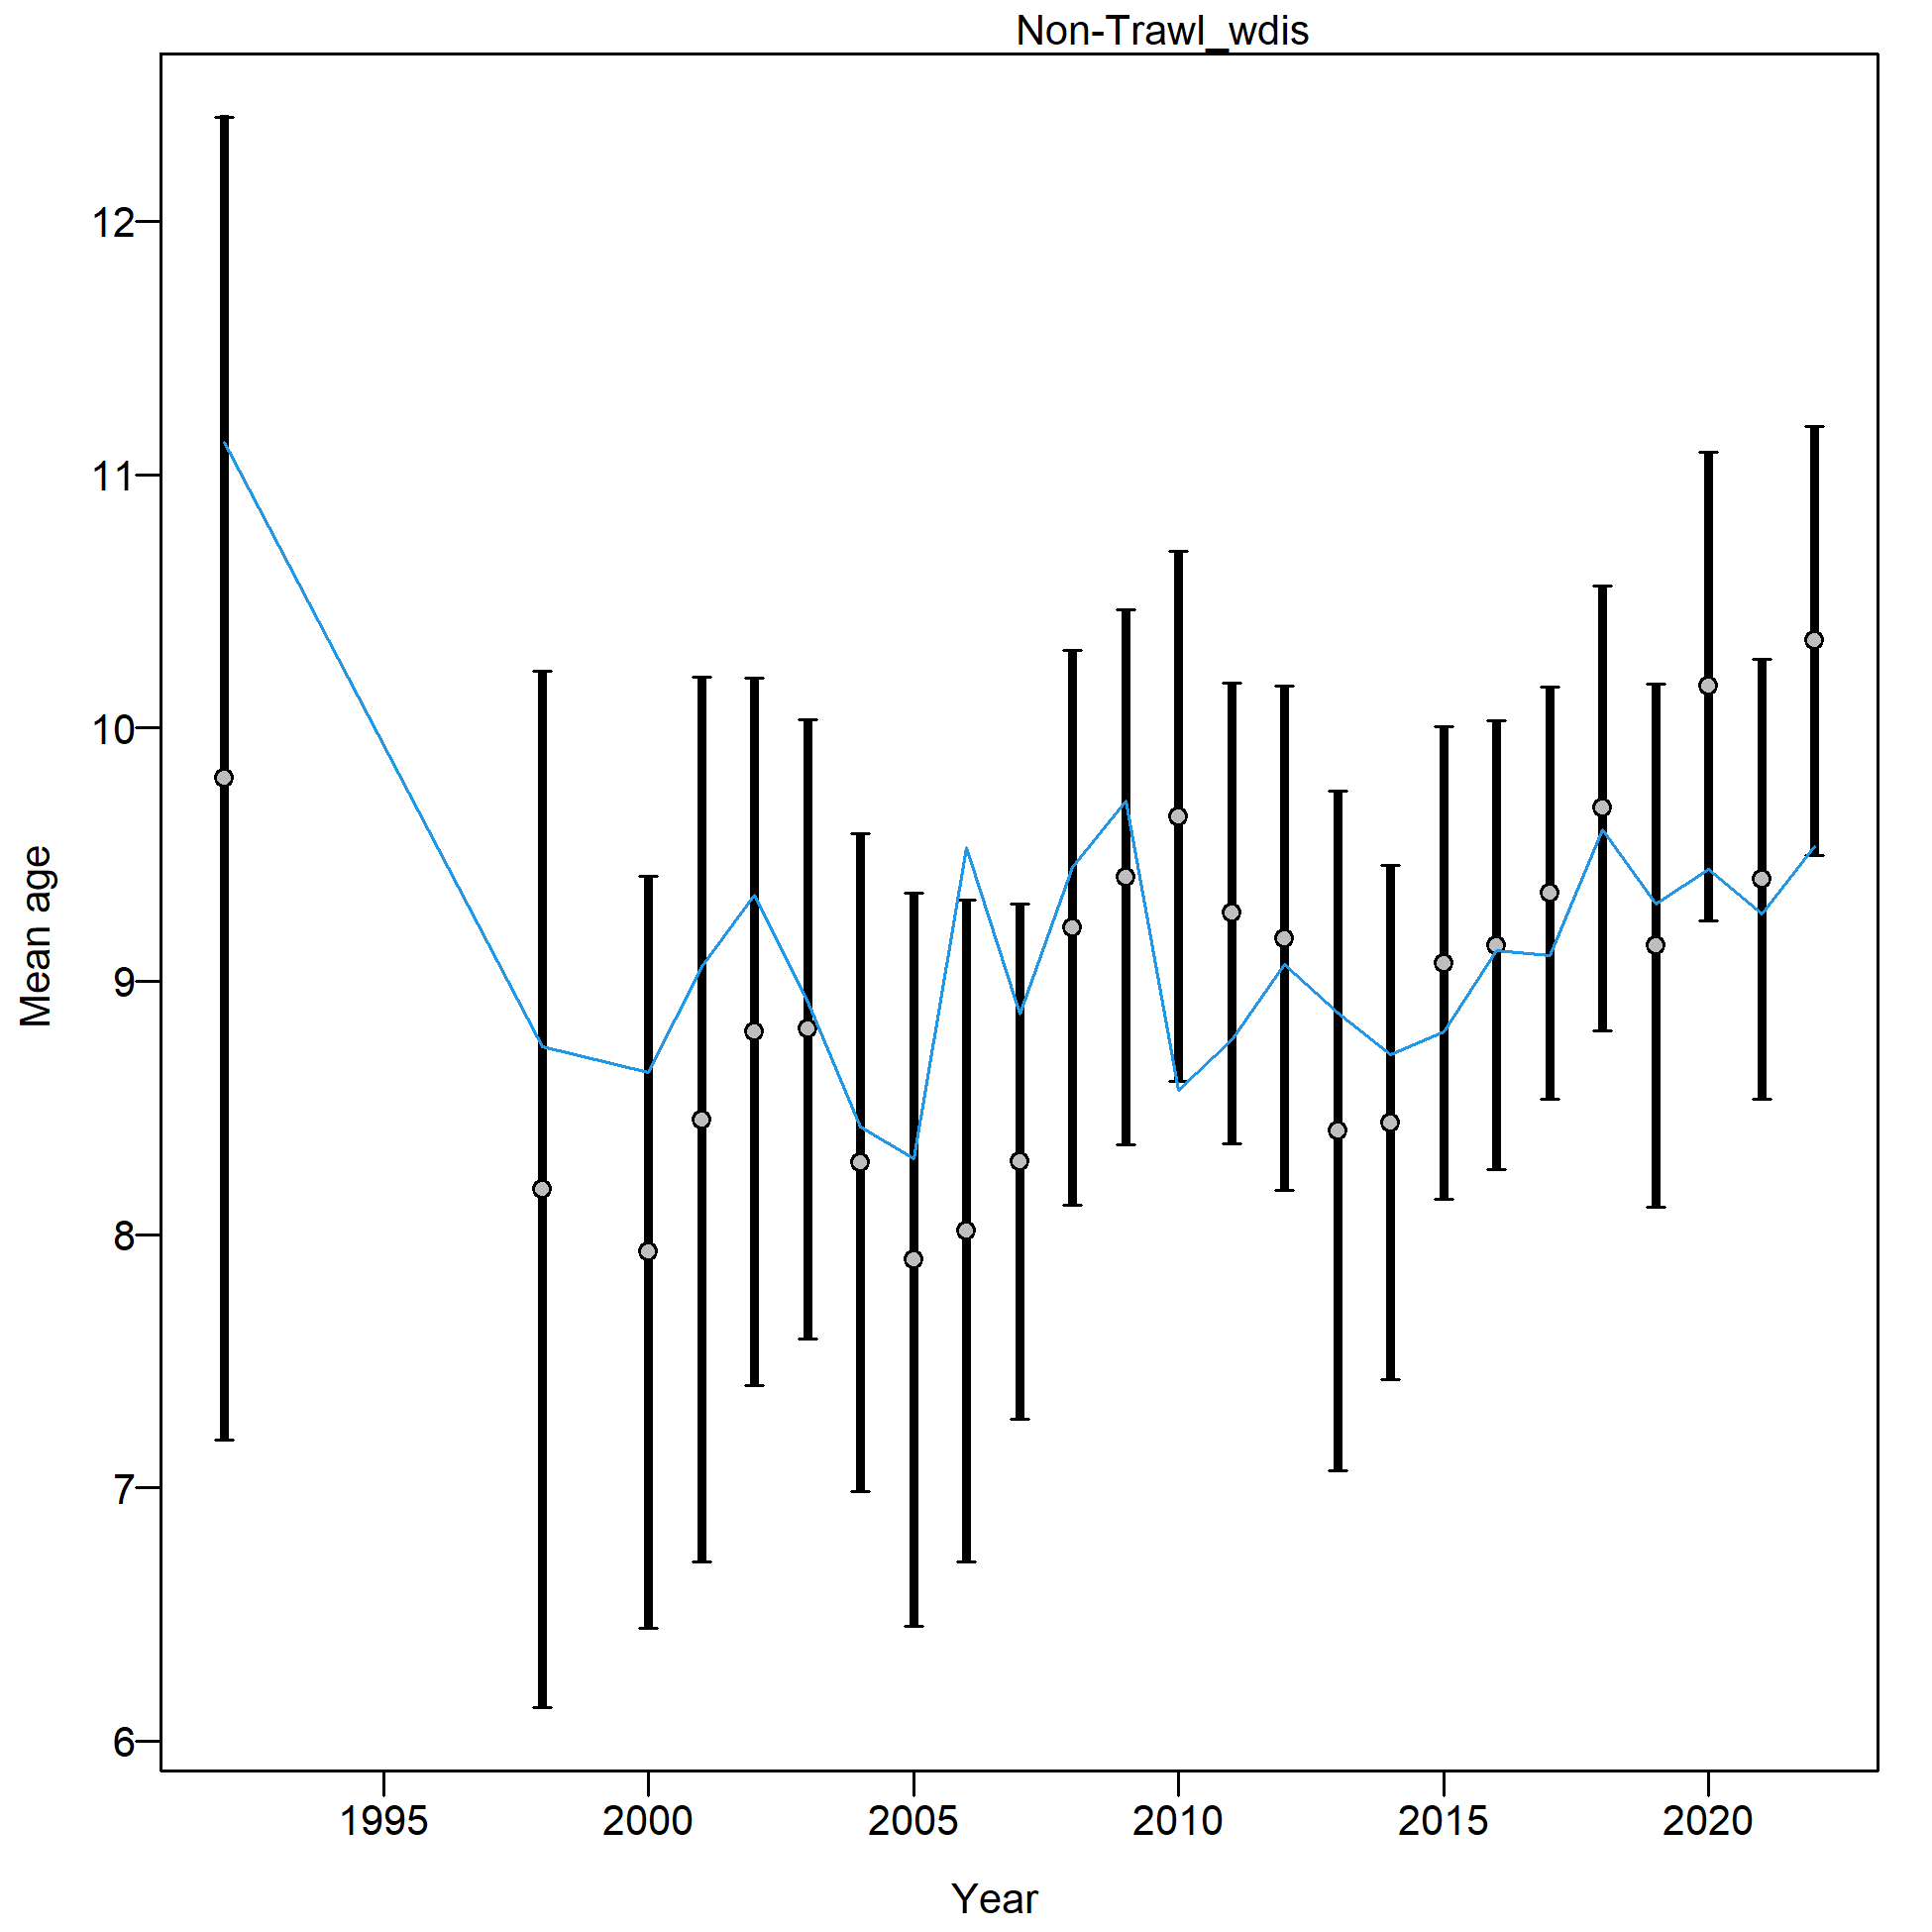
\includegraphics[width=1\textwidth,height=1\textheight]{C:/Users/Jason.Cope/Documents/Github/Sebastes_melanops_OR/Document/models/Reference model/plots/comp_condAALfit_data_weighting_TA1.8_condAgeNon-Trawl_wdis.png}
\caption{Mean age observations from the conditional age-at-length data from the non-trawl commercial fishery.\label{fig:nontrawl-mean-caal}}
\end{figure}

\begin{figure}
\centering
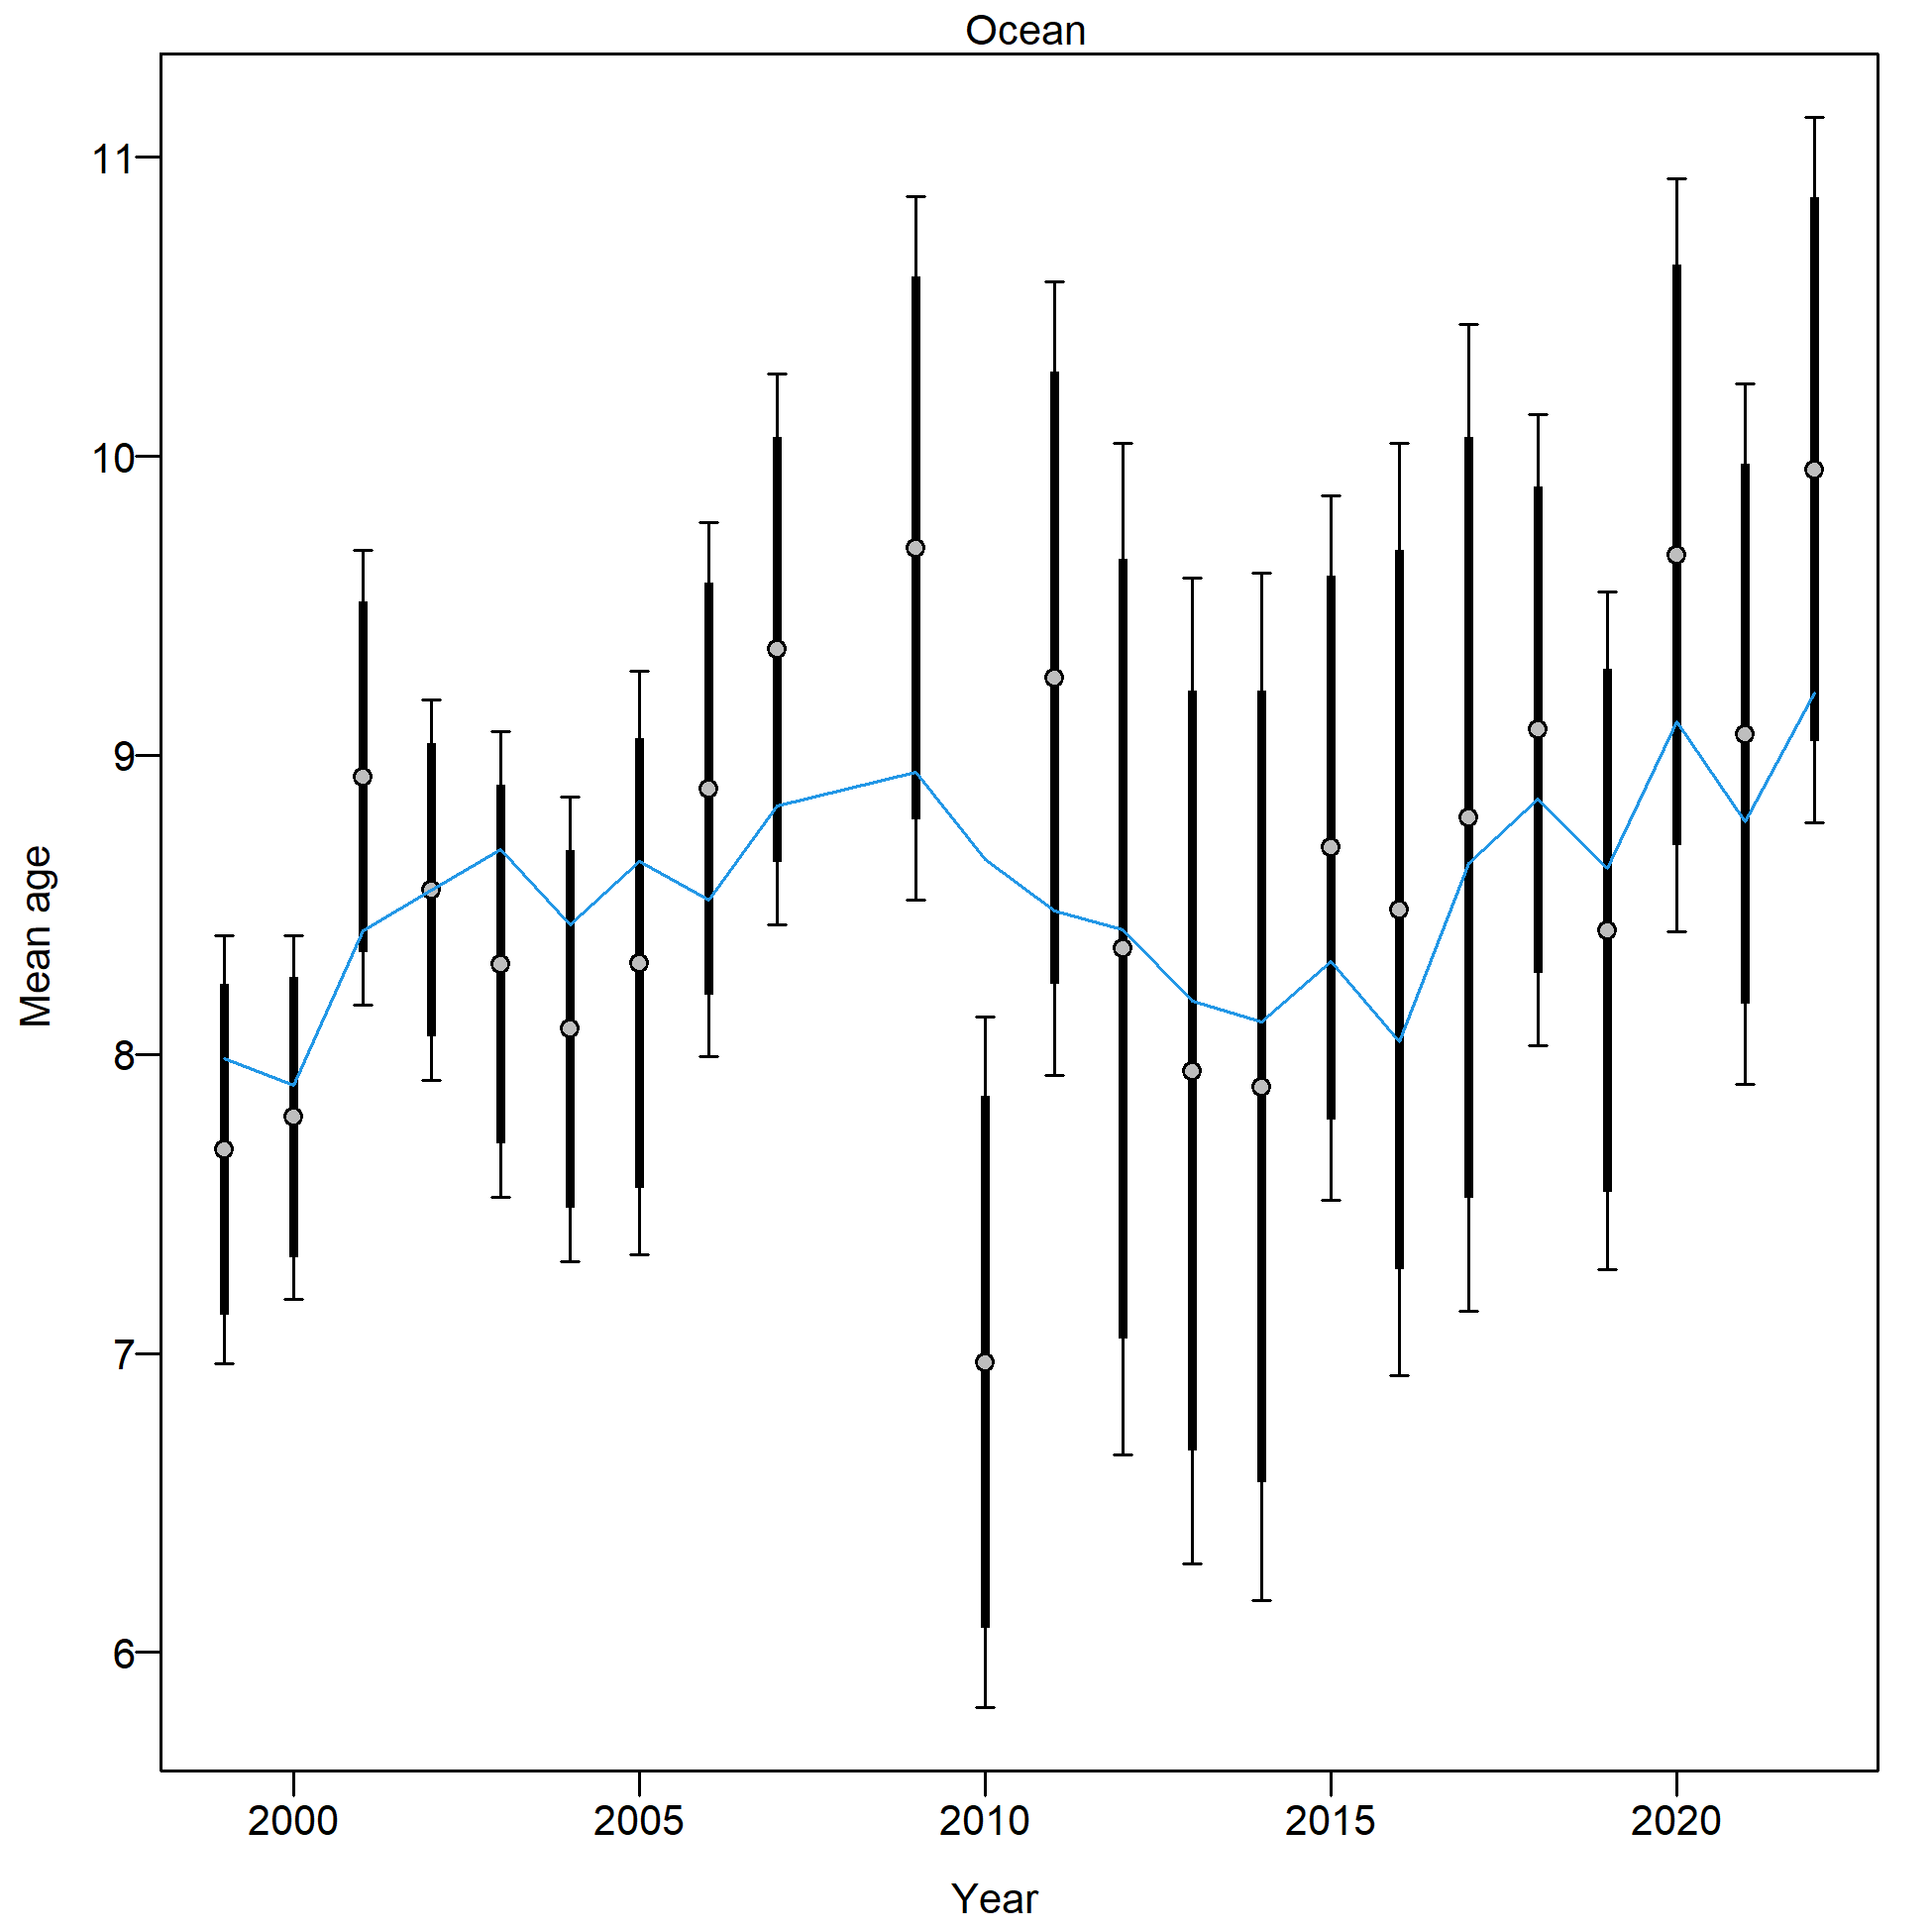
\includegraphics[width=1\textwidth,height=1\textheight]{C:/Users/Jason.Cope/Documents/Github/Sebastes_melanops_OR/Document/models/Reference model/plots/comp_condAALfit_data_weighting_TA1.8_condAgeOcean.png}
\caption{Mean age observations from the conditional age-at-length data from the ocean boat fishery.\label{fig:ocean-mean-caal}}
\end{figure}

\begin{figure}
\centering
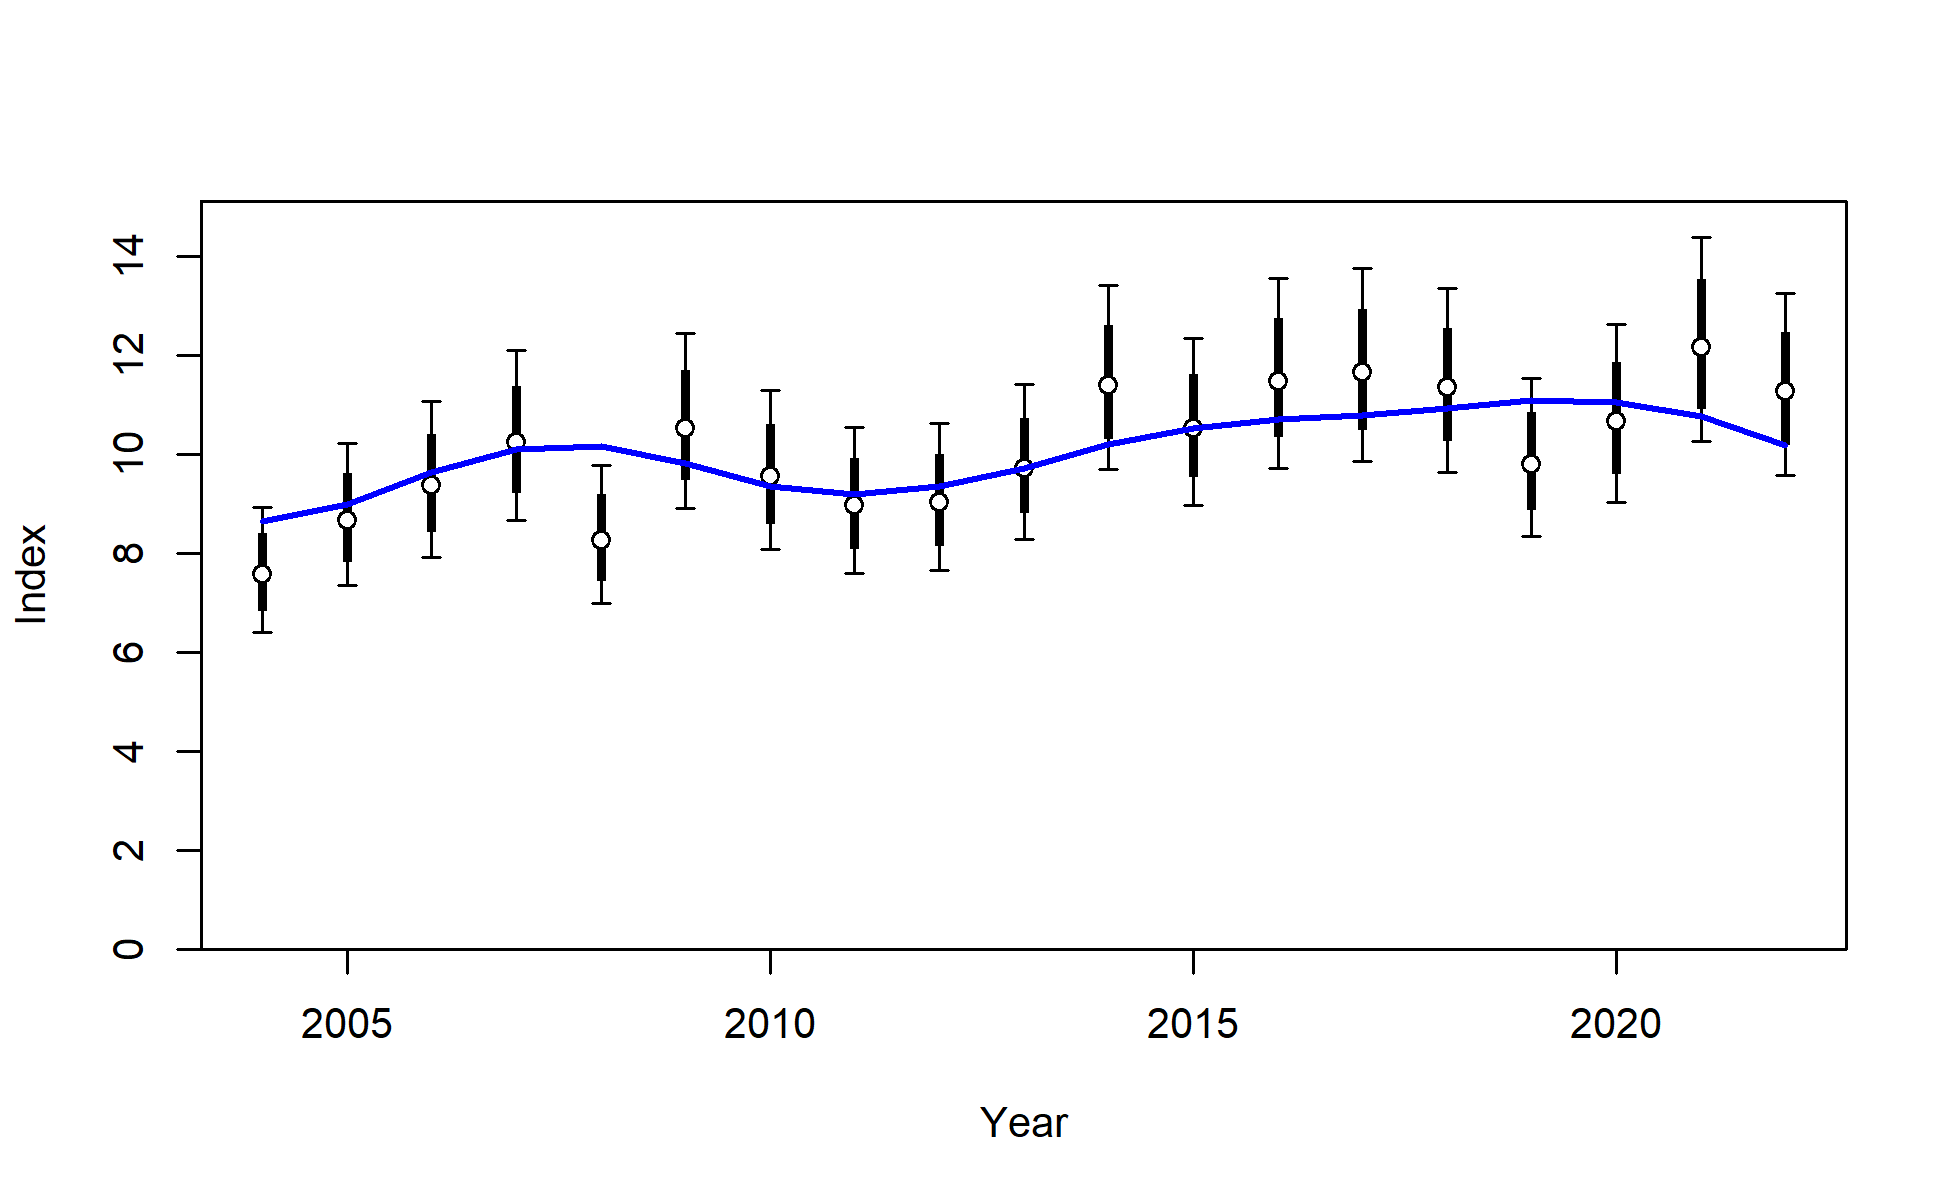
\includegraphics[width=1\textwidth,height=1\textheight]{C:/Users/Jason.Cope/Documents/Github/Sebastes_melanops_OR/Document/models/Reference model/plots/index2_cpuefit_Non-Trawl_wdis.png}
\caption{Fit to the non-trawl commercial survey index of abundance.\label{fig:nontrawl-index-fit}}
\end{figure}

\begin{figure}
\centering
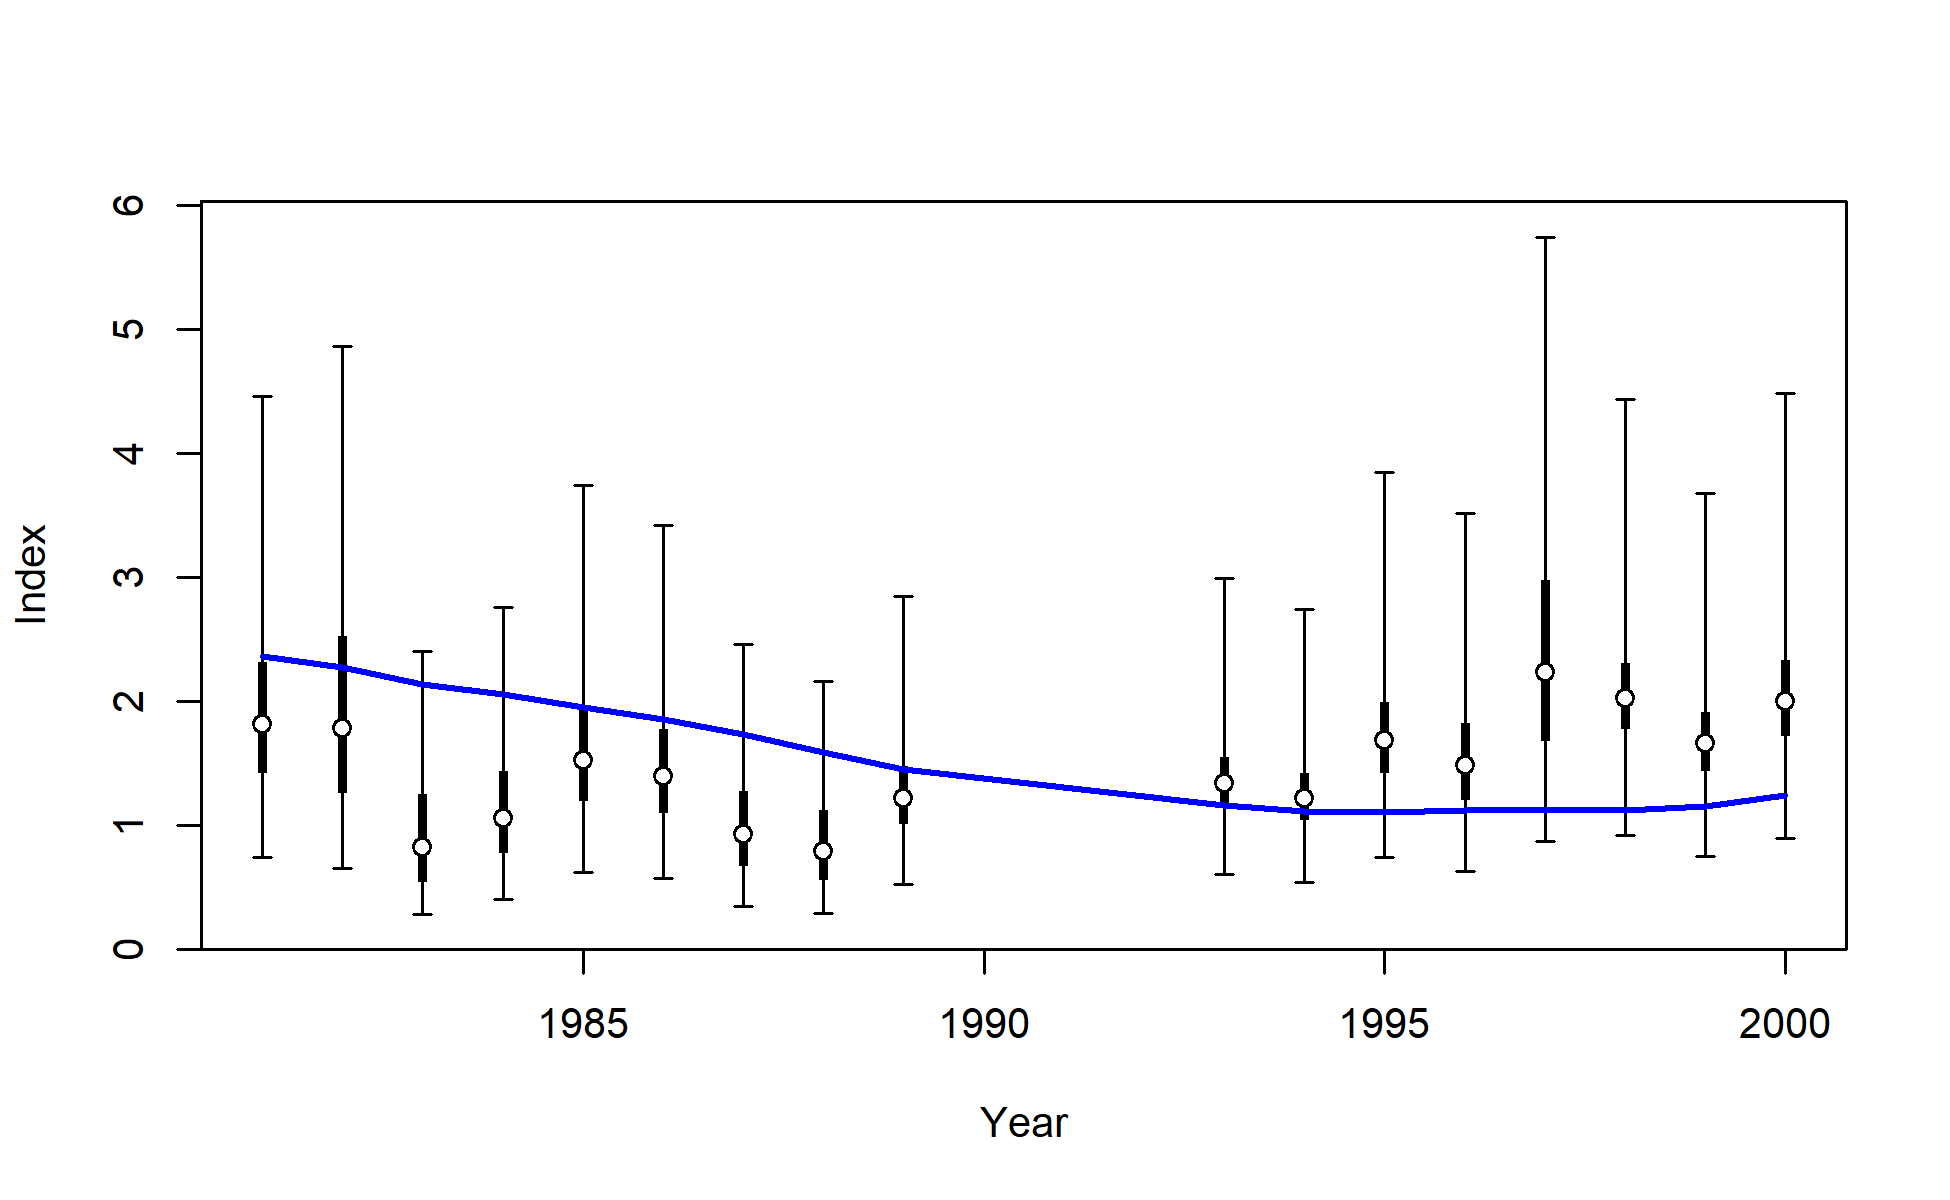
\includegraphics[width=1\textwidth,height=1\textheight]{C:/Users/Jason.Cope/Documents/Github/Sebastes_melanops_OR/Document/models/Reference model/plots/index2_cpuefit_MRFSS.png}
\caption{Fit to the MRFSS recreational survey index of abundance.\label{fig:mrfss-index-fit}}
\end{figure}

\begin{figure}
\centering
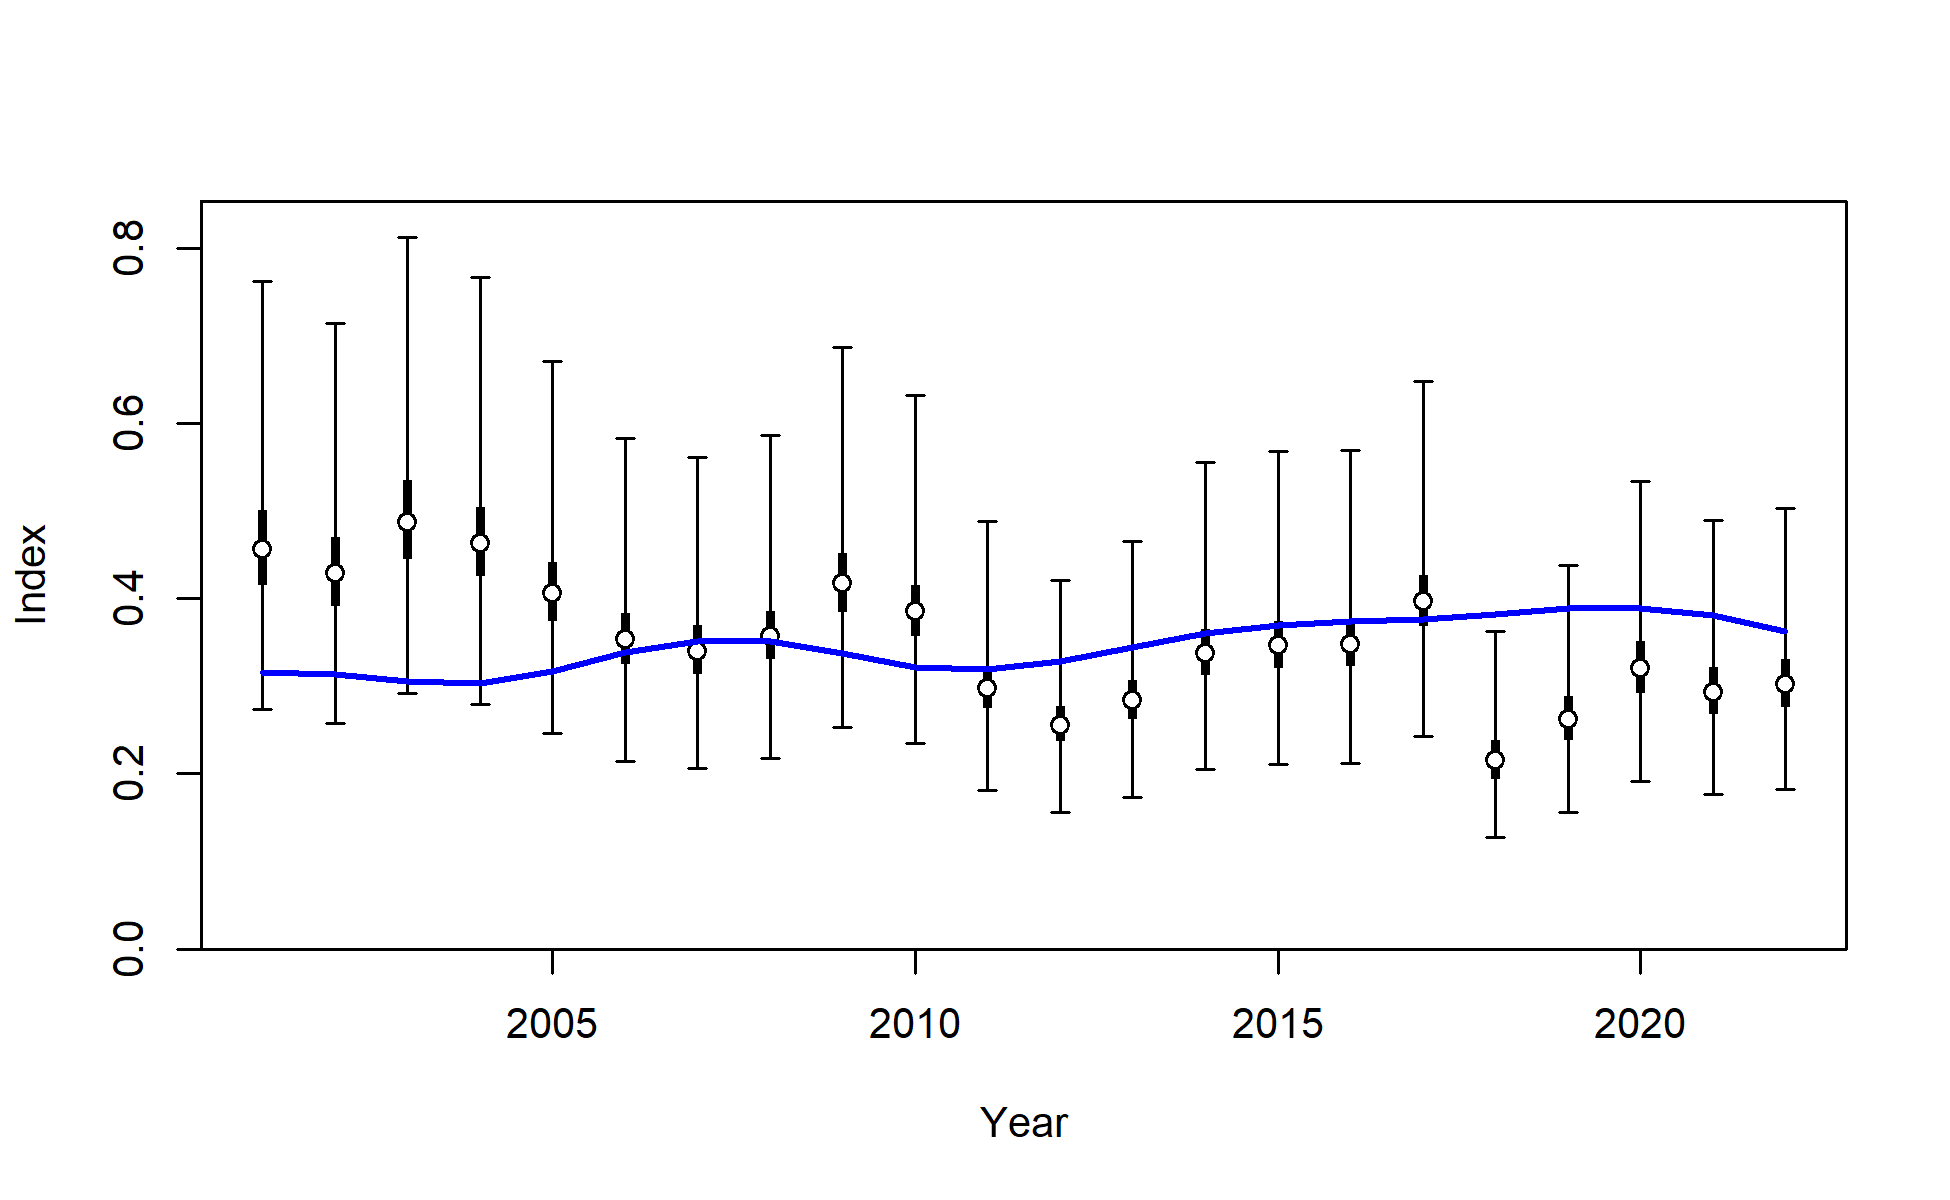
\includegraphics[width=1\textwidth,height=1\textheight]{C:/Users/Jason.Cope/Documents/Github/Sebastes_melanops_OR/Document/models/Reference model/plots/index2_cpuefit_Ocean.png}
\caption{Fit to the MRFSS recreational survey index of abundance.\label{fig:orbs-index-fit}}
\end{figure}

\begin{figure}
\centering
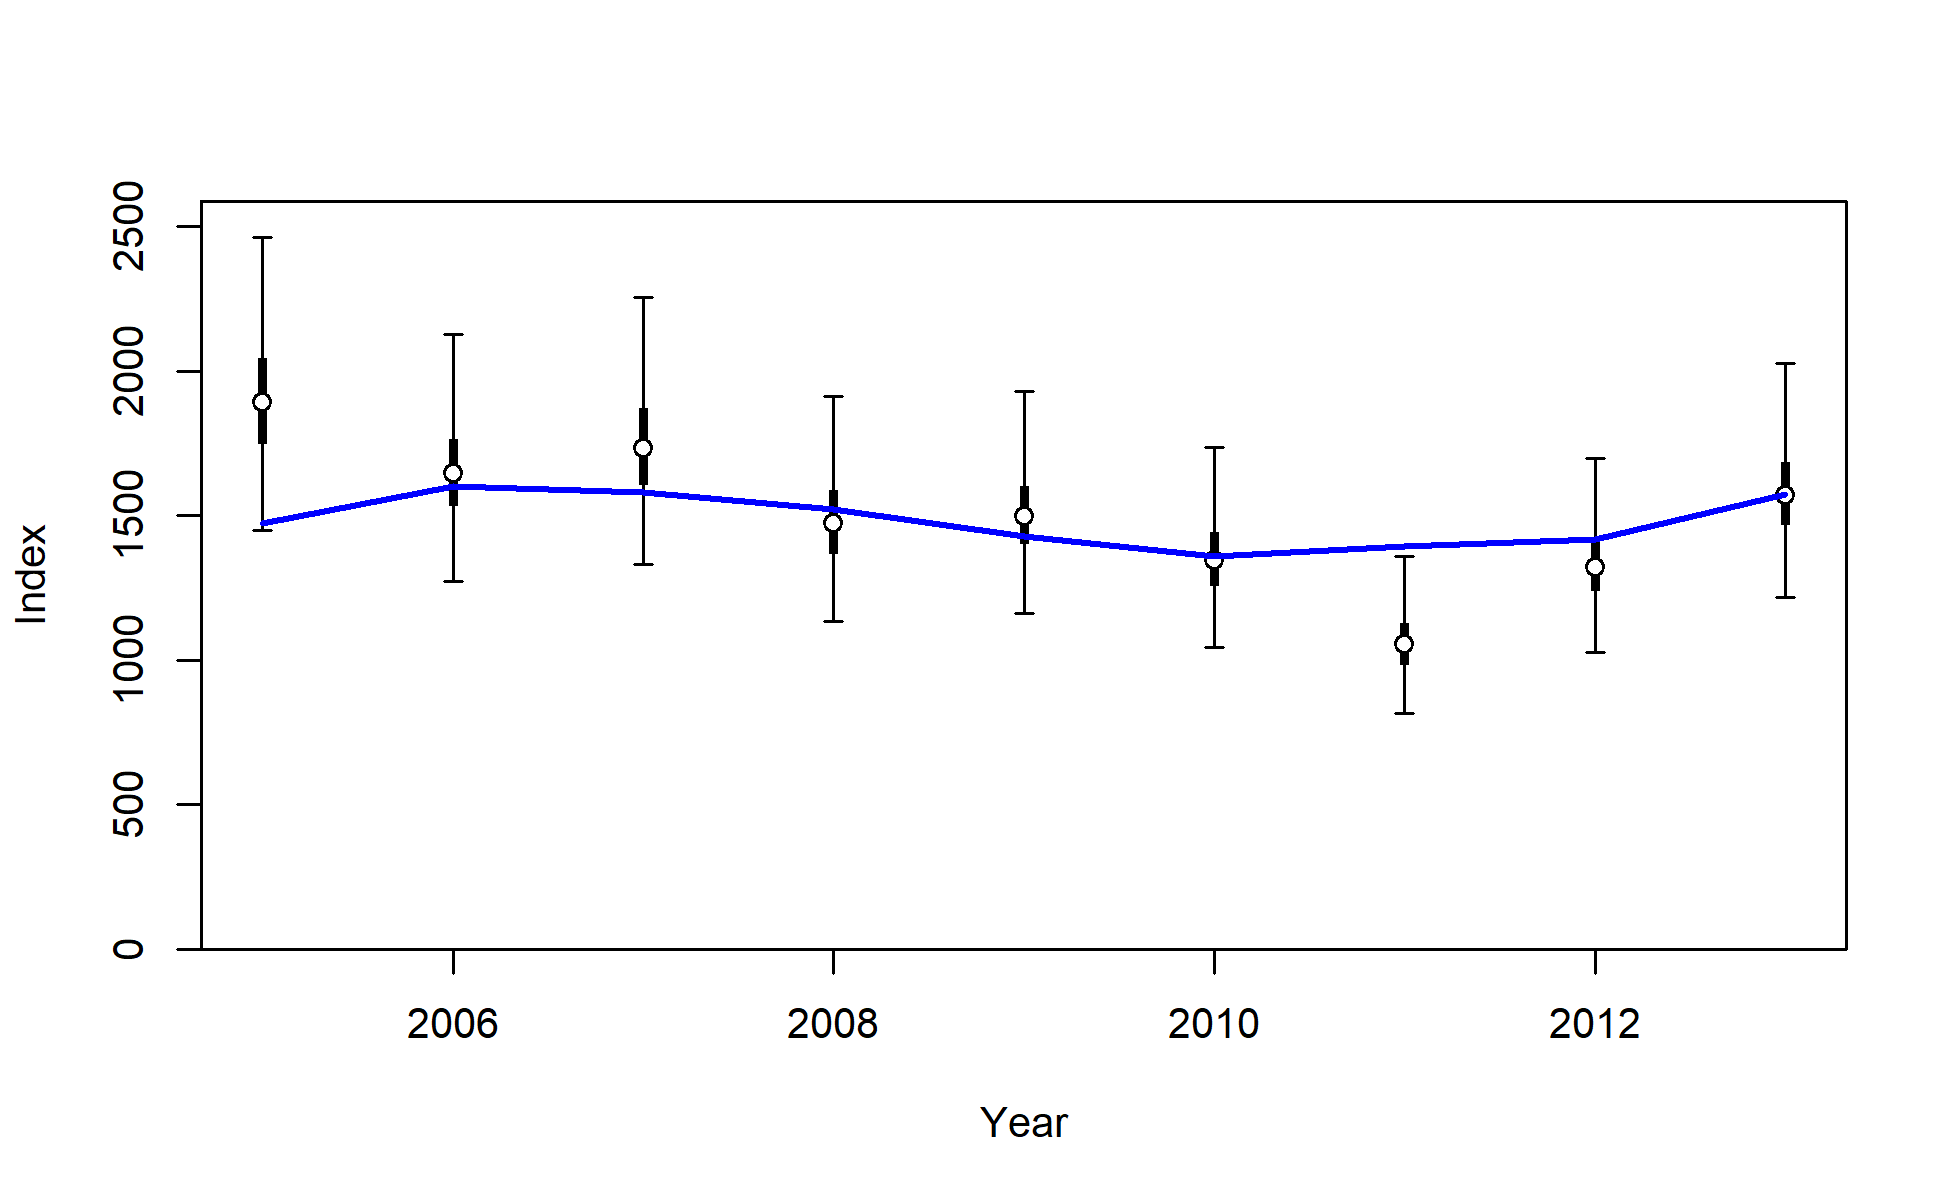
\includegraphics[width=1\textwidth,height=1\textheight]{C:/Users/Jason.Cope/Documents/Github/Sebastes_melanops_OR/Document/models/Reference model/plots/index2_cpuefit_Tag.png}
\caption{Fit to the tagging survey index of abundance.\label{fig:tag-index-fit}}
\end{figure}

\begin{figure}
\centering
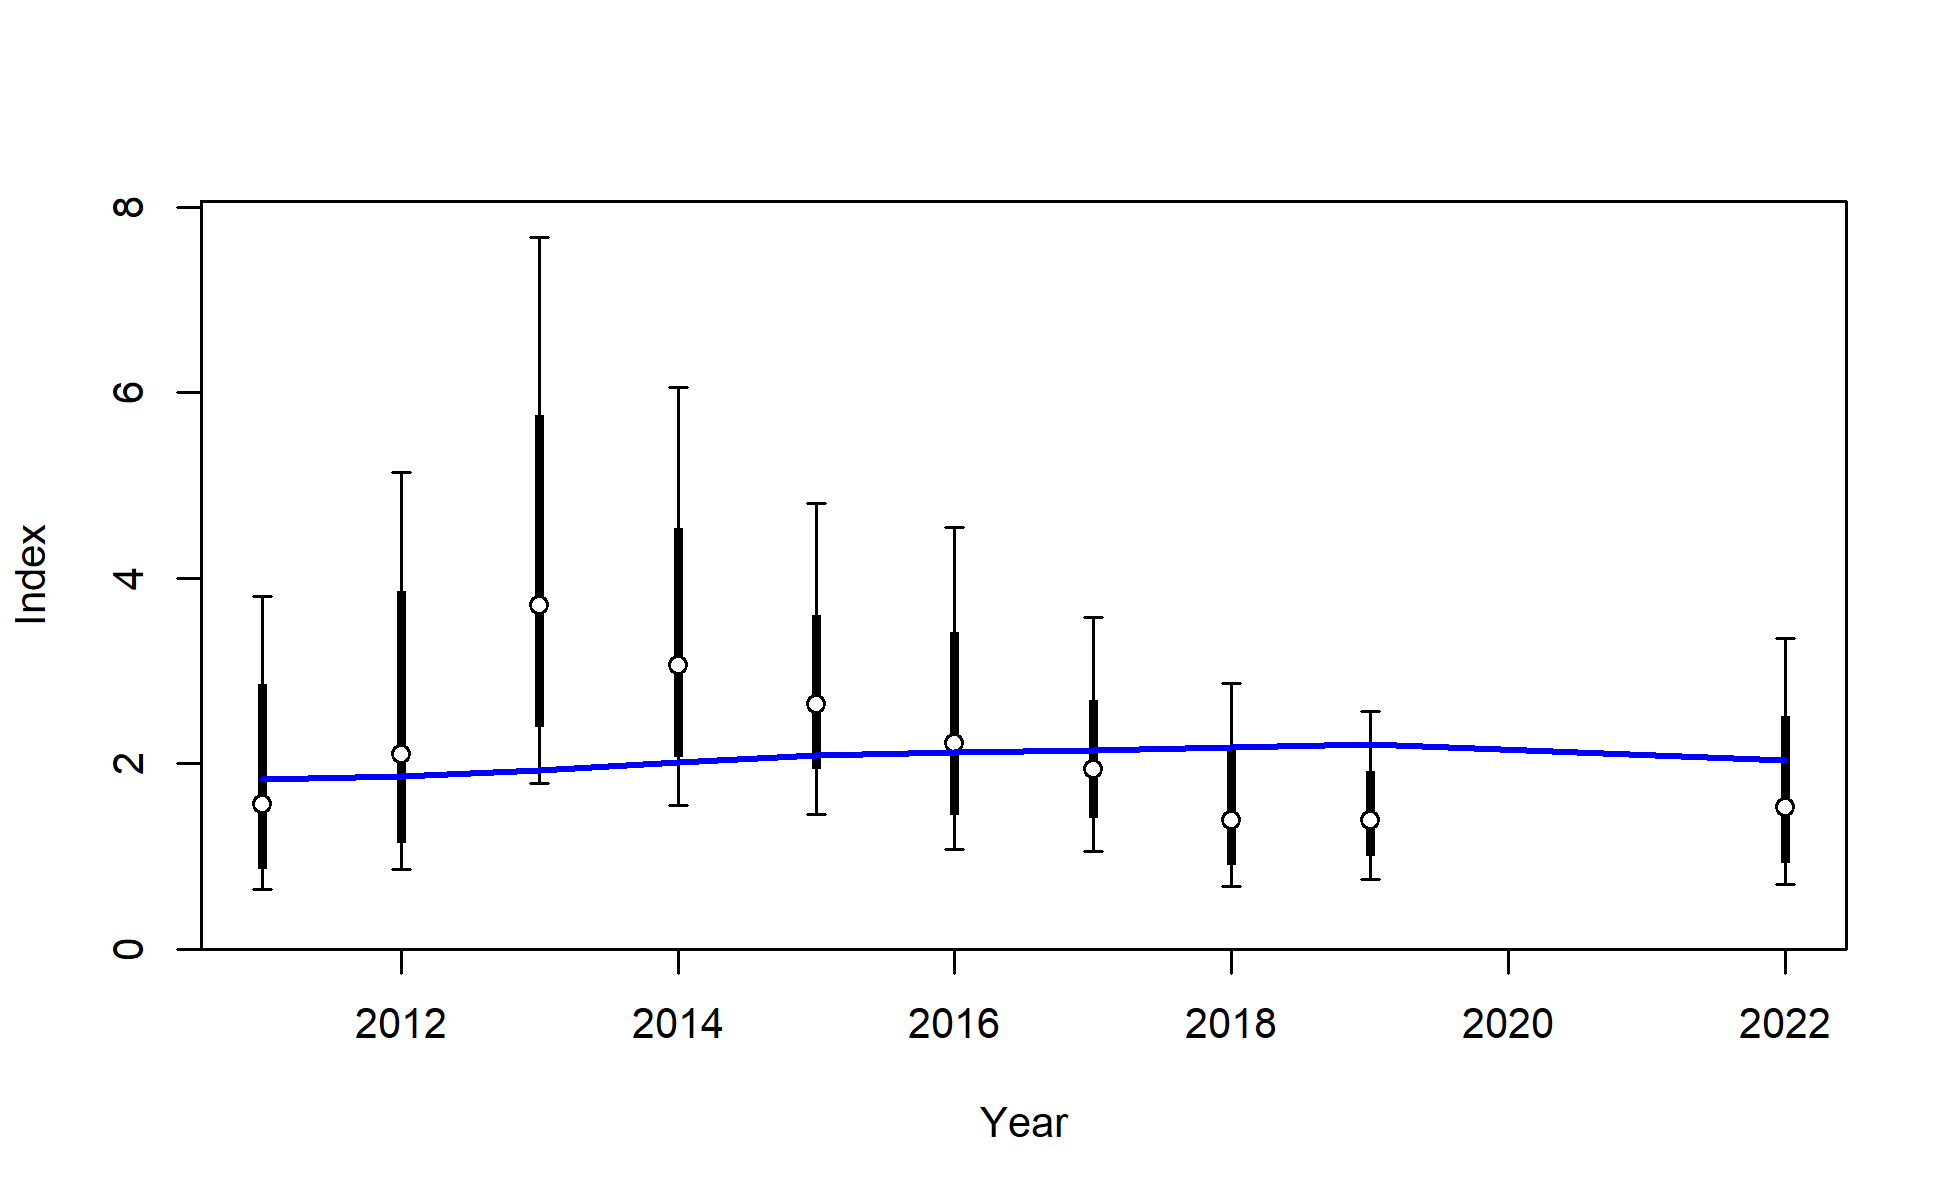
\includegraphics[width=1\textwidth,height=1\textheight]{C:/Users/Jason.Cope/Documents/Github/Sebastes_melanops_OR/Document/models/Reference model/plots/index2_cpuefit_MPA.png}
\caption{Fit to the MPA survey index of abundance.\label{fig:mpa-index-fit}}
\end{figure}

\begin{figure}
\centering
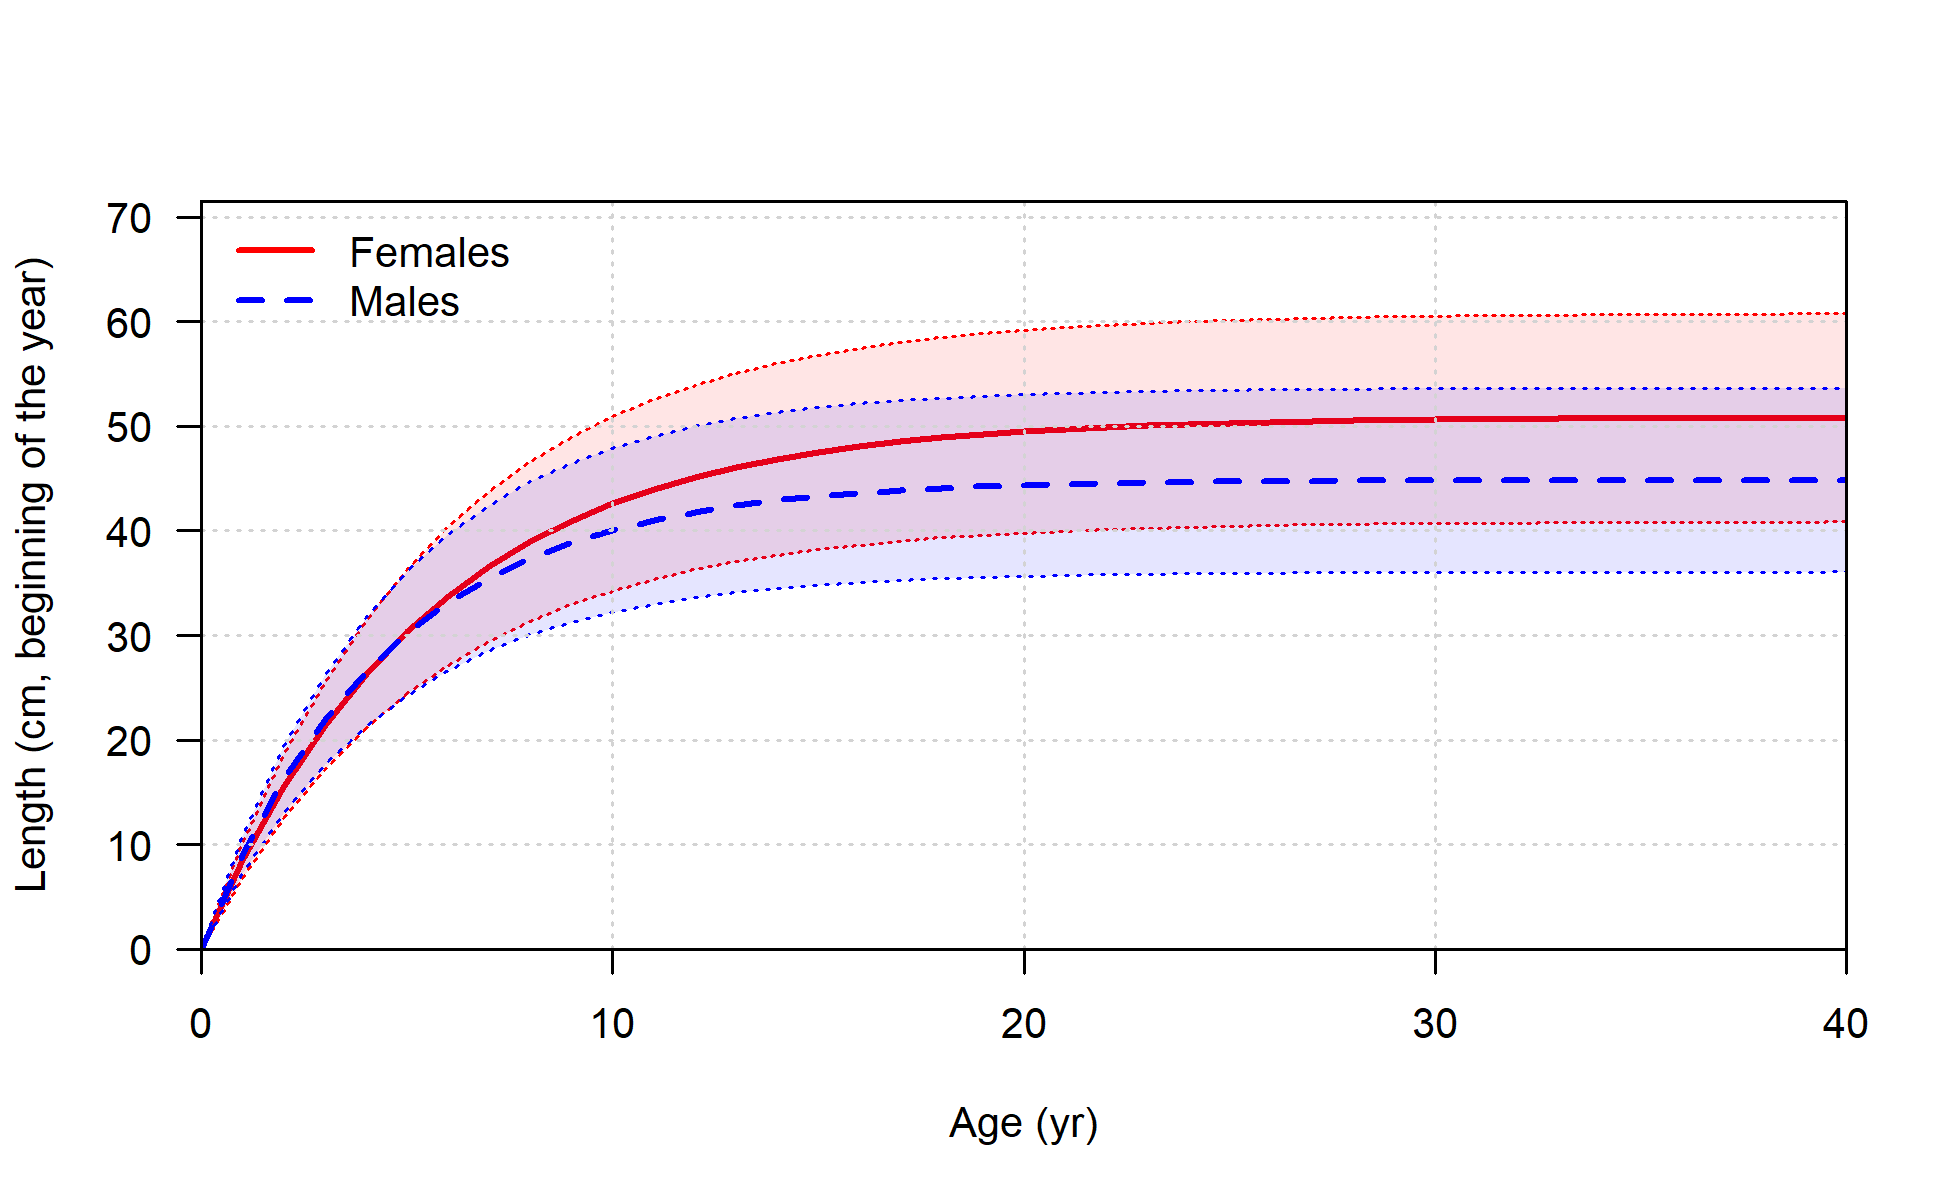
\includegraphics[width=1\textwidth,height=1\textheight]{C:/Users/Jason.Cope/Documents/Github/Sebastes_melanops_OR/Document/models/Reference model/plots/bio1_sizeatage.png}
\caption{Model estimated length-at-age in the beginning of the year. Shaded area indicates 95 percent distribution of length-at-age around the estimated growth curve.\label{fig:len-age-ss}}
\end{figure}

\begin{figure}
\centering
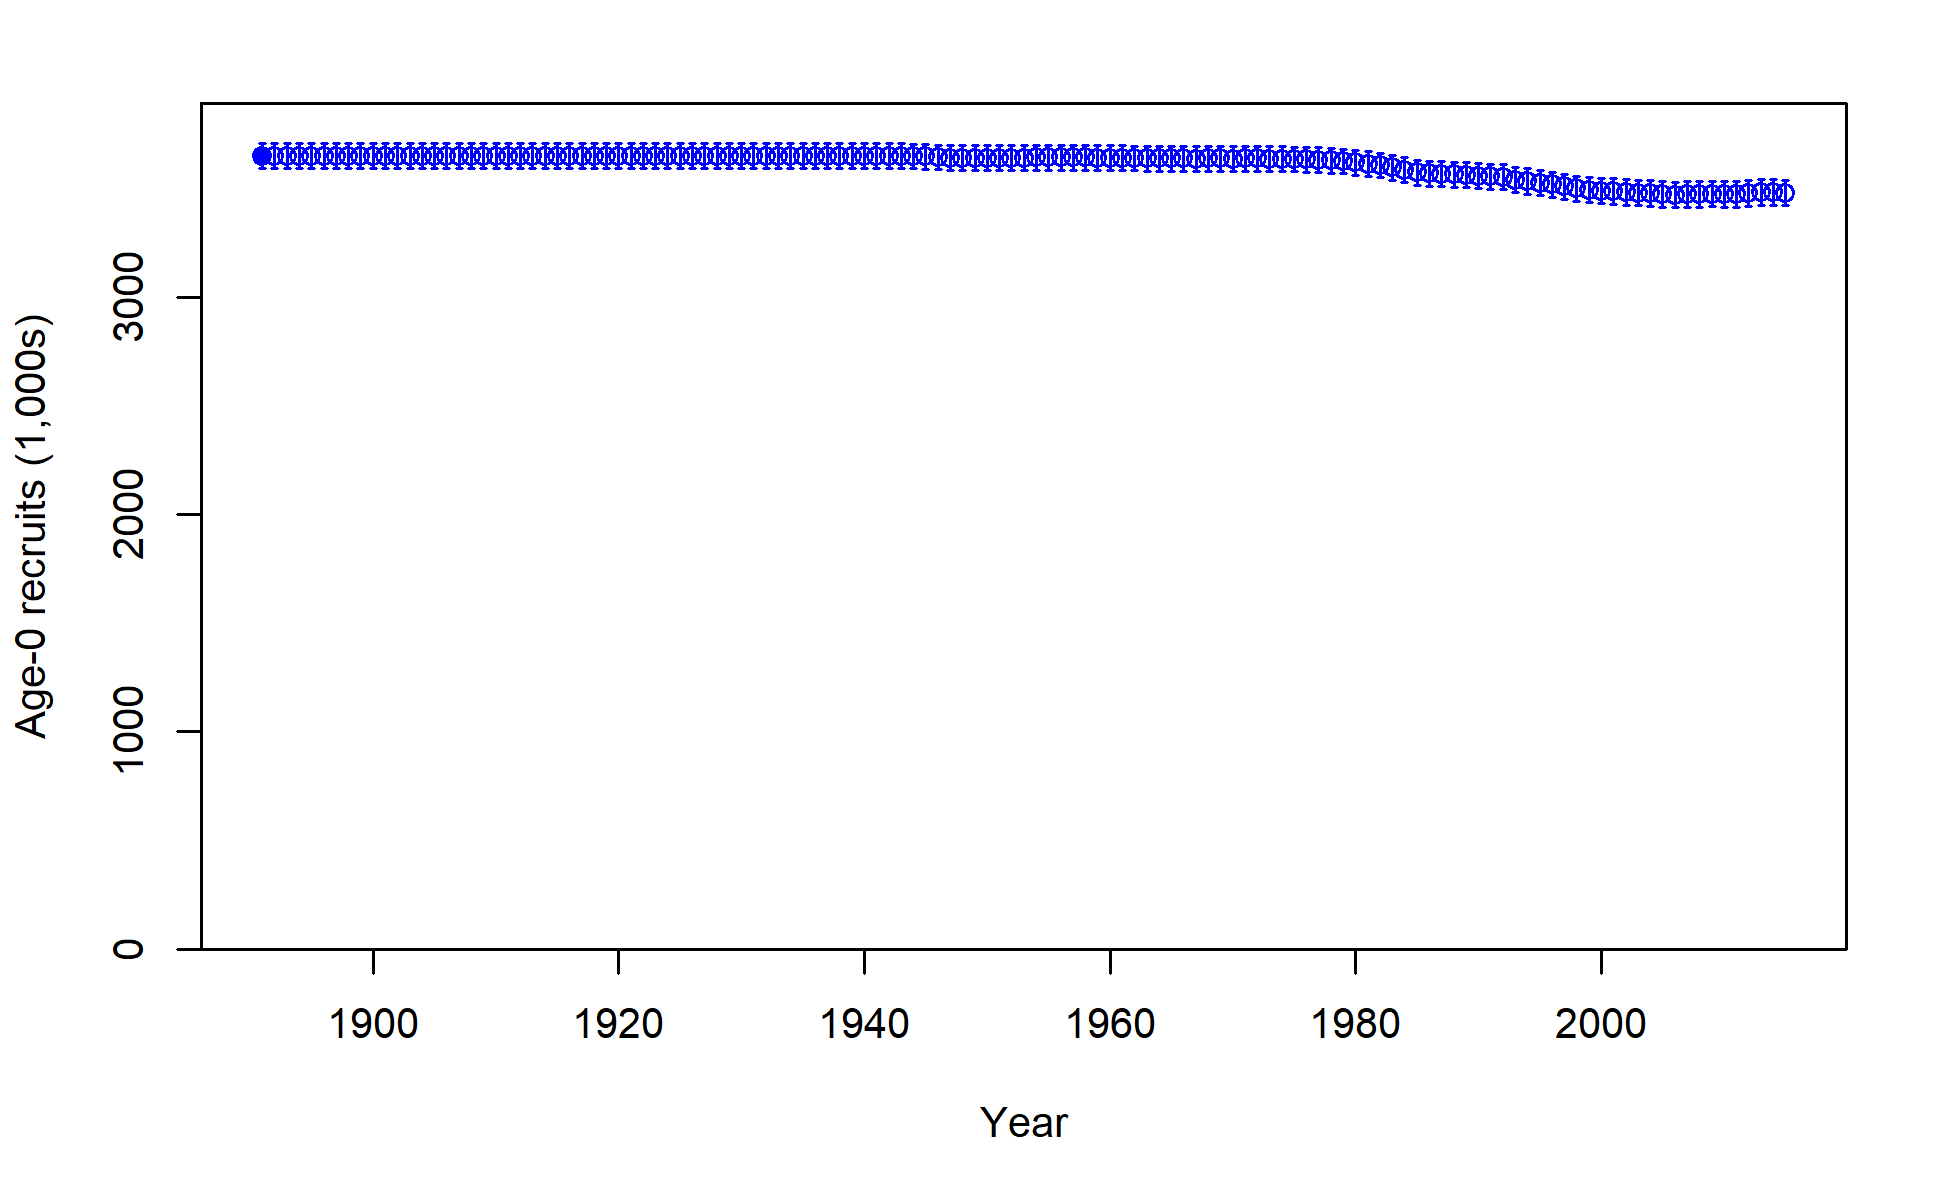
\includegraphics[width=1\textwidth,height=1\textheight]{C:/Users/Jason.Cope/Documents/Github/Sebastes_melanops_OR/Document/models/Reference model/plots/ts11_Age-0_recruits_(1000s)_with_95_asymptotic_intervals.png}
\caption{Estimated time series of age-0 recruits (1000s).\label{fig:recruits}}
\end{figure}

\begin{figure}
\centering
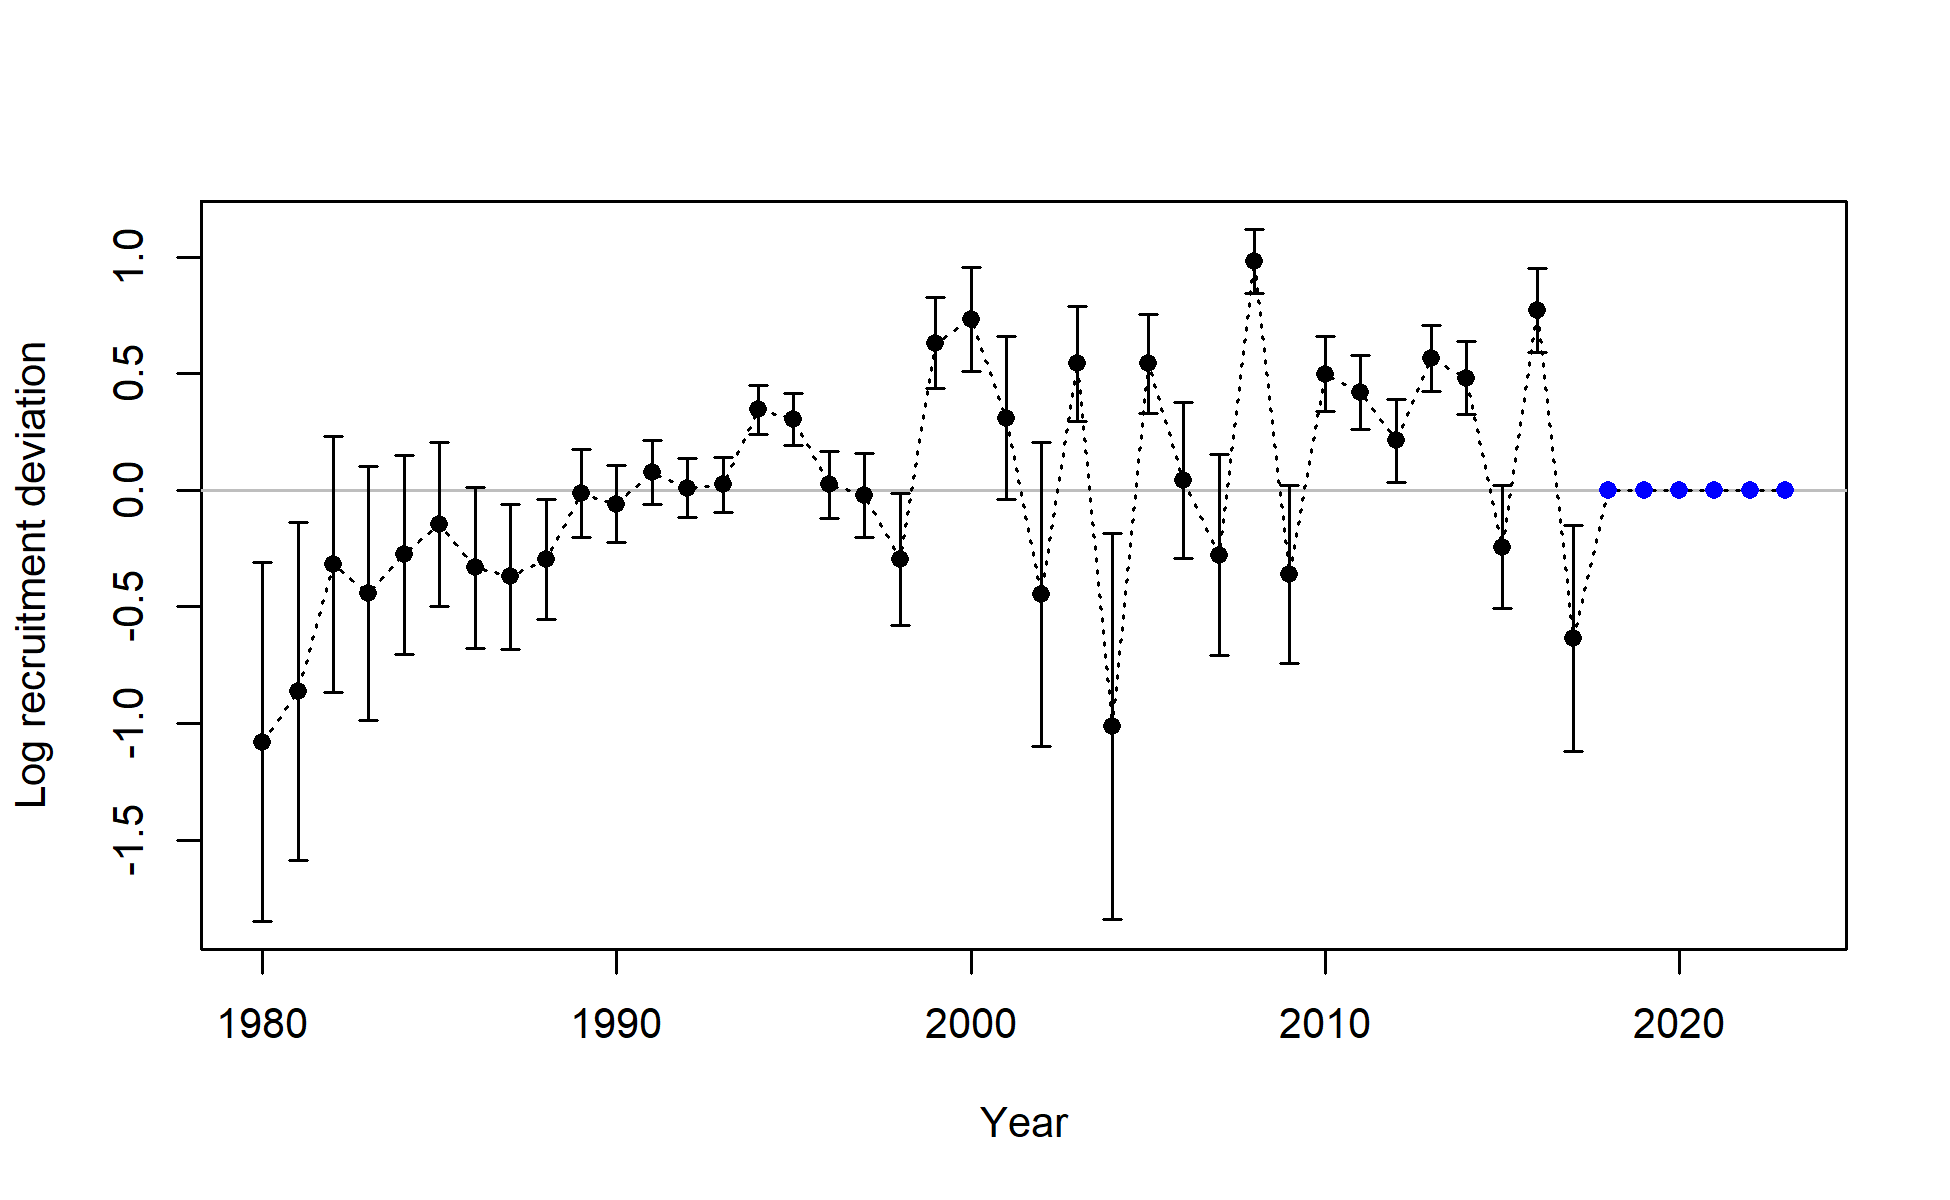
\includegraphics[width=1\textwidth,height=1\textheight]{C:/Users/Jason.Cope/Documents/Github/Sebastes_melanops_OR/Document/models/Reference model/plots/recdevs2_withbars.png}
\caption{Estimated time series of recruitment deviations.\label{fig:rec-devs}}
\end{figure}

\begin{figure}
\centering
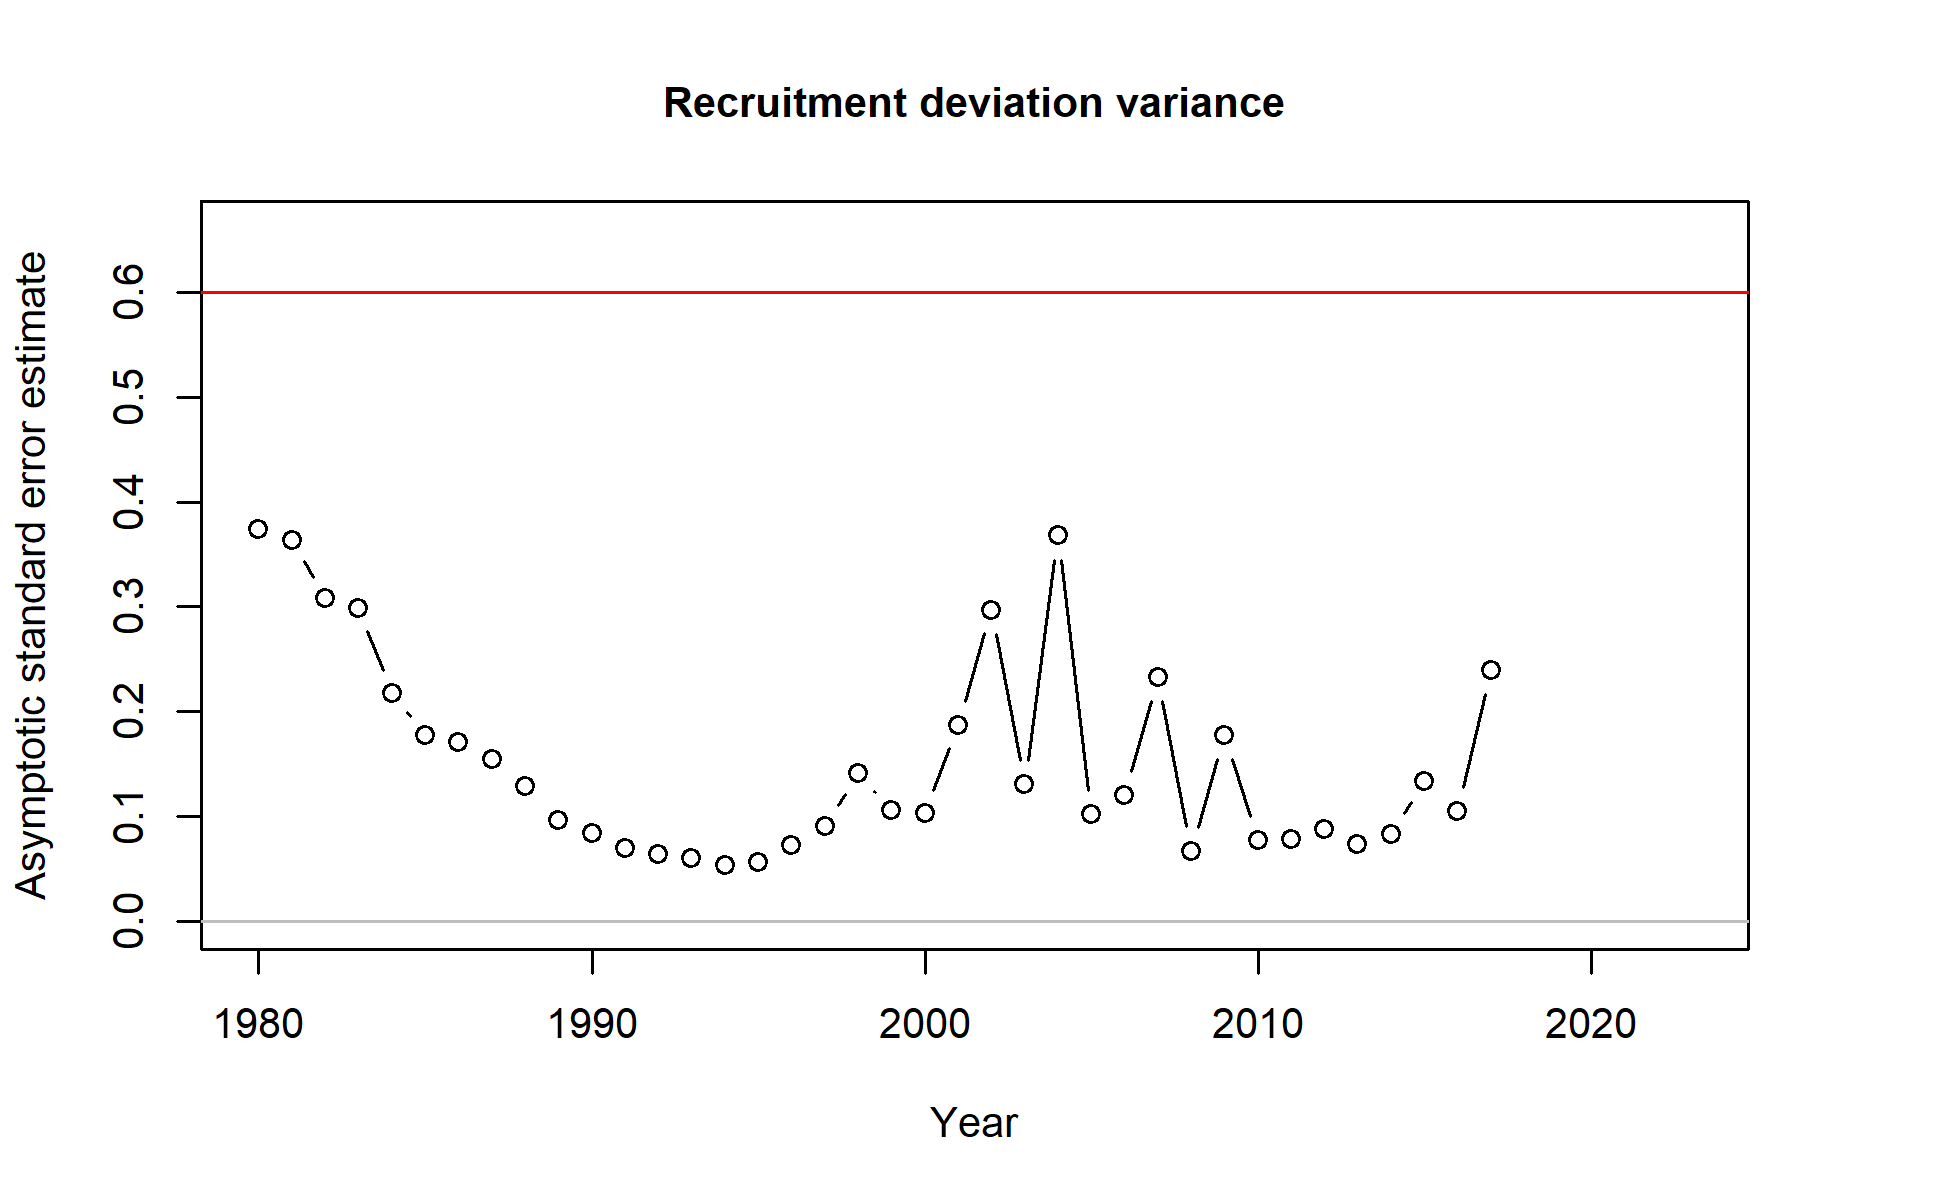
\includegraphics[width=1\textwidth,height=1\textheight]{C:/Users/Jason.Cope/Documents/Github/Sebastes_melanops_OR/Document/models/Reference model/plots/recdevs3_varcheck.png}
\caption{Recruitment deviations variance by year. This plot tracks the information content contained in each recruitment deviation. Values below the red line (assumed recruitment variability) indicates years with more informed recruitment deviations.\label{fig:rec-devs-sigmas}}
\end{figure}

\begin{figure}
\centering
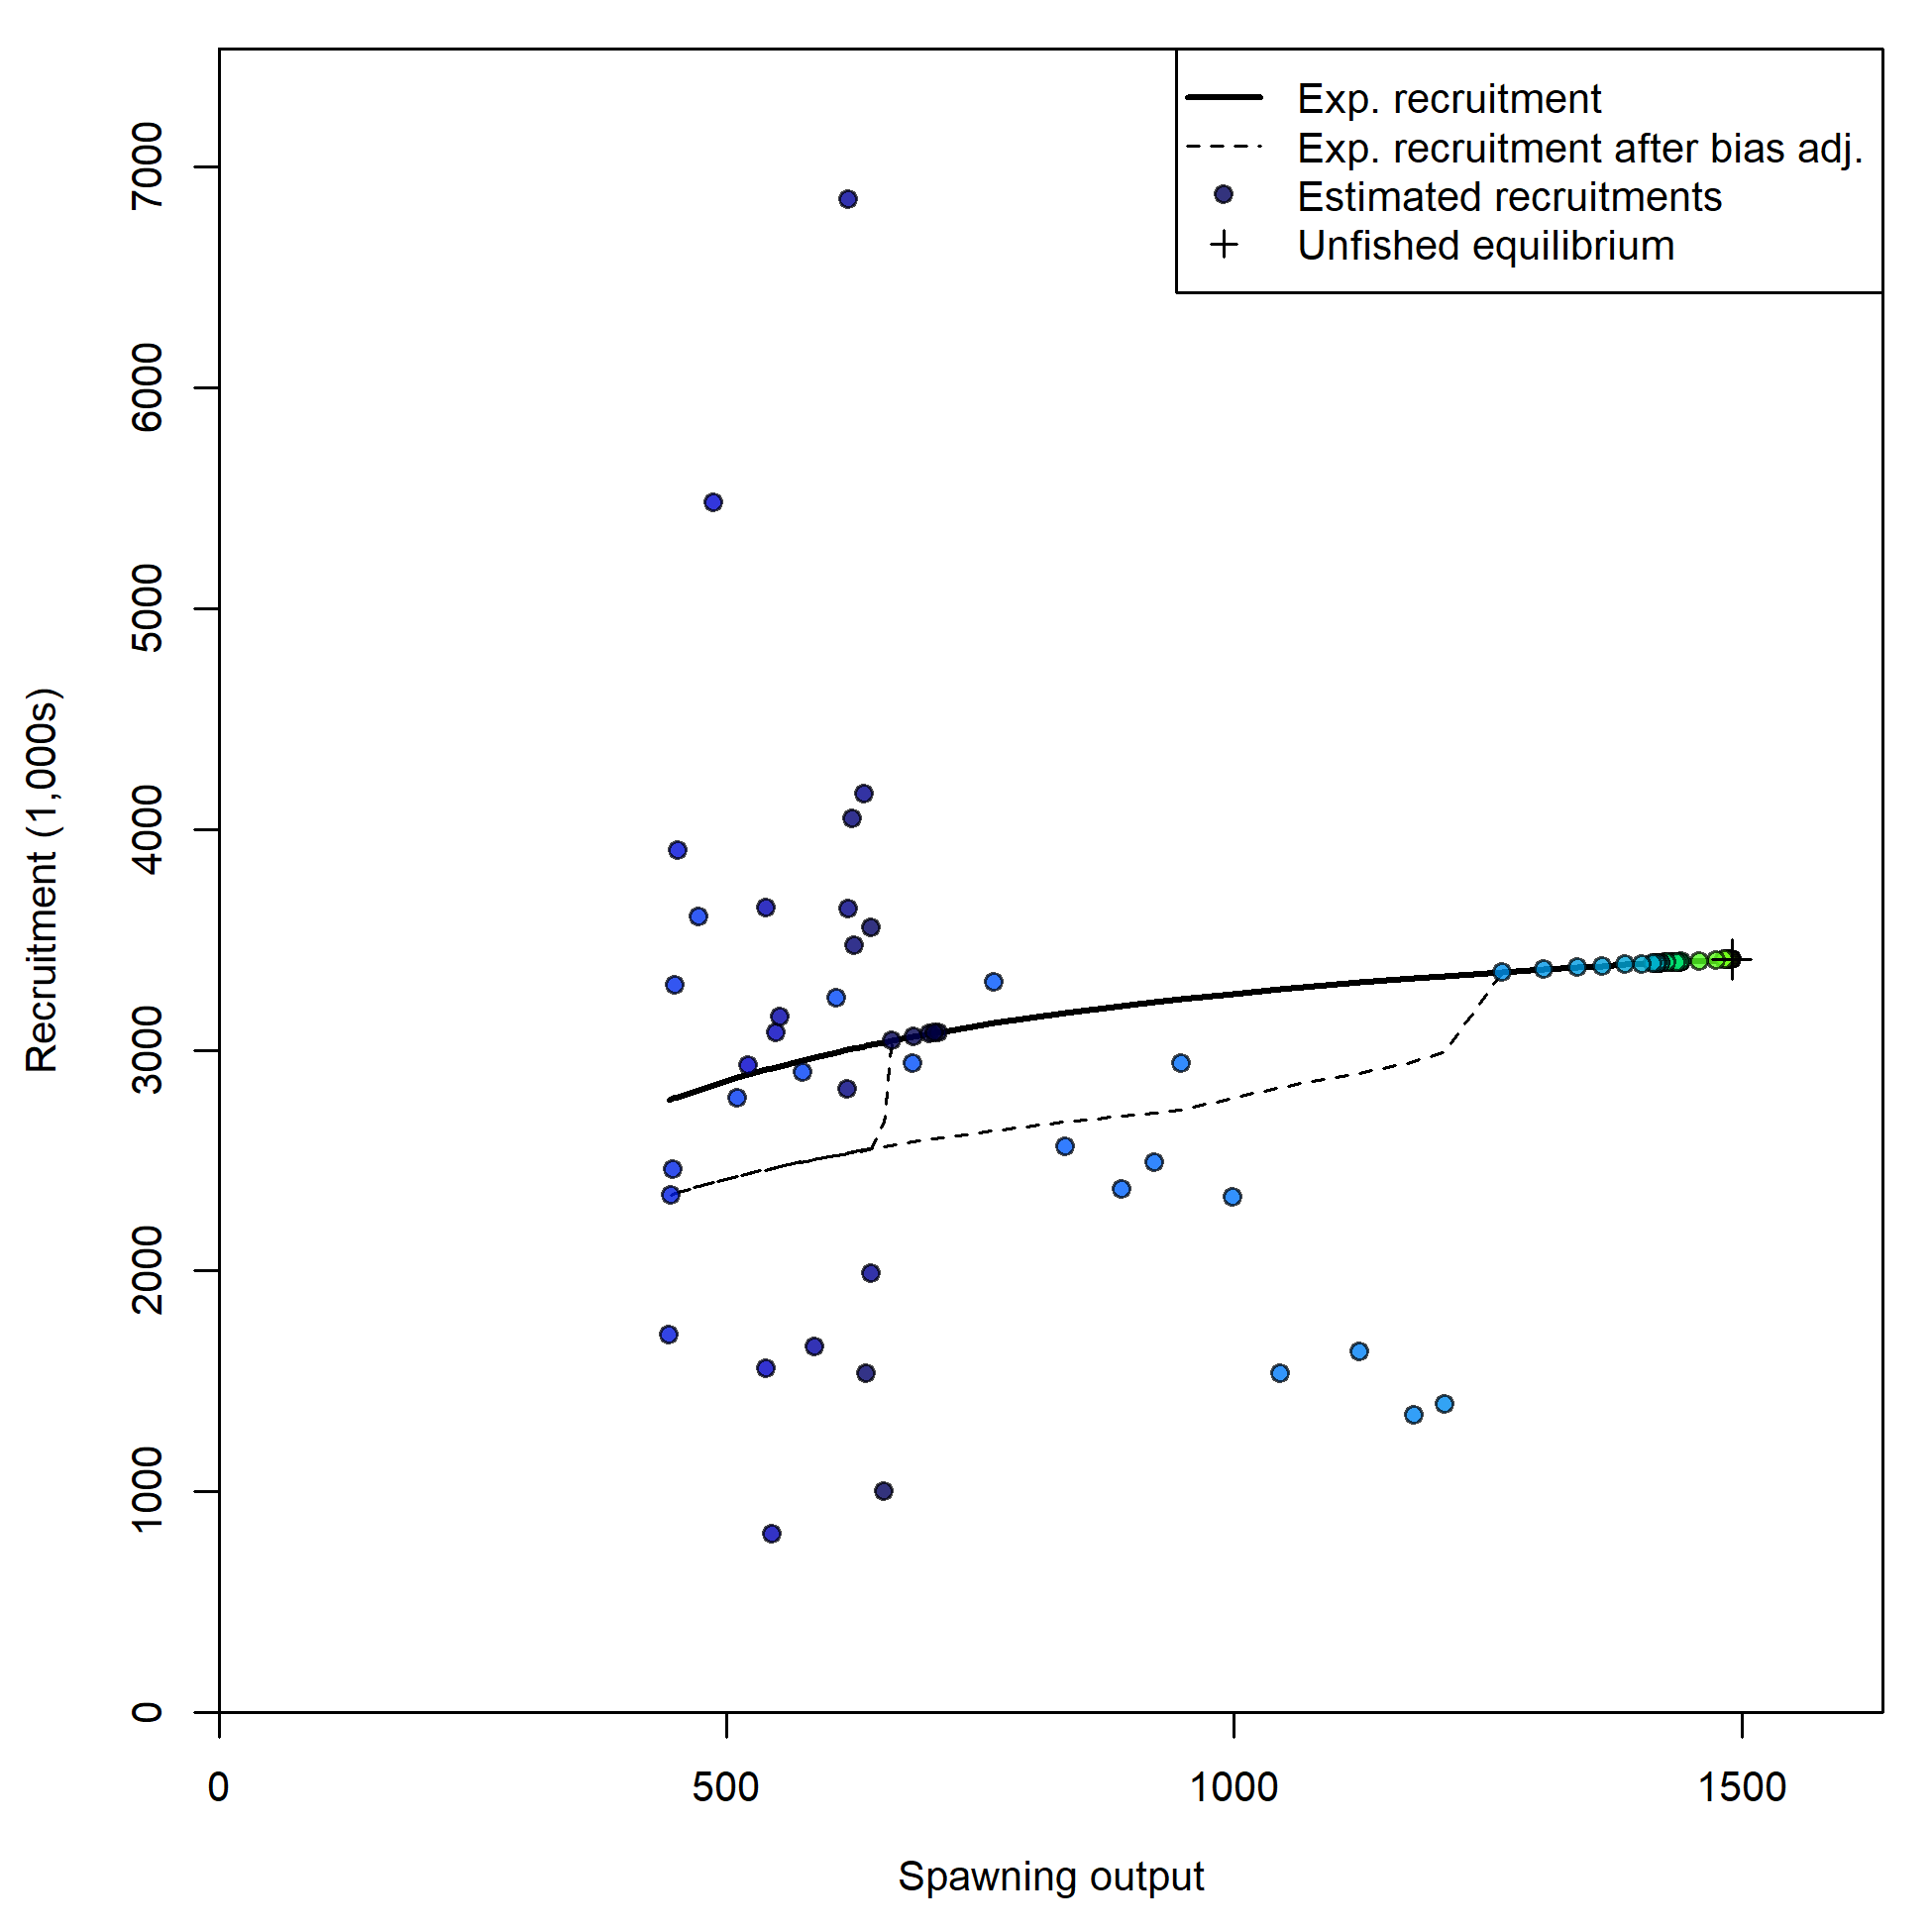
\includegraphics[width=1\textwidth,height=1\textheight]{C:/Users/Jason.Cope/Documents/Github/Sebastes_melanops_OR/Document/models/Reference model/plots/SR_curve.png}
\caption{Stock-recruit curve. Point colors indicate year, with warmer colors indicating earlier years and cooler colors in showing later years.\label{fig:bh-curve}}
\end{figure}

\begin{figure}
\centering
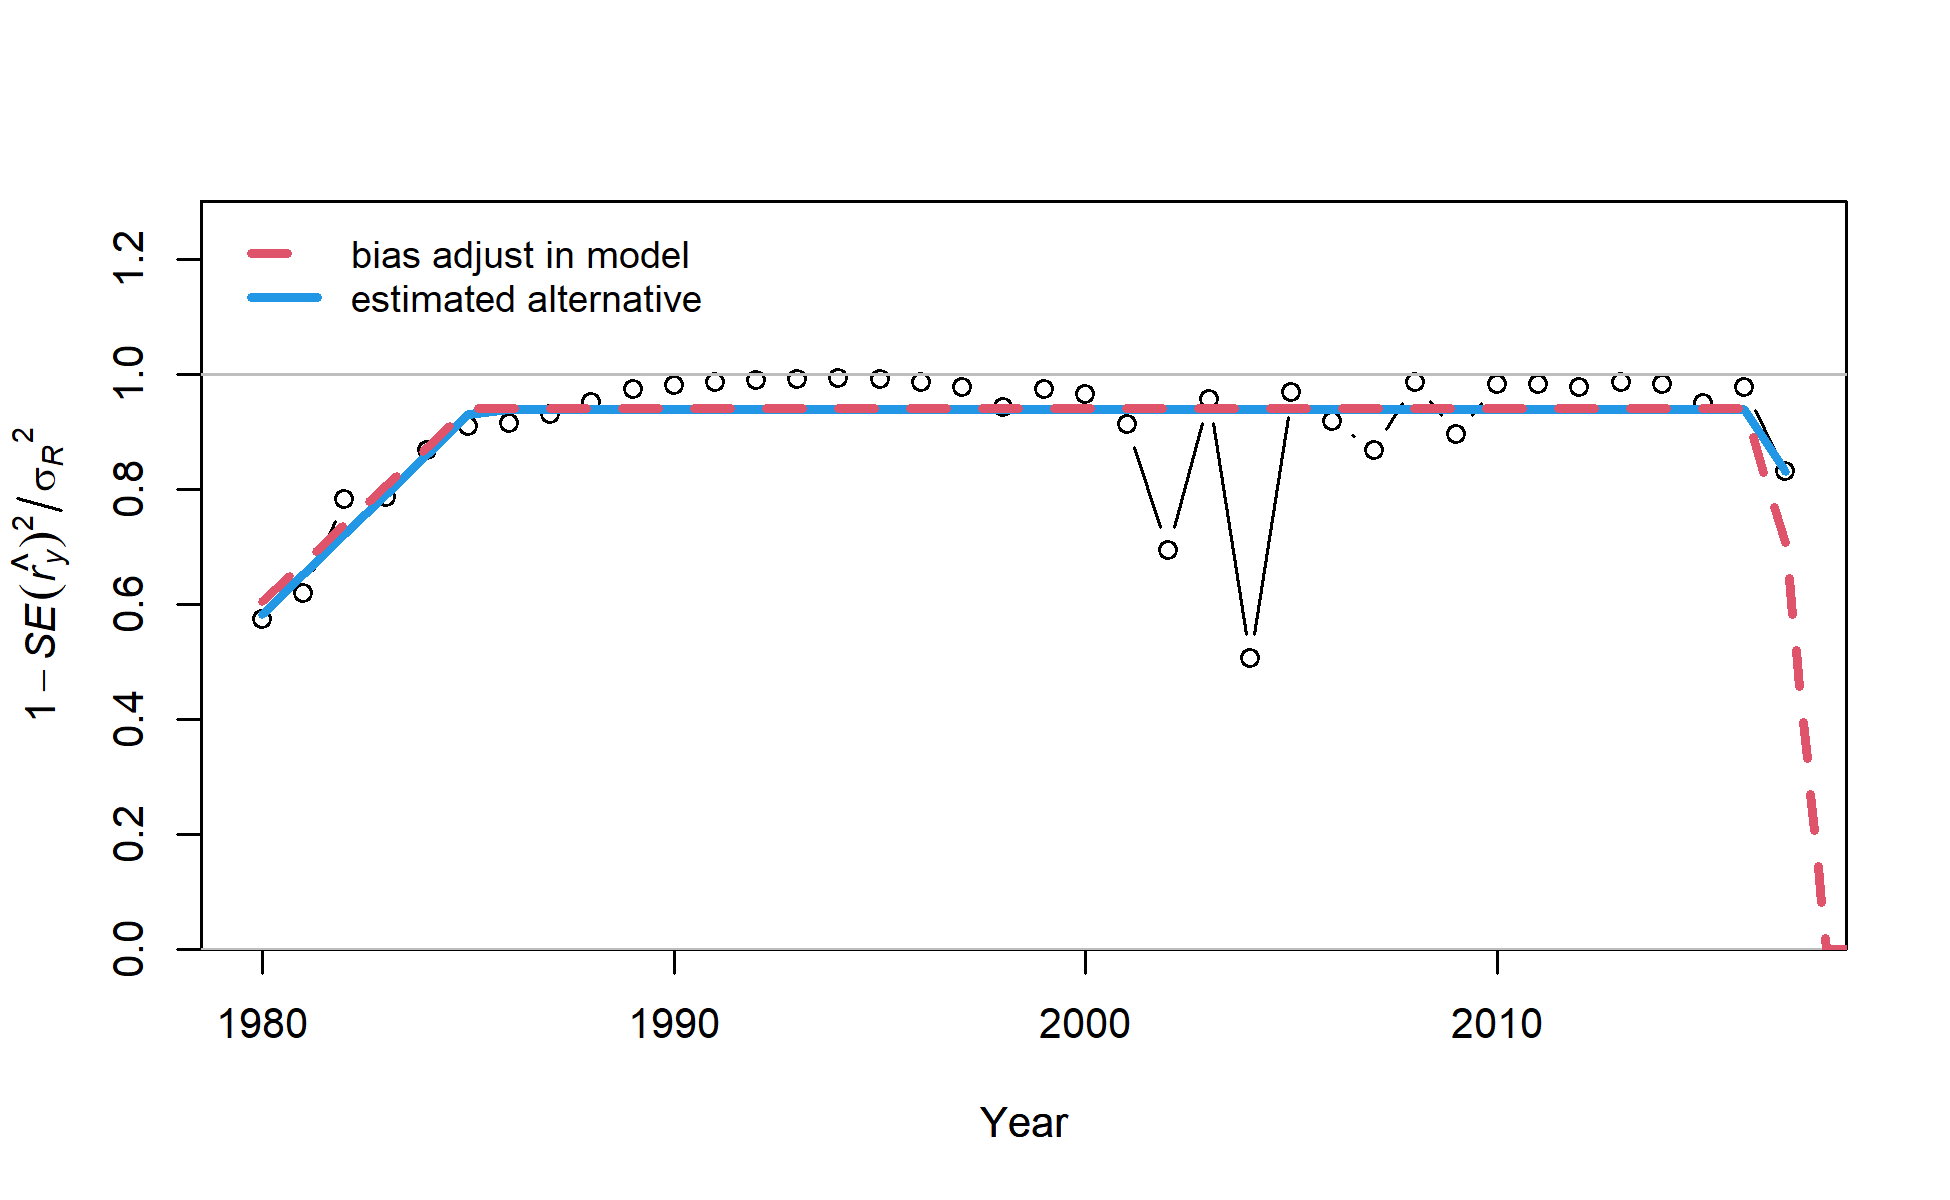
\includegraphics[width=1\textwidth,height=1\textheight]{C:/Users/Jason.Cope/Documents/Github/Sebastes_melanops_OR/Document/models/Reference model/plots/recruit_fit_bias_adjust.png}
\caption{Recruitment bias adjustment applied in the reference model.\label{fig:bias-adj}}
\end{figure}

\begin{figure}
\centering
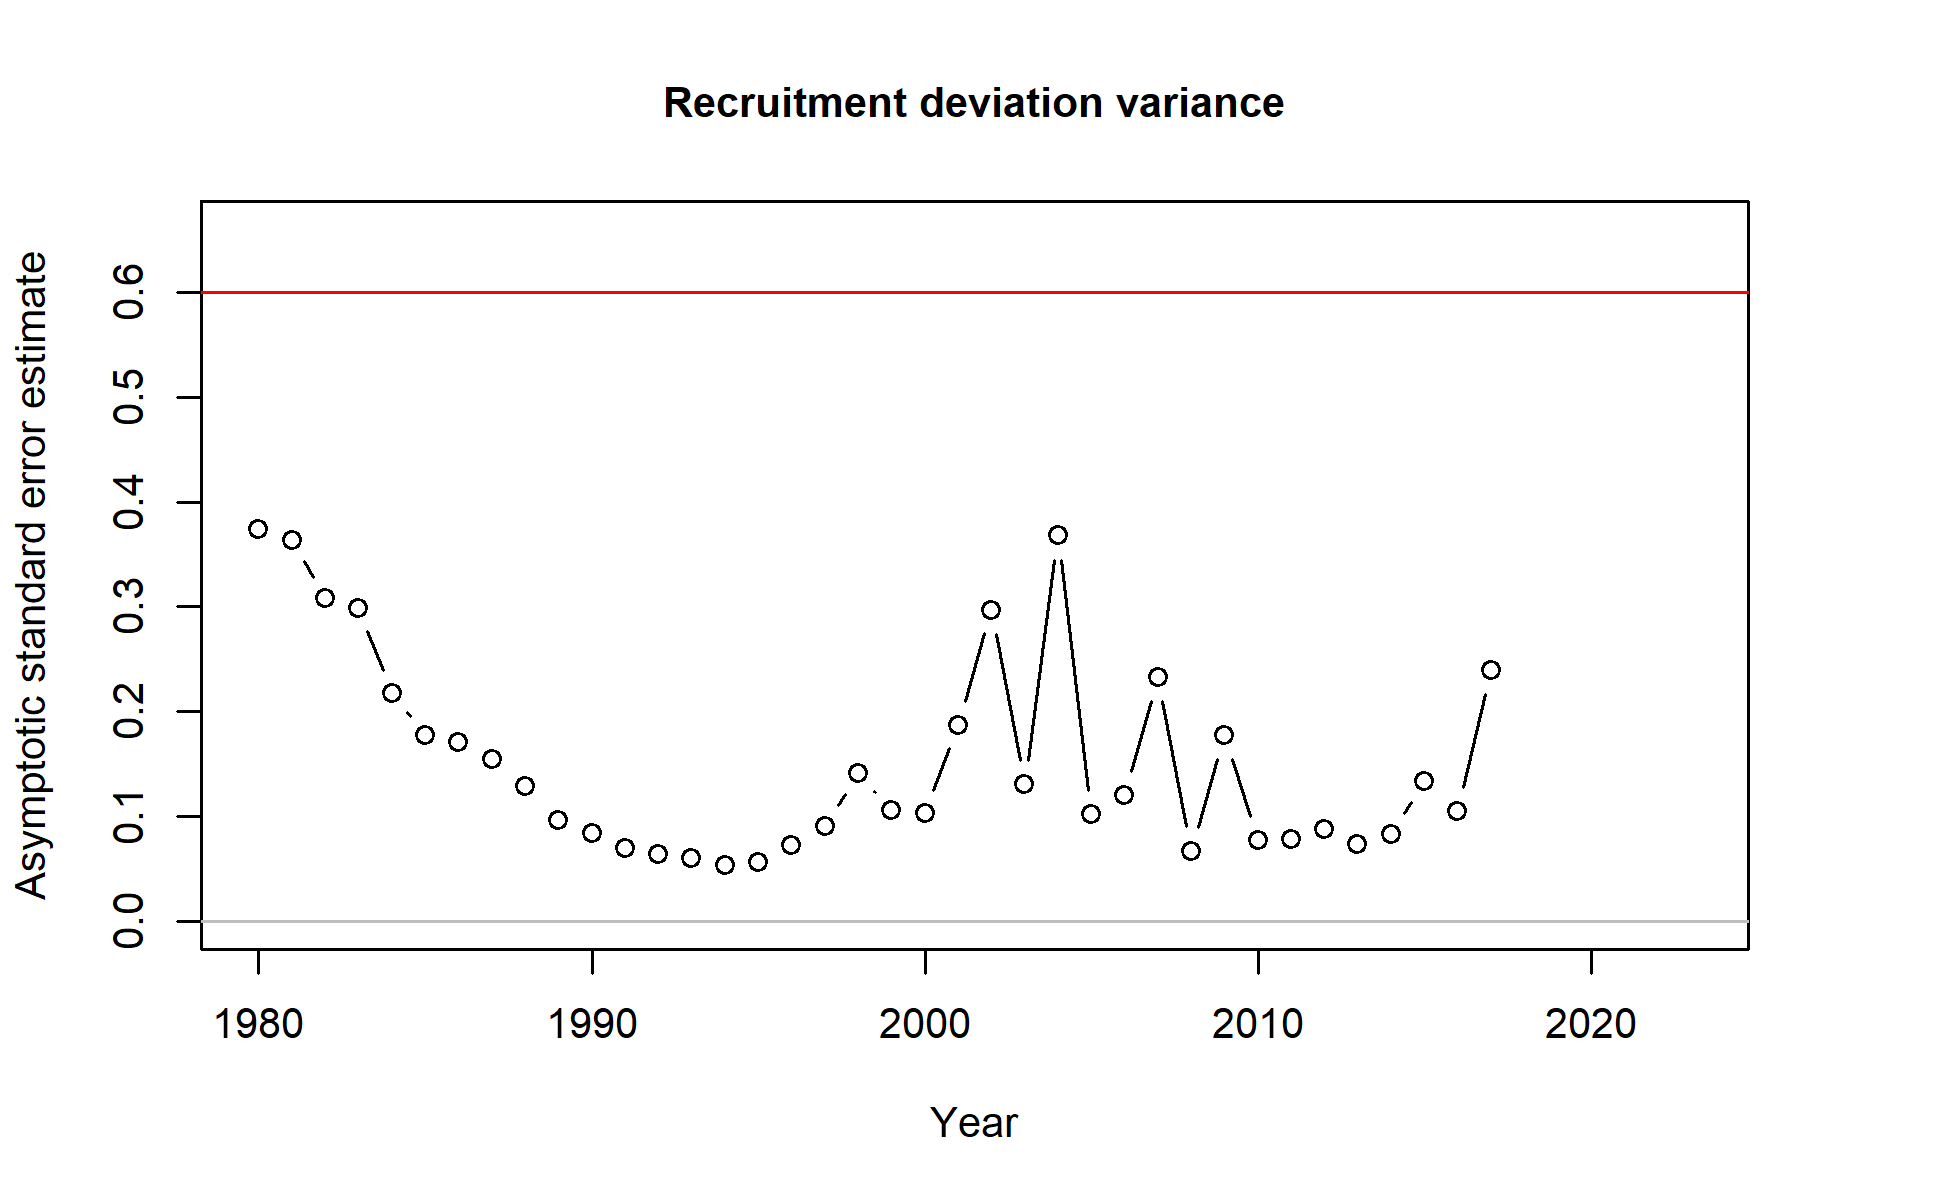
\includegraphics[width=1\textwidth,height=1\textheight]{C:/Users/Jason.Cope/Documents/Github/Sebastes_melanops_OR/Document/models/Reference model/plots/recdevs3_varcheck.png}
\caption{Recruitment deviations variance check. Low standard deviations indicate years with informative deviations .\label{fig:varcheck}}
\end{figure}

\begin{figure}
\centering
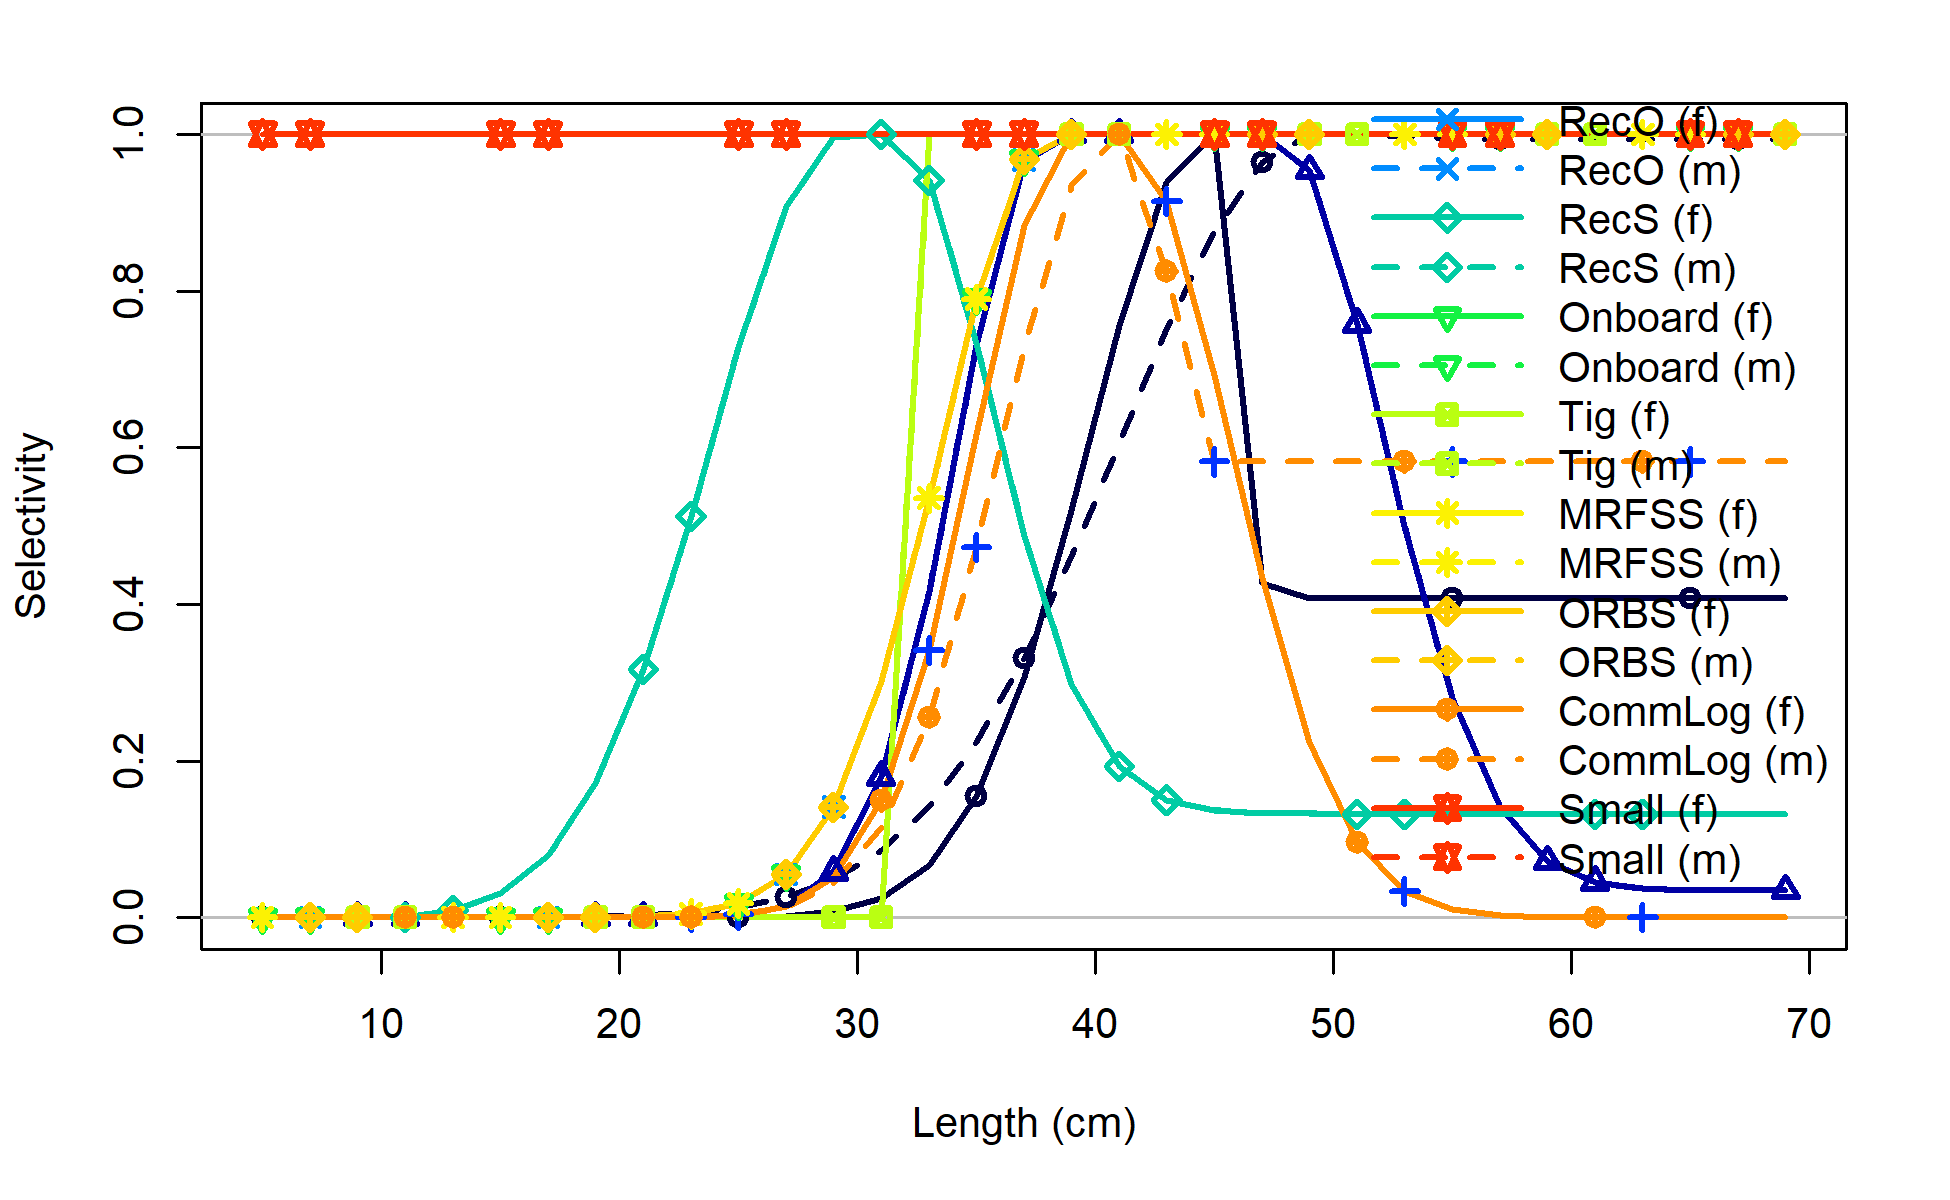
\includegraphics[width=1\textwidth,height=1\textheight]{C:/Users/Jason.Cope/Documents/Github/Sebastes_melanops_OR/Document/models/Reference model/plots/sel01_multiple_fleets_length1.png}
\caption{Length-based selectivity curves for each fleet and survey.\label{fig:fleet_selectivity}}
\end{figure}

\begin{figure}
\centering
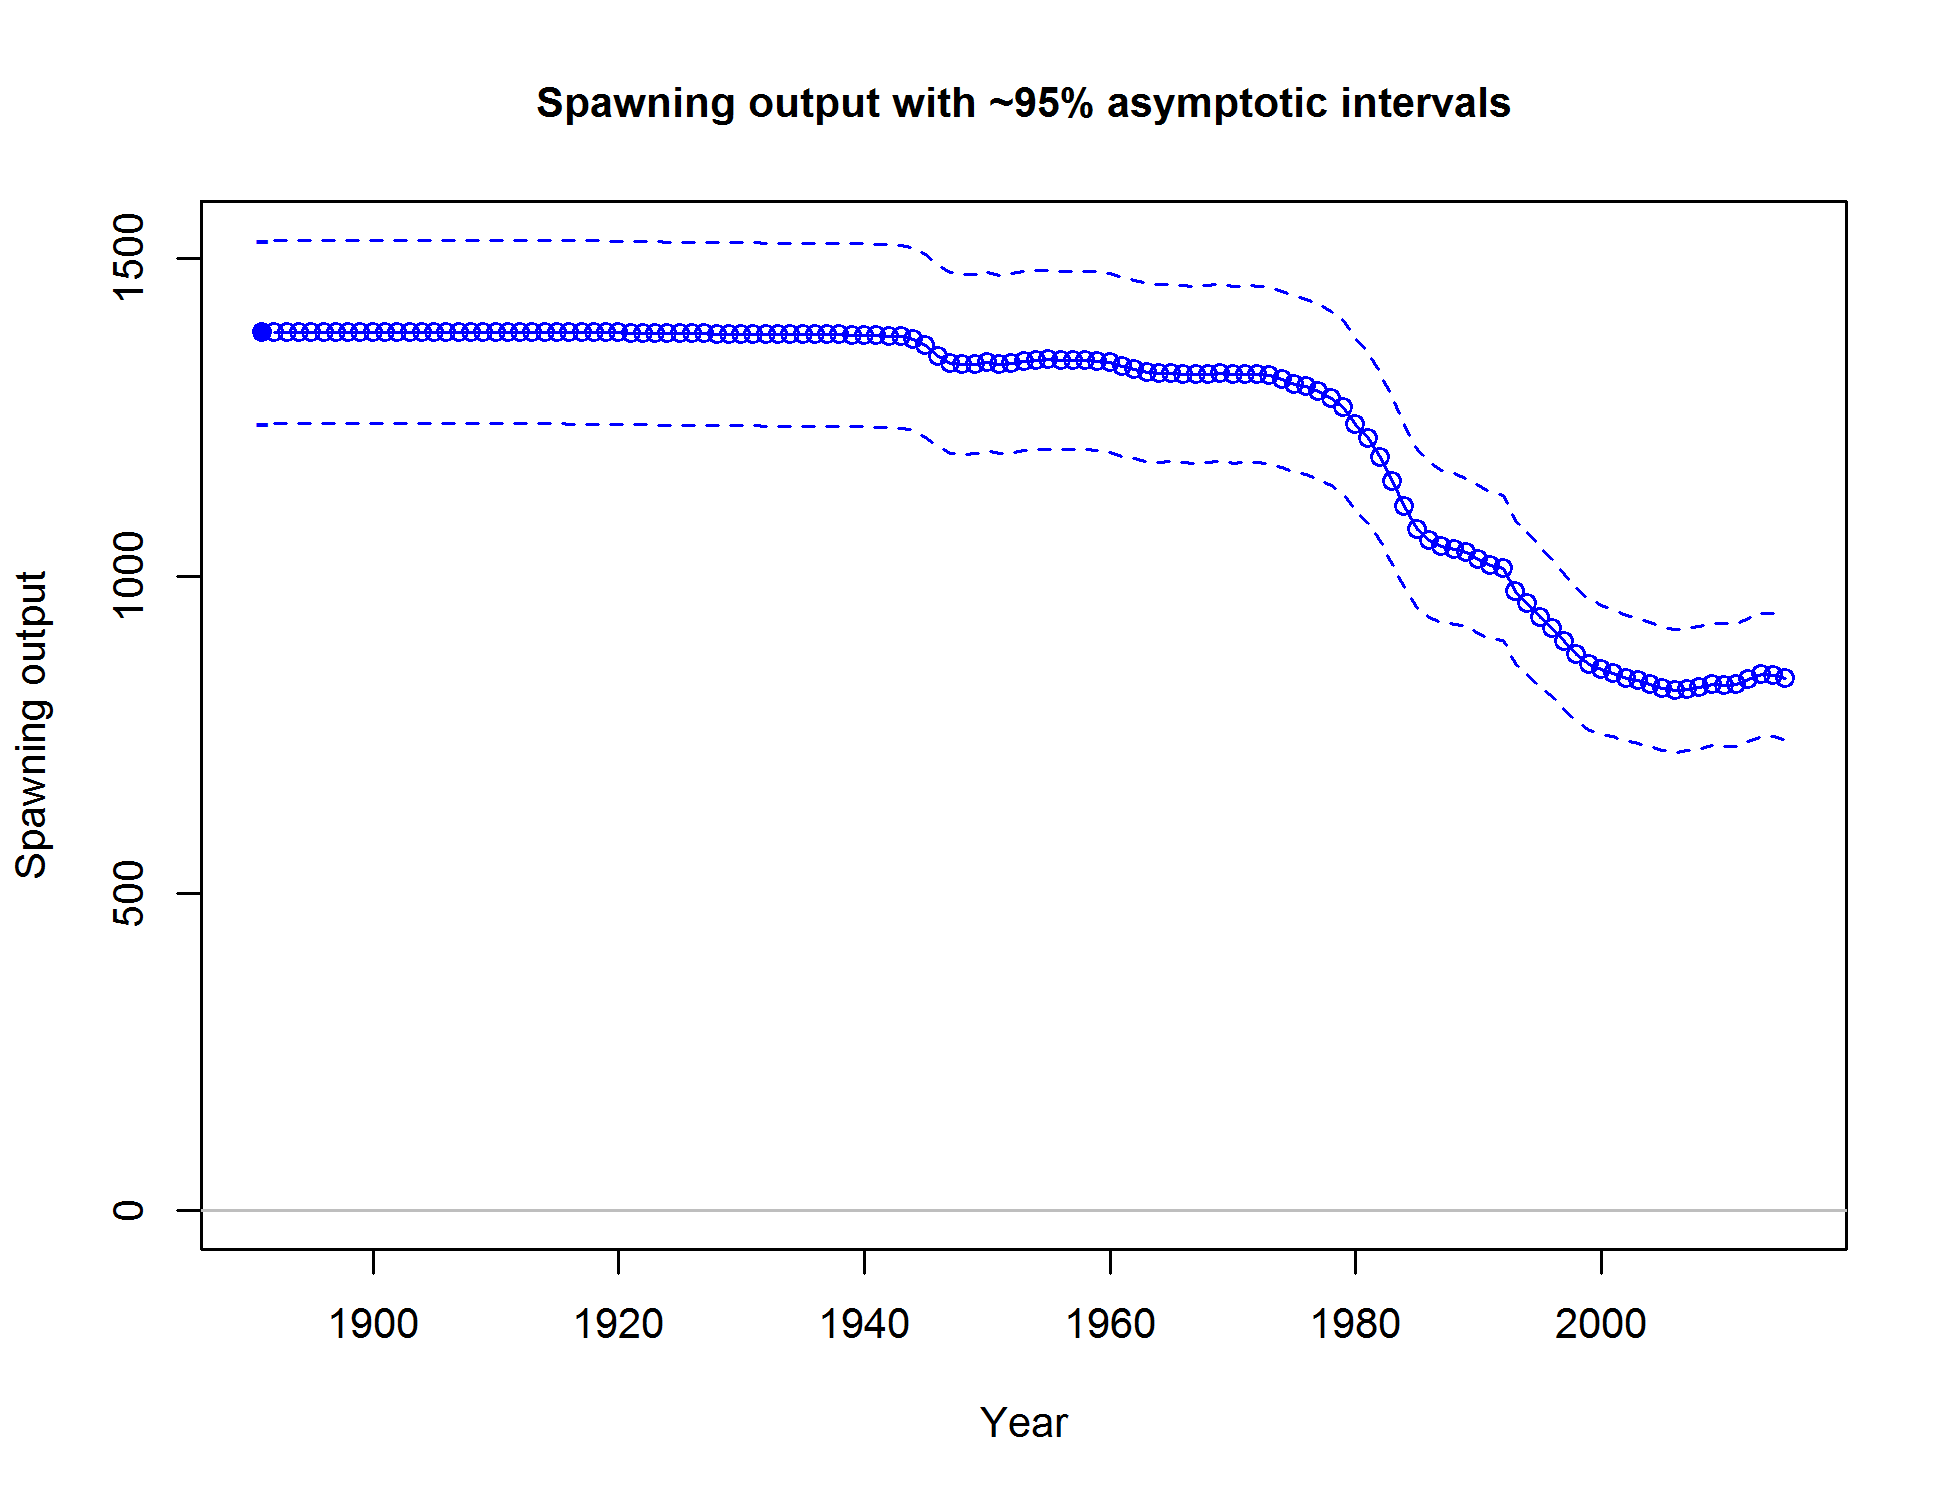
\includegraphics[width=1\textwidth,height=1\textheight]{C:/Users/Jason.Cope/Documents/Github/Sebastes_melanops_OR/Document/models/Reference model/plots/ts7_Spawning_output_with_95_asymptotic_intervals_intervals.png}
\caption{Estimated time series of spawning output (in millions of eggs).\label{fig:ssb}}
\end{figure}

\begin{figure}
\centering
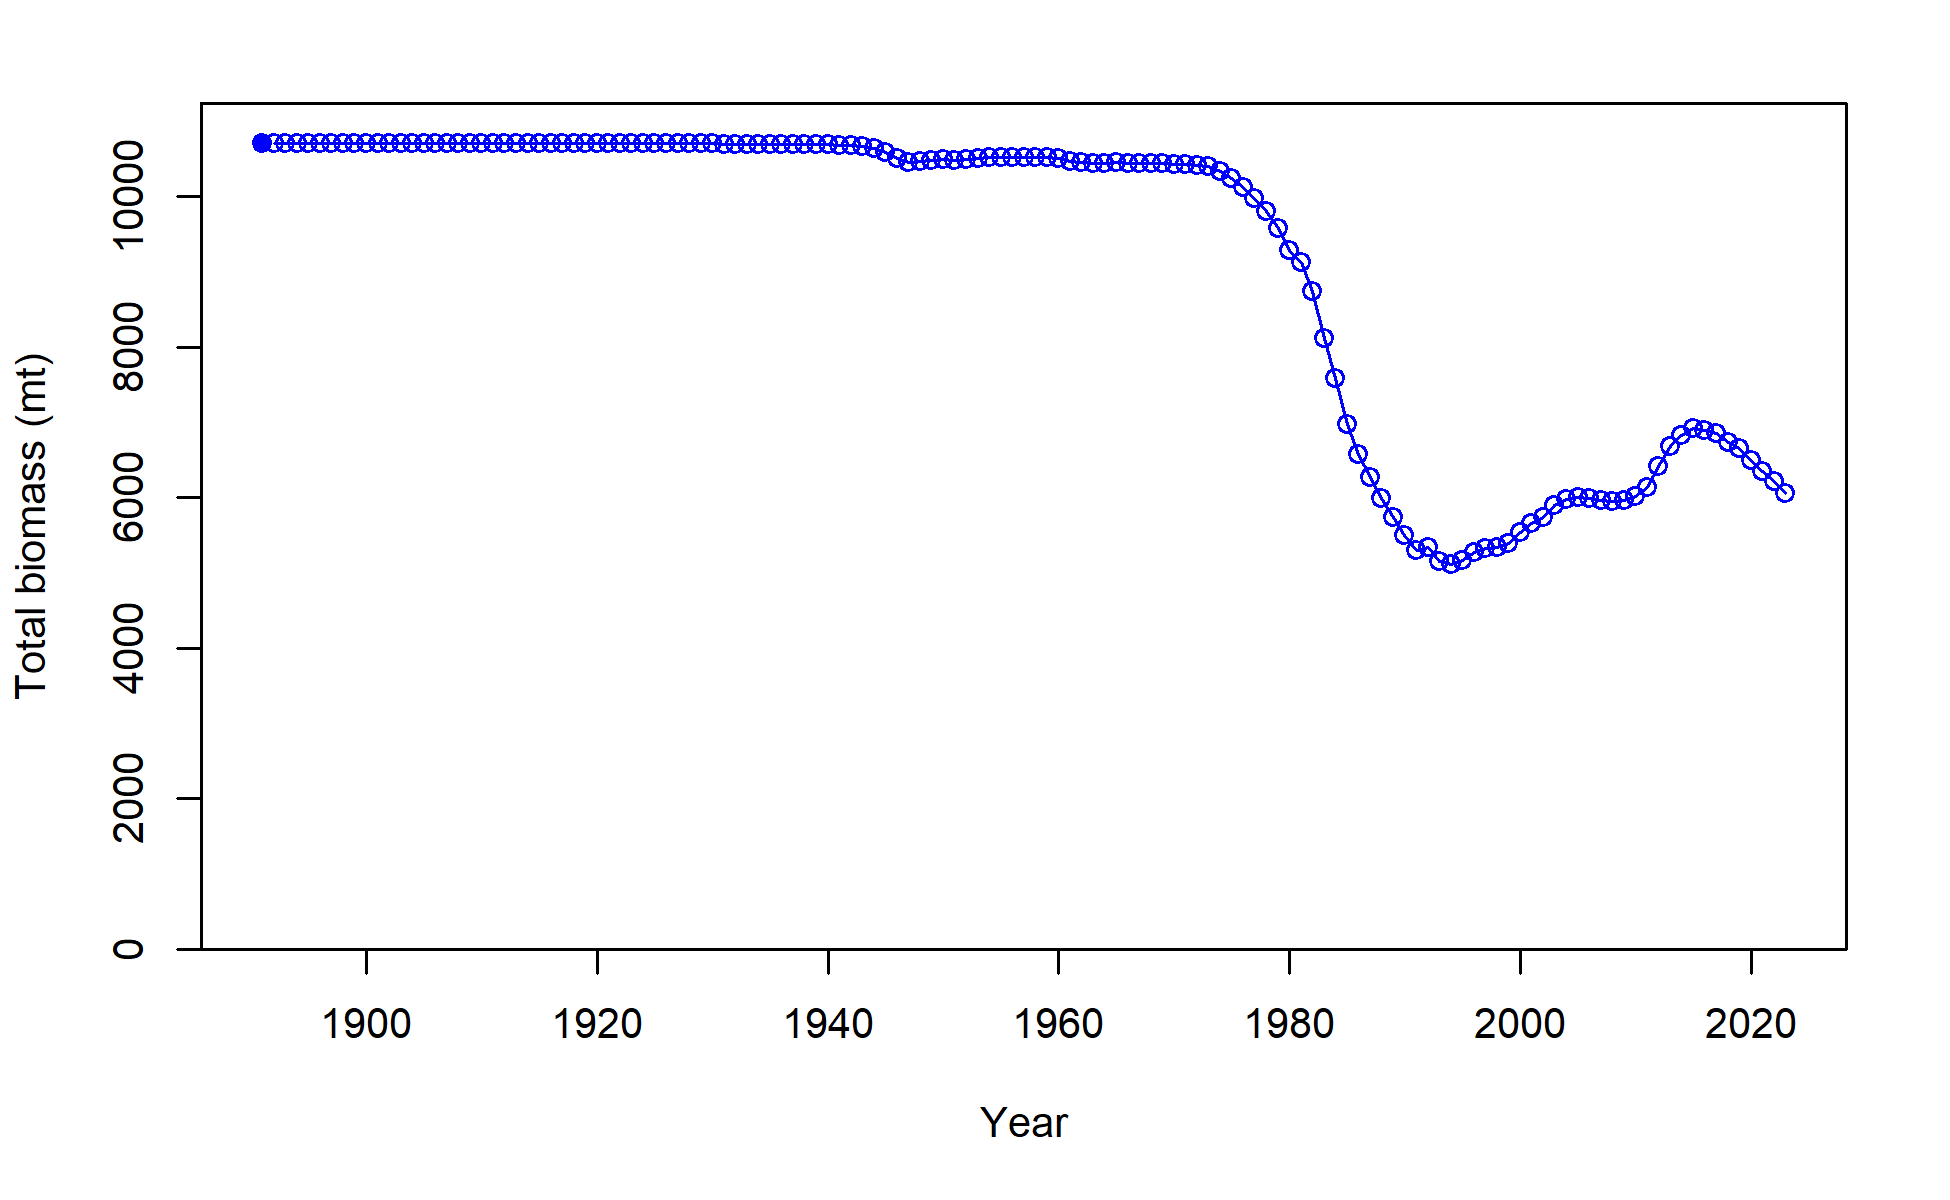
\includegraphics[width=1\textwidth,height=1\textheight]{C:/Users/Jason.Cope/Documents/Github/Sebastes_melanops_OR/Document/models/Reference model/plots/ts1_Total_biomass_(mt).png}
\caption{Estimated time series of total biomass (mt).\label{fig:tot-bio}}
\end{figure}

\begin{figure}
\centering
\includegraphics[width=1\textwidth,height=1\textheight]{C:/Users/Jason.Cope/Documents/Github/Sebastes_melanops_OR/Document/models/Reference model/plots/ts9_Relative_spawning_output_intervals.png}
\caption{Estimated time series of fraction of unfished spawning output.\label{fig:depl}}
\end{figure}

\begin{figure}
\centering
\includegraphics[width=1\textwidth,height=1\textheight]{C:/Users/Jason.Cope/Documents/Github/Sebastes_melanops_OR/Document/figures/comp_2015_2023/compare2_spawnbio_uncertainty.png}
\caption{Comparison of the time series of spawning output between the 2013 and 2023 assessment results.\label{fig:comp_ssb}}
\end{figure}

\begin{figure}
\centering
\includegraphics[width=1\textwidth,height=1\textheight]{C:/Users/Jason.Cope/Documents/Github/Sebastes_melanops_OR/Document/figures/comp_2015_2023/compare4_Bratio_uncertainty.png}
\caption{Comparison of the time series of relative spawning output between the 2013 and 2023 assessment results.\label{fig:comp_depl}}
\end{figure}

\begin{figure}
\centering
\includegraphics[width=1\textwidth,height=1\textheight]{C:/Users/Jason.Cope/Documents/Github/Sebastes_melanops_OR/Document/figures/likelihoods/parameter_panel_LnQ_base_Acoustic_Visual(6).png}
\caption{Acoustic-visual survey catchability likelihood profile (change in the negative log-likelihood across a range of \(ln(R0)\) values) and derived quantities. Red line in the top left figure indicates the significance level in likelihood difference.\label{fig:AVq-profile}}
\end{figure}

\begin{figure}
\centering
\includegraphics[width=1\textwidth,height=1\textheight]{C:/Users/Jason.Cope/Documents/Github/Sebastes_melanops_OR/Document/figures/likelihoods/piner_panel_LnQ_base_Acoustic_Visual(6).png}
\caption{Acoustic-visual survey catchability likelihood profile for each of the likelihood components.\label{fig:AVq-profile-components}}
\end{figure}

\begin{figure}
\centering
\includegraphics[width=1\textwidth,height=1\textheight]{C:/Users/Jason.Cope/Documents/Github/Sebastes_melanops_OR/Document/figures/likelihoods/parameter_panel_SR_BH_steep.png}
\caption{Beverton-Holt steepness parameter likelihood profile (change in the negative log-likelihood across a range of \(ln(R0)\) values) and derived quantities. Red line in the top left figure indicates the significance level in likelihood difference.\label{fig:steepness-profile}}
\end{figure}

\begin{figure}
\centering
\includegraphics[width=1\textwidth,height=1\textheight]{C:/Users/Jason.Cope/Documents/Github/Sebastes_melanops_OR/Document/figures/likelihoods/piner_panel_SR_BH_steep.png}
\caption{Beverton-Holt steepness parameter likelihood profile for each of the likelihood components.\label{fig:steepness-profile-components}}
\end{figure}

\begin{figure}
\centering
\includegraphics[width=1\textwidth,height=1\textheight]{C:/Users/Jason.Cope/Documents/Github/Sebastes_melanops_OR/Document/figures/likelihoods/M_fm_multilikelihood_profile.png}
\caption{Female and male \(M\) multi-parameter likelihood profile and derived quantities. Red lines in the top left figure indicate significantly similar values compared to the reference model. Broken and solid lines in the bottom right figure indicate target and limit referene points, respectively.\label{fig:M-multiprofile-combo}}
\end{figure}

\begin{figure}
\centering
\includegraphics[width=1\textwidth,height=1\textheight]{C:/Users/Jason.Cope/Documents/Github/Sebastes_melanops_OR/Document/figures/retro/compare2_spawnbio_uncertainty.png}
\caption{Change in the estimate of spawning output when the most recent 10 years of data area removed sequentially.\label{fig:retro-ssb}}
\end{figure}

\begin{figure}
\centering
\includegraphics[width=1\textwidth,height=1\textheight]{C:/Users/Jason.Cope/Documents/Github/Sebastes_melanops_OR/Document/figures/retro/compare4_Bratio_uncertainty.png}
\caption{Change in the estimate of fraction unfished when the most recent 10 years of data area removed sequentially.\label{fig:retro-depl}}
\end{figure}

\newpage

\begin{figure}
\centering
\includegraphics[width=1\textwidth,height=1\textheight]{C:/Users/Jason.Cope/Documents/Github/Sebastes_melanops_OR/Document/models/Reference model/plots/SPR2_minusSPRseries.png}
\caption{Estimated 1 - relative spawning ratio (SPR) by year.\label{fig:1-spr}}
\end{figure}

\clearpage

\begin{figure}
\centering
\includegraphics[width=1\textwidth,height=1\textheight]{C:/Users/Jason.Cope/Documents/Github/Sebastes_melanops_OR/Document/models/Reference model/plots/SPR4_phase.png}
\caption{Phase plot of the relative biomass (also referred to as fraction unfished) versus the SPR ratio where each point represents the biomass ratio at the start of the year and the relative fishing intensity in that same year. Lines through the final point show the 95 percent intervals based on the asymptotic uncertainty for each dimension. The shaded ellipse is a 95 percent region which accounts for the estimated correlations between the biomass ratio and SPR ratio.\label{fig:phase}}
\end{figure}

\begin{figure}
\centering
\includegraphics[width=1\textwidth,height=1\textheight]{C:/Users/Jason.Cope/Documents/Github/Sebastes_melanops_OR/Document/models/Reference model/plots/yield2_yield_curve_with_refpoints.png}
\caption{Equilibrium yield curve for the reference model. Values are based on the 2020 fishery selectivities and with steepness fixed at 0.72.\label{fig:yield}}
\end{figure}

\clearpage

\hypertarget{app-a}{%
\section{Appendix A: Detailed Fit to Length Composition Data}\label{app-a}}

\begin{figure}
\centering
\includegraphics[width=1\textwidth,height=1\textheight]{C:/Users/Jason.Cope/Documents/Github/Sebastes_melanops_OR/Document/models/Reference model/plots/comp_lenfit_flt1mkt0.png}
\caption{Length comps, whole catch, Trawl\_wdis.`N adj.' is the input sample size after data-weighting adjustment. N eff. is the calculated effective sample size used in the McAllister-Ianelli tuning method.\label{fig:comp_lenfit_flt1mkt0}}
\end{figure}

\begin{figure}
\centering
\includegraphics[width=1\textwidth,height=1\textheight]{C:/Users/Jason.Cope/Documents/Github/Sebastes_melanops_OR/Document/models/Reference model/plots/comp_lenfit_flt2mkt0_page1.png}
\caption{Length comps, whole catch, Non-Trawl\_wdis (plot 1 of 2).`N adj.' is the input sample size after data-weighting adjustment. N eff. is the calculated effective sample size used in the McAllister-Ianelli tuning method.\label{fig:comp_lenfit_flt2mkt0_page1}}
\end{figure}

\begin{figure}
\centering
\includegraphics[width=1\textwidth,height=1\textheight]{C:/Users/Jason.Cope/Documents/Github/Sebastes_melanops_OR/Document/models/Reference model/plots/comp_lenfit_flt2mkt0_page2.png}
\caption{Length comps, whole catch, Non-Trawl\_wdis (plot 1 of 2).`N adj.' is the input sample size after data-weighting adjustment. N eff. is the calculated effective sample size used in the McAllister-Ianelli tuning method. (plot 2 of 2).\label{fig:comp_lenfit_flt2mkt0_page2}}
\end{figure}

\begin{figure}
\centering
\includegraphics[width=1\textwidth,height=1\textheight]{C:/Users/Jason.Cope/Documents/Github/Sebastes_melanops_OR/Document/models/Reference model/plots/comp_lenfit_flt3mkt0_page1.png}
\caption{Length comps, whole catch, Ocean (plot 1 of 2).`N adj.' is the input sample size after data-weighting adjustment. N eff. is the calculated effective sample size used in the McAllister-Ianelli tuning method.\label{fig:comp_lenfit_flt3mkt0_page1}}
\end{figure}

\begin{figure}
\centering
\includegraphics[width=1\textwidth,height=1\textheight]{C:/Users/Jason.Cope/Documents/Github/Sebastes_melanops_OR/Document/models/Reference model/plots/comp_lenfit_flt3mkt0_page2.png}
\caption{Length comps, whole catch, Ocean (plot 1 of 2).`N adj.' is the input sample size after data-weighting adjustment. N eff. is the calculated effective sample size used in the McAllister-Ianelli tuning method. (plot 2 of 2).\label{fig:comp_lenfit_flt3mkt0_page2}}
\end{figure}

\begin{figure}
\centering
\includegraphics[width=1\textwidth,height=1\textheight]{C:/Users/Jason.Cope/Documents/Github/Sebastes_melanops_OR/Document/models/Reference model/plots/comp_lenfit_flt4mkt0.png}
\caption{Length comps, whole catch, Shore.`N adj.' is the input sample size after data-weighting adjustment. N eff. is the calculated effective sample size used in the McAllister-Ianelli tuning method.\label{fig:comp_lenfit_flt4mkt0}}
\end{figure}

\begin{figure}
\centering
\includegraphics[width=1\textwidth,height=1\textheight]{C:/Users/Jason.Cope/Documents/Github/Sebastes_melanops_OR/Document/models/Reference model/plots/comp_lenfit_flt5mkt0.png}
\caption{Length comps, whole catch, MPA.`N adj.' is the input sample size after data-weighting adjustment. N eff. is the calculated effective sample size used in the McAllister-Ianelli tuning method.\label{fig:comp_lenfit_flt5mkt0}}
\end{figure}

\clearpage

\hypertarget{app-b}{%
\section{Appendix B: Fit to Conditional-Age-at-Length Composition Data}\label{app-b}}

\begin{figure}
\centering
\includegraphics[width=1\textwidth,height=1\textheight]{C:/Users/Jason.Cope/Documents/Github/Sebastes_melanops_OR/Document/models/Reference model/plots/comp_condAALfit_residsflt1mkt0_page1.png}
\caption{Pearson residuals, whole catch, Trawl\_wdis (max=13.44) (plot 1 of 3).\label{fig:comp_condAALfit_residsflt1mkt0_page1}}
\end{figure}

\begin{figure}
\centering
\includegraphics[width=1\textwidth,height=1\textheight]{C:/Users/Jason.Cope/Documents/Github/Sebastes_melanops_OR/Document/models/Reference model/plots/comp_condAALfit_residsflt1mkt0_page2.png}
\caption{Pearson residuals, whole catch, Trawl\_wdis (max=13.44) (plot 2 of 3).\label{fig:comp_condAALfit_residsflt1mkt0_page2}}
\end{figure}

\begin{figure}
\centering
\includegraphics[width=1\textwidth,height=1\textheight]{C:/Users/Jason.Cope/Documents/Github/Sebastes_melanops_OR/Document/models/Reference model/plots/comp_condAALfit_residsflt1mkt0_page3.png}
\caption{Pearson residuals, whole catch, Trawl\_wdis (max=13.44) (plot 3 of 3).\label{fig:comp_condAALfit_residsflt1mkt0_page3}}
\end{figure}

\begin{figure}
\centering
\includegraphics[width=1\textwidth,height=1\textheight]{C:/Users/Jason.Cope/Documents/Github/Sebastes_melanops_OR/Document/models/Reference model/plots/comp_condAALfit_residsflt2mkt0_page1.png}
\caption{Pearson residuals, whole catch, Non-Trawl\_wdis (max=12.48) (plot 1 of 5).\label{fig:comp_condAALfit_residsflt2mkt0_page1}}
\end{figure}

\begin{figure}
\centering
\includegraphics[width=1\textwidth,height=1\textheight]{C:/Users/Jason.Cope/Documents/Github/Sebastes_melanops_OR/Document/models/Reference model/plots/comp_condAALfit_residsflt2mkt0_page2.png}
\caption{Pearson residuals, whole catch, Non-Trawl\_wdis (max=12.48) (plot 2 of 5).\label{fig:comp_condAALfit_residsflt2mkt0_page2}}
\end{figure}

\begin{figure}
\centering
\includegraphics[width=1\textwidth,height=1\textheight]{C:/Users/Jason.Cope/Documents/Github/Sebastes_melanops_OR/Document/models/Reference model/plots/comp_condAALfit_residsflt2mkt0_page3.png}
\caption{Pearson residuals, whole catch, Non-Trawl\_wdis (max=12.48) (plot 3 of 5).\label{fig:comp_condAALfit_residsflt2mkt0_page3}}
\end{figure}

\begin{figure}
\centering
\includegraphics[width=1\textwidth,height=1\textheight]{C:/Users/Jason.Cope/Documents/Github/Sebastes_melanops_OR/Document/models/Reference model/plots/comp_condAALfit_residsflt2mkt0_page4.png}
\caption{Pearson residuals, whole catch, Non-Trawl\_wdis (max=12.48) (plot 4 of 5).\label{fig:comp_condAALfit_residsflt2mkt0_page4}}
\end{figure}

\begin{figure}
\centering
\includegraphics[width=1\textwidth,height=1\textheight]{C:/Users/Jason.Cope/Documents/Github/Sebastes_melanops_OR/Document/models/Reference model/plots/comp_condAALfit_residsflt3mkt0_page1.png}
\caption{Pearson residuals, whole catch, Ocean (max=13.12) (plot 1 of 5).\label{fig:comp_condAALfit_residsflt3mkt0_page1}}
\end{figure}

\begin{figure}
\centering
\includegraphics[width=1\textwidth,height=1\textheight]{C:/Users/Jason.Cope/Documents/Github/Sebastes_melanops_OR/Document/models/Reference model/plots/comp_condAALfit_residsflt3mkt0_page2.png}
\caption{Pearson residuals, whole catch, Ocean (max=13.12) (plot 2 of 5).\label{fig:comp_condAALfit_residsflt3mkt0_page2}}
\end{figure}

\begin{figure}
\centering
\includegraphics[width=1\textwidth,height=1\textheight]{C:/Users/Jason.Cope/Documents/Github/Sebastes_melanops_OR/Document/models/Reference model/plots/comp_condAALfit_residsflt3mkt0_page3.png}
\caption{Pearson residuals, whole catch, Ocean (max=13.12) (plot 3 of 5).\label{fig:comp_condAALfit_residsflt3mkt0_page3}}
\end{figure}

\begin{figure}
\centering
\includegraphics[width=1\textwidth,height=1\textheight]{C:/Users/Jason.Cope/Documents/Github/Sebastes_melanops_OR/Document/models/Reference model/plots/comp_condAALfit_residsflt3mkt0_page4.png}
\caption{Pearson residuals, whole catch, Ocean (max=13.12) (plot 4 of 5).\label{fig:comp_condAALfit_residsflt3mkt0_page4}}
\end{figure}

\begin{figure}
\centering
\includegraphics[width=1\textwidth,height=1\textheight]{C:/Users/Jason.Cope/Documents/Github/Sebastes_melanops_OR/Document/models/Reference model/plots/comp_condAALfit_residsflt3mkt0_page5.png}
\caption{Pearson residuals, whole catch, Ocean (max=13.12) (plot 5 of 5).\label{fig:comp_condAALfit_residsflt3mkt0_page5}}
\end{figure}

\clearpage

\hypertarget{app-c}{%
\section{Appendix C: Fit to Conditional-Age-at-Length Composition Data}\label{app-c}}

\begin{figure}
\centering
\includegraphics[width=1\textwidth,height=1\textheight]{C:/Users/Jason.Cope/Documents/Github/Sebastes_melanops_OR/Document/models/Reference model/plots/comp_condAALfit_Andre_plotsflt1mkt0_page1.png}
\caption{Trawl conditional AAL plot (plot 1 of 5) showing mean age (left panel) and standard deviation (right panel. Shaded areas are 90 percent CIs).\label{fig:comp_condAALfit_Andre_plotsflt1mkt0_page1}}
\end{figure}

\begin{figure}
\centering
\includegraphics[width=1\textwidth,height=1\textheight]{C:/Users/Jason.Cope/Documents/Github/Sebastes_melanops_OR/Document/models/Reference model/plots/comp_condAALfit_Andre_plotsflt1mkt0_page2.png}
\caption{Trawl conditional AAL plot (plot 2 of 5).\label{fig:comp_condAALfit_Andre_plotsflt1mkt0_page2}}
\end{figure}

\begin{figure}
\centering
\includegraphics[width=1\textwidth,height=1\textheight]{C:/Users/Jason.Cope/Documents/Github/Sebastes_melanops_OR/Document/models/Reference model/plots/comp_condAALfit_Andre_plotsflt1mkt0_page3.png}
\caption{Trawl conditional AAL plot (plot 3 of 5).\label{fig:comp_condAALfit_Andre_plotsflt1mkt0_page3}}
\end{figure}

\begin{figure}
\centering
\includegraphics[width=1\textwidth,height=1\textheight]{C:/Users/Jason.Cope/Documents/Github/Sebastes_melanops_OR/Document/models/Reference model/plots/comp_condAALfit_Andre_plotsflt1mkt0_page4.png}
\caption{Trawl` conditional AAL plot (plot 4 of 5).\label{fig:comp_condAALfit_Andre_plotsflt1mkt0_page4}}
\end{figure}

\begin{figure}
\centering
\includegraphics[width=1\textwidth,height=1\textheight]{C:/Users/Jason.Cope/Documents/Github/Sebastes_melanops_OR/Document/models/Reference model/plots/comp_condAALfit_Andre_plotsflt1mkt0_page5.png}
\caption{Trawl conditional AAL plot (plot 5 of 5).\label{fig:comp_condAALfit_Andre_plotsflt1mkt0_page5}}
\end{figure}

\begin{figure}
\centering
\includegraphics[width=1\textwidth,height=1\textheight]{C:/Users/Jason.Cope/Documents/Github/Sebastes_melanops_OR/Document/models/Reference model/plots/comp_condAALfit_Andre_plotsflt2mkt0_page1.png}
\caption{Non-trawl conditional AAL plot (plot 1 of 7) showing mean age (left panel) and standard deviation (right panel. Shaded areas are 90 percent CIs).\label{fig:comp_condAALfit_Andre_plotsflt2mkt0_page1}}
\end{figure}

\begin{figure}
\centering
\includegraphics[width=1\textwidth,height=1\textheight]{C:/Users/Jason.Cope/Documents/Github/Sebastes_melanops_OR/Document/models/Reference model/plots/comp_condAALfit_Andre_plotsflt2mkt0_page2.png}
\caption{Non-trawl conditional AAL plot (plot 2 of 7).\label{fig:comp_condAALfit_Andre_plotsflt2mkt0_page2}}
\end{figure}

\begin{figure}
\centering
\includegraphics[width=1\textwidth,height=1\textheight]{C:/Users/Jason.Cope/Documents/Github/Sebastes_melanops_OR/Document/models/Reference model/plots/comp_condAALfit_Andre_plotsflt2mkt0_page3.png}
\caption{Non-trawl conditional AAL plot (plot 3 of 7).\label{fig:comp_condAALfit_Andre_plotsflt2mkt0_page3}}
\end{figure}

\begin{figure}
\centering
\includegraphics[width=1\textwidth,height=1\textheight]{C:/Users/Jason.Cope/Documents/Github/Sebastes_melanops_OR/Document/models/Reference model/plots/comp_condAALfit_Andre_plotsflt2mkt0_page4.png}
\caption{Non-trawl conditional AAL plot (plot 3 of 7).\label{fig:comp_condAALfit_Andre_plotsflt2mkt0_page4}}
\end{figure}

\begin{figure}
\centering
\includegraphics[width=1\textwidth,height=1\textheight]{C:/Users/Jason.Cope/Documents/Github/Sebastes_melanops_OR/Document/models/Reference model/plots/comp_condAALfit_Andre_plotsflt2mkt0_page5.png}
\caption{Non-trawl conditional AAL plot (plot 4 of 7).\label{fig:comp_condAALfit_Andre_plotsflt2mkt0_page5}}
\end{figure}

\begin{figure}
\centering
\includegraphics[width=1\textwidth,height=1\textheight]{C:/Users/Jason.Cope/Documents/Github/Sebastes_melanops_OR/Document/models/Reference model/plots/comp_condAALfit_Andre_plotsflt2mkt0_page6.png}
\caption{Non-trawl conditional AAL plot (plot 5 of 7).\label{fig:comp_condAALfit_Andre_plotsflt2mkt0_page6}}
\end{figure}

\begin{figure}
\centering
\includegraphics[width=1\textwidth,height=1\textheight]{C:/Users/Jason.Cope/Documents/Github/Sebastes_melanops_OR/Document/models/Reference model/plots/comp_condAALfit_Andre_plotsflt2mkt0_page7.png}
\caption{Non-trawl conditional AAL plot (plot 6 of 7).\label{fig:comp_condAALfit_Andre_plotsflt2mkt0_page7}}
\end{figure}

\begin{figure}
\centering
\includegraphics[width=1\textwidth,height=1\textheight]{C:/Users/Jason.Cope/Documents/Github/Sebastes_melanops_OR/Document/models/Reference model/plots/comp_condAALfit_Andre_plotsflt3mkt0_page1.png}
\caption{Non-trawl conditional AAL plot (plot 7 of 7).\label{fig:comp_condAALfit_Andre_plotsflt3mkt0_page1}}
\end{figure}

\begin{figure}
\centering
\includegraphics[width=1\textwidth,height=1\textheight]{C:/Users/Jason.Cope/Documents/Github/Sebastes_melanops_OR/Document/models/Reference model/plots/comp_condAALfit_Andre_plotsflt3mkt0_page2.png}
\caption{Ocean boat conditional AAL plot (plot 1 of 6) showing mean age (left panel) and standard deviation (right panel. Shaded areas are 90 percent CIs).\label{fig:comp_condAALfit_Andre_plotsflt3mkt0_page2}}
\end{figure}

\begin{figure}
\centering
\includegraphics[width=1\textwidth,height=1\textheight]{C:/Users/Jason.Cope/Documents/Github/Sebastes_melanops_OR/Document/models/Reference model/plots/comp_condAALfit_Andre_plotsflt3mkt0_page3.png}
\caption{Ocean boat conditional AAL plot (plot 2 of 6).\label{fig:comp_condAALfit_Andre_plotsflt3mkt0_page3}}
\end{figure}

\begin{figure}
\centering
\includegraphics[width=1\textwidth,height=1\textheight]{C:/Users/Jason.Cope/Documents/Github/Sebastes_melanops_OR/Document/models/Reference model/plots/comp_condAALfit_Andre_plotsflt3mkt0_page4.png}
\caption{Ocean boat conditional AAL plot (plot 3 of 6).\label{fig:comp_condAALfit_Andre_plotsflt3mkt0_page4}}
\end{figure}

\begin{figure}
\centering
\includegraphics[width=1\textwidth,height=1\textheight]{C:/Users/Jason.Cope/Documents/Github/Sebastes_melanops_OR/Document/models/Reference model/plots/comp_condAALfit_Andre_plotsflt3mkt0_page5.png}
\caption{Ocean boat conditional AAL plot (plot 3 of 6).\label{fig:comp_condAALfit_Andre_plotsflt3mkt0_page5}}
\end{figure}

\begin{figure}
\centering
\includegraphics[width=1\textwidth,height=1\textheight]{C:/Users/Jason.Cope/Documents/Github/Sebastes_melanops_OR/Document/models/Reference model/plots/comp_condAALfit_Andre_plotsflt3mkt0_page6.png}
\caption{Ocean boat conditional AAL plot (plot 4 of 6).\label{fig:comp_condAALfit_Andre_plotsflt3mkt0_page6}}
\end{figure}

\clearpage

\hypertarget{app-d}{%
\section{Appendix D: Passive Fit to Marginal Age Composition Data}\label{app-d}}

\begin{figure}
\centering
\includegraphics[width=1\textwidth,height=1\textheight]{C:/Users/Jason.Cope/Documents/Github/Sebastes_melanops_OR/Document/models/Reference model/plots/comp_gstagefit_flt1mkt0.png}
\caption{Excluded age comps, whole catch, Trawl\_wdis.`N adj.' is the input sample size after data-weighting adjustment. N eff. is the calculated effective sample size used in the McAllister-Ianelli tuning method.\label{fig:comp_gstagefit_flt1mkt0}}
\end{figure}

\begin{figure}
\centering
\includegraphics[width=1\textwidth,height=1\textheight]{C:/Users/Jason.Cope/Documents/Github/Sebastes_melanops_OR/Document/models/Reference model/plots/comp_gstagefit_flt2mkt0_page1.png}
\caption{Excluded age comps, whole catch, Non-Trawl\_wdis (plot 1 of 2).`N adj.' is the input sample size after data-weighting adjustment. N eff. is the calculated effective sample size used in the McAllister-Ianelli tuning method.\label{fig:comp_gstagefit_flt2mkt0_page1}}
\end{figure}

\begin{figure}
\centering
\includegraphics[width=1\textwidth,height=1\textheight]{C:/Users/Jason.Cope/Documents/Github/Sebastes_melanops_OR/Document/models/Reference model/plots/comp_gstagefit_flt2mkt0_page2.png}
\caption{Excluded age comps, whole catch, Non-Trawl\_wdis (plot 1 of 2).`N adj.' is the input sample size after data-weighting adjustment. N eff. is the calculated effective sample size used in the McAllister-Ianelli tuning method. (plot 2 of 2).\label{fig:comp_gstagefit_flt2mkt0_page2}}
\end{figure}

\begin{figure}
\centering
\includegraphics[width=1\textwidth,height=1\textheight]{C:/Users/Jason.Cope/Documents/Github/Sebastes_melanops_OR/Document/models/Reference model/plots/comp_gstagefit_flt3mkt0.png}
\caption{Excluded age comps, whole catch, Ocean.`N adj.' is the input sample size after data-weighting adjustment. N eff. is the calculated effective sample size used in the McAllister-Ianelli tuning method.\label{fig:comp_gstagefit_flt3mkt0}}
\end{figure}

\clearpage

\hypertarget{app-e}{%
\section{Appendix E: Numbers at Age Plot}\label{app-e}}

\hypertarget{females}{%
\subsection{Females}\label{females}}

\begin{figure}
\centering
\includegraphics[width=1\textwidth,height=1\textheight]{C:/Users/Jason.Cope/Documents/Github/Sebastes_melanops_OR/Document/models/Reference model/plots/numbers1_sex1_beg.png}
\caption{Female black rockfish mean age over time.\label{fig:num_age_females}}
\end{figure}

\hypertarget{males}{%
\subsection{Males}\label{males}}

\begin{figure}
\centering
\includegraphics[width=1\textwidth,height=1\textheight]{C:/Users/Jason.Cope/Documents/Github/Sebastes_melanops_OR/Document/models/Reference model/plots/numbers1_sex2_beg.png}
\caption{Male black rockfish mean age over time.\label{fig:num_age_males}}
\end{figure}

\clearpage

\hypertarget{app-f}{%
\section{Appendix F: Numbers at Length Plot}\label{app-f}}

\hypertarget{females-1}{%
\subsection{Females}\label{females-1}}

\begin{figure}
\centering
\includegraphics[width=1\textwidth,height=1\textheight]{C:/Users/Jason.Cope/Documents/Github/Sebastes_melanops_OR/Document/models/Reference model/plots/numbers6_len_sex1.png}
\caption{Female black rockfish mean length (cm) over time.\label{fig:num_lts_females}}
\end{figure}

\clearpage

\hypertarget{males-1}{%
\subsection{Males}\label{males-1}}

\begin{figure}
\centering
\includegraphics[width=1\textwidth,height=1\textheight]{C:/Users/Jason.Cope/Documents/Github/Sebastes_melanops_OR/Document/models/Reference model/plots/numbers6_len_sex2.png}
\caption{Male black rockfish mean length over time.\label{fig:num_lts_males}}
\end{figure}

\clearpage
\end{document}
